\PassOptionsToPackage{unicode=true}{hyperref} % options for packages loaded elsewhere
\PassOptionsToPackage{hyphens}{url}
\PassOptionsToPackage{dvipsnames,svgnames*,x11names*}{xcolor}
%
\documentclass[
]{krantz}
\usepackage{lmodern}
\usepackage{amssymb,amsmath}
\usepackage{ifxetex,ifluatex}
\ifnum 0\ifxetex 1\fi\ifluatex 1\fi=0 % if pdftex
  \usepackage[T1]{fontenc}
  \usepackage[utf8]{inputenc}
  \usepackage{textcomp} % provides euro and other symbols
\else % if luatex or xelatex
  \usepackage{unicode-math}
  \defaultfontfeatures{Scale=MatchLowercase}
  \defaultfontfeatures[\rmfamily]{Ligatures=TeX,Scale=1}
\fi
% use upquote if available, for straight quotes in verbatim environments
\IfFileExists{upquote.sty}{\usepackage{upquote}}{}
\IfFileExists{microtype.sty}{% use microtype if available
  \usepackage[]{microtype}
  \UseMicrotypeSet[protrusion]{basicmath} % disable protrusion for tt fonts
}{}
\makeatletter
\@ifundefined{KOMAClassName}{% if non-KOMA class
  \IfFileExists{parskip.sty}{%
    \usepackage{parskip}
  }{% else
    \setlength{\parindent}{0pt}
    \setlength{\parskip}{6pt plus 2pt minus 1pt}}
}{% if KOMA class
  \KOMAoptions{parskip=half}}
\makeatother
\usepackage{xcolor}
\IfFileExists{xurl.sty}{\usepackage{xurl}}{} % add URL line breaks if available
\IfFileExists{bookmark.sty}{\usepackage{bookmark}}{\usepackage{hyperref}}
\hypersetup{
  pdftitle={使用 R 语言分析 LI-6400 和 LI-6800 光合仪的数据},
  pdfauthor={祝介东    北京力高泰科技有限公司},
  colorlinks=true,
  linkcolor=Maroon,
  filecolor=Maroon,
  citecolor=Blue,
  urlcolor=Blue,
  breaklinks=true}
\urlstyle{same}  % don't use monospace font for urls
\usepackage{color}
\usepackage{fancyvrb}
\newcommand{\VerbBar}{|}
\newcommand{\VERB}{\Verb[commandchars=\\\{\}]}
\DefineVerbatimEnvironment{Highlighting}{Verbatim}{commandchars=\\\{\}}
% Add ',fontsize=\small' for more characters per line
\usepackage{framed}
\definecolor{shadecolor}{RGB}{248,248,248}
\newenvironment{Shaded}{\begin{snugshade}}{\end{snugshade}}
\newcommand{\AlertTok}[1]{\textcolor[rgb]{0.94,0.16,0.16}{#1}}
\newcommand{\AnnotationTok}[1]{\textcolor[rgb]{0.56,0.35,0.01}{\textbf{\textit{#1}}}}
\newcommand{\AttributeTok}[1]{\textcolor[rgb]{0.77,0.63,0.00}{#1}}
\newcommand{\BaseNTok}[1]{\textcolor[rgb]{0.00,0.00,0.81}{#1}}
\newcommand{\BuiltInTok}[1]{#1}
\newcommand{\CharTok}[1]{\textcolor[rgb]{0.31,0.60,0.02}{#1}}
\newcommand{\CommentTok}[1]{\textcolor[rgb]{0.56,0.35,0.01}{\textit{#1}}}
\newcommand{\CommentVarTok}[1]{\textcolor[rgb]{0.56,0.35,0.01}{\textbf{\textit{#1}}}}
\newcommand{\ConstantTok}[1]{\textcolor[rgb]{0.00,0.00,0.00}{#1}}
\newcommand{\ControlFlowTok}[1]{\textcolor[rgb]{0.13,0.29,0.53}{\textbf{#1}}}
\newcommand{\DataTypeTok}[1]{\textcolor[rgb]{0.13,0.29,0.53}{#1}}
\newcommand{\DecValTok}[1]{\textcolor[rgb]{0.00,0.00,0.81}{#1}}
\newcommand{\DocumentationTok}[1]{\textcolor[rgb]{0.56,0.35,0.01}{\textbf{\textit{#1}}}}
\newcommand{\ErrorTok}[1]{\textcolor[rgb]{0.64,0.00,0.00}{\textbf{#1}}}
\newcommand{\ExtensionTok}[1]{#1}
\newcommand{\FloatTok}[1]{\textcolor[rgb]{0.00,0.00,0.81}{#1}}
\newcommand{\FunctionTok}[1]{\textcolor[rgb]{0.00,0.00,0.00}{#1}}
\newcommand{\ImportTok}[1]{#1}
\newcommand{\InformationTok}[1]{\textcolor[rgb]{0.56,0.35,0.01}{\textbf{\textit{#1}}}}
\newcommand{\KeywordTok}[1]{\textcolor[rgb]{0.13,0.29,0.53}{\textbf{#1}}}
\newcommand{\NormalTok}[1]{#1}
\newcommand{\OperatorTok}[1]{\textcolor[rgb]{0.81,0.36,0.00}{\textbf{#1}}}
\newcommand{\OtherTok}[1]{\textcolor[rgb]{0.56,0.35,0.01}{#1}}
\newcommand{\PreprocessorTok}[1]{\textcolor[rgb]{0.56,0.35,0.01}{\textit{#1}}}
\newcommand{\RegionMarkerTok}[1]{#1}
\newcommand{\SpecialCharTok}[1]{\textcolor[rgb]{0.00,0.00,0.00}{#1}}
\newcommand{\SpecialStringTok}[1]{\textcolor[rgb]{0.31,0.60,0.02}{#1}}
\newcommand{\StringTok}[1]{\textcolor[rgb]{0.31,0.60,0.02}{#1}}
\newcommand{\VariableTok}[1]{\textcolor[rgb]{0.00,0.00,0.00}{#1}}
\newcommand{\VerbatimStringTok}[1]{\textcolor[rgb]{0.31,0.60,0.02}{#1}}
\newcommand{\WarningTok}[1]{\textcolor[rgb]{0.56,0.35,0.01}{\textbf{\textit{#1}}}}
\usepackage{longtable,booktabs}
% Allow footnotes in longtable head/foot
\IfFileExists{footnotehyper.sty}{\usepackage{footnotehyper}}{\usepackage{footnote}}
\makesavenoteenv{longtable}
\usepackage{graphicx,grffile}
\makeatletter
\def\maxwidth{\ifdim\Gin@nat@width>\linewidth\linewidth\else\Gin@nat@width\fi}
\def\maxheight{\ifdim\Gin@nat@height>\textheight\textheight\else\Gin@nat@height\fi}
\makeatother
% Scale images if necessary, so that they will not overflow the page
% margins by default, and it is still possible to overwrite the defaults
% using explicit options in \includegraphics[width, height, ...]{}
\setkeys{Gin}{width=\maxwidth,height=\maxheight,keepaspectratio}
\setlength{\emergencystretch}{3em}  % prevent overfull lines
\providecommand{\tightlist}{%
  \setlength{\itemsep}{0pt}\setlength{\parskip}{0pt}}
\setcounter{secnumdepth}{5}
% Redefines (sub)paragraphs to behave more like sections
\ifx\paragraph\undefined\else
  \let\oldparagraph\paragraph
  \renewcommand{\paragraph}[1]{\oldparagraph{#1}\mbox{}}
\fi
\ifx\subparagraph\undefined\else
  \let\oldsubparagraph\subparagraph
  \renewcommand{\subparagraph}[1]{\oldsubparagraph{#1}\mbox{}}
\fi

% set default figure placement to htbp
\makeatletter
\def\fps@figure{htbp}
\makeatother

\usepackage{booktabs}
\usepackage{ctex}
\usepackage{longtable}
%\usepackage{incgraph}
\usepackage[bf,singlelinecheck=off]{caption}
%\usepackage{geometry}          % 用于页面设置
%\geometry{a4paper, scale=0.8}  % 设置为A4纸,边距0.8
%\usepackage{graphics}          % 与图形有关

\usepackage{framed,color}
\definecolor{shadecolor}{RGB}{248,248,248}

\renewcommand{\textfraction}{0.05}
\renewcommand{\topfraction}{0.8}
\renewcommand{\bottomfraction}{0.8}
\renewcommand{\floatpagefraction}{0.75}

\renewenvironment{quote}{\begin{VF}}{\end{VF}}
\let\oldhref\href
\renewcommand{\href}[2]{#2\footnote{\url{#1}}}

\makeatletter
\newenvironment{kframe}{%
\medskip{}
\setlength{\fboxsep}{.8em}
 \def\at@end@of@kframe{}%
 \ifinner\ifhmode%
  \def\at@end@of@kframe{\end{minipage}}%
  \begin{minipage}{\columnwidth}%
 \fi\fi%
 \def\FrameCommand##1{\hskip\@totalleftmargin \hskip-\fboxsep
 \colorbox{shadecolor}{##1}\hskip-\fboxsep
     % There is no \\@totalrightmargin, so:
     \hskip-\linewidth \hskip-\@totalleftmargin \hskip\columnwidth}%
 \MakeFramed {\advance\hsize-\width
   \@totalleftmargin\z@ \linewidth\hsize
   \@setminipage}}%
 {\par\unskip\endMakeFramed%
 \at@end@of@kframe}
\makeatother

\renewenvironment{Shaded}{\begin{kframe}}{\end{kframe}}

\usepackage{makeidx}
\makeindex

\urlstyle{tt}

\usepackage{amsthm}
\makeatletter
\def\thm@space@setup{%
  \thm@preskip=8pt plus 2pt minus 4pt
  \thm@postskip=\thm@preskip
}
\makeatother

\frontmatter
\usepackage[]{natbib}
\bibliographystyle{apalike}

\title{使用 R 语言分析 LI-6400 和 LI-6800 光合仪的数据}
\author{祝介东 北京力高泰科技有限公司}
\date{2019-06-15}

\begin{document}
\maketitle

% you may need to leave a few empty pages before the dedication page

%\cleardoublepage\newpage\thispagestyle{empty}\null
%\cleardoublepage\newpage\thispagestyle{empty}\null
%\cleardoublepage\newpage
%\begin{titlepage}

%\incgraph[documentpaper,
%  overlay={\node[red] at (page.center) {\Huge Picture sized to paper};}]
%  [width=\paperwidth,height=\paperheight]{coverpage.png}

%\end{titlepage}

\thispagestyle{empty}

\setlength{\abovedisplayskip}{-5pt}
\setlength{\abovedisplayshortskip}{-5pt}

{
\hypersetup{linkcolor=}
\setcounter{tocdepth}{2}
\tableofcontents
}
\listoftables
\listoffigures
\hypertarget{welcome}{%
\chapter*{欢迎}\label{welcome}}


\begin{center}\rule{0.5\linewidth}{\linethickness}\end{center}

本文纯属个人打发出差漫漫长夜的作品,并非正式资料,并未经过校对等流程,但所用代码皆经过本人和同事的验证,所引文献均真实存在。希望对不熟悉相关知识的童鞋们有所帮助。

\frontmatter

\hypertarget{frontmatter}{%
\chapter*{前言}\label{frontmatter}}


本文内容均来自个人对相关材料的理解,\textbf{并未经过权威认证,如有异议,请参考 R 软件及相关软件包的使用手册或相关模型的文献}。本文所使用代码均只做示例代码使用,在做实际分析时,请结合自己的实验数据及模型使用条件做相应的调整。本文内容仅针对
LI-6800 与 LI-6400XT 光合仪数据,尤其是 RACiR\texttrademark 部分,仅针对 LI-6800
进行分析,且目前市面上仅 LI-6800 光合仪可完成此项数据的测量。如您有 LI-6400XT 或 LI-6800 使用操作相关方面的问题请发送至:

\url{zhujiedong@ecotek.com.cn}

如有与本文数据分析相关的内容请发送至我个人邮箱(本文是业余爱好,内容虽与公司仪器相关,但并不是我领薪水的工作内容):

\url{zhujiedong@yeah.net}

以便我们对相关内容做出修正。

当然,如果您有 github 帐号,优先欢迎在 github 提交:

\href{https://github.com/zhujiedong/photoanalysis}{github地址}

如有其他仪器问题或者仪器购买需求,请使用下面方式与我们联系:

\begin{itemize}
\item
  北京力高泰科技有限公司
\item
  网址:\url{http://www.ecotek.com.cn}
\item
  电话:010-51665551
\item
  电子邮件:\url{info@ecotek.com.cn}
\item
  地址:北京市西城区西直门南大街2号成铭大厦A座22F
\end{itemize}

\hypertarget{author}{%
\chapter*{关于作者}\label{author}}


祝介东,\href{http://www.ecotek.com.cn/}{北京力高泰科技有限公司} 工程师,本文内容为我在售后服务时所住的酒店所作(遍布国内大多数省份),本为我打发出差住酒店漫漫长夜的业余爱好,\textbf{此部分内容并非公司对我的职位所要求的内容,也并非我公司提供的服务内容,因此属于个人作品,仅供参考,我所在公司对此文内容不负任何责任}。文中代码得到了公司技术部同事: 刘美玲、徐粒、焦阳、王昭、张启尧、张云飞等的测试,其中焦阳贡献了 \texttt{jiptest} 包中基础荧光参数计算的代码,在此一并感谢。

文中内容如对您有帮助,我很欣慰。但本人水平有限,错误与疏漏之处还请谅解,欢迎讨论,欢迎提出宝贵意见及建议。本人或单位其他售后人员仅有提供相关仪器操作或故障解决的义务,处理数据和分析数据并非我们的本职工作,如有相关需还请多参考本文内容或网上相关资料,不足之处还请谅解。

\hypertarget{copyright}{%
\chapter*{版权}\label{copyright}}


\textbf{本文旨在对广大 LI-6400XT 和 LI-6800 光合仪的用户提供一个数据分析的参考,本人或所在公司并未从中获取任何利益,内容错误疏漏之处,欢迎指正。本人保留一切权利,禁止一切将本文内容用于商业用途的行为,禁止商业公司使用。}

\mainmatter

\hypertarget{intro}{%
\chapter{R 软件与 Rstudio}\label{intro}}

\hypertarget{rsoft}{%
\section{R 软件}\label{rsoft}}

R语言的官方网站是 \href{http://www.r-project.org}{R} ,与R语言有关的网站还有CRAN(镜像),其主站网址是: \href{http://www.cran.r-project.org}{CRAN}。

\hypertarget{rstudiosoft}{%
\section{Rstudio}\label{rstudiosoft}}

尽管R的功能十分强大,但是其作为一个命令行工具 \footnote{实际上在Windows系统下安装的时候提供一个十分简陋的GUI。},在实际使用中尤为不便,因此,一款集成的开发环境十分有必要。\href{https://www.rstudio.com/products/RStudio/}{Rstudio}是一款专门针对R开发的一个集成环境,同时也支持其他多种语言,用户界面十分友好,支持代码高亮,拼写提示,作图展示等功能,因此我们推荐使用Rstudio对我们的数据进行分析。

R 软件和 Rstudio 的安装十分方便,我们按照各自系统的安装方式安装即可,安装后界面及各区功能如下:

\begin{figure}
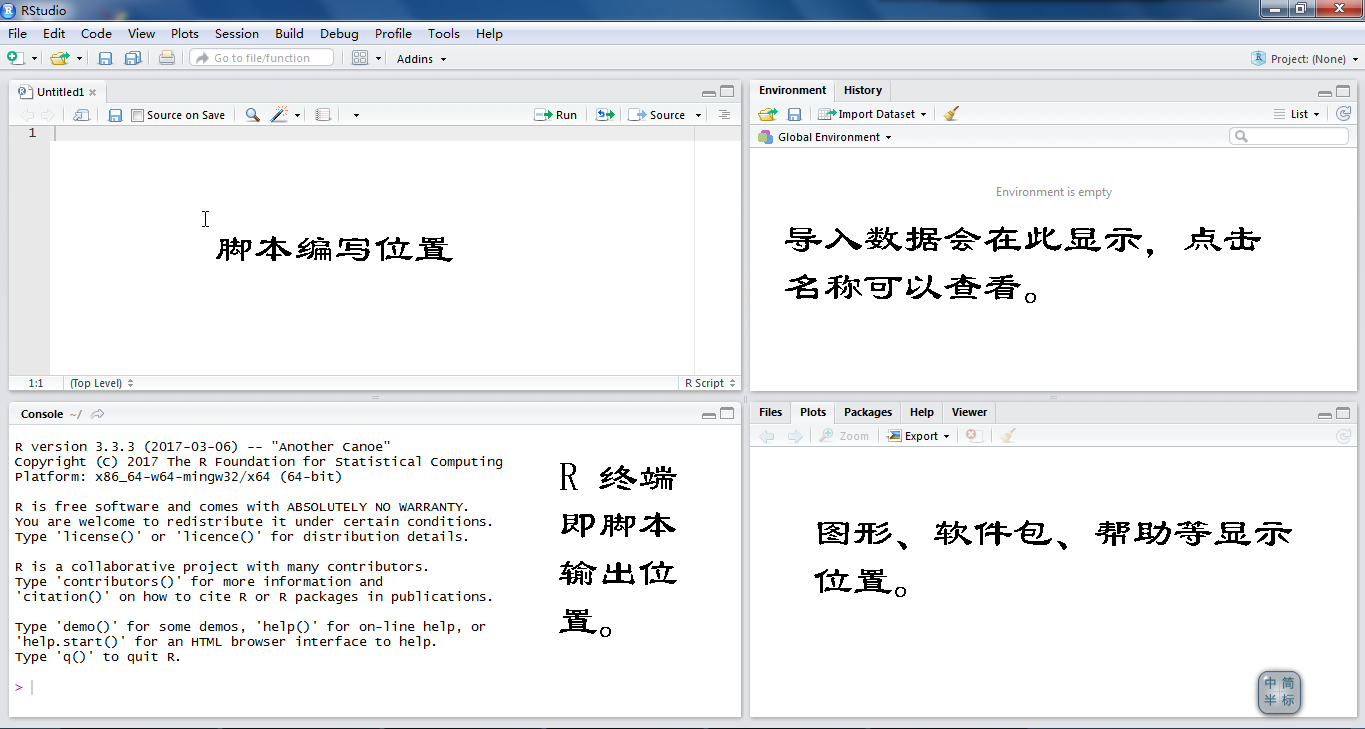
\includegraphics[width=4.55in]{images/rstudio} \caption{Rstudio 界面及功能}\label{fig:unnamed-chunk-2}
\end{figure}

本文的主要内容并非介绍这些软件的功能,因此,关于软件的操作部分请仔细阅读相关资料,网络上有大量的免费资源及教程,有需要的同学可自行搜索。

\begin{quote}
注:R 与 Rstudio 均非我公司产品,而且均免费或者有免费版本,因此请勿邮件或电话索要此两款软件。
\end{quote}

\cleardoublepage

\hypertarget{batch_question}{%
\chapter{批量处理光合测定数据}\label{batch_question}}

对于多数人来讲,一个季节用光合仪测量的数据文件至少是两位数的,处理起来非常不方便,针对这个问题,简单写了一个批量读取 LI-6400 和 LI-6800 原始数据的包(因为现有的容易实现的读取 excel 格式的包还不支持 6800 和 6400 这种形式的公式计算)\footnote{特别注意,原始数据可以用文本编辑器打开,但为了方便使用这个软件包,准确输入与行号相关的参数,建议您使用带行号显示的软件,例如 windows 下的 notepad++},使用非常简单,同时也适合处理未关闭数据文件而导致的无法生成 excel 格式的数据时的问题。

\hypertarget{install_readphoto}{%
\section{安装}\label{install_readphoto}}

暂时只有我的 github repo 中的版本:

\begin{Shaded}
\begin{Highlighting}[]
\NormalTok{devtools}\OperatorTok{::}\KeywordTok{install_github}\NormalTok{(}\StringTok{"zhujiedong/readphoto"}\NormalTok{)}
\end{Highlighting}
\end{Shaded}

\hypertarget{batch64}{%
\section{6400 数据整合}\label{batch64}}

基本参数如下:

\begin{Shaded}
\begin{Highlighting}[]
\KeywordTok{library}\NormalTok{(readphoto)}
\NormalTok{df64  <-}\StringTok{ }\KeywordTok{read_bat_6400}\NormalTok{(}\StringTok{"./data/6400"}\NormalTok{, }\DataTypeTok{header_line =} \DecValTok{17}\NormalTok{, }\DataTypeTok{data_start =} \DecValTok{27}\NormalTok{)}
\end{Highlighting}
\end{Shaded}

数据输出如下所示(仅显示前8列数据):

\begin{table}[t]

\caption{\label{tab:unnamed-chunk-5}LI-6400 批量整合数据}
\centering
\begin{tabular}{llllrrrrr}
\toprule
  & files & Obs & HHMMSS & FTime & EBal. & Photo & Cond & Ci\\
\midrule
1 & aci & 1 & 10:55:14 & 483.0 & 0 & 6.990 & 0.0831 & 251.0\\
4 & aci & 2 & 10:57:35 & 623.5 & 0 & 5.160 & 0.0853 & 192.0\\
7 & aci & 3 & 10:59:55 & 763.5 & 0 & 3.140 & 0.0881 & 136.0\\
10 & aci & 4 & 11:02:26 & 914.5 & 0 & 0.910 & 0.0927 & 81.9\\
13 & aci & 5 & 11:04:46 & 1055.0 & 0 & -0.167 & 0.0966 & 52.7\\
\addlinespace
16 & aci & 6 & 11:07:23 & 1211.5 & 0 & 5.240 & 0.1010 & 305.0\\
19 & aci & 7 & 11:09:43 & 1352.0 & 0 & 6.610 & 0.1040 & 284.0\\
22 & aci & 8 & 11:12:04 & 1492.5 & 0 & 9.280 & 0.1050 & 438.0\\
25 & aci & 9 & 11:14:24 & 1633.0 & 0 & 10.200 & 0.1020 & 616.0\\
28 & aci & 10 & 11:16:44 & 1772.5 & 0 & 10.500 & 0.0943 & 795.0\\
\addlinespace
31 & aci & 11 & 11:19:49 & 1958.0 & 0 & 10.700 & 0.0853 & 970.0\\
34 & aci & 12 & 11:22:09 & 2097.5 & 0 & 11.100 & 0.0812 & 1150.0\\
41 & aq & 2 & 10:12:52 & 737.5 & 0 & 6.450 & 0.0700 & 239.0\\
44 & aq & 3 & 10:15:12 & 878.0 & 0 & 6.450 & 0.0684 & 235.0\\
47 & aq & 4 & 10:17:32 & 1017.5 & 0 & 5.960 & 0.0655 & 241.0\\
\bottomrule
\end{tabular}
\end{table}

如果想另存为 csv 格式:

\begin{Shaded}
\begin{Highlighting}[]
\KeywordTok{write.csv}\NormalTok{(df64, }\StringTok{"./combined.csv"}\NormalTok{)}
\end{Highlighting}
\end{Shaded}

header\_line 表示你数据表头所在行,data\_start 表示你数据起始行,Obs = 1 时所在行,不含表头。这个也要确认好了,不同的测量不能放在一起(当然一般不会出现这种情况,同一台仪器,处理数据当然是希望 aci 和 aci 在一起,lrc 和 lrc 在一起,调查测量和调查测量在一起),不同的测量可能起始行不同,这样就会报错,特别需要注意的是,目前路径写法仅支持 ``/'' 分隔,不能使用 ``\textbackslash{}`` 作为分隔。例如在数据放在 D 盘的 6400 文件夹下,那么写法应为''d:/6400", 不能为 \textbf{``d:\textbackslash{}6400''}, 尽管后者对 R 是合法的,主要是因为我要区分你不同数据来源的文件是哪个,也即下文提到的 \texttt{df\$files} 列。

其中,数据的来源在表格中第一列,叫做 files,是数据来源的文件名(即你起的名字),例如本例中你看到的 aci 是我之前数据里面 aci 响应曲线的数据。

这些数据可以用于后文相关的分析中,尤其是像 \texttt{fitacis} 这样的函数,因为本质上他们都是符合 \texttt{tidyverse} 样式的数据。

\hypertarget{batch68}{%
\section{LI-6800 数据整合}\label{batch68}}

相比 6400, 6800 参数要少,导入需要两行命令即可:

\begin{Shaded}
\begin{Highlighting}[]
\KeywordTok{library}\NormalTok{(readphoto)}
\NormalTok{df <-}\StringTok{ }\KeywordTok{read_bat_6800}\NormalTok{(}\StringTok{"./data/6800"}\NormalTok{, }\DataTypeTok{data_start =} \DecValTok{56}\NormalTok{)}
\end{Highlighting}
\end{Shaded}

其中就两个参数,第一个为 LI-6800 \textbf{原始数据}所在的文件夹,即文件夹内\textbf{包含且仅包含 LI-6800 的原始数据},不要放其他文件,不要放 excel 数据。第二个参数即为你原始数据中测量数据的起始行,例如本例中使用数据测量值从 56 行开始。

数据输出如下所示(仅显示前8列数据):

\begin{table}[t]

\caption{\label{tab:unnamed-chunk-8}LI-6800 批量整合数据}
\centering
\begin{tabular}{lrrrlrrr}
\toprule
files & obs & time & elapsed & date & plot & plant & TIME\\
\midrule
aci & 1 & 1513614617 & 0.0 & 20171218 10:30:16 & 1 & 1 & 1513614617\\
aci & 2 & 1513614731 & 114.0 & 20171218 10:32:10 & 1 & 1 & 1513614731\\
aci & 3 & 1513614886 & 269.0 & 20171218 10:34:45 & 1 & 1 & 1513614886\\
aci & 4 & 1513615008 & 391.0 & 20171218 10:36:47 & 1 & 1 & 1513615008\\
aci & 5 & 1513615127 & 510.0 & 20171218 10:38:46 & 1 & 1 & 1513615127\\
\addlinespace
aci & 6 & 1513615287 & 670.5 & 20171218 10:41:27 & 1 & 1 & 1513615287\\
aci & 7 & 1513615410 & 793.0 & 20171218 10:43:29 & 1 & 1 & 1513615410\\
aci & 8 & 1513615566 & 949.0 & 20171218 10:46:05 & 1 & 1 & 1513615566\\
aci & 9 & 1513615701 & 1084.0 & 20171218 10:48:20 & 1 & 1 & 1513615701\\
aci & 10 & 1513615831 & 1214.0 & 20171218 10:50:30 & 1 & 1 & 1513615831\\
\addlinespace
aci & 11 & 1513615940 & 1323.0 & 20171218 10:52:19 & 1 & 1 & 1513615940\\
aci & 12 & 1513616064 & 1447.4 & 20171218 10:54:24 & 1 & 1 & 1513616064\\
lrc & 1 & 1513612721 & 0.0 & 20171218 09:58:40 & 1 & 1 & 1513612721\\
lrc & 2 & 1513612832 & 111.0 & 20171218 10:00:31 & 1 & 1 & 1513612832\\
lrc & 3 & 1513612941 & 220.0 & 20171218 10:02:20 & 1 & 1 & 1513612941\\
\bottomrule
\end{tabular}
\end{table}

其他注意事项见 LI-6400 数据整合部分

\hypertarget{recompute_raw}{%
\section{重计算功能}\label{recompute_raw}}

如果只是将原始数据批量处理,那么在遇到叶片不能充满叶室的情况时会很麻烦,这里我们提供了重新计算功能,重新计算的参数包括光合速率,蒸腾速率,对水的气孔导度以及胞间二氧化碳浓度,当然计算他们所需要的一些中间数值也做了重计算,只不过多数时候我们用不到,我们仅看这四项。

\hypertarget{recompute6400}{%
\subsection{LI-6400 数据重计算}\label{recompute6400}}

参数的重计算函数为 \texttt{recomp\_6400}, 其参数除了 \texttt{read\_bat\_6400} 所包含的参数外,还有叶面积 S, 以及叶片正反面的气孔比例,默认值分别为 6 和 0.5。

\begin{Shaded}
\begin{Highlighting}[]
\KeywordTok{library}\NormalTok{(readphoto)}
\NormalTok{x1 <-}\StringTok{ }\KeywordTok{read_bat_6400}\NormalTok{(}\StringTok{"./data/6400"}\NormalTok{)}
\NormalTok{y1 <-}\StringTok{ }\KeywordTok{recomp_6400}\NormalTok{(}\StringTok{"./data/6400"}\NormalTok{, }\DataTypeTok{header_line =} \DecValTok{17}\NormalTok{, }\DataTypeTok{data_start =} \DecValTok{27}\NormalTok{, }\DataTypeTok{S =} \DecValTok{6}\NormalTok{, }\DataTypeTok{K =} \FloatTok{0.5}\NormalTok{)}

\NormalTok{x1}\OperatorTok{$}\NormalTok{Photo }\OperatorTok{-}\StringTok{ }\NormalTok{y1}\OperatorTok{$}\NormalTok{Photo}
\end{Highlighting}
\end{Shaded}

\begin{verbatim}
##  [1] -0.0008873753  0.0026900500 -0.0012036469  0.0003483414  0.0006122641
##  [6] -0.0113872639 -0.0020986076  0.0004962787  0.0188727482 -0.0294595908
## [11] -0.0436611445 -0.0339083408  0.0046772165  0.0036653298  0.0030397988
## [16] -0.0105901673  0.0040624956  0.0017317049 -0.0073252290  0.0054977377
## [21]  0.0039736503  0.0021704065  0.0046772165  0.0036653298  0.0030397988
## [26] -0.0105901673  0.0040624956  0.0017317049 -0.0073252290  0.0054977377
## [31]  0.0039736503  0.0021704065
\end{verbatim}

\begin{Shaded}
\begin{Highlighting}[]
\NormalTok{x1}\OperatorTok{$}\NormalTok{Trmmol }\OperatorTok{-}\StringTok{ }\NormalTok{y1}\OperatorTok{$}\NormalTok{Trmmol}
\end{Highlighting}
\end{Shaded}

\begin{verbatim}
##  [1] -2.998596e-04  1.407338e-04  3.189451e-05 -4.586467e-04 -3.836822e-04
##  [6]  5.402725e-04 -2.344852e-04 -7.684772e-05  5.979599e-04 -6.534341e-04
## [11] -6.779145e-04  2.469749e-04  3.812201e-04  2.313957e-04  3.508312e-04
## [16] -2.794358e-04 -5.406530e-04  5.230606e-04 -9.183370e-04  7.638850e-04
## [21] -2.578893e-04  2.203045e-04  3.812201e-04  2.313957e-04  3.508312e-04
## [26] -2.794358e-04 -5.406530e-04  5.230606e-04 -9.183370e-04  7.638850e-04
## [31] -2.578893e-04  2.203045e-04
\end{verbatim}

\begin{Shaded}
\begin{Highlighting}[]
\NormalTok{x1}\OperatorTok{$}\NormalTok{Cond }\OperatorTok{-}\StringTok{ }\NormalTok{y1}\OperatorTok{$}\NormalTok{Cond}
\end{Highlighting}
\end{Shaded}

\begin{verbatim}
##  [1] -1.974217e-04 -3.594216e-04 -3.779119e-04 -3.806675e-04 -3.201411e-04
##  [6] -1.483324e-04 -7.803345e-04 -2.671018e-04  1.028977e-04 -3.966192e-04
## [11] -3.190769e-04 -2.314266e-04 -2.746300e-04  1.094050e-05 -4.584791e-05
## [16] -1.084094e-04 -1.827768e-04 -1.344969e-04 -1.714096e-04 -8.180257e-05
## [21] -4.687906e-05 -1.000424e-04 -2.746300e-04  1.094050e-05 -4.584791e-05
## [26] -1.084094e-04 -1.827768e-04 -1.344969e-04 -1.714096e-04 -8.180257e-05
## [31] -4.687906e-05 -1.000424e-04
\end{verbatim}

\begin{Shaded}
\begin{Highlighting}[]
\NormalTok{x1}\OperatorTok{$}\NormalTok{Ci}\OperatorTok{-}\NormalTok{y1}\OperatorTok{$}\NormalTok{Ci}
\end{Highlighting}
\end{Shaded}

\begin{verbatim}
##  [1]  0.434643936 -0.297820404 -0.308200950 -0.007847373 -0.035490198
##  [6]  0.433706824 -0.416734067 -0.052089770  0.147655545 -0.315797917
## [11] -0.271335987 -0.228968795  0.356519198  0.311487646  0.052196075
## [16]  0.557128947  0.058563406  0.300198435  0.052607786  0.339000061
## [21] -0.252622980 -0.494554616  0.356519198  0.311487646  0.052196075
## [26]  0.557128947  0.058563406  0.300198435  0.052607786  0.339000061
## [31] -0.252622980 -0.494554616
\end{verbatim}

\begin{Shaded}
\begin{Highlighting}[]
\CommentTok{# half of original the area}
\NormalTok{y1 <-}\StringTok{ }\KeywordTok{recomp_6400}\NormalTok{(}\StringTok{"./data/6400"}\NormalTok{,  }\DataTypeTok{header_line =} \DecValTok{17}\NormalTok{, }\DataTypeTok{data_start =} \DecValTok{27}\NormalTok{, }\DataTypeTok{S =} \DecValTok{3}\NormalTok{, }\DataTypeTok{K =} \FloatTok{0.5}\NormalTok{)}
\NormalTok{y1}\OperatorTok{$}\NormalTok{Photo}\OperatorTok{/}\NormalTok{x1}\OperatorTok{$}\NormalTok{Photo}
\end{Highlighting}
\end{Shaded}

\begin{verbatim}
##  [1] 2.000254 1.998957 2.000767 1.999234 2.007333 2.004346 2.000635
##  [8] 1.999893 1.996299 2.005611 2.008161 2.006110 1.998550 1.998863
## [15] 1.998980 2.003671 1.998391 1.999240 2.003866 1.995584 1.994199
## [22] 2.010360 1.998550 1.998863 1.998980 2.003671 1.998391 1.999240
## [29] 2.003866 1.995584 1.994199 2.010360
\end{verbatim}

\begin{Shaded}
\begin{Highlighting}[]
\CommentTok{# test with random area less than six}
\NormalTok{area <-}\StringTok{ }\DecValTok{6} \OperatorTok{-}\StringTok{ }\KeywordTok{runif}\NormalTok{(}\DecValTok{32}\NormalTok{, }\DecValTok{1}\NormalTok{, }\DecValTok{3}\NormalTok{)}
\NormalTok{y1 <-}\StringTok{ }\KeywordTok{recomp_6400}\NormalTok{(}\StringTok{"./data/6400"}\NormalTok{,  }\DataTypeTok{header_line =} \DecValTok{17}\NormalTok{, }\DataTypeTok{data_start =} \DecValTok{27}\NormalTok{, }\DataTypeTok{S =}\NormalTok{ area, }\DataTypeTok{K =} \FloatTok{0.5}\NormalTok{)}
\NormalTok{y1}\OperatorTok{$}\NormalTok{Photo}\OperatorTok{/}\NormalTok{x1}\OperatorTok{$}\NormalTok{Photo}
\end{Highlighting}
\end{Shaded}

\begin{verbatim}
##  [1] 1.526797 1.955327 1.846813 1.485734 1.254099 1.942496 1.397630
##  [8] 1.831466 1.328321 1.621659 1.424022 1.309466 1.386968 1.411053
## [15] 1.933386 1.574224 1.206083 1.339832 1.575369 1.251569 1.204440
## [22] 1.799651 1.249103 1.450440 1.520502 1.523471 1.824935 1.229340
## [29] 1.629910 1.711272 1.233337 1.800134
\end{verbatim}

我们看到各个值之差非常小,因为我们使用的是相同的叶面积,理论上这两次读数的差异应为 0, 但在实际计算过程中,有小数点位数的影响,所以某些值不完全为 0,但该差值足够小。我们将所有的数据叶面积减半后,二者比值也约等于 2.

\hypertarget{recompute6800}{%
\subsection{LI-6800 数据重计算}\label{recompute6800}}

参数的重计算函数为 \texttt{recomp\_6800}, 其参数除了 \texttt{read\_bat\_6800} 所包含的参数外,还有叶面积 S, 以及叶片正反面的气孔比例,默认值分别为 6 和 0.5。

\begin{Shaded}
\begin{Highlighting}[]
\KeywordTok{library}\NormalTok{(readphoto)}
\NormalTok{x3 <-}\StringTok{ }\KeywordTok{read_bat_6800}\NormalTok{(}\StringTok{"./data/6800"}\NormalTok{)}
\NormalTok{y3 <-}\StringTok{ }\KeywordTok{recomp_6800}\NormalTok{(}\StringTok{"./data/6800"}\NormalTok{, }\DataTypeTok{data_start =} \DecValTok{56}\NormalTok{, }\DataTypeTok{S =} \DecValTok{6}\NormalTok{, }\DataTypeTok{K =} \FloatTok{0.5}\NormalTok{)}

\NormalTok{x3}\OperatorTok{$}\NormalTok{A }\OperatorTok{-}\StringTok{ }\NormalTok{y3}\OperatorTok{$}\NormalTok{A}
\end{Highlighting}
\end{Shaded}

\begin{verbatim}
##  [1] 0 0 0 0 0 0 0 0 0 0 0 0 0 0 0 0 0 0 0 0 0 0 0 0 0 0 0 0
\end{verbatim}

\begin{Shaded}
\begin{Highlighting}[]
\NormalTok{x3}\OperatorTok{$}\NormalTok{E }\OperatorTok{-}\StringTok{ }\NormalTok{y3}\OperatorTok{$}\NormalTok{E}
\end{Highlighting}
\end{Shaded}

\begin{verbatim}
##  [1] 0 0 0 0 0 0 0 0 0 0 0 0 0 0 0 0 0 0 0 0 0 0 0 0 0 0 0 0
\end{verbatim}

\begin{Shaded}
\begin{Highlighting}[]
\NormalTok{x3}\OperatorTok{$}\NormalTok{gsw }\OperatorTok{-}\StringTok{ }\NormalTok{y3}\OperatorTok{$}\NormalTok{gsw}
\end{Highlighting}
\end{Shaded}

\begin{verbatim}
##  [1] -0.01231889 -0.01271539 -0.01330812 -0.01416506 -0.01491902
##  [6] -0.01586479 -0.01566857 -0.01545520 -0.01563183 -0.01537453
## [11] -0.01494554 -0.01433677 -0.02284560 -0.02291318 -0.02268118
## [16] -0.02266862 -0.02250392 -0.02213352 -0.02061493 -0.02006006
## [21] -0.01856400 -0.01678649 -0.01591079 -0.01457109 -0.01322393
## [26] -0.02345109 -0.02312573 -0.02227497
\end{verbatim}

\begin{Shaded}
\begin{Highlighting}[]
\NormalTok{x3}\OperatorTok{$}\NormalTok{Ci}\OperatorTok{-}\NormalTok{y3}\OperatorTok{$}\NormalTok{Ci}
\end{Highlighting}
\end{Shaded}

\begin{verbatim}
##  [1]  4.43187567  3.13678828  1.78620310  0.49515242 -0.08437000
##  [6]  3.51420195  3.66611259  5.56360761  6.76351008  7.70784028
## [11]  8.45263315  9.25926640  2.58978666  2.52629775  2.49784796
## [16]  2.38619050  2.23225682  1.92200639  1.29213044  0.92018214
## [21]  0.76352452  0.55412066  0.20248257 -0.08219604 -0.26216626
## [26]  2.36039345  2.40636618  2.54353742
\end{verbatim}

\begin{Shaded}
\begin{Highlighting}[]
\CommentTok{# half of original the area}
\NormalTok{y3 <-}\StringTok{ }\KeywordTok{recomp_6800}\NormalTok{(}\StringTok{"./data/6800"}\NormalTok{, }\DataTypeTok{data_start =} \DecValTok{56}\NormalTok{, }\DataTypeTok{S =} \DecValTok{3}\NormalTok{, }\DataTypeTok{K =} \FloatTok{0.5}\NormalTok{)}
\NormalTok{y3}\OperatorTok{$}\NormalTok{A}\OperatorTok{/}\NormalTok{x3}\OperatorTok{$}\NormalTok{A}
\end{Highlighting}
\end{Shaded}

\begin{verbatim}
##  [1] 2 2 2 2 2 2 2 2 2 2 2 2 2 2 2 2 2 2 2 2 2 2 2 2 2 2 2 2
\end{verbatim}

\begin{Shaded}
\begin{Highlighting}[]
\CommentTok{# test with random area less than six}
\NormalTok{area <-}\StringTok{ }\DecValTok{6} \OperatorTok{-}\StringTok{ }\KeywordTok{runif}\NormalTok{(}\DecValTok{28}\NormalTok{, }\DecValTok{1}\NormalTok{, }\DecValTok{3}\NormalTok{)}
\NormalTok{y3 <-}\StringTok{ }\KeywordTok{recomp_6800}\NormalTok{(}\StringTok{"./data/6800"}\NormalTok{, }\DataTypeTok{data_start =} \DecValTok{56}\NormalTok{, }\DataTypeTok{S =}\NormalTok{ area, }\DataTypeTok{K =} \FloatTok{0.5}\NormalTok{)}
\NormalTok{y3}\OperatorTok{$}\NormalTok{A}\OperatorTok{/}\NormalTok{x3}\OperatorTok{$}\NormalTok{A}
\end{Highlighting}
\end{Shaded}

\begin{verbatim}
##  [1] 1.294310 1.798840 1.696216 1.320046 1.916465 1.375307 1.510122
##  [8] 1.901511 1.337287 1.404141 1.856641 1.251275 1.739408 1.830320
## [15] 1.359718 1.282576 1.507111 1.260038 1.488009 1.546680 1.587274
## [22] 1.484716 1.686316 1.255972 1.821984 1.543852 1.540470 1.822845
\end{verbatim}

测量结果相比 6400 的数据,某些值差异略大,我仔细核对过公式,并无问题,可能仅仅是小数点后数据的原因,如果童鞋们发现我这里有错误,可以提交 github 或者邮箱发送给我,便于我改正。

\cleardoublepage

\hypertarget{response_fit}{%
\chapter{\texorpdfstring{CO\textsubscript{2} 响应曲线的拟合}{CO2 响应曲线的拟合}}\label{response_fit}}

\hypertarget{fvcb_mod}{%
\section{FvCB 模型}\label{fvcb_mod}}

在 \texttt{plantecophys} 包中使用的模型为 \citet{Farquhar1980A} 建立的 C3 植物模型 FvCB,其基于 C3 植物碳反应的三个阶段:

\begin{itemize}
\item
  核酮糖-1,5-双磷酸羧化酶/加氧酶 (Rubisco)的催化下, 核酮糖-1,5-双磷酸(RuBP)与 CO\textsubscript{2}发生羧化作用, 生成3-磷酸甘油酸(PGA)。
\item
  在腺苷三磷酸(ATP)和还原型烟酰胺腺嘌呤 二核苷酸磷酸(NADPH)的作用下, PGA被还原成磷 酸丙糖(TP)。每6个TP中有1个输出到细胞液中,
  用 于蔗糖或者淀粉的合成。
\item
  剩下的5个TP 在ATP的作用下再生为 3 个RuBP。一部分再生的 RuBP在Rubisco的催化下被氧化成PGA和2-磷酸乙 醇酸,
  2-磷酸乙醇酸在ATP的作用下形成PGA, 并且 释放CO\textsubscript{2} (光呼吸)。
\end{itemize}

在光照下, C3 植物净光合速率 (A) 取决于 3 个同时存在的速率: RuBP羧化速率(Vc)、RuBP氧化速率 (或光呼吸速率,
Vo)和线粒体在光照下的呼吸速率 (或明呼吸速率, Rd; 此名为了与暗呼吸速率对应和区分)。RuBP氧化过程中每结合1 mol
O\textsubscript{2} 就会释放 0.5 mol CO\textsubscript{2} 。因此, 净光合速率 A 的计算为:

\begin{figure}
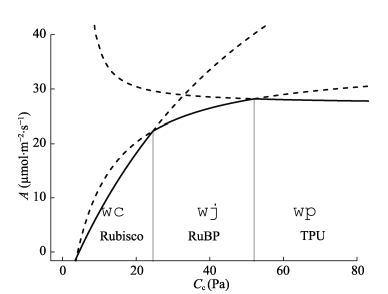
\includegraphics[width=1\linewidth]{images/fvcb} \caption{光合速率的不同的限制阶段}\label{fig:fvcb}
\end{figure}

\begin{equation}
A\ =V_{c}\ -0.5V_{o}\ -\ R_{d}
\label{eq:aeta}
\end{equation}

线粒体Rd不同于暗呼吸速率(Rn )。Rn是叶片在 黑暗中的线粒体呼吸速率, 随着光照的增加, 线粒体呼吸速率下降。因此 Rd \textless{}
Rn 在黑暗条件下测定的叶 片 CO\textsubscript{2} 交换速率即 Rn , 但是 Rd 的测定比较困难, 因为光照条件下 Rd 与
Vc、Vo 同时存在。\citet{Hikosaka2006Temperature} 总结了几种测定
Rd 的方法,式 \eqref{eq:aeta} 又可表达为:

\begin{equation}
A\ =V_{c}\ (1\ -0.5\alpha)\ R_{d}
\label{eq:achange}
\end{equation}

式 \eqref{eq:achange} 中 \(\alpha\) 为氧化速率和羧化速率的比值,由 Rubisco 动力学常数确定:

\begin{equation}
\begin{split}
\alpha & =\frac{V_{O}}{V_{C}}\\
& = \frac{O}{C_c} \times \frac{V_{omax} K_c}{V_{cmax}K_{o}}\\
& = \frac{O}{C_{c}} \times \frac{1}{S_{\frac{c}{o}}}
\end{split}
\label{eq:dynamic}
\end{equation}

式 \eqref{eq:dynamic} 中,Cc 和 O 分别为叶绿体部位 CO\textsubscript{2} 和 O\textsubscript{2} 浓度。Cc 和
O 通常以气体摩尔分数 (\(\mu mol\text{·}mol^{-1}\) ) 或分压 (Pa) 表示, 但光合过程是在叶绿体的液相基质中发生的,
用分压表示更加恰当。Kc 与 Ko 为 Rubisco 羧化(氧化)的米氏常数, 代表了羧化(氧化)速率达到最大羧化(氧化)速率一半时的
CO\textsubscript{2} 和 \(O_{2}\) 浓度。是 Rubisco 特异性因子, \(S_{\frac{c}{o}}\)表示 Rubisco
对CO\textsubscript{2} 和 \(O_{2}\) 的偏好程度。

当 A = Rd , 即 RuBP 羧化的 CO\textsubscript{2} 吸收速率刚好 等于 RuBP 氧化的 CO\textsubscript{2} 释放速率
(Vc = 0.5Vo ) 时, \(\alpha\) = 0.5。此时叶绿体的 CO\textsubscript{2} 浓度就是叶绿体 CO\textsubscript{2}
光合补偿点, 标记为 \(\Gamma^{*}\)。即:

\begin{equation}
\Gamma^{*}\ =\ \frac{0.5O}{S_{\frac{c}{o}}}
\label{eq:com}
\end{equation}

由公式 \eqref{eq:dynamic}和公式 \eqref{eq:com}可得:

\begin{equation}
\alpha =\frac{2\Gamma^{*}}{C_{c}}
\label{eq:combine}
\end{equation}

代入公式 \eqref{eq:achange} 得到:

\begin{equation}
A\ =V_{c}\ (1\ -\frac{\Gamma^{*}}{C_{c}})\ R_{d}
\label{eq:combine2}
\end{equation}

在 Cc 浓度很低的时候,RuBP 供应充足 (图 \ref{fig:fvcb} Rubisco 阶段),Vc 等于 Rubisco
所能支持的羧化速率 w\textsubscript{c},:

\begin{equation}
w_{c}\ =\ \frac{V_{cmax\ }C_{c}}{C_{c\ }+\ K_{c\ }(1\ +\ \frac{O}{K_{o}})}
\label{eq:wc}
\end{equation}

随着 Cc 浓度的增加,Rubisco 支持的羧化速率超过了 RuBP 供应速率, Vc 受 RuBP 再生速率的限制(图 \ref{fig:fvcb}
RuBP 阶段),此时 Vc 由 RuBP 的再生速率限制,而 RuBP 又由电子传递速率(J)决定,故:

\begin{equation}
w_{j}\ =\ \frac{J\ C_{c}}{4C_{c\ }+\ 8\Gamma^{*}}
\label{eq:wj}
\end{equation}

当 Cc 浓度很高,光合磷酸化超过了淀粉和蔗糖的合成速率的时候,Vc 受到 TP 利用速率(Vp)的限制(图 \ref{fig:fvcb}
TPU 阶段),一般情况下,

\begin{equation}
w_{p\ }=\ \frac{3V_{p}C_{c}}{C_{c}-\Gamma^{*}}
\label{eq:wp}
\end{equation}

最终,C3 植物叶片的光合速率 A 由 w\textsubscript{c}、w\textsubscript{j}、w\textsubscript{p}
的最小者决定(图 \ref{fig:fvcb} 实现部分),当c \textgreater{} \(\Gamma^{*}\)时:

\begin{equation}
A=min\{w_{c},w_{j,}w_{p}\}(1-\frac{\Gamma^{*}}{C_{c}})-R_{d}
\label{eq:fvcbfin}
\end{equation}

\hypertarget{co2_note}{%
\section{\texorpdfstring{CO\textsubscript{2} 响应曲线测量的注意事项}{CO2 响应曲线测量的注意事项}}\label{co2_note}}

尽管上文对其分段性做了数学上的解释,相比来讲,不是那么通俗易懂,根据 \citet{matthew2018} 文章中的内容,我们后面两小节的内容对其进行概述:

\hypertarget{model_3}{%
\subsection{分段性}\label{model_3}}

与光响应曲线不同, A/Ci 曲线是分段的,这也增加了其复杂性,在其最初阶段,\(CO_2\) 浓度较低,在此阶段, Rubisco 更多的与 \(O_2\) 结合,因此,即使是较小浓度的 \(CO_2\) 的增加,也会显著提高羧化速率,我们将此阶段称之为 \(CO_2\) (\citet{Wullschleger1993Biochemical}) 限制或 Rubisco 限制 (\citet{Long2003Gas})。净光合速率 A 与 Ci 在此阶段斜率比较陡峭,实践中往往利用计算该斜率来计算 \(V_{cmax}\)。

在较高的 \(CO_2\) 浓度下,曲线斜率开始便的平缓,作为底物的 \(CO_2\) 已经不在是限制因素,随着羧化速率达到最大,RUBP 的量成为了其限制因素,而 RUBP 的再生速率受最大电子传递速率 \(J_{max}\) 的限制。此时曲线的弯曲点由 \(V_{cmax}\) 限制转变为 \(J_{max}\),许多研究中将饱和光下和 \(CO_2\) 浓度下测量的光合速率称之为做大光合速率(\citet{heath2005rising})。而另一些研究中将最大光合速率定义为外界 \(CO_2\) 时,在饱和光强下达到的最大光合速率(\citet{marshall1980a})。这些术语上的差别需要注意。

在之后,有可能继续观测到磷酸盐限制 RUBP 再生的情况,导致光合速率的下降。因为此时大量的磷酸丙糖与正磷酸盐结合,导致 ATP 合成受限制(\citet{ellsworth2015phosphorus})。这就是 TPU 限制阶段。

\hypertarget{note_detail}{%
\subsection{测量注意事项}\label{note_detail}}

尽管您的操作是严格按照说明书操作的,但说明书是指仪器的正确操作方式,无法对所有测量都采用相同设置,要获得好的测量结果,有更多的因素需要注意:

使用 LI-6400 或 LI-6800 测量 A/Ci 曲线的过程也就是控制叶室或参比室气体浓度变化的过程,\textbf{只要诱导的时间足够},气孔会在相应设置的环境条件下开到足够大,这样 Ci 会随 Ca 而变化,一般来讲二者的比例为 0.7,但也可能在 0.5\textasciitilde{}0.7 间变化。

一般来讲,测量参数是在温度为 25 \(^{\circ}\)C 时获得,但实际测量过程中,因为外界温度过高或过低等无法控制叶室温度到 25 \(^{\circ}\)C,这其实并非严重的问题,因为这可以通过数学上的方法将计算参数标准化为 25 \(^{\circ}\)C 时的结果。所以,在测量时只需控制叶室温度稳定即可(通常为 20 \(^{\circ}\)C \textasciitilde{} 30 \(^{\circ}\)C 之间)。 此外就是控制恒定的 VPD 及一个饱和光强。另外就是需要注意,开始测量之前,必须在外界环境的 \(CO_2\) 浓度下诱导足够长的时间,使光合速率达到稳定,一般需要20 \textasciitilde{} 30 min。对于没有稳定的光保护机制的植物,一般不建议在 50 ppm 或更低的浓度下进行设置,此时饱和光强和建议的温度下,植物没有足够的底物进行光合作用,这样会因为光化学反应的降低发生氧化性损伤。\citet{centritto2003} 研究表明,长时间的在 50 ppm 下诱导气孔打开到最大时,可以观测到最大的气孔导度(非标准方式测量)。

对于存在干旱胁迫的测量,由于干旱会导致气孔关闭(\citet{lauteri2014}), 此时没有足够多的 \(CO_2\) 进入气孔,此时的测量是没有意义的,可在 50 ppm 诱导 1 h 等待气孔完全打开再快速升高 Ca 的值来进行测量(\citet{centritto2003})。该方法对于 \(V_{cmax}\) 不受影响而 \(J_{max}\) 降低的情况适用(\citet{Aganchich2009})。但在某些情况下,气孔关闭速度太快,无法完成整个 A/Ci 曲线过程 (Haworth2017)(需要考虑 LI-6800 RACiR)。更重要的是,如果想采用拟合方式求 gm,那么气孔必须完全打开使叶片对 \(CO_2\) 吸收的限制降到最低。对于灌溉情况良好的植物或者土壤水分情况比较好的植物,气孔不对高于外界浓度的 Ca 的升高而响应(\citet{haworth2015coordination}),这可能需要更多的测量点或延长测量点的时间间隔来提高曲线的分辨率。另外,测量点的数量也要根据研究而改变,例如重点测量 Vcamx 时,50 \textasciitilde{} 300 ppm 的数据点要多一些,而如果研究对象是土壤磷酸盐对植物生理的限制,那么 1600 \textasciitilde{} 2000 ppm 的数据点要适当增多。

一个更精确的了解植物生理指标的方法是将 A/Ci 曲线改为 A/Cc 曲线,但这需要了解 gm 数据。因为 Cc 通过如下方式计算:

\begin{equation}
C_c = C_i - \frac{A}{gm}
\label{eq:notecc}
\end{equation}

对于 gm 的计算,比较易操作的有几种:采用光合荧光联合测量的方式计算求得。当然也可以采用曲线拟合的方式,或者 \citet{yin2009using} 使用的方式,在低氧气体下,采用不同的光照水平求得。

此外,测量气体交换非常重要的误差来源就是气体的扩散,因为测量时,多数时间内外界气体浓度要高于叶室内的气体浓度,那么即使使用密封性非常好的材料,由外界高 \(CO_2\) 浓度气体向叶室低 \(CO_2\) 浓度气体的扩散无法避免,尤其是在连续长时间测量时该效应尤为明显,因此需要经常更换叶室垫圈。具体可以通过一些方法来校正(\citet{Flexas2007leak},rodeghiero2007major),但如果采用 LI-6800 测量这将不是问题,它采用的叶室增加技术并根据测量的漏气情况对结果自动修正。

\hypertarget{plantecophys}{%
\section{\texorpdfstring{\texttt{plantecophys} 软件包}{plantecophys 软件包}}\label{plantecophys}}

Remko A. Duursma 在2015年发表了一篇文章 \citet{Duursma2015Plantecophys},\texttt{plantecophys} 是其开发的一个R包工具集,用于对叶片气体交换数据进行分析和建模。实现了如下功能:

\begin{itemize}
\tightlist
\item
  CO\textsubscript{2} 响应曲线 (A-Ci curves) 的拟合、作图及模拟。
\item
  不同气孔导度模型。
\item
  根据 Cowan-Farquhar 的假设估算最适的气孔导度。
\item
  耦合气体交换模型的实现。
\item
  基于 Ci 模拟 C4 光合。
\item
  RHtoVPD:常用单位的转换(相对湿度、水汽压亏缺、露点温度)。
\end{itemize}

各参数的基本用法请参考后文内容,或官方帮助文档:

\href{https://cran.r-project.org/web/packages/plantecophys/plantecophys.pdf}{plantecophys}。

\hypertarget{fit6400}{%
\section{\texorpdfstring{LI-6400XT CO\textsubscript{2} 响应曲线的拟合}{LI-6400XT CO2 响应曲线的拟合}}\label{fit6400}}

LI-6400XT CO\textsubscript{2} 响应曲线的拟合需要借助 \texttt{plantecophys} 的 \texttt{fitaci} 实现,fitaci 函数为根据 FvCB 模型对 A-Ci 曲线的测量数据进行拟合,并估算 J\(_{max}\)、V\(_{cmax}\)、R\(_{d}\)及他们的标准差,并根据
\citet{Medlyn2002Temperature} 的方法考虑了温度的影响。

\hypertarget{fitaci_intro}{%
\subsection{fitaci 函数介绍}\label{fitaci_intro}}

\texttt{fitaci} 的用法如下\footnote{仅针对 C3 植物}:

\begin{Shaded}
\begin{Highlighting}[]
\KeywordTok{fitaci}\NormalTok{(data, }\DataTypeTok{varnames =} \KeywordTok{list}\NormalTok{(}\DataTypeTok{ALEAF =} \StringTok{"Photo"}\NormalTok{, }
  \DataTypeTok{Tleaf =} \StringTok{"Tleaf"}\NormalTok{, }\DataTypeTok{Ci =} \StringTok{"Ci"}\NormalTok{, }\DataTypeTok{PPFD =} \StringTok{"PARi"}\NormalTok{, }
  \DataTypeTok{Rd =} \StringTok{"Rd"}\NormalTok{), }\DataTypeTok{Tcorrect =} \OtherTok{TRUE}\NormalTok{, }\DataTypeTok{Patm =} \DecValTok{100}\NormalTok{, }
  \DataTypeTok{citransition =} \OtherTok{NULL}\NormalTok{, }\DataTypeTok{quiet =} \OtherTok{FALSE}\NormalTok{, }
  \DataTypeTok{startValgrid =} \OtherTok{TRUE}\NormalTok{, }\DataTypeTok{fitmethod =} 
  \KeywordTok{c}\NormalTok{(}\StringTok{"default"}\NormalTok{, }\StringTok{"bilinear"}\NormalTok{, }\StringTok{"onepoint"}\NormalTok{), }
  \DataTypeTok{algorithm =} \StringTok{"default"}\NormalTok{, }\DataTypeTok{fitTPU =} \OtherTok{FALSE}\NormalTok{, }
  \DataTypeTok{useRd =} \OtherTok{FALSE}\NormalTok{, }\DataTypeTok{PPFD =} \OtherTok{NULL}\NormalTok{, }\DataTypeTok{Tleaf =} \OtherTok{NULL}\NormalTok{, }
  \DataTypeTok{alpha =} \FloatTok{0.24}\NormalTok{, }\DataTypeTok{theta =} \FloatTok{0.85}\NormalTok{, }\DataTypeTok{gmeso =} \OtherTok{NULL}\NormalTok{, }
  \DataTypeTok{EaV =} \FloatTok{82620.87}\NormalTok{, }\DataTypeTok{EdVC =} \DecValTok{0}\NormalTok{, }\DataTypeTok{delsC =} \FloatTok{645.1013}\NormalTok{,}
  \DataTypeTok{EaJ =} \FloatTok{39676.89}\NormalTok{, }\DataTypeTok{EdVJ =} \FloatTok{2e+05}\NormalTok{, }
  \DataTypeTok{delsJ =} \FloatTok{641.3615}\NormalTok{, }\DataTypeTok{GammaStar =} \OtherTok{NULL}\NormalTok{, }
  \DataTypeTok{Km =} \OtherTok{NULL}\NormalTok{, }\DataTypeTok{id =} \OtherTok{NULL}\NormalTok{, ...)}

\CommentTok{## S3 method for class 'acifit'}
\KeywordTok{plot}\NormalTok{(x, }\DataTypeTok{what =} \KeywordTok{c}\NormalTok{(}\StringTok{"data"}\NormalTok{, }\StringTok{"model"}\NormalTok{, }\StringTok{"none"}\NormalTok{),}
     \DataTypeTok{xlim =} \OtherTok{NULL}\NormalTok{, }\DataTypeTok{ylim =} \OtherTok{NULL}\NormalTok{, }\DataTypeTok{whichA =} \KeywordTok{c}\NormalTok{(}
       \StringTok{"Ac"}\NormalTok{, }\StringTok{"Aj"}\NormalTok{, }\StringTok{"Amin"}\NormalTok{, }\StringTok{"Ap"}\NormalTok{), }\DataTypeTok{add =} \OtherTok{FALSE}\NormalTok{,}
\DataTypeTok{pch =} \DecValTok{19}\NormalTok{, }\DataTypeTok{addzeroline =} \OtherTok{TRUE}\NormalTok{, }\DataTypeTok{addlegend =} 
  \OperatorTok{!}\NormalTok{add, }\DataTypeTok{legendbty =} \StringTok{"o"}\NormalTok{,}\DataTypeTok{transitionpoint =} \OtherTok{TRUE}\NormalTok{, }
\DataTypeTok{linecols =} \KeywordTok{c}\NormalTok{(}\StringTok{"black"}\NormalTok{, }\StringTok{"blue"}\NormalTok{, }\StringTok{"red"}\NormalTok{), }\DataTypeTok{lwd =} \KeywordTok{c}\NormalTok{(}\DecValTok{1}\NormalTok{,}
\DecValTok{2}\NormalTok{), ...)}
\end{Highlighting}
\end{Shaded}

\emph{主要参数注释:}

\begin{itemize}
\tightlist
\item
  data:需要分析的数据,必须为 data.frame\footnote{具体参考 R 语言相关文档,为 R 语言最常用的数据格式}。
  格式。
\item
  varnames:数据的表头,此处函数默认的表头为 LI-6400 的表头,分析 LI-6400 的数据时可以不用填写,直接使用默认的参数即可\footnote{在 R 中,使用参数的值为默认值时可以不用填写该参数,例如使用默认选项分析 LI-6400 数据时,可只填写 data 项,具体参考
    R 的相关入门手册}。
\item
  Tcorrect:如果为 TRUE,那么 J\(_{max}\)、V\(_{cmax}\) 的结果为温度校正结果,若 Tcorrect = FALSE,则为测量温度下的结果。
\item
  Patm:为外界大气压。
\item
  citransition:参见详,若提供该选项,则 J\(_{max}\)、V\(_{cmax}\)
  的区域则分别拟合\footnote{为Rubisco和RuBP限制的Ci转换点,物种间差异较大,可以通过预实验确定}。
\item
  fitmethod:参见详解。
\item
  fitTPU:是否拟合 TPU 限制,默认为 FALSE,参见详解。
\item
  x:对于plot.acifit,x 为fitaci返回的对象,简单理解为 将 fitaci 函数拟合结果赋值给一个变量,此处plot函数实际上为plot.acifit。
\item
  what:利用基础做图工具,默认为对数据和模型进行作图。
\item
  whichA:默认为对所有的光合速率进行作图(Aj=Jmax-limited (蓝色), Ac=Vcmax- limited (红色),
  Hyperbolic minimum (黑色)), TPU-limited rate (Ap, 如果模型有计算结果)。
\end{itemize}

其他参数请参考 FvCB 模型 \citet{Farquhar1980A} 或查看 plantecophys 的帮助文档。

\hypertarget{fitaci_detail}{%
\subsubsection{fitaci函数详解}\label{fitaci_detail}}

\begin{itemize}
\item
  默认为非线性拟合,详见 \citet{Duursma2015Plantecophys}。
\item
  bilinear 方法使用两次线性拟合方法首先拟合 V\(_{cmax}\) 和 R\(_{d}\),然后在拟合J\(_{max}\),过渡点的选择为对所有数据拟合最适的点,类似 \citet{Gu2010Reliable} 的方法。该方法的优势时无论如何,都会返回拟合结果,尤其是非线性拟合失败时使用该方法,但若默认方法失败时,需首先检查是否数据存在问题。两种拟合方法的结果有轻微的差别\footnote{若默认拟合方法失败,数据也无问题,那么是非线性拟合初始值设定的原因}。
\item
  onepoint 参考 \citet{De2016A}。
\item
  citransition 使用时,数据将被区分为 V\(_{cmax}\) 限制(Ci \textless{}
  citransition )区域,以及 J\(_{max}\) 限制 (Ci \textgreater{} citransition) 区域。
\item
  fitTPU:如果要计算TPU,要设置 fitTPU = TRUE,并且 fittingmethod
  = ``bilinear''。但需要注意,当 TPU 被计算时,没有 J\(_{max}\) 限制的点的存在是可能的。TPU限制的发生是在A值不随
  CO\(_{2}\) 的增加而增加时发生的,因此计算 TPU 是否有返回值,取决于测量数据是否有此情况出现。
\end{itemize}

\hypertarget{plantecophy_use}{%
\section{\texorpdfstring{使用 \texttt{plantecophys} 拟合 LI-6400XT CO\textsubscript{2} 响应曲线数据}{使用 plantecophys 拟合 LI-6400XT CO2 响应曲线数据}}\label{plantecophy_use}}

\hypertarget{data6400}{%
\subsection{数据的前处理}\label{data6400}}

虽然 R 软件支持直接导入 xlsx 的数据,但因为 LI-6400XT 的数据记录文件内有其他空行或 remark 等内容,增加了处理代码的量,\textbf{故而推荐将其数据先整理为如表 \ref{tab:head6400} 样式,并另存为 csv 格式}\footnote{即仅保留测量值,删除其他所有头文件、空行、 remark 等信息}:

\begin{longtable}{rlrrrrrr}
\caption{\label{tab:head6400}推荐 LI-6400 整理后数据样式}\\
\toprule
Obs & HHMMSS & FTime & EBal. & Photo & Cond & Ci & Trmmol\\
\midrule
1 & 15:46:59 & 271.5 & 0 & 14.2848912 & 0.2730691 & 286.39751 & 2.226126\\
2 & 15:48:26 & 358.0 & 0 & 10.6562220 & 0.2826303 & 217.32002 & 2.292845\\
3 & 15:49:54 & 446.0 & 0 & 6.4525814 & 0.2909460 & 150.67623 & 2.361704\\
4 & 15:51:26 & 538.5 & 0 & 1.7971569 & 0.3057164 & 85.82530 & 2.459459\\
5 & 15:52:54 & 626.5 & 0 & -0.6575974 & 0.3150002 & 53.47985 & 2.515992\\
\addlinespace
6 & 15:54:50 & 742.5 & 0 & 15.4296572 & 0.3255415 & 292.56161 & 2.579840\\
\bottomrule
\end{longtable}

\hypertarget{fitaci-p}{%
\subsection{使用示例}\label{fitaci-p}}

\texttt{plantecophys} 并非 base 的安装包,首次使用需要从 \texttt{CRAN} 安装,可以使用图形界面安装,也可以直接用命令行安装\footnote{首次使用安装,更换电脑或者升级 R 软件后,如果没有拷贝 library,也需要运行安装命令},推荐同时安装依赖。

\begin{Shaded}
\begin{Highlighting}[]
\KeywordTok{install.packages}\NormalTok{(}\StringTok{"plantecophys"}\NormalTok{, }\DataTypeTok{dependencies =} \OtherTok{TRUE}\NormalTok{)}
\end{Highlighting}
\end{Shaded}

\begin{Shaded}
\begin{Highlighting}[]
\CommentTok{# 载入 plantecophys }
\KeywordTok{library}\NormalTok{(}\StringTok{"plantecophys"}\NormalTok{)}

\CommentTok{# 利用read.csv读取数据文件,}
\CommentTok{# 我的路径为当前工作路径的data文件夹内}
\NormalTok{aci <-}\StringTok{ }\KeywordTok{read.csv}\NormalTok{(}\StringTok{"./data/aci.csv"}\NormalTok{)}

\CommentTok{# 防止可能出现的NA值}
\NormalTok{aci <-}\StringTok{ }\KeywordTok{subset}\NormalTok{(aci, Obs }\OperatorTok{>}\StringTok{ }\DecValTok{0}\NormalTok{)}

\CommentTok{# 不修改默认参数对数据进行拟合}
\NormalTok{acifit <-}\StringTok{ }\KeywordTok{fitaci}\NormalTok{(aci)}
\CommentTok{# 查看拟合结果的参数名称,方便导出数据使用}
\KeywordTok{attributes}\NormalTok{(acifit)}
\end{Highlighting}
\end{Shaded}

\begin{verbatim}
## $names
##  [1] "df"             "pars"           "nlsfit"         "Tcorrect"      
##  [5] "Photosyn"       "Ci"             "Ci_transition"  "Ci_transition2"
##  [9] "Rd_measured"    "GammaStar"      "Km"             "kminput"       
## [13] "gstarinput"     "fitmethod"      "citransition"   "gmeso"         
## [17] "fitTPU"         "alphag"         "RMSE"           "runorder"      
## 
## $class
## [1] "acifit"
\end{verbatim}

\begin{Shaded}
\begin{Highlighting}[]
\CommentTok{# 查看拟合结果}
\KeywordTok{summary}\NormalTok{(acifit)}
\end{Highlighting}
\end{Shaded}

\begin{verbatim}
## Result of fitaci.
## 
## Data and predictions:
##            Ci      Ameas     Amodel         Ac        Aj   Ap       Rd VPD
## 5    53.47985 -0.6575974 -0.5146882 -0.3552036  0.000000 1000 0.159449 1.5
## 4    85.82530  1.7971569  1.9292621  2.0888575  5.068534 1000 0.159449 1.5
## 3   150.67623  6.4525814  6.4176037  6.5777528 12.755502 1000 0.159449 1.5
## 2   217.32002 10.6562220 10.5354626 10.6965875 17.519644 1000 0.159449 1.5
## 1   286.39751 14.2848912 14.3365887 14.4993980 20.749310 1000 0.159449 1.5
## 6   292.56161 15.4296572 14.9749157 15.1383702 20.852616 1000 0.159449 1.5
## 7   292.96456 15.7134791 15.0564801 15.2200522 20.831098 1000 0.159449 1.5
## 8   450.64285 22.2659015 23.0115187 23.1975997 25.186939 3000 0.159449 1.5
## 9   622.03873 26.5135040 27.6485003 30.4281393 27.837462 3000 0.159449 1.5
## 10  992.08737 30.3898585 30.6300461 42.3998173 30.797660 3000 0.159449 1.5
## 11 1558.96968 33.6267056 32.6638021 54.9948264 32.828110 3000 0.159449 1.5
## 12 1756.16396 33.3152783 33.0981490 58.5844507 33.261965 3000 0.159449 1.5
##       Tleaf         Cc     PPFD Patm Ci_original
## 5  31.12332   53.47934 1800.490  100    53.47985
## 4  30.99093   85.82723 1800.558  100    85.82530
## 3  30.82872  150.68265 1800.140  100   150.67623
## 2  30.63983  217.33057 1800.524  100   217.32002
## 1  30.46890  286.41186 1800.701  100   286.39751
## 6  31.26338  292.57660 1799.923  100   292.56161
## 7  31.41866  292.97963 1799.975  100   292.96456
## 8  31.54122  450.66588 1799.826  100   450.64285
## 9  31.63493  622.06640 1799.578  100   622.03873
## 10 31.73910  992.11803 1800.055  100   992.08737
## 11 31.86938 1559.00238 1800.022  100  1558.96968
## 12 31.96654 1756.19709 1799.585  100  1756.16396
## 
## Root mean squared error:  1.889701 
## 
## Estimated parameters:
##         Estimate Std. Error
## Vcmax  49.261616  1.5152405
## Jmax  126.620537  2.2816267
## Rd      0.159449  0.4001302
## Note: Vcmax, Jmax are at 25C, Rd is at measurement T.
## 
## Curve was fit using method:  default 
## 
## Parameter settings:
## Patm = 100
##  alpha = 0.24
##  theta = 0.85
##  EaV = 82620.87
##  EdVC = 0
##  delsC = 645.1013
##  EaJ = 39676.89
##  EdVJ = 2e+05
##  delsJ = 641.3615
## 
## Estimated from Tleaf (shown at mean Tleaf):
## GammaStar =  58.61138 
## Km =  1223.279
\end{verbatim}

\begin{Shaded}
\begin{Highlighting}[]
\NormalTok{acifit_linear <-}\StringTok{ }\KeywordTok{fitaci}\NormalTok{(aci,  }\DataTypeTok{fitmethod =} \StringTok{"bilinear"}\NormalTok{, }\DataTypeTok{quiet =} \OtherTok{TRUE}\NormalTok{)}
\KeywordTok{summary}\NormalTok{(acifit_linear)}
\end{Highlighting}
\end{Shaded}

\begin{verbatim}
## Result of fitaci.
## 
## Data and predictions:
##            Ci      Ameas     Amodel         Ac        Aj   Ap        Rd
## 5    53.47985 -0.6575974 -0.7389447 -0.3560483  0.000000 1000 0.3828608
## 4    85.82530  1.7971569  1.7108198  2.0938246  5.138366 1000 0.3828608
## 3   150.67623  6.4525814  6.2098476  6.5933940 12.931333 1000 0.3828608
## 2   217.32002 10.6562220 10.3375299 10.7220229 17.761317 1000 0.3828608
## 1   286.39751 14.2848912 14.1477696 14.5338762 21.035722 1000 0.3828608
## 6   292.56161 15.4296572 14.7876514 15.1743678 21.139657 1000 0.3828608
## 7   292.96456 15.7134791 14.8694171 15.2562440 21.117718 1000 0.3828608
## 8   450.64285 22.2659015 22.8464806 23.2527613 25.533374 3000 0.3828608
## 9   622.03873 26.5135040 27.8030690 30.5004944 28.220254 3000 0.3828608
## 10  992.08737 30.3898585 30.8295808 42.5006398 31.221072 3000 0.3828608
## 11 1558.96968 33.6267056 32.8913778 55.1255986 33.279305 3000 0.3828608
## 12 1756.16396 33.3152783 33.3316070 58.7237587 33.719013 3000 0.3828608
##    VPD    Tleaf         Cc     PPFD Patm Ci_original
## 5  1.5 31.12332   53.47911 1800.490  100    53.47985
## 4  1.5 30.99093   85.82701 1800.558  100    85.82530
## 3  1.5 30.82872  150.68244 1800.140  100   150.67623
## 2  1.5 30.63983  217.33037 1800.524  100   217.32002
## 1  1.5 30.46890  286.41167 1800.701  100   286.39751
## 6  1.5 31.26338  292.57641 1799.923  100   292.56161
## 7  1.5 31.41866  292.97944 1799.975  100   292.96456
## 8  1.5 31.54122  450.66572 1799.826  100   450.64285
## 9  1.5 31.63493  622.06656 1799.578  100   622.03873
## 10 1.5 31.73910  992.11823 1800.055  100   992.08737
## 11 1.5 31.86938 1559.00260 1800.022  100  1558.96968
## 12 1.5 31.96654 1756.19733 1799.585  100  1756.16396
## 
## Root mean squared error:  2.013045 
## 
## Estimated parameters:
##          Estimate Std. Error
## Vcmax  49.3787547  3.4815555
## Jmax  128.5546403         NA
## Rd      0.3828608  0.4697008
## Note: Vcmax, Jmax are at 25C, Rd is at measurement T.
## 
## Curve was fit using method:  bilinear 
## 
## Parameter settings:
## Patm = 100
##  alpha = 0.24
##  theta = 0.85
##  EaV = 82620.87
##  EdVC = 0
##  delsC = 645.1013
##  EaJ = 39676.89
##  EdVJ = 2e+05
##  delsJ = 641.3615
## 
## Estimated from Tleaf (shown at mean Tleaf):
## GammaStar =  58.61138 
## Km =  1223.279
\end{verbatim}

\begin{Shaded}
\begin{Highlighting}[]
\CommentTok{# 仅查看拟合参数, 比较两种拟合参数的差异}
\KeywordTok{coef}\NormalTok{(acifit_linear)}
\end{Highlighting}
\end{Shaded}

\begin{verbatim}
##       Vcmax        Jmax          Rd 
##  49.3787547 128.5546403   0.3828608
\end{verbatim}

\begin{Shaded}
\begin{Highlighting}[]
\KeywordTok{coef}\NormalTok{(acifit)}
\end{Highlighting}
\end{Shaded}

\begin{verbatim}
##      Vcmax       Jmax         Rd 
##  49.261616 126.620537   0.159449
\end{verbatim}

\begin{Shaded}
\begin{Highlighting}[]
\CommentTok{# 设置作图参数,图形的边距及分为1行两列输出图形}
\KeywordTok{par}\NormalTok{(}\DataTypeTok{mar =} \KeywordTok{c}\NormalTok{(}\FloatTok{4.5}\NormalTok{, }\FloatTok{4.5}\NormalTok{, }\DecValTok{2}\NormalTok{, }\DecValTok{2}\NormalTok{))}
\KeywordTok{par}\NormalTok{(}\DataTypeTok{mfrow =} \KeywordTok{c}\NormalTok{(}\DecValTok{1}\NormalTok{, }\DecValTok{2}\NormalTok{))}
\CommentTok{# 对两种拟合参数的结果作图,查看模型拟合是否正常}
\KeywordTok{plot}\NormalTok{(acifit, }\DataTypeTok{addlegend =} \OtherTok{FALSE}\NormalTok{)}
\KeywordTok{legend}\NormalTok{(}\DataTypeTok{x =} \DecValTok{500}\NormalTok{, }\DataTypeTok{y =} \DecValTok{10}\NormalTok{, }
       \DataTypeTok{legend =} \KeywordTok{c}\NormalTok{(}\KeywordTok{expression}\NormalTok{(}\KeywordTok{paste}\NormalTok{(A[c])), }
                \KeywordTok{expression}\NormalTok{(}\KeywordTok{paste}\NormalTok{(A[j])),}
                \StringTok{"Limiting rate"}\NormalTok{),}
       \DataTypeTok{lty =} \KeywordTok{c}\NormalTok{(}\DecValTok{1}\NormalTok{, }\DecValTok{1}\NormalTok{, }\DecValTok{1}\NormalTok{),}
       \DataTypeTok{col =}\KeywordTok{c}\NormalTok{(}\StringTok{"red"}\NormalTok{, }\StringTok{"blue"}\NormalTok{, }\StringTok{"black"}\NormalTok{) }
\NormalTok{         )}
\KeywordTok{mtext}\NormalTok{(}\StringTok{" fitmethod = 'default' "}\NormalTok{)}

\KeywordTok{plot}\NormalTok{(acifit_linear, }\DataTypeTok{addlegend =} \OtherTok{FALSE}\NormalTok{)}
\KeywordTok{legend}\NormalTok{(}\DataTypeTok{x =} \DecValTok{500}\NormalTok{, }\DataTypeTok{y =} \DecValTok{10}\NormalTok{, }
       \DataTypeTok{legend =} \KeywordTok{c}\NormalTok{(}\KeywordTok{expression}\NormalTok{(}\KeywordTok{paste}\NormalTok{(A[c])), }
                  \KeywordTok{expression}\NormalTok{(}\KeywordTok{paste}\NormalTok{(A[j])),}
                  \StringTok{"Limiting rate"}\NormalTok{),}
       \DataTypeTok{lty =} \KeywordTok{c}\NormalTok{(}\DecValTok{1}\NormalTok{, }\DecValTok{1}\NormalTok{, }\DecValTok{1}\NormalTok{),}
       \DataTypeTok{col =}\KeywordTok{c}\NormalTok{(}\StringTok{"red"}\NormalTok{, }\StringTok{"blue"}\NormalTok{, }\StringTok{"black"}\NormalTok{) }
\NormalTok{)}
\KeywordTok{mtext}\NormalTok{(}\StringTok{"fitmethod = 'bilinear' "}\NormalTok{)}
\end{Highlighting}
\end{Shaded}

\begin{figure}
\centering
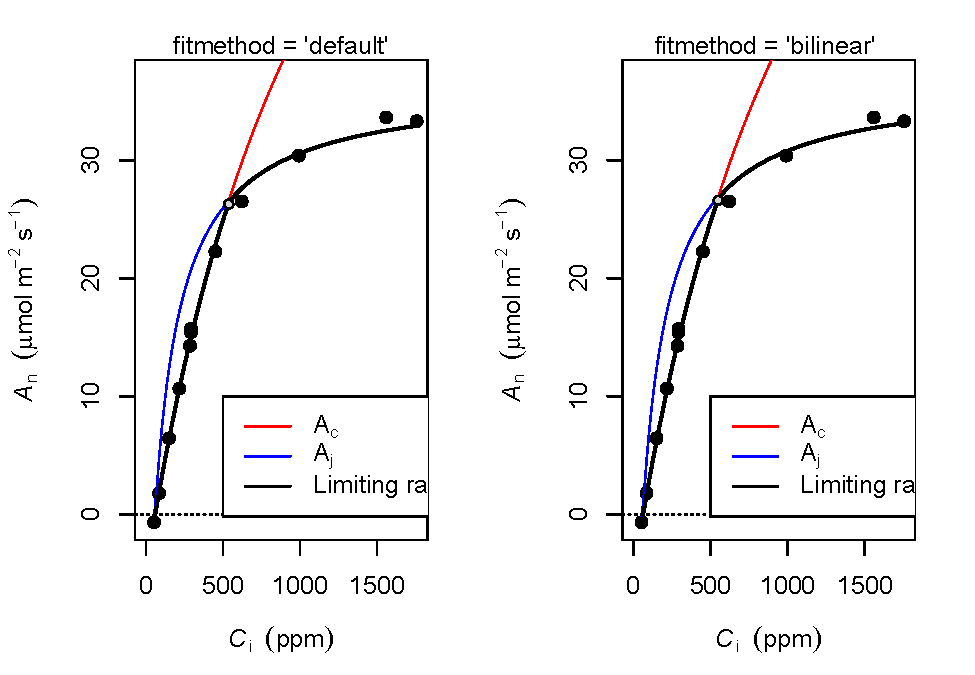
\includegraphics{bookdown_files/figure-latex/fitaci6400-1.pdf}
\caption{\label{fig:fitaci6400}光合速率的不同的限制阶段}
\end{figure}

如果需要导出数据做他用,直接根据 \texttt{attributes} 中看到的名称,选择对应的数据导出即可,如果使用 Rstudio 的话,其自动补全的功能在选择数据上更方便。例如导出预测值和系数分别使用如下方式:

\begin{Shaded}
\begin{Highlighting}[]
\CommentTok{# 将模型拟合结果中df(即计算数据)赋给predictaci,}
\CommentTok{# 并用write.csv导出}
\NormalTok{predictaci <-}\StringTok{ }\NormalTok{acifit}\OperatorTok{$}\NormalTok{df}
\KeywordTok{write.csv}\NormalTok{(acifit}\OperatorTok{$}\NormalTok{df, }\DataTypeTok{file =} \StringTok{"acipredict.csv"}\NormalTok{)}
\KeywordTok{write.csv}\NormalTok{(}\KeywordTok{coef}\NormalTok{(acifit), }\DataTypeTok{file =} \StringTok{"coefaci.csv"}\NormalTok{)}
\end{Highlighting}
\end{Shaded}

\begin{quote}
需要注意的是,因为非线性拟合需要一个初始值,因此,使用默认方式(非线性拟合)的时候,会存在可能的拟合失败现象,此时可以使用 \texttt{fitmethod\ =\ "bilinear"},二者结果略有差别。
\end{quote}

\hypertarget{onepoint}{%
\subsubsection{fitmethod = ``onepoint'' 介绍}\label{onepoint}}

\citet{De2016A} 发表了关于 one point 方法计算 \(V_{cmax}\) 和 \(J_{max}\) 方法的文章,在 2017 年 11 月的更新中,plantecophys 增加了响应的 R 软件实现方法, 该方法并非使用一个点计算 \(V_{cmax}\) 和 \(J_{max}\),而是对数据集中的每一个点的值进行估计,使用的方法为逆向了光合作用方程。输出为对每个原始数据加入了 \(V_{cmax}\) 和 \(J_{max}\),当然一如既往的可以使用温度校准的方法。\textbf{并不建议该方法应用于整个 ACi 曲线的数据,它的假设是在外部环境 CO\textsubscript{2} 浓度和饱和光下,受到 Rubisco 羧化速率的限制而不是 RUBP 的限制。}

基于上面的描述,他们的模型如下:

\begin{equation}
\hat{V}_{cmax} = (A_{sat} + R_{day}) \frac{C_i + K_m}{C_i - \Gamma^*} 
\label{eq:inverseA}
\end{equation}

其中:K\textsubscript{m} 为米氏常数,其计算为:

\begin{equation}
K_m = K_c (1 + \frac{O_i}{K_o}) 
\label{eq:km}
\end{equation}

未知参数均由文献中的方法进行计算,具体可参考 \citet{De2016A} 的原文,但上述方法的缺陷为还要使用 ACi 曲线来估算 R\textsubscript{day},因此作者使用了1.5\% V\textsubscript{cmax} 作为 R\textsubscript{day},因此公式 \eqref{eq:inverseA} 可变换为:

\begin{equation}
\hat{V}_{cmax} = A_{sat} (\frac{C_i + K_m}{C_i - \Gamma^*} - 0.015)
\label{eq:onepoint}
\end{equation}

另一个重要的模型的假设为 J\textsubscript{max} 与 V\textsubscript{cmax} 是成比例的, J\textsubscript{max} 的计算是通过 C\textsubscript{i} transition point 来实现的,文章中的比值均值为 1.9,范围在 1.68 \textasciitilde{} 2.14 之间。

\hypertarget{onpoint_fit}{%
\subsection{\texorpdfstring{使用 `onepoint' 单独计算 V\textsubscript{cmax} 和 J\textsubscript{max}}{使用 `onepoint' 单独计算 Vcmax 和 Jmax}}\label{onpoint_fit}}

目前我手头没有相应数据,仅有使用 LI-6400 测试 auto log 2 时的一个数据,我们用这个来示范该方法的使用:

\begin{Shaded}
\begin{Highlighting}[]
\NormalTok{one_data <-}\StringTok{ }\KeywordTok{read.csv}\NormalTok{(}\StringTok{"./data/onepoint.csv"}\NormalTok{)}
\NormalTok{knitr}\OperatorTok{::}\KeywordTok{kable}\NormalTok{(}\KeywordTok{head}\NormalTok{(one_data), }\DataTypeTok{booktabs =} \OtherTok{TRUE}\NormalTok{,}
             \DataTypeTok{caption =} \StringTok{'onepoint 使用的数据'}\NormalTok{)}
\end{Highlighting}
\end{Shaded}

\begin{table}[t]

\caption{\label{tab:onepointdata}onepoint 使用的数据}
\centering
\begin{tabular}{rlrrrrrrrrrrrrrrrrrrrrrrrrrrrrrrrrrrrrrrrrrrrrrrrrrrrrrrrrrr}
\toprule
Obs & HHMMSS & FTime & EBal. & Photo & Cond & Ci & Trmmol & VpdL & CTleaf & Area & BLC\_1 & StmRat & BLCond & Tair & Tleaf & TBlk & CO2R & CO2S & H2OR & H2OS & RH\_R & RH\_S & Flow & PARi & PARo & Press & CsMch & HsMch & CsMchSD & HsMchSD & CrMchSD & HrMchSD & StableF & BLCslope & BLCoffst & f\_parin & f\_parout & alphaK & Status & fda & Trans & Tair\_K & Twall\_K & R.W.m2. & Tl.Ta & SVTleaf & h2o\_i & h20diff & CTair & SVTair & CndTotal & vp\_kPa & VpdA & CndCO2 & Ci\_Pa & Ci.Ca & RHsfc & C2sfc & AHs.Cs\\
\midrule
1 & 14:12:43 & 347.0 & 0 & 10.519216 & 0.1369336 & 263.0905 & 1.963046 & 1.445782 & 25.89411 & 6 & 1.42 & 1 & 2.84 & 25.86572 & 25.89411 & 25.86697 & 412.5374 & 398.9832 & 16.98853 & 19.29724 & 50.16200 & 56.97891 & 500.3231 & 1198.761 & 7.497697 & 98.84273 & 2.011996 & -0.3824501 & 0.1618589 & 0.0039255 & 0.1864786 & 0.0030409 & 1.0000000 & -0.2195652 & 2.737392 & 1 & 0 & 0.16 & 111115 & 0.8338718 & 0.0019630 & 299.0441 & 299.0157 & 191.8018 & 1.191025 & 3.353173 & 33.92433 & 14.62709 & 25.87991 & 3.350355 & 0.1306349 & 1.907392 & 1.442964 & 0.0821903 & 26.00458 & 0.6594024 & 57.74196 & 393.9829 & 0.0154169\\
2 & 14:13:04 & 369.0 & 0 & 10.361122 & 0.1357092 & 264.1135 & 1.946022 & 1.445559 & 25.89542 & 6 & 1.42 & 1 & 2.84 & 25.86854 & 25.89542 & 25.86977 & 412.5459 & 399.1890 & 17.01363 & 19.30231 & 50.22723 & 56.98380 & 500.3223 & 1198.748 & 7.486364 & 98.84175 & 2.018435 & -0.3787848 & 0.2174792 & 0.0025482 & 0.2455426 & 0.0025012 & 1.0000000 & -0.2195652 & 2.737392 & 1 & 0 & 0.16 & 111115 & 0.8338705 & 0.0019460 & 299.0454 & 299.0185 & 191.7997 & 1.199722 & 3.353433 & 33.92729 & 14.62498 & 25.88198 & 3.350765 & 0.1295200 & 1.907874 & 1.442891 & 0.0814842 & 26.10544 & 0.6616252 & 57.73418 & 394.2638 & 0.0151724\\
3 & 14:13:25 & 373.0 & 0 & 10.207166 & 0.1342114 & 264.8348 & 1.925734 & 1.445717 & 25.89660 & 6 & 1.42 & 1 & 2.84 & 25.87186 & 25.89660 & 25.87317 & 412.5393 & 399.3762 & 17.03833 & 19.30316 & 50.29006 & 56.97489 & 500.3188 & 1198.737 & 7.489428 & 98.84142 & 2.018435 & -0.3787848 & 0.2174792 & 0.0025482 & 0.2455426 & 0.0025012 & 1.0000000 & -0.2195652 & 2.737392 & 1 & 0 & 0.16 & 111115 & 0.8338647 & 0.0019257 & 299.0466 & 299.0219 & 191.7980 & 1.210137 & 3.353668 & 33.92979 & 14.62663 & 25.88423 & 3.351212 & 0.1281551 & 1.907951 & 1.443261 & 0.0806199 & 26.17665 & 0.6631213 & 57.71117 & 394.5242 & 0.0149311\\
4 & 14:13:41 & 389.5 & 0 & 9.547416 & 0.1281947 & 269.6337 & 1.854272 & 1.454248 & 25.94020 & 6 & 1.42 & 1 & 2.84 & 25.91845 & 25.94020 & 25.92104 & 413.8090 & 401.4666 & 17.12559 & 19.30638 & 50.40359 & 56.82203 & 500.3162 & 1199.245 & 7.449210 & 98.83208 & 2.018435 & -0.3787848 & 0.2174792 & 0.0025482 & 0.2455426 & 0.0025012 & 1.0000000 & -0.2195652 & 2.737392 & 1 & 0 & 0.16 & 111115 & 0.8338604 & 0.0018543 & 299.0902 & 299.0684 & 191.8792 & 1.247158 & 3.362337 & 34.02071 & 14.71433 & 25.92933 & 3.360173 & 0.1226580 & 1.908089 & 1.452084 & 0.0771402 & 26.64846 & 0.6716216 & 57.48324 & 396.9282 & 0.0138266\\
5 & 14:16:16 & 540.0 & 0 & 10.288968 & 0.1376602 & 267.9198 & 2.009217 & 1.471788 & 26.01813 & 6 & 1.42 & 1 & 2.84 & 26.01478 & 26.01813 & 26.02164 & 413.9044 & 400.5999 & 16.92567 & 19.28878 & 49.53554 & 56.44850 & 500.3043 & 1200.785 & 7.497018 & 98.81870 & 2.018435 & -0.3787848 & 0.2174792 & 0.0025482 & 0.2455426 & 0.0025012 & 0.6666667 & -0.2195652 & 2.737392 & 1 & 0 & 0.16 & 111115 & 0.8338405 & 0.0020092 & 299.1681 & 299.1648 & 192.1257 & 1.174669 & 3.377880 & 34.18260 & 14.89382 & 26.01646 & 3.377546 & 0.1312960 & 1.906093 & 1.471453 & 0.0826090 & 26.47549 & 0.6687965 & 57.30143 & 395.7090 & 0.0148991\\
\addlinespace
6 & 14:16:32 & 555.5 & 0 & 10.178603 & 0.1381995 & 269.5898 & 2.016100 & 1.471138 & 26.01657 & 6 & 1.42 & 1 & 2.84 & 26.02212 & 26.01657 & 26.02939 & 413.6639 & 400.4885 & 16.92345 & 19.29468 & 49.49181 & 56.42595 & 500.2979 & 1200.879 & 7.569045 & 98.80596 & 2.018435 & -0.3787848 & 0.2174792 & 0.0025482 & 0.2455426 & 0.0025012 & 0.6666667 & -0.2195652 & 2.737392 & 1 & 0 & 0.16 & 111115 & 0.8338298 & 0.0020161 & 299.1666 & 299.1721 & 192.1406 & 1.172561 & 3.377567 & 34.18384 & 14.88916 & 26.01934 & 3.378122 & 0.1317865 & 1.906429 & 1.471693 & 0.0829197 & 26.63708 & 0.6731525 & 57.32389 & 395.6501 & 0.0147473\\
\bottomrule
\end{tabular}
\end{table}

数据如上所示,为同一个叶片连续记录数据,故所有的光合速率十分接近。

使用方法:

\begin{Shaded}
\begin{Highlighting}[]
\KeywordTok{library}\NormalTok{(plantecophys)}

\NormalTok{one_data <-}\StringTok{ }\KeywordTok{subset}\NormalTok{(one_data, Obs }\OperatorTok{>}\StringTok{ }\DecValTok{0}\NormalTok{)}
\NormalTok{one_data}\OperatorTok{$}\NormalTok{Rd <-}\StringTok{ }\KeywordTok{rep}\NormalTok{(}\OperatorTok{-}\FloatTok{0.5}\NormalTok{, }\KeywordTok{length}\NormalTok{(one_data}\OperatorTok{$}\NormalTok{Obs))}
\NormalTok{aci_fit <-}\StringTok{ }\KeywordTok{fitaci}\NormalTok{(one_data, }\DataTypeTok{fitmethod =} \StringTok{"onepoint"}\NormalTok{)}

\NormalTok{knitr}\OperatorTok{::}\KeywordTok{kable}\NormalTok{(}\KeywordTok{head}\NormalTok{(}\KeywordTok{data.frame}\NormalTok{(aci_fit}\OperatorTok{$}\NormalTok{Photo, }
\NormalTok{             aci_fit}\OperatorTok{$}\NormalTok{Vcmax, aci_fit}\OperatorTok{$}\NormalTok{Jmax)),}
             \DataTypeTok{booktabs =} \OtherTok{TRUE}\NormalTok{,}
             \DataTypeTok{caption =} \StringTok{'onepoint 法计算的结果'}\NormalTok{)}
\end{Highlighting}
\end{Shaded}

\begin{table}[t]

\caption{\label{tab:onepoint}onepoint 法计算的结果}
\centering
\begin{tabular}{rrr}
\toprule
aci\_fit.Photo & aci\_fit.Vcmax & aci\_fit.Jmax\\
\midrule
10.519216 & 47.06893 & 71.73759\\
10.361122 & 46.22091 & 70.51059\\
10.207166 & 45.44617 & 69.35838\\
9.547416 & 41.86217 & 64.24400\\
10.288968 & 45.09335 & 69.36954\\
\addlinespace
10.178603 & 44.37360 & 68.41628\\
\bottomrule
\end{tabular}
\end{table}

需要注意,为保证结果的精确,如果不设定 Rd, 也即文献中的 Rday, 模型是无法计算的,因此上面的示例中虚构了一个,实际操作用一般使用标准的 ACi 测量计算。

\hypertarget{multi_curve}{%
\subsection{\texorpdfstring{多条 CO\textsubscript{2} 响应曲线的拟合}{多条 CO2 响应曲线的拟合}}\label{multi_curve}}

fitacis 函数实际上是 fitaci 函数的扩展,方便一次拟合多条曲线\footnote{需要注意,此时fitmethod一般推荐使用bilinear。}。函数的参数如下:

\begin{Shaded}
\begin{Highlighting}[]
\KeywordTok{fitacis}\NormalTok{(data, group, }\DataTypeTok{fitmethod =} \KeywordTok{c}\NormalTok{(}\StringTok{"default"}\NormalTok{, }
        \StringTok{"bilinear"}\NormalTok{),}\DataTypeTok{progressbar =} \OtherTok{TRUE}\NormalTok{, }
        \DataTypeTok{quiet =} \OtherTok{FALSE}\NormalTok{, }\DataTypeTok{id =} \OtherTok{NULL}\NormalTok{, ...)}

\CommentTok{## S3 method for class 'acifits'}
\KeywordTok{plot}\NormalTok{(x, }\DataTypeTok{how =} \KeywordTok{c}\NormalTok{(}\StringTok{"manyplots"}\NormalTok{, }\StringTok{"oneplot"}\NormalTok{), }
     \DataTypeTok{highlight =} \OtherTok{NULL}\NormalTok{, }\DataTypeTok{ylim =} \OtherTok{NULL}\NormalTok{, }
     \DataTypeTok{xlim =} \OtherTok{NULL}\NormalTok{, }\DataTypeTok{add =} \OtherTok{FALSE}\NormalTok{, }\DataTypeTok{what =} \KeywordTok{c}\NormalTok{(}\StringTok{"model"}\NormalTok{,}
     \StringTok{"data"}\NormalTok{, }\StringTok{"none"}\NormalTok{), ...)}
\end{Highlighting}
\end{Shaded}

\textbf{主要参数详解:}

实际上 fitacis 与 fitaci 模型算法完全一致,只不过增加了一个 group 参数,用于区分不同测量的数据,具体请参考举例内容。

\hypertarget{fitacis_exa}{%
\subsubsection{fitacis 函数应用举例}\label{fitacis_exa}}

下文代码根据 plantecophys 中的示例代码修改,进行演示,原代码请参考其帮助文档。

\begin{Shaded}
\begin{Highlighting}[]
\KeywordTok{library}\NormalTok{(plantecophys)}
\CommentTok{# 只提取前10个不同测量的数据,节省时间进行举例}
\NormalTok{manyacidat2 <-}\StringTok{ }\KeywordTok{droplevels}\NormalTok{(manyacidat[manyacidat}\OperatorTok{$}\NormalTok{Curve }\OperatorTok\StringTok{ }
\StringTok{                                       }\KeywordTok{levels}\NormalTok{(manyacidat}\OperatorTok{$}\NormalTok{Curve)[}\DecValTok{1}\OperatorTok{:}\DecValTok{10}\NormalTok{],])}

\CommentTok{# 对多条曲线进行拟合,使用bilinear方法,}
\CommentTok{# 仅仅因为其比非线性拟合节省时间}
\NormalTok{fits <-}\StringTok{ }\KeywordTok{fitacis}\NormalTok{(manyacidat2, }\DataTypeTok{group =} \StringTok{"Curve"}\NormalTok{, }\DataTypeTok{fitmethod=}\StringTok{"bilinear"}\NormalTok{, }\DataTypeTok{quiet =} \OtherTok{TRUE}\NormalTok{)}

\CommentTok{# 拟合结果为list,我们可以只提取第一个的拟合结果}
\NormalTok{fits[[}\DecValTok{1}\NormalTok{]]}
\end{Highlighting}
\end{Shaded}

\begin{verbatim}
## Result of fitaci.
## 
## Data and predictions:
##            Ci      Ameas     Amodel         Ac        Aj   Ap        Rd
## 2    53.23129 -0.4401082  0.1014381  0.9601119  2.548123 1000 0.8586158
## 3    79.47367  2.4824630  2.1937702  3.0526198  7.036734 1000 0.8586158
## 4   116.74688  5.4531712  4.9419337  5.8011511 11.392394 1000 0.8586158
## 5   188.00801  9.7099879  9.5705964 10.4310194 16.447715 1000 0.8586158
## 6   278.44662 14.8225766 14.4261545 15.2897486 19.977583 1000 0.8586158
## 7   343.03259 17.7982155 17.4602014 18.3289218 21.639847 1000 0.8586158
## 1   344.72152 17.9244012 17.3165146 18.1849643 21.534276 1000 0.8586158
## 14  344.74839 16.7933747 17.6853306 18.5545917 21.774261 1000 0.8586158
## 8   588.08078 23.8925326 24.1309683 27.0327638 25.020148 3000 0.8586158
## 9   833.25547 26.5674409 25.7783026 33.0856065 26.647921 3000 0.8586158
## 10 1136.99222 25.9787890 26.8108335 38.1296944 27.676768 3000 0.8586158
## 11 1436.86370 26.6110657 27.5409345 42.0628463 28.405453 3000 0.8586158
## 12 1536.46772 27.4018784 27.7965881 43.3773689 28.660781 3000 0.8586158
## 13 1731.76400 28.6752069 28.0952804 45.2475932 28.959041 3000 0.8586158
##    VPD    Tleaf         Cc     PPFD Patm Ci_original
## 2  1.5 24.55873   53.23139 1799.959  100    53.23129
## 3  1.5 24.58292   79.47586 1799.590  100    79.47367
## 4  1.5 24.71278  116.75183 1799.819  100   116.74688
## 5  1.5 24.73687  188.01759 1800.371  100   188.00801
## 6  1.5 24.67508  278.46106 1800.233  100   278.44662
## 7  1.5 24.76596  343.05006 1799.575  100   343.03259
## 1  1.5 24.51593  344.73886 1800.356  100   344.72152
## 14 1.5 24.94098  344.76609 1799.964  100   344.74839
## 8  1.5 24.83785  588.10494 1799.477  100   588.08078
## 9  1.5 24.91185  833.28127 1799.969  100   833.25547
## 10 1.5 24.87314 1137.01906 1799.525  100  1136.99222
## 11 1.5 24.95914 1436.89126 1799.615  100  1436.86370
## 12 1.5 25.04542 1536.49554 1799.784  100  1536.46772
## 13 1.5 25.07566 1731.79212 1799.160  100  1731.76400
## 
## Root mean squared error:  2.196037 
## 
## Estimated parameters:
##          Estimate Std. Error
## Vcmax  65.0009909  1.3720635
## Jmax  131.7980133         NA
## Rd      0.8586158  0.2876248
## Note: Vcmax, Jmax are at 25C, Rd is at measurement T.
## 
## Curve was fit using method:  bilinear 
## 
## Parameter settings:
## Patm = 100
##  alpha = 0.24
##  theta = 0.85
##  EaV = 82620.87
##  EdVC = 0
##  delsC = 645.1013
##  EaJ = 39676.89
##  EdVJ = 2e+05
##  delsJ = 641.3615
## 
## Estimated from Tleaf (shown at mean Tleaf):
## GammaStar =  42.31453 
## Km =  698.2084
\end{verbatim}

\begin{Shaded}
\begin{Highlighting}[]
\CommentTok{# 使用sapply提取拟合结果的RMSE(均方根误差)}
\NormalTok{rmses <-}\StringTok{ }\KeywordTok{sapply}\NormalTok{(fits, }\StringTok{"[["}\NormalTok{, }\StringTok{"RMSE"}\NormalTok{)}
\KeywordTok{plot}\NormalTok{(rmses, }\DataTypeTok{type=}\StringTok{'h'}\NormalTok{, }\DataTypeTok{ylab=}\StringTok{"RMSE"}\NormalTok{, }\DataTypeTok{xlab=}\StringTok{"Curve nr"}\NormalTok{)}
\end{Highlighting}
\end{Shaded}

\begin{figure}
\centering
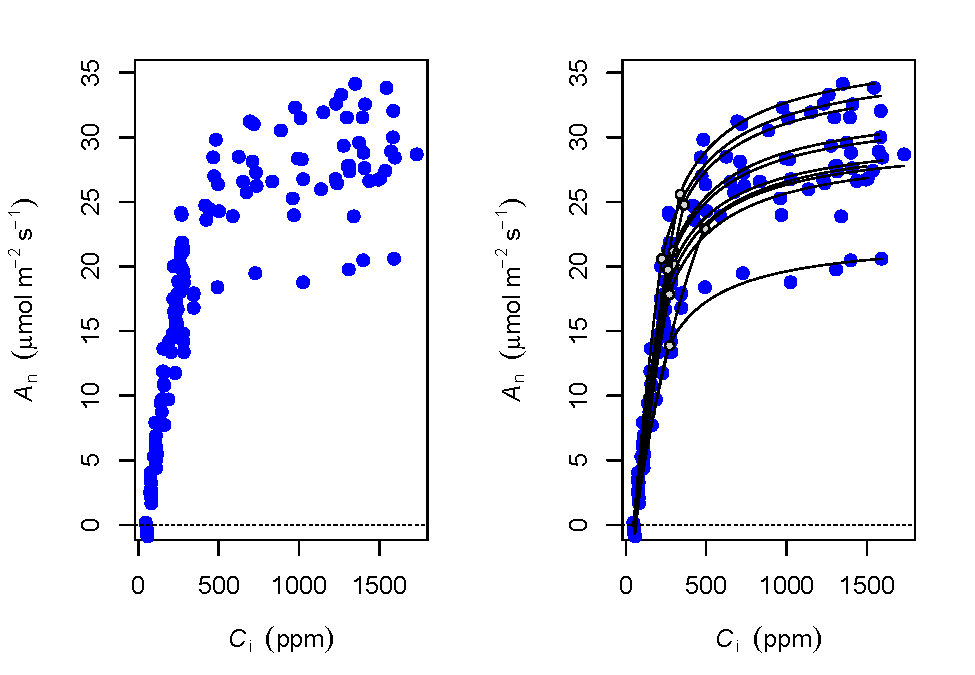
\includegraphics{bookdown_files/figure-latex/fitacisr-1.pdf}
\caption{\label{fig:fitacisr1}fitacis作图结果}
\end{figure}

\begin{Shaded}
\begin{Highlighting}[]
\CommentTok{# 对最差的拟合结果进行作图}
\KeywordTok{plot}\NormalTok{(fits[[}\KeywordTok{which.max}\NormalTok{(rmses)]])}
\end{Highlighting}
\end{Shaded}

\begin{figure}
\centering
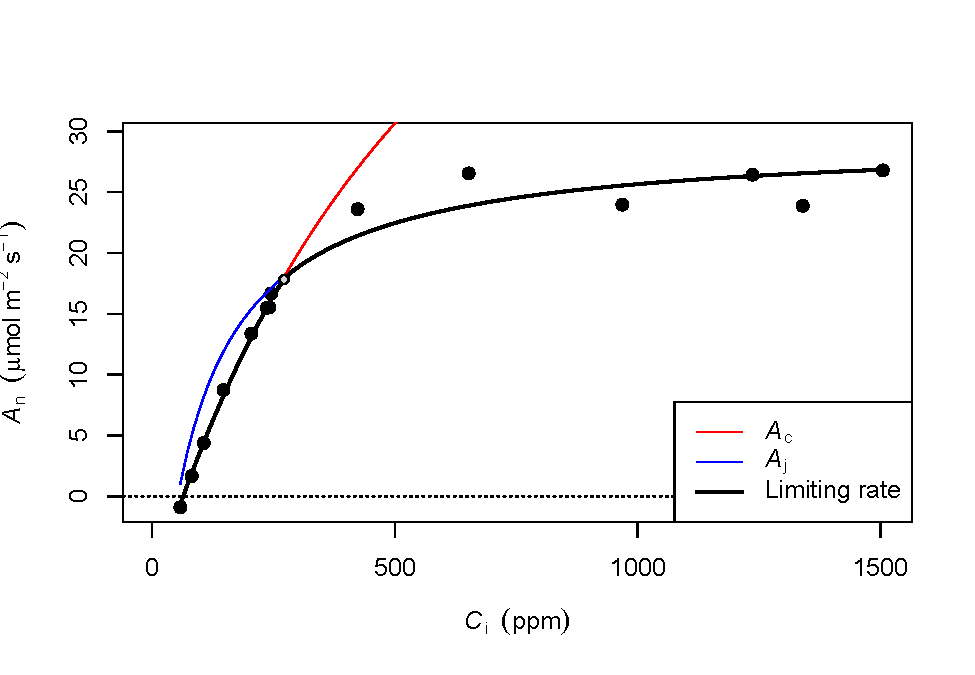
\includegraphics{bookdown_files/figure-latex/fitacisr-2.pdf}
\caption{\label{fig:fitacisr2}fitacis作图结果}
\end{figure}

可以看出,\texttt{fitaci} 和 \texttt{fitacis} 用法基本一致,各行代码均已经注释,更详细用法请参函数考帮助。

\hypertarget{transition}{%
\subsection{\texorpdfstring{\texttt{findCiTransition} 函数}{findCiTransition 函数}}\label{transition}}

计算 CiTransition 的函数,第一点为 Ac \& Aj,第二点为 Aj \& Ap,并且仅在计算 TPU 的前提下才会有第二点出现。

\begin{Shaded}
\begin{Highlighting}[]
\KeywordTok{findCiTransition}\NormalTok{(object, ...)}
\end{Highlighting}
\end{Shaded}

参数使用,object 为 fitaci 函数对象,或者整个的 \texttt{Photosyn} 函数。
\ldots{} 为使用 \texttt{Photosyn} 时可传递的参数。

\hypertarget{c4}{%
\section{C4 植物光合}\label{c4}}

之前的部分模型全部为关于 C3 植物的拟合,而 \citet{Caemmerer2000Biochemical} 的方法,则是针对
C4 植物的 A-Ci 曲线的实现。

\begin{Shaded}
\begin{Highlighting}[]
\KeywordTok{AciC4}\NormalTok{(Ci, }\DataTypeTok{PPFD =} \DecValTok{1500}\NormalTok{, }\DataTypeTok{Tleaf =} \DecValTok{25}\NormalTok{, }\DataTypeTok{VPMAX25 =} \DecValTok{120}\NormalTok{, }
      \DataTypeTok{JMAX25 =} \DecValTok{400}\NormalTok{, }\DataTypeTok{Vcmax =} \DecValTok{60}\NormalTok{, }\DataTypeTok{Vpr =} \DecValTok{80}\NormalTok{, }
      \DataTypeTok{alpha =} \DecValTok{0}\NormalTok{, }\DataTypeTok{gbs =} \FloatTok{0.003}\NormalTok{, }\DataTypeTok{O2 =} \DecValTok{210}\NormalTok{, }
      \DataTypeTok{x =} \FloatTok{0.4}\NormalTok{, }\DataTypeTok{THETA =} \FloatTok{0.7}\NormalTok{, }\DataTypeTok{Q10 =} \FloatTok{2.3}\NormalTok{, }
      \DataTypeTok{RD0 =} \DecValTok{1}\NormalTok{, }\DataTypeTok{RTEMP =} \DecValTok{25}\NormalTok{, }\DataTypeTok{TBELOW =} \DecValTok{0}\NormalTok{, }
      \DataTypeTok{DAYRESP =} \DecValTok{1}\NormalTok{, }\DataTypeTok{Q10F =} \DecValTok{2}\NormalTok{, }\DataTypeTok{FRM =} \FloatTok{0.5}\NormalTok{, ...)}
\end{Highlighting}
\end{Shaded}

\textbf{参数详解}

\begin{itemize}
\tightlist
\item
  Ci:胞间二氧化碳浓度 (\(\mu mol\cdot m^{-2}\cdot s^{-1}\))。
\item
  PPFD:光合光量子通量密度 (\(\mu mol\cdot m^{-2}\cdot s^{-1}\))。
\item
  Tleaf:叶片温度 (\textcelsius)。
\item
  VPMAX25:PEP 羧化最大速率 (\(\mu mol\cdot m^{-2}\cdot s^{-1}\))。
\item
  JMAX25:最大电子传递速率 (\textcelsius))。
\item
  Vcmax:最大羧化速率(\(\mu mol\cdot m^{-2}\cdot s^{-1}\))。
\item
  Vpr:PEP 再生(\(\mu mol\cdot m^{-2}\cdot s^{-1}\))。
\item
  alpha:维管束鞘细胞中 PSII 活性的比例。
\item
  gbs:维管束鞘导度 (\(mol\cdot m^{-2}\cdot s^{-1}\))。
\item
  O2:叶肉细胞氧气浓度。
\item
  x:电子传递的分配因子。
\item
  THETA:曲角参数。
\item
  Q10:Michaelis-Menten 系数中依赖于温度的参数。
\item
  RD0:基温下的呼吸 (\(mol\cdot m^{-2}\cdot s^{-1}\))。
\item
  RTEMP:呼吸的基温(\textcelsius)
\item
  TBELOW:此温度以下呼吸为0。
\item
  DAYRESP:明呼吸和暗呼吸的比值。
\item
  Q10F:呼吸依赖于温度的参数。
\item
  FRM:明呼吸中为叶肉呼吸的比例。
\end{itemize}

以上参数均来自 \citet{Caemmerer2000Biochemical},括号中的参数值均为默认值,具体应用时请按照实际情况修改。

\hypertarget{c4_sim}{%
\subsection{C4 植物光合速率的计算}\label{c4_sim}}

\begin{Shaded}
\begin{Highlighting}[]
\CommentTok{# 模拟 C4 植物的 Ci 值,计算光合速率并作图}
\KeywordTok{library}\NormalTok{(plantecophys)}
\NormalTok{aci <-}\StringTok{ }\KeywordTok{AciC4}\NormalTok{(}\DataTypeTok{Ci=}\KeywordTok{seq}\NormalTok{(}\DecValTok{5}\NormalTok{,}\DecValTok{600}\NormalTok{, }\DataTypeTok{length=}\DecValTok{101}\NormalTok{))}
\KeywordTok{with}\NormalTok{(aci, }\KeywordTok{plot}\NormalTok{(Ci, ALEAF, }\DataTypeTok{type=}\StringTok{'l'}\NormalTok{, }\DataTypeTok{ylim=}\KeywordTok{c}\NormalTok{(}\DecValTok{0}\NormalTok{,}\KeywordTok{max}\NormalTok{(ALEAF))))}
\end{Highlighting}
\end{Shaded}

\begin{figure}
\centering
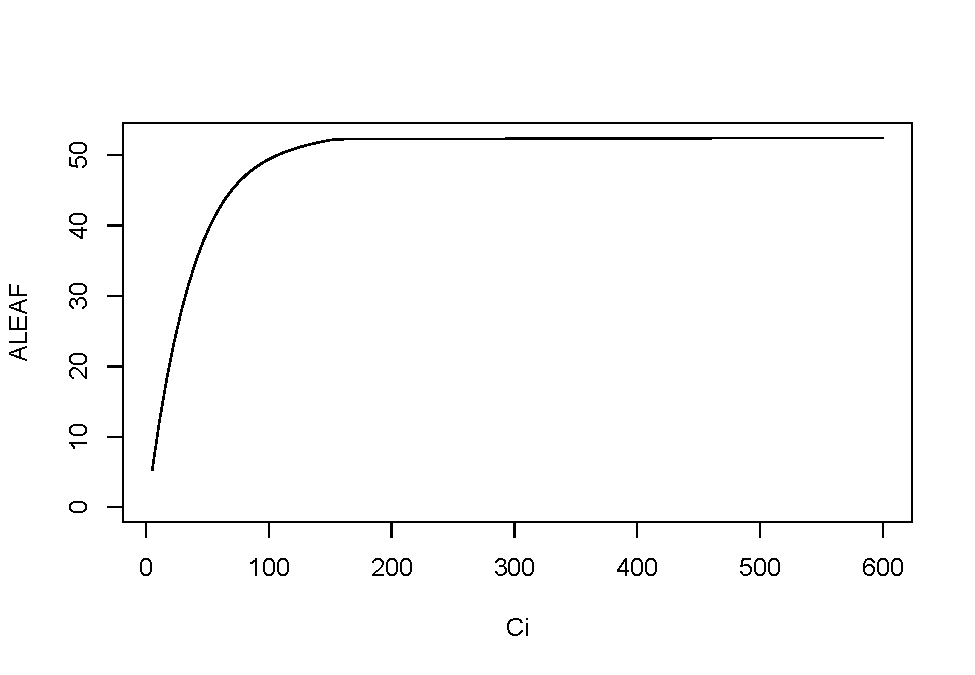
\includegraphics{bookdown_files/figure-latex/unnamed-chunk-17-1.pdf}
\caption{\label{fig:unnamed-chunk-17}C4 植物 A-Ci 作图}
\end{figure}

\cleardoublepage

\hypertarget{stomotal_sim}{%
\chapter{气孔导度模型的拟合}\label{stomotal_sim}}

气孔导度模型的拟合是通过 \texttt{fitBB} 来实现的,可以拟合三个 \textbf{Ball-Berry 类型的气孔导度模型},共有下面几个参数:

\begin{itemize}
\tightlist
\item
  气孔导度 (gs),
\item
  光合 (A),
\item
  外界 CO\textsubscript{2} 浓度 (Ca)
\item
  水气压亏缺 (VPD).
\end{itemize}

其三个模型的简介如下:

\hypertarget{ballberry}{%
\section{BallBerry 模型}\label{ballberry}}

\citet{Ball1987A} 发表的文章中的模型:

\begin{equation}
g_s = g0 + g1(\frac{A h_r}{C_a})
\label{eq:ballberry}
\end{equation}

其中 A 为净光合速率,g\textsubscript{0} 和 g\textsubscript{1} 为拟合参数,h\textsubscript{r} 为叶片表面的相对湿度,C\textsubscript{a} 为叶片处CO\textsubscript{2}浓度。

\hypertarget{bbleuning}{%
\section{BBLeuning 模型}\label{bbleuning}}

\citet{leuning1995a} 发表的文章中的模型:

\begin{equation}
g_s = g_0 + g_1(\frac{A}{(C_a - \Gamma)(1 + \frac{D}{D_0})})
\label{eq:BBLeuning}
\end{equation}

其中 \(\Gamma\) 为 CO\textsubscript{2} 补偿点,g\textsubscript{0}、g\textsubscript{1} 和 D\textsubscript{0} 为拟合参数。

\hypertarget{bboptifull}{%
\section{BBOptiFull 模型}\label{bboptifull}}

\citet{Medlyn2011Reconciling} 发表的文章中的模型:

\begin{equation}
g_s^* \approx g_0 + g_1(1 + \frac{g_1}{D}) \frac{A}{C_a}
\label{eq:BBOptiFull}
\end{equation}

额外的参数 g\textsubscript{k} 来自于 \citet{Duursma2013Near}
\begin{equation}
g_s = g_0 + 1.6(1 + \frac{g_1}{D}(1-g_k)) \frac{A}{C_a}
\label{eq:Duursm}
\end{equation}

\hypertarget{fitbb-p}{%
\section{\texorpdfstring{\texttt{fitBB} 函数}{fitBB 函数}}\label{fitbb-p}}

\begin{Shaded}
\begin{Highlighting}[]
\KeywordTok{fitBB}\NormalTok{(data, }\DataTypeTok{varnames =} \KeywordTok{list}\NormalTok{(}
  \DataTypeTok{ALEAF =} \StringTok{"A"}\NormalTok{, }\DataTypeTok{GS =} \StringTok{"gsw"}\NormalTok{, }\DataTypeTok{VPD =} \StringTok{"VPDleaf"}\NormalTok{,}
  \DataTypeTok{Ca =}\StringTok{"CO2_s"}\NormalTok{, }\DataTypeTok{RH =} \StringTok{"RHcham"}\NormalTok{), }
  \DataTypeTok{gsmodel =} \KeywordTok{c}\NormalTok{(}\StringTok{"BBOpti"}\NormalTok{, }\StringTok{"BBLeuning"}\NormalTok{, }\StringTok{"BallBerry"}\NormalTok{,}
              \StringTok{"BBOptiFull"}\NormalTok{), }\DataTypeTok{fitg0 =} \OtherTok{FALSE}\NormalTok{)}
\end{Highlighting}
\end{Shaded}

\textbf{参数的意义:}

\begin{itemize}
\tightlist
\item
  data:待分析的数据文件。
\item
  varnames:注意,函数默认数据为 6400 格式,因此 6800 的数据文件要安装上文的参数修改。 相对湿度只有在使用 BallBerry 时才需要输入。
\item
  gsmodel:上述三个模型之一。
\item
  fitg0:默认不计算g0,若需要,改为TRUE。
\end{itemize}

\textbf{代码示例:}

\begin{Shaded}
\begin{Highlighting}[]
\KeywordTok{library}\NormalTok{(plantecophys)}

\NormalTok{aci <-}\StringTok{ }\KeywordTok{read.csv}\NormalTok{(}\StringTok{"./data/aci.csv"}\NormalTok{)}
\NormalTok{aci <-}\StringTok{ }\KeywordTok{subset}\NormalTok{(aci, Obs }\OperatorTok{>}\StringTok{ }\DecValTok{0}\NormalTok{)}
\KeywordTok{fitBB}\NormalTok{(aci, }\DataTypeTok{varnames =} \KeywordTok{list}\NormalTok{(}\DataTypeTok{ALEAF =} \StringTok{"Photo"}\NormalTok{, }\DataTypeTok{GS =} \StringTok{"Cond"}\NormalTok{, }\DataTypeTok{VPD =} \StringTok{"VpdL"}\NormalTok{,}
  \DataTypeTok{Ca =} \StringTok{"CO2S"}\NormalTok{, }\DataTypeTok{RH =} \StringTok{"RH_S"}\NormalTok{), }\DataTypeTok{gsmodel =} \StringTok{"BBOpti"}\NormalTok{, }\DataTypeTok{fitg0 =} \OtherTok{TRUE}\NormalTok{)}
\end{Highlighting}
\end{Shaded}

\begin{verbatim}
## Result of fitBB.
## Model :  BBOpti 
## Both g0 and g1 were estimated.
## 
## Coefficients:
## g0  g1
## 0.326 -0.992 
## 
## For more details of the fit, look at summary(myfit$fit)
## To return coefficients, do coef(myfit).
## (where myfit is the name of the object returned by fitBB)
\end{verbatim}

\hypertarget{fitbbs}{%
\section{\texorpdfstring{\texttt{fitBBs} 函数}{fitBBs 函数}}\label{fitbbs}}

如果我们有多个物种的数据,那么使用 \texttt{fitBBs} 则可以快速拟合多条曲线的数据。我们先整合两次的数据,然后再查看运行结果:

\begin{Shaded}
\begin{Highlighting}[]
\NormalTok{aci01 <-}\StringTok{ }\KeywordTok{read.csv}\NormalTok{(}\StringTok{"./data/aci01.csv"}\NormalTok{)}
\NormalTok{aci01 <-}\StringTok{ }\KeywordTok{subset}\NormalTok{(aci01, Obs }\OperatorTok{>}\StringTok{ }\DecValTok{0}\NormalTok{)}
\NormalTok{multiBB <-}\StringTok{ }\KeywordTok{data.frame}\NormalTok{(}
  \DataTypeTok{A =} \KeywordTok{c}\NormalTok{(aci}\OperatorTok{$}\NormalTok{Photo, aci01}\OperatorTok{$}\NormalTok{Photo),}
  \DataTypeTok{GS =} \KeywordTok{c}\NormalTok{(aci}\OperatorTok{$}\NormalTok{Cond, aci01}\OperatorTok{$}\NormalTok{Cond),}
  \DataTypeTok{CO2S =} \KeywordTok{c}\NormalTok{(aci}\OperatorTok{$}\NormalTok{CO2S, aci01}\OperatorTok{$}\NormalTok{CO2S),}
  \DataTypeTok{VPD =} \KeywordTok{c}\NormalTok{(aci}\OperatorTok{$}\NormalTok{VpdL, aci01}\OperatorTok{$}\NormalTok{VpdL),}
  \DataTypeTok{RH =} \KeywordTok{c}\NormalTok{(aci}\OperatorTok{$}\NormalTok{RH_S, aci01}\OperatorTok{$}\NormalTok{RH_S),}
  \DataTypeTok{species =} \KeywordTok{c}\NormalTok{(}\KeywordTok{rep}\NormalTok{(}\StringTok{"species1"}\NormalTok{, }\KeywordTok{length}\NormalTok{(aci}\OperatorTok{$}\NormalTok{Photo)),}
  \KeywordTok{rep}\NormalTok{(}\StringTok{"species2"}\NormalTok{, }\KeywordTok{length}\NormalTok{(aci01}\OperatorTok{$}\NormalTok{Photo)))}
\NormalTok{)}

\NormalTok{mod2 <-}\StringTok{ }\KeywordTok{fitBBs}\NormalTok{(multiBB, }\DataTypeTok{group =} \StringTok{"species"}\NormalTok{,  }
               \DataTypeTok{varnames =} \KeywordTok{list}\NormalTok{(}
               \DataTypeTok{ALEAF =} \StringTok{"A"}\NormalTok{, }\DataTypeTok{GS =} \StringTok{"GS"}\NormalTok{, }\DataTypeTok{VPD =} \StringTok{"VPD"}\NormalTok{,}
               \DataTypeTok{Ca =}\StringTok{"CO2S"}\NormalTok{, }\DataTypeTok{RH =} \StringTok{"RH"}\NormalTok{), }
               \DataTypeTok{gsmodel =} \StringTok{"BallBerry"}\NormalTok{, }\DataTypeTok{fitg0 =} \OtherTok{TRUE}\NormalTok{)}
\end{Highlighting}
\end{Shaded}

\begin{verbatim}
## RH provided in % converted to relative units.
## RH provided in % converted to relative units.
\end{verbatim}

\begin{Shaded}
\begin{Highlighting}[]
\KeywordTok{coef}\NormalTok{(mod2)}
\end{Highlighting}
\end{Shaded}

\begin{verbatim}
##      group         g0         g1
## 1 species1 0.32638852 -0.1734554
## 2 species2 0.05158725 -0.0218842
\end{verbatim}

\cleardoublepage

\hypertarget{stomotal_couple}{%
\chapter{光合最优气孔导度耦合模型}\label{stomotal_couple}}

\citet{Cowan1977Stomatal} 关于最优气孔导度的描述概括如下:
最优气孔行为理论认为气孔的最优化行为就是在某一时间段内, 最大化光合碳固定的同时最小化蒸腾作用,也就是说,对于一定的水分消耗,最大化光合碳固定。即使得:

\begin{equation}
A - \lambda E
\label{eq:weff}
\end{equation}

有最大化,其中 \(\lambda\) 是临界水分利用效率,也即植物损耗单位水分的 C 生产量,单位一般为 \(mol \: CO_2 \cdot mol^{-1} H_2O\),可通过光合速率和蒸腾速率计算。

\hypertarget{farao}{%
\section{\texorpdfstring{\texttt{FARAO} 函数}{FARAO 函数}}\label{farao}}

\texttt{FARAO} 函数用于找到最大化 \(A - \lambda E\) 的** Ci **值。

\begin{Shaded}
\begin{Highlighting}[]
\KeywordTok{FARAO}\NormalTok{(}\DataTypeTok{lambda =} \FloatTok{0.002}\NormalTok{, }\DataTypeTok{Ca =} \DecValTok{400}\NormalTok{, }\DataTypeTok{VPD =} \DecValTok{1}\NormalTok{,}
      \DataTypeTok{photo =} \KeywordTok{c}\NormalTok{(}\StringTok{"BOTH"}\NormalTok{, }\StringTok{"VCMAX"}\NormalTok{,}\StringTok{"JMAX"}\NormalTok{), }
      \DataTypeTok{energybalance =} \OtherTok{FALSE}\NormalTok{, }\DataTypeTok{C4 =} \OtherTok{FALSE}\NormalTok{, }
      \DataTypeTok{Tair =} \DecValTok{25}\NormalTok{, }\DataTypeTok{Wind =} \DecValTok{2}\NormalTok{, }\DataTypeTok{Wleaf =} \FloatTok{0.02}\NormalTok{,}
      \DataTypeTok{StomatalRatio =} \DecValTok{1}\NormalTok{, }\DataTypeTok{LeafAbs =} \FloatTok{0.86}\NormalTok{, ...)}

\KeywordTok{FARAO2}\NormalTok{(}\DataTypeTok{lambda =} \FloatTok{0.002}\NormalTok{, }\DataTypeTok{Ca =} \DecValTok{400}\NormalTok{, }
       \DataTypeTok{energybalance =} \OtherTok{FALSE}\NormalTok{, ...)}
\end{Highlighting}
\end{Shaded}

其参数同 \texttt{fitaci} 和 \texttt{Photosyn},在此不多做介绍,可参考\citep[\citet{Buckley2014Is}, \citet{Medlyn2011Reconciling}]{Cowan1977Stomatal}。

\cleardoublepage

\hypertarget{photo_stomo}{%
\chapter{光合气孔导度耦合模型}\label{photo_stomo}}

\citet{Duursma2015Plantecophys} 对于气体交换耦合模型的简述如下 \footnote{详细内容请参考原文}:

\begin{itemize}
\tightlist
\item
  对于 FvCB 模型有:
\end{itemize}

\begin{equation}
A_n = min(A_c, A_j)-R_d
\label{eq:minfvcb}
\end{equation}

\begin{itemize}
\tightlist
\item
  在假定 gm 为恒定的前提下:
\end{itemize}

\begin{equation}
C_c = C_i - \frac{A_n}{g_m}
\label{eq:cgm}
\end{equation}

\begin{itemize}
\tightlist
\item
  根据 Ficker 定理
\end{itemize}

\begin{equation}
A_n = \frac{g_s}{1.6}(C_a - C_i)
\label{eq:ficker}
\end{equation}

以及前文 \ref{ballberry} 提到的气孔导度模型

\begin{equation}
g_s = g_0 + g_1 \frac{A_n}{C_a} f(D)
\label{eq:driver}
\end{equation}

整合公式 \eqref{eq:minfvcb}, \eqref{eq:cgm}, \eqref{eq:ficker} 和 \eqref{eq:driver},气体交换耦合模型有很多更大尺度上的应用,例如 \citet{Duursma2012MAESPA} 和 wang1998a,可用于预测 An,gs 和蒸腾速率对主要环境驱动因子的响应(除土壤水分),并包含了主要的叶片性状(g1,V\textsubscript{cmax}, J\textsubscript{max}, R\textsubscript{d} 以及他们的温度依赖性)。

\hypertarget{photosyn}{%
\section{\texorpdfstring{\texttt{Photosyn} 函数}{Photosyn 函数}}\label{photosyn}}

Photosyn 为耦合的光合--气孔导度模型,基于 Farquhar 光合模型和 Ball-Berry 气孔导度模型。

\begin{Shaded}
\begin{Highlighting}[]
\KeywordTok{Photosyn}\NormalTok{(}\DataTypeTok{VPD =} \FloatTok{1.5}\NormalTok{, }\DataTypeTok{Ca =} \DecValTok{400}\NormalTok{, }\DataTypeTok{PPFD =} \DecValTok{1500}\NormalTok{,}
         \DataTypeTok{Tleaf =} \DecValTok{25}\NormalTok{, }\DataTypeTok{Patm =} \DecValTok{100}\NormalTok{,}\DataTypeTok{RH =} \OtherTok{NULL}\NormalTok{,}
         \DataTypeTok{gsmodel =} \KeywordTok{c}\NormalTok{(}\StringTok{"BBOpti"}\NormalTok{, }\StringTok{"BBLeuning"}\NormalTok{, }
                     \StringTok{"BallBerry"}\NormalTok{, }\StringTok{"BBdefine"}\NormalTok{),}
         \DataTypeTok{g1 =} \DecValTok{4}\NormalTok{, }\DataTypeTok{g0 =} \DecValTok{0}\NormalTok{, }\DataTypeTok{gk =} \FloatTok{0.5}\NormalTok{, }\DataTypeTok{vpdmin =} \FloatTok{0.5}\NormalTok{,}
         \DataTypeTok{D0 =} \DecValTok{5}\NormalTok{, }\DataTypeTok{GS =} \OtherTok{NULL}\NormalTok{, }\DataTypeTok{BBmult =} \OtherTok{NULL}\NormalTok{, }
         \DataTypeTok{alpha =} \FloatTok{0.24}\NormalTok{, }\DataTypeTok{theta =} \FloatTok{0.85}\NormalTok{, }\DataTypeTok{Jmax =} \DecValTok{100}\NormalTok{,}
         \DataTypeTok{Vcmax =} \DecValTok{50}\NormalTok{, }\DataTypeTok{gmeso =} \OtherTok{NULL}\NormalTok{, }\DataTypeTok{TPU =} \DecValTok{1000}\NormalTok{, }
         \DataTypeTok{alphag =} \DecValTok{0}\NormalTok{, }\DataTypeTok{Rd0 =} \FloatTok{0.92}\NormalTok{, }\DataTypeTok{Q10 =} \FloatTok{1.92}\NormalTok{,}
         \DataTypeTok{Rd =} \OtherTok{NULL}\NormalTok{, }\DataTypeTok{TrefR =} \DecValTok{25}\NormalTok{, }\DataTypeTok{Rdayfrac =} \DecValTok{1}\NormalTok{, }
         \DataTypeTok{EaV =} \FloatTok{82620.87}\NormalTok{, }\DataTypeTok{EdVC =} \DecValTok{0}\NormalTok{, }\DataTypeTok{delsC =} \FloatTok{645.1013}\NormalTok{, }
         \DataTypeTok{EaJ =} \FloatTok{39676.89}\NormalTok{, }\DataTypeTok{EdVJ =} \FloatTok{2e+05}\NormalTok{, }\DataTypeTok{delsJ =} \FloatTok{641.3615}\NormalTok{,}
         \DataTypeTok{GammaStar =} \OtherTok{NULL}\NormalTok{, }\DataTypeTok{Km =} \OtherTok{NULL}\NormalTok{, }\DataTypeTok{Ci =} \OtherTok{NULL}\NormalTok{, }
         \DataTypeTok{Tcorrect =} \OtherTok{TRUE}\NormalTok{,}\DataTypeTok{returnParsOnly =} \OtherTok{FALSE}\NormalTok{,}
         \DataTypeTok{whichA =} \KeywordTok{c}\NormalTok{(}\StringTok{"Ah"}\NormalTok{, }\StringTok{"Amin"}\NormalTok{, }\StringTok{"Ac"}\NormalTok{, }\StringTok{"Aj"}\NormalTok{))}

\KeywordTok{Aci}\NormalTok{(Ci, ...)}
\end{Highlighting}
\end{Shaded}

因为是光合气孔导度模型的耦合,故而参数与之前的函数相同,参见 \ref{fitaci-p} 和 \ref{fitbb-p} 部分的内容。

\hypertarget{photo_exam}{%
\subsection{\texorpdfstring{\texttt{Photosyn} 使用举例}{Photosyn 使用举例}}\label{photo_exam}}

\begin{Shaded}
\begin{Highlighting}[]
\KeywordTok{library}\NormalTok{(plantecophys)}
\CommentTok{# 仅使用下面几个参数运行模型}
\CommentTok{#(其他参数使用默认值)}
\CommentTok{# 利用已测量或计算的参数}
\KeywordTok{Photosyn}\NormalTok{(}\DataTypeTok{VPD=}\DecValTok{2}\NormalTok{, }\DataTypeTok{g1=}\DecValTok{4}\NormalTok{, }\DataTypeTok{Ca=}\DecValTok{500}\NormalTok{)}
\end{Highlighting}
\end{Shaded}

\begin{verbatim}
##         Ci    ALEAF        GS    ELEAF       Ac       Aj   Ap   Rd VPD
## 1 369.3981 14.19466 0.1706377 3.412753 15.12654 17.03685 1000 0.92   2
##   Tleaf  Ca       Cc PPFD Patm
## 1    25 500 369.3981 1500  100
\end{verbatim}

\begin{Shaded}
\begin{Highlighting}[]
\CommentTok{# 部分参数相同,而某一参数或某几个参数不同时,}
\CommentTok{# 可以将不同的参数设置为一个序列(vectors)}
\NormalTok{r <-}\StringTok{ }\KeywordTok{Photosyn}\NormalTok{(}\DataTypeTok{VPD=}\KeywordTok{seq}\NormalTok{(}\FloatTok{0.5}\NormalTok{, }\DecValTok{4}\NormalTok{, }\DataTypeTok{length=}\DecValTok{25}\NormalTok{), }
              \DataTypeTok{Vcmax=}\DecValTok{50}\NormalTok{, }\DataTypeTok{Jmax=}\DecValTok{100}\NormalTok{)}
\KeywordTok{with}\NormalTok{(r, }\KeywordTok{plot}\NormalTok{(VPD, ALEAF, }\DataTypeTok{type=}\StringTok{'l'}\NormalTok{))}
\end{Highlighting}
\end{Shaded}

\begin{figure}
\centering
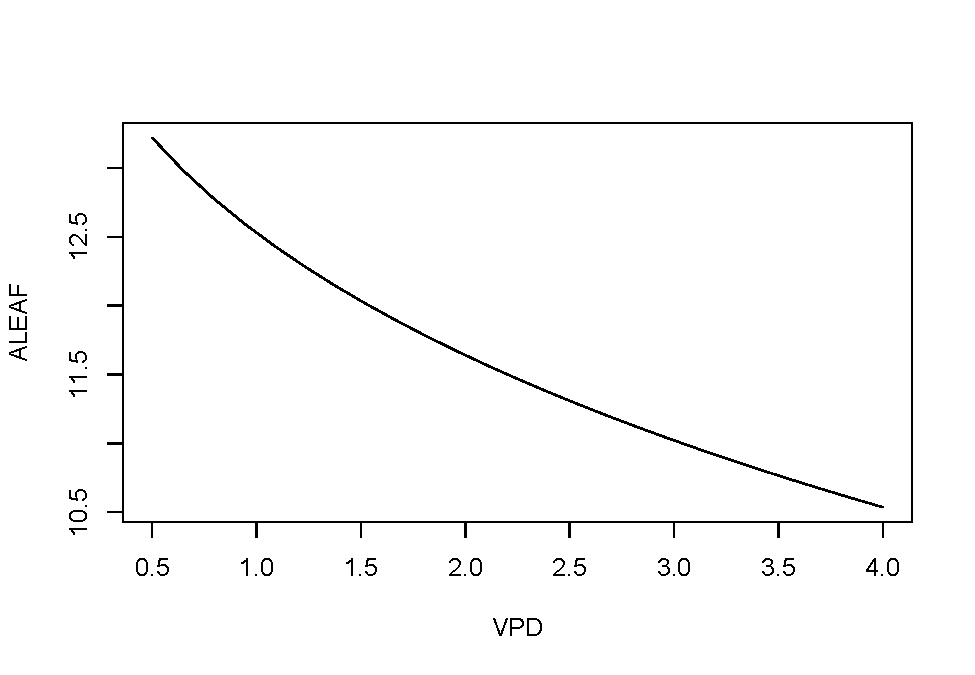
\includegraphics{bookdown_files/figure-latex/vpd-1.pdf}
\caption{\label{fig:vpd}VPD VS. An}
\end{figure}

不同 VPD 下的光合速率见 \ref{fig:vpd}。

\begin{Shaded}
\begin{Highlighting}[]
\CommentTok{# 设定叶肉导度的拟合}
\NormalTok{run1 <-}\StringTok{ }\KeywordTok{Photosyn}\NormalTok{(}\DataTypeTok{PPFD=}\KeywordTok{seq}\NormalTok{(}\DecValTok{50}\NormalTok{,}\DecValTok{1000}\NormalTok{,}\DataTypeTok{length=}\DecValTok{25}\NormalTok{), }
                 \DataTypeTok{gmeso=}\FloatTok{0.15}\NormalTok{, }\DataTypeTok{Vcmax=}\DecValTok{40}\NormalTok{, }\DataTypeTok{Jmax=}\DecValTok{85}\NormalTok{)}
\KeywordTok{with}\NormalTok{(run1, }\KeywordTok{plot}\NormalTok{(PPFD, GS, }\DataTypeTok{type=}\StringTok{'l'}\NormalTok{))}
\end{Highlighting}
\end{Shaded}

\begin{figure}
\centering
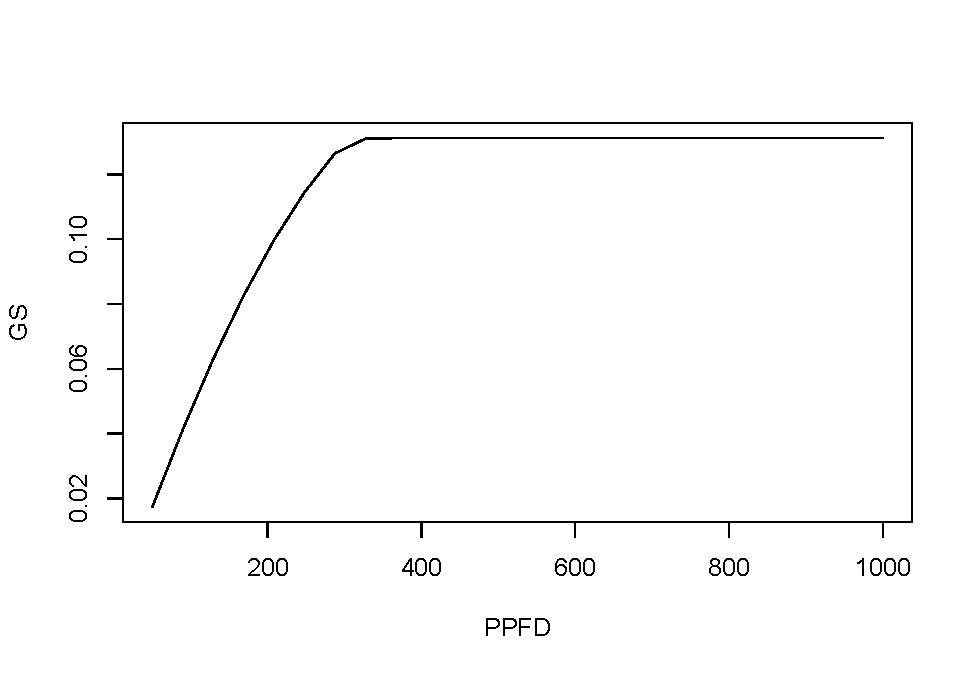
\includegraphics{bookdown_files/figure-latex/ppfd-1.pdf}
\caption{\label{fig:ppfd1}PPFD VS. GS}
\end{figure}

\begin{Shaded}
\begin{Highlighting}[]
\CommentTok{# 运行ACi曲线数据(提供Ci值而不是计算)}
\NormalTok{arun1 <-}\StringTok{ }\KeywordTok{Aci}\NormalTok{(}\DataTypeTok{Ci=}\KeywordTok{seq}\NormalTok{(}\DecValTok{50}\NormalTok{, }\DecValTok{1200}\NormalTok{, }\DataTypeTok{length=}\DecValTok{101}\NormalTok{), }
             \DataTypeTok{Vcmax=}\DecValTok{40}\NormalTok{, }\DataTypeTok{Jmax=}\DecValTok{85}\NormalTok{)}
\NormalTok{arun2 <-}\StringTok{ }\KeywordTok{Aci}\NormalTok{(}\DataTypeTok{Ci=}\KeywordTok{seq}\NormalTok{(}\DecValTok{50}\NormalTok{, }\DecValTok{1200}\NormalTok{, }\DataTypeTok{length=}\DecValTok{101}\NormalTok{), }
             \DataTypeTok{Vcmax=}\DecValTok{30}\NormalTok{, }\DataTypeTok{Jmax=}\DecValTok{70}\NormalTok{)}
\KeywordTok{with}\NormalTok{(arun1, }\KeywordTok{plot}\NormalTok{(Ci, ALEAF, }\DataTypeTok{type=}\StringTok{'l'}\NormalTok{))}
\KeywordTok{with}\NormalTok{(arun2, }\KeywordTok{points}\NormalTok{(Ci, ALEAF, }\DataTypeTok{type=}\StringTok{'l'}\NormalTok{, }\DataTypeTok{lty=}\DecValTok{5}\NormalTok{))}
\end{Highlighting}
\end{Shaded}

\begin{figure}
\centering
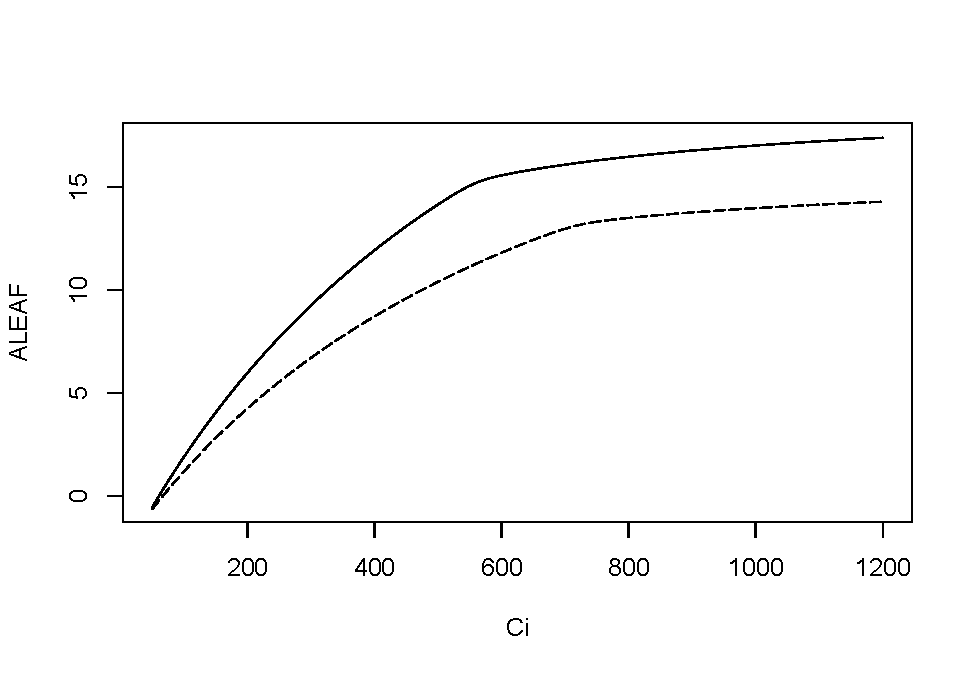
\includegraphics{bookdown_files/figure-latex/ppfd-2.pdf}
\caption{\label{fig:ppfd2}PPFD VS. GS}
\end{figure}

不同 ci 下的光合速率见 \ref{fig:ppfd}。

\begin{Shaded}
\begin{Highlighting}[]
\CommentTok{# 找出CO2需求和供给的交叉点}
\CommentTok{# 设定部分参数}
\NormalTok{gs <-}\StringTok{ }\FloatTok{0.2} \CommentTok{# 对水的气孔导度}
\NormalTok{Ca <-}\StringTok{ }\DecValTok{400} \CommentTok{# 外部CO2}
\NormalTok{gctogw <-}\StringTok{ }\FloatTok{1.57} \CommentTok{# 转换系数}
\NormalTok{gc <-}\StringTok{ }\NormalTok{gs }\OperatorTok{/}\StringTok{ }\NormalTok{gctogw }\CommentTok{# 对 CO2 的气孔导度}
\CommentTok{# 需求曲线}
\NormalTok{p <-}\StringTok{ }\KeywordTok{Aci}\NormalTok{(}\KeywordTok{seq}\NormalTok{(}\DecValTok{60}\NormalTok{,}\DecValTok{500}\NormalTok{,}\DataTypeTok{length=}\DecValTok{101}\NormalTok{), }\DataTypeTok{Ca=}\DecValTok{400}\NormalTok{)}
\CommentTok{# 提供气孔导度及交叉点}
\NormalTok{g <-}\StringTok{ }\KeywordTok{Photosyn}\NormalTok{(}\DataTypeTok{GS=}\NormalTok{gs, }\DataTypeTok{Ca=}\NormalTok{Ca)}
\CommentTok{# 交叉点可视化}
\KeywordTok{par}\NormalTok{(}\DataTypeTok{yaxs=}\StringTok{"i"}\NormalTok{)}
\KeywordTok{with}\NormalTok{(p, }\KeywordTok{plot}\NormalTok{(Ci, ALEAF, }\DataTypeTok{type=}\StringTok{'l'}\NormalTok{, }
             \DataTypeTok{ylim=}\KeywordTok{c}\NormalTok{(}\DecValTok{0}\NormalTok{,}\KeywordTok{max}\NormalTok{(ALEAF))))}
\KeywordTok{with}\NormalTok{(g, }\KeywordTok{points}\NormalTok{(Ci, ALEAF, }\DataTypeTok{pch=}\DecValTok{19}\NormalTok{, }\DataTypeTok{col=}\StringTok{"red"}\NormalTok{))}
\KeywordTok{abline}\NormalTok{(gc }\OperatorTok{*}\StringTok{ }\NormalTok{Ca, }\OperatorTok{-}\NormalTok{gc, }\DataTypeTok{lty=}\DecValTok{5}\NormalTok{)}
\KeywordTok{legend}\NormalTok{(}\StringTok{"topleft"}\NormalTok{, }\KeywordTok{c}\NormalTok{(}\KeywordTok{expression}\NormalTok{(}
  \StringTok{"Demand:"}\OperatorTok{~}\ErrorTok{~}\NormalTok{A}\OperatorTok{==}\KeywordTok{f}\NormalTok{(C[i])),}
   \KeywordTok{expression}\NormalTok{(}\StringTok{"Supply:"}\OperatorTok{~}\ErrorTok{~}\NormalTok{A}\OperatorTok{==}\NormalTok{g[c]}\OperatorTok{*}\NormalTok{(C[a]}\OperatorTok{-}\NormalTok{C[i])),}
              \StringTok{"Operating point"}\NormalTok{),}
   \DataTypeTok{lty=}\KeywordTok{c}\NormalTok{(}\DecValTok{1}\NormalTok{,}\DecValTok{5}\NormalTok{,}\OperatorTok{-}\DecValTok{1}\NormalTok{),}\DataTypeTok{pch=}\KeywordTok{c}\NormalTok{(}\OperatorTok{-}\DecValTok{1}\NormalTok{,}\OperatorTok{-}\DecValTok{1}\NormalTok{,}\DecValTok{19}\NormalTok{),}
   \DataTypeTok{col=}\KeywordTok{c}\NormalTok{(}\StringTok{"black"}\NormalTok{,}\StringTok{"black"}\NormalTok{,}\StringTok{"red"}\NormalTok{),}
   \DataTypeTok{bty=}\StringTok{'n'}\NormalTok{, }\DataTypeTok{cex=}\FloatTok{0.9}\NormalTok{)}
\end{Highlighting}
\end{Shaded}

\begin{figure}
\centering
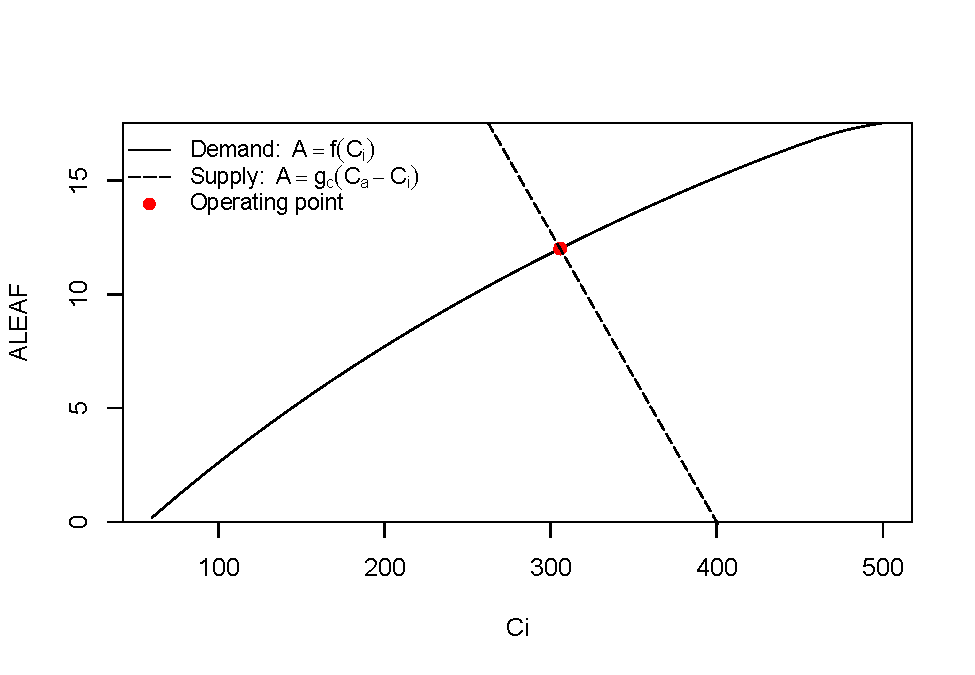
\includegraphics{bookdown_files/figure-latex/supply-1.pdf}
\caption{\label{fig:supply}supply VS. demand}
\end{figure}

需求与供给的作图 \ref{fig:supply}。

\hypertarget{photsyneb}{%
\section{\texorpdfstring{\texttt{PhotosynEB} 函数}{PhotosynEB 函数}}\label{photsyneb}}

使用同 \texttt{Photosyn},只不过使用能量平衡法来计算叶温。
目前版本尚存在bug,不能直接提供 GS 来计算,否则会出现未知错误。

\hypertarget{photosyntuzet}{%
\section{\texorpdfstring{\texttt{PhotosynTuzet} 函数}{PhotosynTuzet 函数}}\label{photosyntuzet}}

同样为光合气孔导度耦合模型,只不过基于 \citet{tuzet2003a} 的气孔导度模型,现将其描述如下:

\begin{equation}
g_{co2} = g_0 + \frac{a A}{C_i - \Gamma} f_{\Psi v}
\label{eq:tuzet}
\end{equation}

其中 g\textsubscript{co2} 为对 CO\textsubscript{2} 的气孔导度, g\textsubscript{0} 是残余导度(residual conductance)(在补偿点时限制 g\textsubscript{CO2} 的值), A 为光合速率,C\textsubscript{i} 为胞间二氧化碳浓度,\(\Gamma\) 为 CO\textsubscript{2} 补偿点,a 是经验系数。

一个根据经验的逻辑方程用于描述气孔对水势的敏感性:

\begin{equation}
f_{\Psi v} = \frac{1 + exp(s_f \Psi_f)}{1 + exp(s_f(\Psi_f - \Psi_v))}
\label{eq:ftuzet}
\end{equation}

\(\Psi_v\) 是指叶片水势,\(\Psi_f\) 是参比势能, 该方程假设在水势接近于 0 时,气孔对叶片水势不敏感,并且气孔随着 \(\Psi_v\) 的下降快速关闭。\(\Psi_f\) 和 \(s_f\) (曲线形状参数) 依赖于不同物种的形态学适应以及生长过程中所处的环境。

\hypertarget{photosyntuzet_para}{%
\subsection{\texorpdfstring{\texttt{PhotosynTuzet} 的参数}{PhotosynTuzet 的参数}}\label{photosyntuzet_para}}

除 \citet{tuzet2003a} 模型中使用的参数外,其他参数都继承了 \texttt{Photosyn} 的参数

\begin{Shaded}
\begin{Highlighting}[]
\KeywordTok{PhotosynTuzet}\NormalTok{(}\DataTypeTok{g1 =} \DecValTok{8}\NormalTok{, }\DataTypeTok{Ca =} \DecValTok{400}\NormalTok{, }\DataTypeTok{psis =} \DecValTok{0}\NormalTok{,}
              \DataTypeTok{kl =} \DecValTok{2}\NormalTok{, }\DataTypeTok{sf =} \DecValTok{3}\NormalTok{, }\DataTypeTok{psif =} \DecValTok{-2}\NormalTok{,}
\NormalTok{...)}
\end{Highlighting}
\end{Shaded}

\begin{itemize}
\tightlist
\item
  g1:斜率参数,要远比 \texttt{fitBB} 中的大。
\item
  Ca:外界大气 CO\textsubscript{2} 浓度
\item
  psis,土壤水势(Mpa)。
\item
  kl:Leaf-specific hydraulic conductance(叶片导水参数 (\(mmol \cdot m^{-2} \cdot s^{-1} \cdot MPa^{-1}\)),叶片蒸腾量、叶片面积及叶片水势计算)。
\item
  sf:曲线形状参数。
\item
  在气孔导度为最大值 50\% 时的叶片水势。
\end{itemize}

\cleardoublepage

\hypertarget{rhtovpd}{%
\chapter{RHtoVPD 函数}\label{rhtovpd}}

该函数为一系列的工具,用于温度、湿度不同单位之间的换算 \citet{Jones1993Plants} :

\begin{Shaded}
\begin{Highlighting}[]
\CommentTok{# RH 转为 VPD  }
\KeywordTok{RHtoVPD}\NormalTok{(RH, TdegC, }\DataTypeTok{Pa =} \DecValTok{101}\NormalTok{) }
 
\CommentTok{# VPD 转为 RH   }
\KeywordTok{VPDtoRH}\NormalTok{(VPD, TdegC, }\DataTypeTok{Pa =} \DecValTok{101}\NormalTok{) }
 
\CommentTok{#  饱和水气压计算 }
\KeywordTok{esat}\NormalTok{(TdegC, }\DataTypeTok{Pa =} \DecValTok{101}\NormalTok{) }
 
\CommentTok{#  露点温度转换为VPD }
\KeywordTok{DewtoVPD}\NormalTok{(Tdew, TdegC, }\DataTypeTok{Pa =} \DecValTok{101}\NormalTok{) }
 
\CommentTok{#  基于叶温的 VPD 转换为基于空气温度的 VPD}
\KeywordTok{VPDleafToAir}\NormalTok{(VPD, Tleaf, Tair, }\DataTypeTok{Pa =} \DecValTok{101}\NormalTok{) }
 
\CommentTok{#  基于空气温度的 VPD 转换为基于叶温的 VPD }
\KeywordTok{VPDairToLeaf}\NormalTok{(VPD, Tair, Tleaf, }\DataTypeTok{Pa =} \DecValTok{101}\NormalTok{) }
 
\CommentTok{#  基于叶温的相对湿度转换为基于空气温度的相对湿度  }
\KeywordTok{RHleafToAir}\NormalTok{(RH, Tleaf, Tair, }\DataTypeTok{Pa =} \DecValTok{101}\NormalTok{) }
 
\CommentTok{#  基于空气温度的相对湿度转换为基于叶温的相对湿度  }
\KeywordTok{RHairToLeaf}\NormalTok{(RH, Tair, Tleaf, }\DataTypeTok{Pa =} \DecValTok{101}\NormalTok{) }
\end{Highlighting}
\end{Shaded}

注意事项及单位:

部分参数的转换需要准确的大气压用于计算,因此,有大气压选项的参数必须填入实际值。

RH:相对湿度 (\%) 。

TdegC:温度 (\textcelsius) (叶片或温度)。

Pa:大气压 (kPa)

VPD:水气压亏缺 (kPa)。

Tdew: 露点温度(\textcelsius) 。

Tleaf:叶温(\textcelsius) 。

Tair:空气温度(\textcelsius) 。

\cleardoublepage

\hypertarget{lrc_fit}{%
\chapter{光响应曲线的拟合}\label{lrc_fit}}

光响应曲线模型有很多,主要分为四大类,直角双曲线,非直角双曲线,指数以及直角双曲线修正模型,我们分别对这四类进行阐述。

\hypertarget{rec_mod}{%
\section{直角双曲线模型}\label{rec_mod}}

\citet{BalyEC1935} 提出了直角双曲线模型,它的表达式为:

\begin{equation}
P_{n}  = \frac{\alpha I\ P_{nmax}}{\alpha I + P_{nmax}}- R_{d}
\label{eq:rec}
\end{equation}

\begin{itemize}
\tightlist
\item
  其中,P\(_{n}\) 为净光合速率;
\item
  I 为光强;
\item
  \(\alpha\) 为光响应曲线在光强为0时的斜率,即光响应曲线的初始斜率,也称之为初始量子效率;
\item
  \(P_{nmax}\) 为最大净光合速率;
\item
  \(R_{d}\):为暗呼吸速率。
\end{itemize}

对 \eqref{eq:rec} 求导可知其导数大于 0,也就是直角双曲线是一个没有极值的渐近线,因此,无法由 \eqref{eq:rec} 求得最大光合速率的饱和光强\footnote{直角双曲线和非直角双曲线模型类似,如果测量时饱和光强之后光合速率不下降,则计算的P\(_{nmax}\)则远大于实测值。}。

因此就需要使用弱光条件下
(\(\leq\) 200 \(\mu mol\cdot m^{-2}\cdot s^{-1}\)) 的数据得到表观量子效率(apparent
quantum efficiency,AQE),利用非线性最小二乘法估算 P\(_{nmax}\) ,然后利用 \citet{YEZiPiao2010} 的式 \eqref{eq:aqe} 求解 \(I_{sat}\),

\begin{equation}
P_{nmax}= AQE \times I_{sat} - R_{d}
\label{eq:aqe}
\end{equation}

但此方法测得的光饱和点远小于实测值,我们采用 0.7P\(_{nmax}\) \citet{ZhangXS2009}、0.9P\(_{nmax}\)
\citet{HuangHY2009}、或其他设定的值来的来估算\(I_{sat}\)。

\hypertarget{rec_fit}{%
\subsection{直角双曲线模型的实现}\label{rec_fit}}

若没有安装 \texttt{minpack.lm}, 则需要首先:

\begin{Shaded}
\begin{Highlighting}[]
\KeywordTok{install.packages}\NormalTok{(}\StringTok{"minpack.lm"}\NormalTok{)}
\end{Highlighting}
\end{Shaded}

具体实现过程如下:

\begin{Shaded}
\begin{Highlighting}[]
\CommentTok{# 调用非线性拟合包minpack.lm,也可以直接使用nls}
\KeywordTok{library}\NormalTok{(minpack.lm)}
\CommentTok{# 读取数据,同fitaci数据格式}
\NormalTok{lrc <-}\StringTok{ }\KeywordTok{read.csv}\NormalTok{(}\StringTok{"./data/lrc.csv"}\NormalTok{)}
\NormalTok{lrc <-}\StringTok{ }\KeywordTok{subset}\NormalTok{(lrc, Obs }\OperatorTok{>}\StringTok{ }\DecValTok{0}\NormalTok{)}

\CommentTok{# 光响应曲线没有太多参数,}
\CommentTok{# 直接调出相应的光强和光合速率}
\CommentTok{# 方便后面调用}
\NormalTok{lrc_Q <-}\StringTok{ }\NormalTok{lrc}\OperatorTok{$}\NormalTok{PARi}
\NormalTok{lrc_A <-}\StringTok{ }\NormalTok{lrc}\OperatorTok{$}\NormalTok{Photo }

\CommentTok{# 采用非线性拟合进行数据的拟合}
\NormalTok{lrcnls <-}\StringTok{ }\KeywordTok{nlsLM}\NormalTok{(lrc_A }\OperatorTok{~}\StringTok{ }\NormalTok{(alpha }\OperatorTok{*}\StringTok{ }\NormalTok{lrc_Q }\OperatorTok{*}\StringTok{ }\NormalTok{Am) }\OperatorTok{*}\StringTok{ }
\StringTok{                }\NormalTok{(}\DecValTok{1}\OperatorTok{/}\NormalTok{(alpha }\OperatorTok{*}\StringTok{ }\NormalTok{lrc_Q }\OperatorTok{+}\StringTok{ }\NormalTok{Am)) }\OperatorTok{-}\StringTok{ }\NormalTok{Rd,  }
              \DataTypeTok{start=}\KeywordTok{list}\NormalTok{(}\DataTypeTok{Am=}\NormalTok{(}\KeywordTok{max}\NormalTok{(lrc_A)}\OperatorTok{-}\KeywordTok{min}\NormalTok{(lrc_A)),}
              \DataTypeTok{alpha=}\FloatTok{0.05}\NormalTok{,}\DataTypeTok{Rd=}\OperatorTok{-}\KeywordTok{min}\NormalTok{(lrc_A))}
\NormalTok{)}
\NormalTok{fitlrc_rec <-}\StringTok{ }\KeywordTok{summary}\NormalTok{(lrcnls)}

\CommentTok{# 补偿点时净光合速率为0,}
\CommentTok{# 据此利用uniroot求解方程的根}
\NormalTok{Ic <-}\StringTok{ }\ControlFlowTok{function}\NormalTok{(Ic)\{(fitlrc_rec}\OperatorTok{$}\NormalTok{coef[}\DecValTok{2}\NormalTok{,}\DecValTok{1}\NormalTok{] }\OperatorTok{*}\StringTok{ }\NormalTok{Ic }\OperatorTok{*}
\StringTok{    }\NormalTok{fitlrc_rec}\OperatorTok{$}\NormalTok{coef[}\DecValTok{1}\NormalTok{,}\DecValTok{1}\NormalTok{]) }\OperatorTok{*}\StringTok{ }\NormalTok{(}\DecValTok{1}\OperatorTok{/}\NormalTok{(fitlrc_rec}\OperatorTok{$}\NormalTok{coef[}\DecValTok{2}\NormalTok{,}\DecValTok{1}\NormalTok{] }\OperatorTok{*}\StringTok{ }
\StringTok{    }\NormalTok{Ic }\OperatorTok{+}\StringTok{ }\NormalTok{fitlrc_rec}\OperatorTok{$}\NormalTok{coef[}\DecValTok{1}\NormalTok{,}\DecValTok{1}\NormalTok{])) }\OperatorTok{-}\StringTok{ }\NormalTok{fitlrc_rec}\OperatorTok{$}\NormalTok{coef[}\DecValTok{3}\NormalTok{,}\DecValTok{1}\NormalTok{] }
\NormalTok{\}}

\KeywordTok{uniroot}\NormalTok{(Ic, }\KeywordTok{c}\NormalTok{(}\DecValTok{0}\NormalTok{,}\DecValTok{50}\NormalTok{))}\OperatorTok{$}\NormalTok{root}
\end{Highlighting}
\end{Shaded}

\begin{verbatim}
## [1] 3.650053
\end{verbatim}

\begin{Shaded}
\begin{Highlighting}[]
\CommentTok{# 根据饱和点定义,0.75最大光合速率为饱和点,}
\CommentTok{# 也可以是其他比例}
\CommentTok{# 据此利用uniroot求解方程的根}

\NormalTok{Isat <-}\StringTok{ }\ControlFlowTok{function}\NormalTok{(Isat)\{(fitlrc_rec}\OperatorTok{$}\NormalTok{coef[}\DecValTok{2}\NormalTok{,}\DecValTok{1}\NormalTok{] }\OperatorTok{*}\StringTok{ }
\StringTok{        }\NormalTok{Isat }\OperatorTok{*}\StringTok{ }\NormalTok{fitlrc_rec}\OperatorTok{$}\NormalTok{coef[}\DecValTok{1}\NormalTok{,}\DecValTok{1}\NormalTok{]) }\OperatorTok{*}\StringTok{ }
\StringTok{    }\NormalTok{(}\DecValTok{1}\OperatorTok{/}\NormalTok{(fitlrc_rec}\OperatorTok{$}\NormalTok{coef[}\DecValTok{2}\NormalTok{,}\DecValTok{1}\NormalTok{] }\OperatorTok{*}\StringTok{ }\NormalTok{Isat }\OperatorTok{+}\StringTok{ }
\StringTok{          }\NormalTok{fitlrc_rec}\OperatorTok{$}\NormalTok{coef[}\DecValTok{1}\NormalTok{,}\DecValTok{1}\NormalTok{])) }\OperatorTok{-}\StringTok{ }\NormalTok{fitlrc_rec}\OperatorTok{$}\NormalTok{coef[}\DecValTok{3}\NormalTok{,}\DecValTok{1}\NormalTok{] }\OperatorTok{-}
\StringTok{    }\FloatTok{0.75} \OperatorTok{*}\StringTok{ }\NormalTok{fitlrc_rec}\OperatorTok{$}\NormalTok{coef[}\DecValTok{1}\NormalTok{,}\DecValTok{1}\NormalTok{]}
\NormalTok{\}}
\CommentTok{# 求值区间根据具体实验确定}

\KeywordTok{uniroot}\NormalTok{(Isat, }\KeywordTok{c}\NormalTok{(}\DecValTok{0}\NormalTok{,}\DecValTok{2500}\NormalTok{))}\OperatorTok{$}\NormalTok{root}
\end{Highlighting}
\end{Shaded}

\begin{verbatim}
## [1] 700.0946
\end{verbatim}

\begin{Shaded}
\begin{Highlighting}[]
\CommentTok{# 使用ggplot2进行作图并拟合曲线}
\KeywordTok{library}\NormalTok{(ggplot2)}
\end{Highlighting}
\end{Shaded}

\begin{verbatim}
## Registered S3 methods overwritten by 'ggplot2':
##   method         from 
##   [.quosures     rlang
##   c.quosures     rlang
##   print.quosures rlang
\end{verbatim}

\begin{Shaded}
\begin{Highlighting}[]
\NormalTok{light <-}\StringTok{ }\KeywordTok{data.frame}\NormalTok{(}\DataTypeTok{lrc_Q =}\NormalTok{ lrc}\OperatorTok{$}\NormalTok{PARi, }\DataTypeTok{lrc_A =}\NormalTok{ lrc}\OperatorTok{$}\NormalTok{Photo)}

\NormalTok{p <-}\StringTok{ }\KeywordTok{ggplot}\NormalTok{(light, }\KeywordTok{aes}\NormalTok{(}\DataTypeTok{x =}\NormalTok{ lrc_Q, }\DataTypeTok{y =}\NormalTok{ lrc_A))}

\NormalTok{p1 <-}\StringTok{ }\NormalTok{p }\OperatorTok{+}\StringTok{ }\KeywordTok{geom_point}\NormalTok{(}\DataTypeTok{shape =} \DecValTok{16}\NormalTok{, }\DataTypeTok{size =} \DecValTok{3}\NormalTok{, }\DataTypeTok{color =} \StringTok{"green"}\NormalTok{) }\OperatorTok{+}\StringTok{ }
\StringTok{  }\KeywordTok{geom_smooth}\NormalTok{(}\DataTypeTok{method=}\StringTok{"nls"}\NormalTok{, }\DataTypeTok{formula =}\NormalTok{ y }\OperatorTok{~}\StringTok{ }\NormalTok{(alpha }\OperatorTok{*}\StringTok{ }\NormalTok{x }\OperatorTok{*}\StringTok{ }\NormalTok{Am) }\OperatorTok{*}\StringTok{ }
\StringTok{  }\NormalTok{(}\DecValTok{1}\OperatorTok{/}\NormalTok{(alpha }\OperatorTok{*}\StringTok{ }\NormalTok{x }\OperatorTok{+}\StringTok{ }\NormalTok{Am)) }\OperatorTok{-}\StringTok{ }\NormalTok{Rd, }\DataTypeTok{se =} \OtherTok{FALSE}\NormalTok{,}
  \DataTypeTok{method.args =} 
  \KeywordTok{list}\NormalTok{(}\DataTypeTok{start =} \KeywordTok{c}\NormalTok{(}\DataTypeTok{Am=}\NormalTok{(}\KeywordTok{max}\NormalTok{(lrc_A)}\OperatorTok{-}\KeywordTok{min}\NormalTok{(lrc_A)),}
  \DataTypeTok{alpha=}\FloatTok{0.05}\NormalTok{,}\DataTypeTok{Rd=}\OperatorTok{-}\KeywordTok{min}\NormalTok{(lrc_A)), }
  \KeywordTok{aes}\NormalTok{(}\DataTypeTok{x =}\NormalTok{lrc_Q, }\DataTypeTok{y =}\NormalTok{ lrc_A, }\DataTypeTok{color=}\StringTok{'blue'}\NormalTok{, }\DataTypeTok{size =} \FloatTok{1.2}\NormalTok{))}
\NormalTok{  ) }\OperatorTok{+}
\StringTok{  }\KeywordTok{labs}\NormalTok{(}\DataTypeTok{y=}\KeywordTok{expression}\NormalTok{(}\KeywordTok{paste}\NormalTok{(}\StringTok{"photosynthetic rate  "}\NormalTok{, }
       \StringTok{"("}\NormalTok{, mu, mol}\OperatorTok\NormalTok{m}\OperatorTok{^-}\DecValTok{2}\OperatorTok\NormalTok{s}\OperatorTok{^-}\DecValTok{1}\NormalTok{, }\StringTok{")"}\NormalTok{)), }
       \DataTypeTok{x=}\KeywordTok{expression}\NormalTok{(}\KeywordTok{paste}\NormalTok{(}\StringTok{"PAR "}\NormalTok{, }
       \StringTok{"("}\NormalTok{, mu, mol}\OperatorTok\NormalTok{m}\OperatorTok{^-}\DecValTok{2}\OperatorTok\NormalTok{s}\OperatorTok{^-}\DecValTok{1}\NormalTok{, }\StringTok{")"}\NormalTok{))}
\NormalTok{       )}


\CommentTok{# 自定义坐标轴}
\NormalTok{p1 }\OperatorTok{+}\StringTok{ }\KeywordTok{scale_x_continuous}\NormalTok{(}\DataTypeTok{breaks =} \KeywordTok{seq}\NormalTok{(}\DecValTok{0}\NormalTok{, }\DecValTok{2100}\NormalTok{, }\DataTypeTok{by =} \DecValTok{200}\NormalTok{)) }\OperatorTok{+}\StringTok{  }
\StringTok{  }\KeywordTok{scale_y_continuous}\NormalTok{(}\DataTypeTok{breaks=} \KeywordTok{round}\NormalTok{(light}\OperatorTok{$}\NormalTok{lrc_A)) }\OperatorTok{+}
\StringTok{  }\KeywordTok{theme}\NormalTok{(}\DataTypeTok{axis.text.x  =} \KeywordTok{element_text}\NormalTok{(}
    \DataTypeTok{size =} \DecValTok{10}\NormalTok{, }\DataTypeTok{angle=}\DecValTok{30}\NormalTok{, }\DataTypeTok{vjust=}\FloatTok{0.5}\NormalTok{), }
    \DataTypeTok{axis.text.y =} \KeywordTok{element_text}\NormalTok{(}\DataTypeTok{size =} \DecValTok{10}\NormalTok{),}
    \DataTypeTok{axis.title.x =} \KeywordTok{element_text}\NormalTok{(}\DataTypeTok{size =} \DecValTok{12}\NormalTok{, }\DataTypeTok{face =} \StringTok{'bold'}\NormalTok{),}
    \DataTypeTok{axis.title.y =} \KeywordTok{element_text}\NormalTok{(}\DataTypeTok{size =} \DecValTok{12}\NormalTok{, }\DataTypeTok{face =} \StringTok{'bold'}\NormalTok{)}
\NormalTok{  )}
\end{Highlighting}
\end{Shaded}

\begin{figure}
\centering
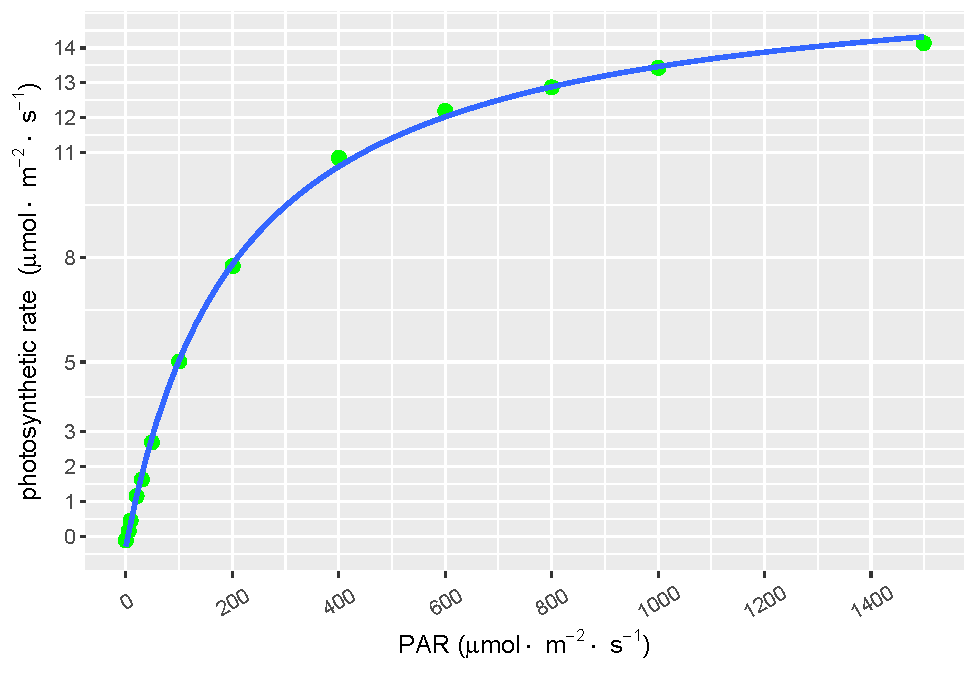
\includegraphics{bookdown_files/figure-latex/recr-1.pdf}
\caption{\label{fig:recr}直角双曲线模型拟合}
\end{figure}

代码目的见注释,其实现过程主要分三步:

\begin{itemize}
\tightlist
\item
  数据的导入,这与之前相同,具体格式方法参考前文 \ref{fitaci}。
\item
  光响应曲线的拟合,使用到了非线性模型 nlsLM,也可以使用 nls,具体实现方法请查看参考文档。
\item
  求饱和点和补偿点,补偿点的计算根据其定义,净光合速率为 0,求解模型在一定区间的根来计算,而饱和点则较为麻烦,若使用式 \eqref{eq:aqe}
  计算,那么饱和点远远低于我们实际需求的,因此,我们使用了 0.75P\(_{nmax}\) 来计算,求得目标区间的根。当然也可以采用其他比例来作为饱和点光合速率。
\end{itemize}

\begin{table}[t]

\caption{\label{tab:rectable}直角双曲线计算参数}
\centering
\begin{tabular}{lrrrr}
\toprule
  & Estimate & Std. Error & t value & Pr(>|t|)\\
\midrule
Am & 16.6721752 & 0.1522849 & 109.480151 & 0.0000000\\
alpha & 0.0783312 & 0.0026774 & 29.256870 & 0.0000000\\
Rd & 0.2810926 & 0.0789338 & 3.561117 & 0.0051716\\
\bottomrule
\end{tabular}
\end{table}

最终的数据拟结果如图 \ref{fig:recr} 所示,拟合的参数及结果见表 \ref{tab:rectable}。

\cleardoublepage

\hypertarget{nonrec_mod}{%
\section{非直角双曲线模型}\label{nonrec_mod}}

\citet{Thornley1976} 提出了非直角双曲线模型,它的表达式为:

\begin{equation}
P_{n} = \frac{\alpha I + P_{nmax} \sqrt{(\alpha I + P_{nmax})^{2} - 4  \theta \alpha I P_{nmax}}}{2 \theta} - R_{d}
\label{eq:nrec}
\end{equation}

其中,\(\theta\) 为表示曲线弯曲程度的曲角参数,取值为\(0\leq \theta \leq 1\)。其他参数意义同式 \eqref{eq:rec}。同样如同直角双曲线模型,式仍然没有极值,无法求得 \(I_{sat}\),可以仍然参考直角双曲线模型的方式进行计算。

\hypertarget{nonrec_mode_exam}{%
\subsection{非直角双曲线模型的实现}\label{nonrec_mode_exam}}

\begin{Shaded}
\begin{Highlighting}[]
\KeywordTok{library}\NormalTok{(minpack.lm)}

\CommentTok{# 读取数据,同fitaci数据格式}
\NormalTok{lrc <-}\StringTok{ }\KeywordTok{read.csv}\NormalTok{(}\StringTok{"./data/lrc.csv"}\NormalTok{)}
\NormalTok{lrc <-}\StringTok{ }\KeywordTok{subset}\NormalTok{(lrc, Obs }\OperatorTok{>}\StringTok{ }\DecValTok{0}\NormalTok{)}

\CommentTok{# 光响应曲线没有太多参数,}
\CommentTok{# 直接调出相应的光强和光合速率}
\CommentTok{# 方便后面调用}
\NormalTok{lrc_Q <-}\StringTok{ }\NormalTok{lrc}\OperatorTok{$}\NormalTok{PARi}
\NormalTok{lrc_A <-}\StringTok{ }\NormalTok{lrc}\OperatorTok{$}\NormalTok{Photo }

\CommentTok{# 非直角双曲线模型的拟合}
\NormalTok{lrcnls <-}\StringTok{ }\KeywordTok{nlsLM}\NormalTok{(lrc_A }\OperatorTok{~}\StringTok{ }
\StringTok{                }\NormalTok{(}\DecValTok{1}\OperatorTok{/}\NormalTok{(}\DecValTok{2}\OperatorTok{*}\NormalTok{theta))}\OperatorTok{*}
\StringTok{                }\NormalTok{(alpha}\OperatorTok{*}\NormalTok{lrc_Q}\OperatorTok{+}\NormalTok{Am}\OperatorTok{-}\KeywordTok{sqrt}\NormalTok{((alpha}\OperatorTok{*}\NormalTok{lrc_Q}\OperatorTok{+}\NormalTok{Am)}\OperatorTok{^}\DecValTok{2} \OperatorTok{-}\StringTok{ }
\StringTok{                }\DecValTok{4}\OperatorTok{*}\NormalTok{alpha}\OperatorTok{*}\NormalTok{theta}\OperatorTok{*}\NormalTok{Am}\OperatorTok{*}\NormalTok{lrc_Q))}\OperatorTok{-}\StringTok{ }\NormalTok{Rd,}
                \DataTypeTok{start=}\KeywordTok{list}\NormalTok{(}\DataTypeTok{Am=}\NormalTok{(}\KeywordTok{max}\NormalTok{(lrc_A)}\OperatorTok{-}\KeywordTok{min}\NormalTok{(lrc_A)),}
                \DataTypeTok{alpha=}\FloatTok{0.05}\NormalTok{,}\DataTypeTok{Rd=}\OperatorTok{-}\KeywordTok{min}\NormalTok{(lrc_A),}\DataTypeTok{theta=}\DecValTok{1}\NormalTok{)) }

\NormalTok{fitlrc_nrec <-}\StringTok{ }\KeywordTok{summary}\NormalTok{(lrcnls)}

\CommentTok{# 光补偿点}
\NormalTok{Ic <-}\StringTok{ }\ControlFlowTok{function}\NormalTok{(Ic)\{}
\NormalTok{  (}\DecValTok{1}\OperatorTok{/}\NormalTok{(}\DecValTok{2} \OperatorTok{*}\StringTok{ }\NormalTok{fitlrc_nrec}\OperatorTok{$}\NormalTok{coef[}\DecValTok{4}\NormalTok{,}\DecValTok{1}\NormalTok{])) }\OperatorTok{*}\StringTok{ }
\StringTok{    }\NormalTok{(fitlrc_nrec}\OperatorTok{$}\NormalTok{coef[}\DecValTok{2}\NormalTok{,}\DecValTok{1}\NormalTok{] }\OperatorTok{*}\StringTok{ }\NormalTok{Ic }\OperatorTok{+}\StringTok{ }\NormalTok{fitlrc_nrec}\OperatorTok{$}\NormalTok{coef[}\DecValTok{1}\NormalTok{,}\DecValTok{1}\NormalTok{] }\OperatorTok{-}\StringTok{ }
\StringTok{    }\KeywordTok{sqrt}\NormalTok{((fitlrc_nrec}\OperatorTok{$}\NormalTok{coef[}\DecValTok{2}\NormalTok{,}\DecValTok{1}\NormalTok{] }\OperatorTok{*}\StringTok{ }\NormalTok{Ic }\OperatorTok{+}\StringTok{ }\NormalTok{fitlrc_nrec}\OperatorTok{$}\NormalTok{coef[}\DecValTok{1}\NormalTok{,}\DecValTok{1}\NormalTok{]}
\NormalTok{    )}\OperatorTok{^}\DecValTok{2} \OperatorTok{-}\StringTok{  }\DecValTok{4} \OperatorTok{*}\StringTok{ }\NormalTok{fitlrc_nrec}\OperatorTok{$}\NormalTok{coef[}\DecValTok{2}\NormalTok{,}\DecValTok{1}\NormalTok{] }\OperatorTok{*}\StringTok{ }
\StringTok{    }\NormalTok{fitlrc_nrec}\OperatorTok{$}\NormalTok{coef[}\DecValTok{4}\NormalTok{,}\DecValTok{1}\NormalTok{] }\OperatorTok{*}\StringTok{ }\NormalTok{fitlrc_nrec}\OperatorTok{$}\NormalTok{coef[}\DecValTok{1}\NormalTok{,}\DecValTok{1}\NormalTok{] }\OperatorTok{*}\StringTok{ }\NormalTok{Ic)) }\OperatorTok{-}
\StringTok{    }\NormalTok{fitlrc_nrec}\OperatorTok{$}\NormalTok{coef[}\DecValTok{3}\NormalTok{,}\DecValTok{1}\NormalTok{]}
\NormalTok{\}}

\KeywordTok{uniroot}\NormalTok{(Ic, }\KeywordTok{c}\NormalTok{(}\DecValTok{0}\NormalTok{,}\DecValTok{50}\NormalTok{))}\OperatorTok{$}\NormalTok{root  }
\end{Highlighting}
\end{Shaded}

\begin{verbatim}
## [1] 2.234292
\end{verbatim}

\begin{Shaded}
\begin{Highlighting}[]
\CommentTok{# 光饱和点}
\NormalTok{Isat <-}\StringTok{ }\ControlFlowTok{function}\NormalTok{(Isat)\{}
\NormalTok{  (}\DecValTok{1}\OperatorTok{/}\NormalTok{(}\DecValTok{2} \OperatorTok{*}\StringTok{ }\NormalTok{fitlrc_nrec}\OperatorTok{$}\NormalTok{coef[}\DecValTok{4}\NormalTok{,}\DecValTok{1}\NormalTok{])) }\OperatorTok{*}\StringTok{ }\NormalTok{(fitlrc_nrec}\OperatorTok{$}\NormalTok{coef[}\DecValTok{2}\NormalTok{,}\DecValTok{1}\NormalTok{] }\OperatorTok{*}\StringTok{ }
\StringTok{  }\NormalTok{Isat }\OperatorTok{+}\StringTok{ }\NormalTok{fitlrc_nrec}\OperatorTok{$}\NormalTok{coef[}\DecValTok{1}\NormalTok{,}\DecValTok{1}\NormalTok{] }\OperatorTok{-}\StringTok{ }\KeywordTok{sqrt}\NormalTok{(}
\NormalTok{  (fitlrc_nrec}\OperatorTok{$}\NormalTok{coef[}\DecValTok{2}\NormalTok{,}\DecValTok{1}\NormalTok{] }\OperatorTok{*}\StringTok{ }\NormalTok{Isat }\OperatorTok{+}\NormalTok{fitlrc_nrec}\OperatorTok{$}\NormalTok{coef[}\DecValTok{1}\NormalTok{,}\DecValTok{1}\NormalTok{])}\OperatorTok{^}\DecValTok{2} \OperatorTok{-}\StringTok{ }
\StringTok{  }\DecValTok{4}\OperatorTok{*}\NormalTok{fitlrc_nrec}\OperatorTok{$}\NormalTok{coef[}\DecValTok{2}\NormalTok{,}\DecValTok{1}\NormalTok{] }\OperatorTok{*}\StringTok{ }\NormalTok{fitlrc_nrec}\OperatorTok{$}\NormalTok{coef[}\DecValTok{4}\NormalTok{,}\DecValTok{1}\NormalTok{] }\OperatorTok{*}\StringTok{ }
\StringTok{  }\NormalTok{fitlrc_nrec}\OperatorTok{$}\NormalTok{coef[}\DecValTok{1}\NormalTok{,}\DecValTok{1}\NormalTok{] }\OperatorTok{*}\StringTok{ }\NormalTok{Isat)) }\OperatorTok{-}\StringTok{ }
\StringTok{  }\NormalTok{fitlrc_nrec}\OperatorTok{$}\NormalTok{coef[}\DecValTok{3}\NormalTok{,}\DecValTok{1}\NormalTok{] }\OperatorTok{-}\StringTok{ }\NormalTok{(}\FloatTok{0.9}\OperatorTok{*}\NormalTok{fitlrc_nrec}\OperatorTok{$}\NormalTok{coef[}\DecValTok{1}\NormalTok{,}\DecValTok{1}\NormalTok{])\}}

\KeywordTok{uniroot}\NormalTok{(Isat, }\KeywordTok{c}\NormalTok{(}\DecValTok{0}\NormalTok{,}\DecValTok{2000}\NormalTok{))}\OperatorTok{$}\NormalTok{root}
\end{Highlighting}
\end{Shaded}

\begin{verbatim}
## [1] 1596.286
\end{verbatim}

\begin{Shaded}
\begin{Highlighting}[]
\CommentTok{# 使用ggplot2进行作图并拟合曲线}
\KeywordTok{library}\NormalTok{(ggplot2)}
\NormalTok{light <-}\StringTok{ }\KeywordTok{data.frame}\NormalTok{(}\DataTypeTok{lrc_Q =}\NormalTok{ lrc}\OperatorTok{$}\NormalTok{PARi, }\DataTypeTok{lrc_A =}\NormalTok{ lrc}\OperatorTok{$}\NormalTok{Photo)}

\NormalTok{p <-}\StringTok{ }\KeywordTok{ggplot}\NormalTok{(light, }\KeywordTok{aes}\NormalTok{(}\DataTypeTok{x =}\NormalTok{ lrc_Q, }\DataTypeTok{y =}\NormalTok{ lrc_A))}

\NormalTok{p1 <-}\StringTok{ }\NormalTok{p }\OperatorTok{+}\StringTok{ }\KeywordTok{geom_point}\NormalTok{(}\DataTypeTok{shape =} \DecValTok{16}\NormalTok{, }\DataTypeTok{size =} \DecValTok{3}\NormalTok{, }\DataTypeTok{color =} \StringTok{"green"}\NormalTok{) }\OperatorTok{+}\StringTok{ }
\StringTok{  }\KeywordTok{geom_smooth}\NormalTok{(}\DataTypeTok{method=}\StringTok{"nls"}\NormalTok{, }\DataTypeTok{formula =}\NormalTok{ y }\OperatorTok{~}\StringTok{ }
\StringTok{  }\NormalTok{(}\DecValTok{1}\OperatorTok{/}\NormalTok{(}\DecValTok{2}\OperatorTok{*}\NormalTok{theta))}\OperatorTok{*}\NormalTok{(alpha}\OperatorTok{*}\NormalTok{x}\OperatorTok{+}\NormalTok{Am}\OperatorTok{-}\KeywordTok{sqrt}\NormalTok{((alpha}\OperatorTok{*}\NormalTok{x}\OperatorTok{+}\NormalTok{Am)}\OperatorTok{^}\DecValTok{2} \OperatorTok{-}\StringTok{ }
\StringTok{   }\DecValTok{4}\OperatorTok{*}\NormalTok{alpha}\OperatorTok{*}\NormalTok{theta}\OperatorTok{*}\NormalTok{Am}\OperatorTok{*}\NormalTok{x))}\OperatorTok{-}\StringTok{ }\NormalTok{Rd, }\DataTypeTok{se =} \OtherTok{FALSE}\NormalTok{,}
   \DataTypeTok{method.args =} \KeywordTok{list}\NormalTok{(}\DataTypeTok{start =} \KeywordTok{c}\NormalTok{(}\DataTypeTok{Am=}\NormalTok{(}\KeywordTok{max}\NormalTok{(lrc_A)}\OperatorTok{-}\KeywordTok{min}\NormalTok{(lrc_A)), }
   \DataTypeTok{alpha=}\FloatTok{0.05}\NormalTok{, }\DataTypeTok{Rd=}\OperatorTok{-}\KeywordTok{min}\NormalTok{(lrc_A), }\DataTypeTok{theta=}\DecValTok{1}\NormalTok{), }
    \KeywordTok{aes}\NormalTok{(}\DataTypeTok{x =}\NormalTok{lrc_Q, }\DataTypeTok{y =}\NormalTok{ lrc_A, }\DataTypeTok{color=}\StringTok{'blue'}\NormalTok{, }\DataTypeTok{size =} \FloatTok{1.2}\NormalTok{))}
\NormalTok{) }\OperatorTok{+}
\StringTok{  }\KeywordTok{labs}\NormalTok{(}\DataTypeTok{y=}\KeywordTok{expression}\NormalTok{(}\KeywordTok{paste}\NormalTok{(}\StringTok{"photosynthetic rate  "}\NormalTok{, }
          \StringTok{"("}\NormalTok{, mu, mol}\OperatorTok\NormalTok{m}\OperatorTok{^-}\DecValTok{2}\OperatorTok\NormalTok{s}\OperatorTok{^-}\DecValTok{1}\NormalTok{, }\StringTok{")"}\NormalTok{)), }
       \DataTypeTok{x=}\KeywordTok{expression}\NormalTok{(}\KeywordTok{paste}\NormalTok{(}\StringTok{"PAR "}\NormalTok{, }
           \StringTok{"("}\NormalTok{, mu, mol}\OperatorTok\NormalTok{m}\OperatorTok{^-}\DecValTok{2}\OperatorTok\NormalTok{s}\OperatorTok{^-}\DecValTok{1}\NormalTok{, }\StringTok{")"}\NormalTok{)))}

\CommentTok{# 自定义坐标轴}
\NormalTok{p1 }\OperatorTok{+}\StringTok{ }\KeywordTok{scale_x_continuous}\NormalTok{(}\DataTypeTok{breaks =} \KeywordTok{seq}\NormalTok{(}\DecValTok{0}\NormalTok{, }\DecValTok{2100}\NormalTok{, }\DataTypeTok{by =} \DecValTok{200}\NormalTok{)) }\OperatorTok{+}\StringTok{  }
\StringTok{  }\KeywordTok{scale_y_continuous}\NormalTok{(}\DataTypeTok{breaks=} \KeywordTok{round}\NormalTok{(light}\OperatorTok{$}\NormalTok{lrc_A)) }\OperatorTok{+}
\StringTok{   }\KeywordTok{theme}\NormalTok{(}\DataTypeTok{axis.text.x  =} \KeywordTok{element_text}\NormalTok{(}
    \DataTypeTok{size =} \DecValTok{10}\NormalTok{, }\DataTypeTok{angle=}\DecValTok{30}\NormalTok{, }\DataTypeTok{vjust=}\FloatTok{0.5}\NormalTok{), }
    \DataTypeTok{axis.text.y =} \KeywordTok{element_text}\NormalTok{(}\DataTypeTok{size =} \DecValTok{10}\NormalTok{),}
    \DataTypeTok{axis.title.x =} \KeywordTok{element_text}\NormalTok{(}\DataTypeTok{size =} \DecValTok{12}\NormalTok{, }\DataTypeTok{face =} \StringTok{'bold'}\NormalTok{),}
    \DataTypeTok{axis.title.y =} \KeywordTok{element_text}\NormalTok{(}\DataTypeTok{size =} \DecValTok{12}\NormalTok{, }\DataTypeTok{face =} \StringTok{'bold'}\NormalTok{)}
\NormalTok{  )}
\end{Highlighting}
\end{Shaded}

\begin{figure}
\centering
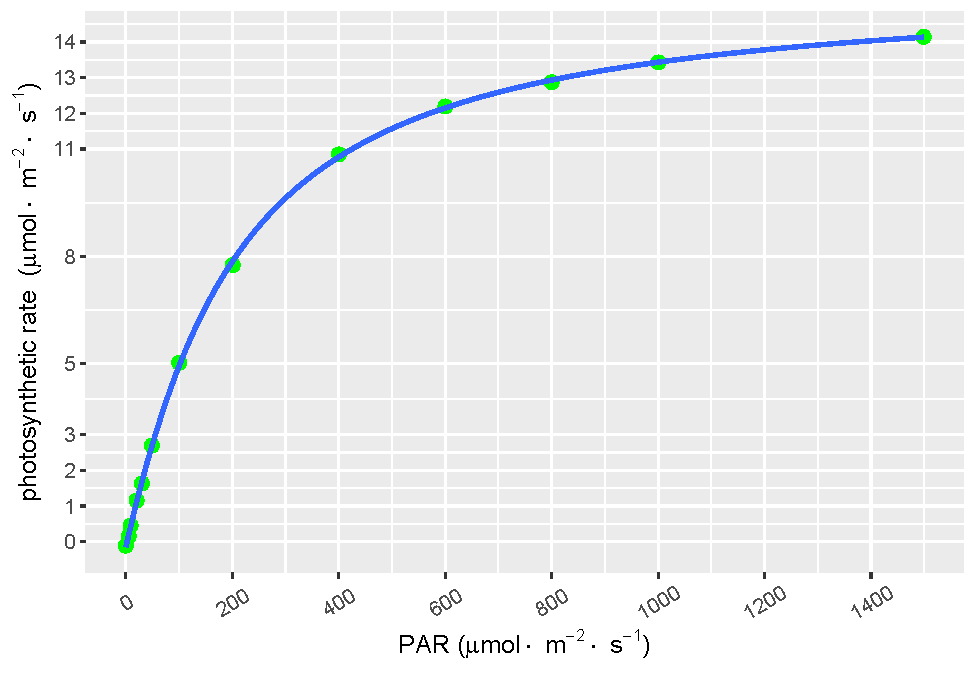
\includegraphics{bookdown_files/figure-latex/nrecr-1.pdf}
\caption{\label{fig:nrecr}非直角双曲线模型拟合}
\end{figure}

\begin{table}[t]

\caption{\label{tab:nrectable}非直角双曲线计算参数}
\centering
\begin{tabular}{lrrrr}
\toprule
  & Estimate & Std. Error & t value & Pr(>|t|)\\
\midrule
Am & 15.8017296 & 0.1513064 & 104.435285 & 0.0000000\\
alpha & 0.0658067 & 0.0020216 & 32.551422 & 0.0000000\\
Rd & 0.1461717 & 0.0420800 & 3.473659 & 0.0070082\\
theta & 0.3700908 & 0.0493403 & 7.500783 & 0.0000369\\
\bottomrule
\end{tabular}
\end{table}

最终的数据拟结果如图 \ref{fig:nrecr} 所示,拟合的参数及结果见表 \ref{tab:nrectable}。单纯从作图来看,本例数据使用非直角双曲线与散点图重合程度更高。

\cleardoublepage

\hypertarget{lrc_exp}{%
\section{指数模型}\label{lrc_exp}}

光合指数模型较多,我们此处使用的指数函数的模型 \citet{Prado1997Photosynthetic},其表达式为:

\begin{equation}
P_{n} = P_{nmax}[1 - e^{-b(I-I_{C})}]
\label{eq:exp}
\end{equation}

其中,\(I_{c}\) 为光补偿点,\(e\) 为自然对数的底,b为常数,其他参数意义同 \eqref{eq:exp}。同样,该方程仍然是没有极值的函数,但我们可以直接求得光补偿点。

\hypertarget{lrc_exp_exam}{%
\subsection{指数模型的实现}\label{lrc_exp_exam}}

\begin{Shaded}
\begin{Highlighting}[]
\KeywordTok{library}\NormalTok{(minpack.lm)}

\CommentTok{# 读取数据,同fitaci数据格式}
\NormalTok{lrc <-}\StringTok{ }\KeywordTok{read.csv}\NormalTok{(}\StringTok{"./data/lrc.csv"}\NormalTok{)}
\NormalTok{lrc <-}\StringTok{ }\KeywordTok{subset}\NormalTok{(lrc, Obs }\OperatorTok{>}\StringTok{ }\DecValTok{0}\NormalTok{)}

\CommentTok{# 光响应曲线没有太多参数,}
\CommentTok{# 直接调出相应的光强和光合速率}
\CommentTok{# 方便后面调用}
\NormalTok{lrc_Q <-}\StringTok{ }\NormalTok{lrc}\OperatorTok{$}\NormalTok{PARi}
\NormalTok{lrc_A <-}\StringTok{ }\NormalTok{lrc}\OperatorTok{$}\NormalTok{Photo }

\CommentTok{# 模型的拟合}
\NormalTok{lrcnls <-}\StringTok{ }\KeywordTok{nlsLM}\NormalTok{(lrc_A }\OperatorTok{~}\StringTok{ }\NormalTok{Am}\OperatorTok{*}\NormalTok{(}\DecValTok{1}\OperatorTok{-}\KeywordTok{exp}\NormalTok{((}\OperatorTok{-}\NormalTok{b)}\OperatorTok{*}\NormalTok{(lrc_Q}\OperatorTok{-}\NormalTok{Ic))),}
                \DataTypeTok{start=}\KeywordTok{list}\NormalTok{(}\DataTypeTok{Am=}\NormalTok{(}\KeywordTok{max}\NormalTok{(lrc_A)}\OperatorTok{-}\KeywordTok{min}\NormalTok{(lrc_A)),}
                           \DataTypeTok{Ic=}\DecValTok{5}\NormalTok{, }\DataTypeTok{b=}\DecValTok{1}\NormalTok{)}
\NormalTok{                )}
\NormalTok{fitlrc_exp <-}\StringTok{ }\KeywordTok{summary}\NormalTok{(lrcnls)}

\CommentTok{# 光饱和点}
\NormalTok{Isat <-}\StringTok{ }\ControlFlowTok{function}\NormalTok{(Isat)\{fitlrc_exp}\OperatorTok{$}\NormalTok{coef[}\DecValTok{1}\NormalTok{,}\DecValTok{1}\NormalTok{]}\OperatorTok{*}
\StringTok{    }\NormalTok{(}\DecValTok{1}\OperatorTok{-}\KeywordTok{exp}\NormalTok{((}\OperatorTok{-}\NormalTok{fitlrc_exp}\OperatorTok{$}\NormalTok{coef[}\DecValTok{3}\NormalTok{,}\DecValTok{1}\NormalTok{])}\OperatorTok{*}\NormalTok{(Isat}\OperatorTok{-}
\StringTok{    }\NormalTok{fitlrc_exp}\OperatorTok{$}\NormalTok{coef[}\DecValTok{2}\NormalTok{,}\DecValTok{1}\NormalTok{])))}\OperatorTok{-}\FloatTok{0.9}\OperatorTok{*}\NormalTok{fitlrc_exp}\OperatorTok{$}\NormalTok{coef[}\DecValTok{1}\NormalTok{,}\DecValTok{1}\NormalTok{]\}}

\KeywordTok{uniroot}\NormalTok{(Isat, }\KeywordTok{c}\NormalTok{(}\DecValTok{0}\NormalTok{,}\DecValTok{2000}\NormalTok{))}\OperatorTok{$}\NormalTok{root}
\end{Highlighting}
\end{Shaded}

\begin{verbatim}
## [1] 558.6038
\end{verbatim}

\begin{Shaded}
\begin{Highlighting}[]
\CommentTok{## 拟合图形}
\KeywordTok{library}\NormalTok{(ggplot2)}
\NormalTok{light <-}\StringTok{ }\KeywordTok{data.frame}\NormalTok{(}\DataTypeTok{lrc_Q =}\NormalTok{ lrc}\OperatorTok{$}\NormalTok{PARi, }\DataTypeTok{lrc_A =}\NormalTok{ lrc}\OperatorTok{$}\NormalTok{Photo)}

\NormalTok{p <-}\StringTok{ }\KeywordTok{ggplot}\NormalTok{(light, }\KeywordTok{aes}\NormalTok{(}\DataTypeTok{x =}\NormalTok{ lrc_Q, }\DataTypeTok{y =}\NormalTok{ lrc_A))}

\NormalTok{p1 <-}\StringTok{ }\NormalTok{p }\OperatorTok{+}\StringTok{ }
\StringTok{  }\KeywordTok{geom_point}\NormalTok{(}\DataTypeTok{shape =} \DecValTok{16}\NormalTok{, }\DataTypeTok{size =} \DecValTok{3}\NormalTok{, }\DataTypeTok{color =} \StringTok{"green"}\NormalTok{) }\OperatorTok{+}\StringTok{ }
\StringTok{  }\KeywordTok{geom_smooth}\NormalTok{(}\DataTypeTok{method=}\StringTok{"nls"}\NormalTok{, }\DataTypeTok{formula =} 
\NormalTok{    y }\OperatorTok{~}\StringTok{ }\NormalTok{Am}\OperatorTok{*}\NormalTok{(}\DecValTok{1}\OperatorTok{-}\KeywordTok{exp}\NormalTok{((}\OperatorTok{-}\NormalTok{b)}\OperatorTok{*}\NormalTok{(x }\OperatorTok{-}\NormalTok{Ic))), }
    \DataTypeTok{se =} \OtherTok{FALSE}\NormalTok{, }\DataTypeTok{method.args =} \KeywordTok{list}\NormalTok{(}
    \DataTypeTok{start =} \KeywordTok{c}\NormalTok{(}\DataTypeTok{Am=}\NormalTok{(}\KeywordTok{max}\NormalTok{(lrc_A)}\OperatorTok{-}\KeywordTok{min}\NormalTok{(lrc_A)),}
    \DataTypeTok{Ic=}\DecValTok{5}\NormalTok{, }\DataTypeTok{b=}\FloatTok{0.002}\NormalTok{), }\KeywordTok{aes}\NormalTok{(}\DataTypeTok{x =}\NormalTok{lrc_Q, }\DataTypeTok{y =}\NormalTok{ lrc_A, }
    \DataTypeTok{color=}\StringTok{'blue'}\NormalTok{, }\DataTypeTok{size =} \FloatTok{1.2}\NormalTok{))}
\NormalTok{  ) }\OperatorTok{+}
\StringTok{  }\KeywordTok{labs}\NormalTok{(}\DataTypeTok{y=}\KeywordTok{expression}\NormalTok{(}\KeywordTok{paste}\NormalTok{(}\StringTok{"photosynthetic rate  "}\NormalTok{, }
          \StringTok{"("}\NormalTok{, mu, mol}\OperatorTok\NormalTok{m}\OperatorTok{^-}\DecValTok{2}\OperatorTok\NormalTok{s}\OperatorTok{^-}\DecValTok{1}\NormalTok{, }\StringTok{")"}\NormalTok{)), }
       \DataTypeTok{x=}\KeywordTok{expression}\NormalTok{(}\KeywordTok{paste}\NormalTok{(}\StringTok{"PAR "}\NormalTok{, }
           \StringTok{"("}\NormalTok{, mu, mol}\OperatorTok\NormalTok{m}\OperatorTok{^-}\DecValTok{2}\OperatorTok\NormalTok{s}\OperatorTok{^-}\DecValTok{1}\NormalTok{, }\StringTok{")"}\NormalTok{)))}


\CommentTok{# 自定义坐标轴}
\NormalTok{p1 }\OperatorTok{+}\StringTok{ }\KeywordTok{scale_x_continuous}\NormalTok{(}\DataTypeTok{breaks =} \KeywordTok{seq}\NormalTok{(}\DecValTok{0}\NormalTok{, }\DecValTok{2100}\NormalTok{, }\DataTypeTok{by =} \DecValTok{200}\NormalTok{)) }\OperatorTok{+}\StringTok{  }
\StringTok{  }\KeywordTok{scale_y_continuous}\NormalTok{(}\DataTypeTok{breaks=} \KeywordTok{round}\NormalTok{(light}\OperatorTok{$}\NormalTok{lrc_A)) }\OperatorTok{+}
\StringTok{   }\KeywordTok{theme}\NormalTok{(}\DataTypeTok{axis.text.x  =} \KeywordTok{element_text}\NormalTok{(}
    \DataTypeTok{size =} \DecValTok{10}\NormalTok{, }\DataTypeTok{angle=}\DecValTok{30}\NormalTok{, }\DataTypeTok{vjust=}\FloatTok{0.5}\NormalTok{), }
    \DataTypeTok{axis.text.y =} \KeywordTok{element_text}\NormalTok{(}\DataTypeTok{size =} \DecValTok{10}\NormalTok{),}
    \DataTypeTok{axis.title.x =} \KeywordTok{element_text}\NormalTok{(}\DataTypeTok{size =} \DecValTok{12}\NormalTok{, }\DataTypeTok{face =} \StringTok{'bold'}\NormalTok{),}
    \DataTypeTok{axis.title.y =} \KeywordTok{element_text}\NormalTok{(}\DataTypeTok{size =} \DecValTok{12}\NormalTok{, }\DataTypeTok{face =} \StringTok{'bold'}\NormalTok{)}
\NormalTok{  )}
\end{Highlighting}
\end{Shaded}

\begin{figure}
\centering
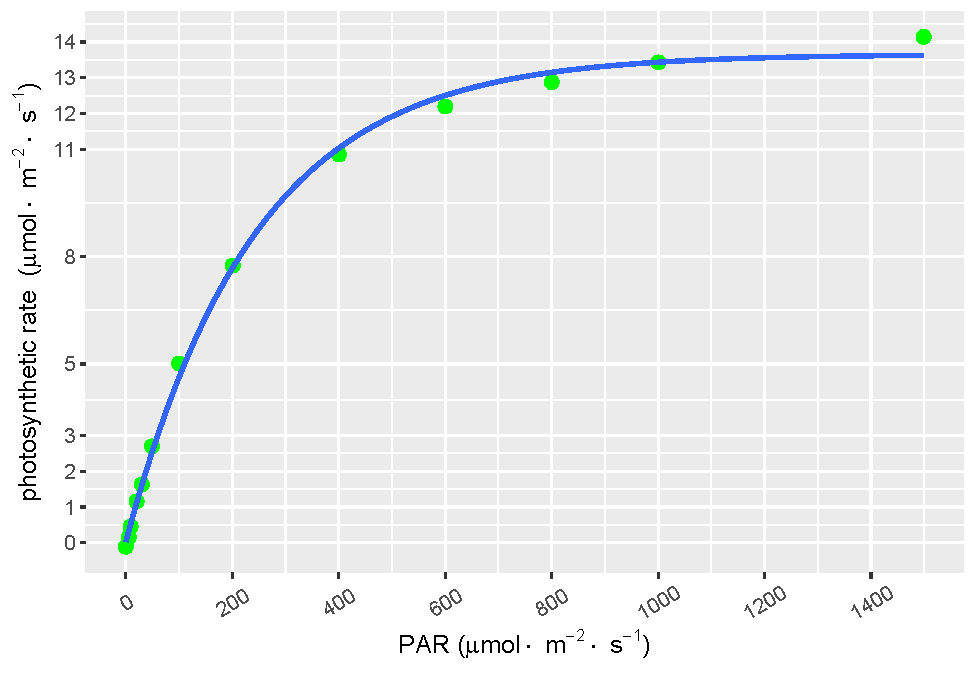
\includegraphics{bookdown_files/figure-latex/nexpr-1.pdf}
\caption{\label{fig:nexpr}指数模型拟合}
\end{figure}

\begin{table}[t]

\caption{\label{tab:nexptable}指数模型计算参数}
\centering
\begin{tabular}{lrrrr}
\toprule
  & Estimate & Std. Error & t value & Pr(>|t|)\\
\midrule
Am & 13.6547568 & 0.1723363 & 79.233185 & 0.0000000\\
Ic & -0.5133438 & 2.3370250 & -0.219657 & 0.8305573\\
b & 0.0041183 & 0.0002012 & 20.467032 & 0.0000000\\
\bottomrule
\end{tabular}
\end{table}

最终的数据拟结果如图 \ref{fig:nexpr} 所示,拟合的参数及结果见表 \ref{tab:nexptable}。

\cleardoublepage

\hypertarget{rev_rec}{%
\section{直角双曲线的修正模型}\label{rev_rec}}

\citet{YEZiPiao2010} 直角双曲线修正模型的表达式如式 \eqref{eq:mrec} 所示:

\begin{equation}
P_{n} = \alpha \frac{1-\beta I}{1+\gamma I} I - R_{d}
\label{eq:mrec}
\end{equation}

其中,\(\beta\) 和 \(\gamma\) 为系数,\(\beta\)光抑制项,\(\gamma\)光饱和项,单位为
\(m^{2}\cdot s\cdot\mu mol^{-1}\),其他参数与上文相同,因为该式 \eqref{eq:mrec}
存在极值,因此,必然存在饱和光强和最大净光合速率,分别用式 \eqref{eq:isat} 和式 \eqref{eq:ic} 求得。

\begin{equation}
I_{sat} = \frac{\sqrt{\frac{(\beta+\gamma)}{\beta}-1}}{\gamma}
\label{eq:isat}
\end{equation}

\begin{equation}
P_{nmax} = \alpha\left(\frac{\sqrt{\beta+\gamma}-\sqrt{\beta}}{\gamma}\right)^{2}-R_{d}
\label{eq:ic}
\end{equation}

该模型的优点为拟合结果中光饱和点和最大净光合速率均接近实测值,还可以拟合饱和光强之后光合速率随光强下降段的曲线。

\hypertarget{rev_rec_exam}{%
\subsection{直角双曲线修正模型的实现}\label{rev_rec_exam}}

\begin{Shaded}
\begin{Highlighting}[]
\KeywordTok{library}\NormalTok{(minpack.lm)}

\CommentTok{# 读取数据,同fitaci数据格式}
\NormalTok{lrc <-}\StringTok{ }\KeywordTok{read.csv}\NormalTok{(}\StringTok{"./data/lrc.csv"}\NormalTok{)}
\NormalTok{lrc <-}\StringTok{ }\KeywordTok{subset}\NormalTok{(lrc, Obs }\OperatorTok{>}\StringTok{ }\DecValTok{0}\NormalTok{)}

\CommentTok{# 光响应曲线没有太多参数,}
\CommentTok{# 直接调出相应的光强和光合速率}
\CommentTok{# 方便后面调用}
\NormalTok{lrc_Q <-}\StringTok{ }\NormalTok{lrc}\OperatorTok{$}\NormalTok{PARi}
\NormalTok{lrc_A <-}\StringTok{ }\NormalTok{lrc}\OperatorTok{$}\NormalTok{Photo }

\CommentTok{# 模型的拟合}
\NormalTok{lrcnls <-}\StringTok{ }\KeywordTok{nlsLM}\NormalTok{(lrc_A }\OperatorTok{~}\StringTok{ }\NormalTok{alpha }\OperatorTok{*}\StringTok{ }\NormalTok{((}\DecValTok{1} \OperatorTok{-}\StringTok{ }
\StringTok{              }\NormalTok{beta}\OperatorTok{*}\NormalTok{lrc_Q)}\OperatorTok{/}\NormalTok{(}\DecValTok{1} \OperatorTok{+}\StringTok{ }\NormalTok{gamma }\OperatorTok{*}\StringTok{ }\NormalTok{lrc_Q)) }\OperatorTok{*}\StringTok{ }\NormalTok{lrc_Q }\OperatorTok{-}\StringTok{ }\NormalTok{Rd,}
                \DataTypeTok{start=}\KeywordTok{list}\NormalTok{(}\DataTypeTok{alpha =} \FloatTok{0.07}\NormalTok{, }\DataTypeTok{beta =} \FloatTok{0.00005}\NormalTok{,}
                           \DataTypeTok{gamma=}\FloatTok{0.004}\NormalTok{, }\DataTypeTok{Rd =} \FloatTok{0.2}\NormalTok{)}
\NormalTok{                )}
\NormalTok{fitlrc_mrec <-}\StringTok{ }\KeywordTok{summary}\NormalTok{(lrcnls)}

\CommentTok{# 饱和点计算}
\NormalTok{Isat <-}\StringTok{  }\KeywordTok{sqrt}\NormalTok{((fitlrc_mrec}\OperatorTok{$}\NormalTok{coef[}\DecValTok{2}\NormalTok{,}\DecValTok{1}\NormalTok{] }\OperatorTok{+}\StringTok{ }\NormalTok{fitlrc_mrec}\OperatorTok{$}\NormalTok{coef[}\DecValTok{3}\NormalTok{,}\DecValTok{1}\NormalTok{])}\OperatorTok{/}
\StringTok{              }\NormalTok{fitlrc_mrec}\OperatorTok{$}\NormalTok{coef[}\DecValTok{2}\NormalTok{,}\DecValTok{1}\NormalTok{]}\OperatorTok{-}\DecValTok{1}\NormalTok{)}\OperatorTok{/}\NormalTok{fitlrc_mrec}\OperatorTok{$}\NormalTok{coef[}\DecValTok{3}\NormalTok{,}\DecValTok{1}\NormalTok{]}
\CommentTok{# 补偿点计算}
\NormalTok{Ic <-}\StringTok{ }\NormalTok{(fitlrc_mrec}\OperatorTok{$}\NormalTok{coef[}\DecValTok{1}\NormalTok{,}\DecValTok{1}\NormalTok{] }\OperatorTok{-}\StringTok{ }\NormalTok{fitlrc_mrec}\OperatorTok{$}\NormalTok{coef[}\DecValTok{4}\NormalTok{,}\DecValTok{1}\NormalTok{])}\OperatorTok{/}
\StringTok{  }\NormalTok{(fitlrc_mrec}\OperatorTok{$}\NormalTok{coef[}\DecValTok{3}\NormalTok{,}\DecValTok{1}\NormalTok{]}\OperatorTok{*}\NormalTok{fitlrc_mrec}\OperatorTok{$}\NormalTok{coef[}\DecValTok{4}\NormalTok{,}\DecValTok{1}\NormalTok{]}\OperatorTok{+}
\StringTok{   }\NormalTok{fitlrc_mrec}\OperatorTok{$}\NormalTok{coef[}\DecValTok{1}\NormalTok{,}\DecValTok{1}\NormalTok{]}\OperatorTok{*}\NormalTok{fitlrc_mrec}\OperatorTok{$}\NormalTok{coef[}\DecValTok{2}\NormalTok{,}\DecValTok{1}\NormalTok{])}

\CommentTok{## 拟合图形}
\KeywordTok{library}\NormalTok{(ggplot2)}
\NormalTok{light <-}\StringTok{ }\KeywordTok{data.frame}\NormalTok{(}\DataTypeTok{lrc_Q =}\NormalTok{ lrc}\OperatorTok{$}\NormalTok{PARi, }\DataTypeTok{lrc_A =}\NormalTok{ lrc}\OperatorTok{$}\NormalTok{Photo)}

\NormalTok{p <-}\StringTok{ }\KeywordTok{ggplot}\NormalTok{(light, }\KeywordTok{aes}\NormalTok{(}\DataTypeTok{x =}\NormalTok{ lrc_Q, }\DataTypeTok{y =}\NormalTok{ lrc_A))}

\NormalTok{p1 <-}\StringTok{ }\NormalTok{p }\OperatorTok{+}\StringTok{ }
\StringTok{  }\KeywordTok{geom_point}\NormalTok{(}\DataTypeTok{shape =} \DecValTok{16}\NormalTok{, }\DataTypeTok{size =} \DecValTok{3}\NormalTok{, }\DataTypeTok{color =} \StringTok{"green"}\NormalTok{) }\OperatorTok{+}\StringTok{ }
\StringTok{  }\KeywordTok{geom_smooth}\NormalTok{(}\DataTypeTok{method=}\StringTok{"nls"}\NormalTok{, }\DataTypeTok{formula =} 
\NormalTok{   y }\OperatorTok{~}\StringTok{ }\NormalTok{alpha }\OperatorTok{*}\StringTok{ }\NormalTok{((}\DecValTok{1} \OperatorTok{-}\StringTok{ }
\StringTok{              }\NormalTok{beta}\OperatorTok{*}\NormalTok{x)}\OperatorTok{/}\NormalTok{(}\DecValTok{1} \OperatorTok{+}\StringTok{ }\NormalTok{gamma }\OperatorTok{*}\StringTok{ }\NormalTok{x)) }\OperatorTok{*}\StringTok{ }\NormalTok{x }\OperatorTok{-}\StringTok{ }\NormalTok{Rd, }
    \DataTypeTok{se =} \OtherTok{FALSE}\NormalTok{, }\DataTypeTok{method.args =} \KeywordTok{list}\NormalTok{(}
    \DataTypeTok{start =} \KeywordTok{c}\NormalTok{(}\DataTypeTok{alpha =} \FloatTok{0.07}\NormalTok{, }\DataTypeTok{beta =} \FloatTok{0.00005}\NormalTok{,}
              \DataTypeTok{gamma=}\FloatTok{0.004}\NormalTok{, }\DataTypeTok{Rd =} \FloatTok{0.2}\NormalTok{), }
    \KeywordTok{aes}\NormalTok{(}\DataTypeTok{x =}\NormalTok{lrc_Q, }\DataTypeTok{y =}\NormalTok{ lrc_A, }
    \DataTypeTok{color=}\StringTok{'blue'}\NormalTok{, }\DataTypeTok{size =} \FloatTok{1.2}\NormalTok{))}
\NormalTok{  ) }\OperatorTok{+}
\StringTok{  }\KeywordTok{labs}\NormalTok{(}\DataTypeTok{y=}\KeywordTok{expression}\NormalTok{(}\KeywordTok{paste}\NormalTok{(}\StringTok{"photosynthetic rate  "}\NormalTok{, }
          \StringTok{"("}\NormalTok{, mu, mol}\OperatorTok\NormalTok{m}\OperatorTok{^-}\DecValTok{2}\OperatorTok\NormalTok{s}\OperatorTok{^-}\DecValTok{1}\NormalTok{, }\StringTok{")"}\NormalTok{)), }
       \DataTypeTok{x=}\KeywordTok{expression}\NormalTok{(}\KeywordTok{paste}\NormalTok{(}\StringTok{"PAR "}\NormalTok{, }
           \StringTok{"("}\NormalTok{, mu, mol}\OperatorTok\NormalTok{m}\OperatorTok{^-}\DecValTok{2}\OperatorTok\NormalTok{s}\OperatorTok{^-}\DecValTok{1}\NormalTok{, }\StringTok{")"}\NormalTok{)))}


\CommentTok{# 自定义坐标轴}
\NormalTok{p1 }\OperatorTok{+}\StringTok{ }\KeywordTok{scale_x_continuous}\NormalTok{(}\DataTypeTok{breaks =} \KeywordTok{seq}\NormalTok{(}\DecValTok{0}\NormalTok{, }\DecValTok{2100}\NormalTok{, }\DataTypeTok{by =} \DecValTok{200}\NormalTok{)) }\OperatorTok{+}\StringTok{  }
\StringTok{  }\KeywordTok{scale_y_continuous}\NormalTok{(}\DataTypeTok{breaks=} \KeywordTok{round}\NormalTok{(light}\OperatorTok{$}\NormalTok{lrc_A)) }\OperatorTok{+}
\StringTok{   }\KeywordTok{theme}\NormalTok{(}\DataTypeTok{axis.text.x  =} \KeywordTok{element_text}\NormalTok{(}
    \DataTypeTok{size =} \DecValTok{10}\NormalTok{, }\DataTypeTok{angle=}\DecValTok{30}\NormalTok{, }\DataTypeTok{vjust=}\FloatTok{0.5}\NormalTok{), }
    \DataTypeTok{axis.text.y =} \KeywordTok{element_text}\NormalTok{(}\DataTypeTok{size =} \DecValTok{10}\NormalTok{),}
    \DataTypeTok{axis.title.x =} \KeywordTok{element_text}\NormalTok{(}\DataTypeTok{size =} \DecValTok{12}\NormalTok{, }\DataTypeTok{face =} \StringTok{'bold'}\NormalTok{),}
    \DataTypeTok{axis.title.y =} \KeywordTok{element_text}\NormalTok{(}\DataTypeTok{size =} \DecValTok{12}\NormalTok{, }\DataTypeTok{face =} \StringTok{'bold'}\NormalTok{)}
\NormalTok{  )}
\end{Highlighting}
\end{Shaded}

\begin{figure}
\centering
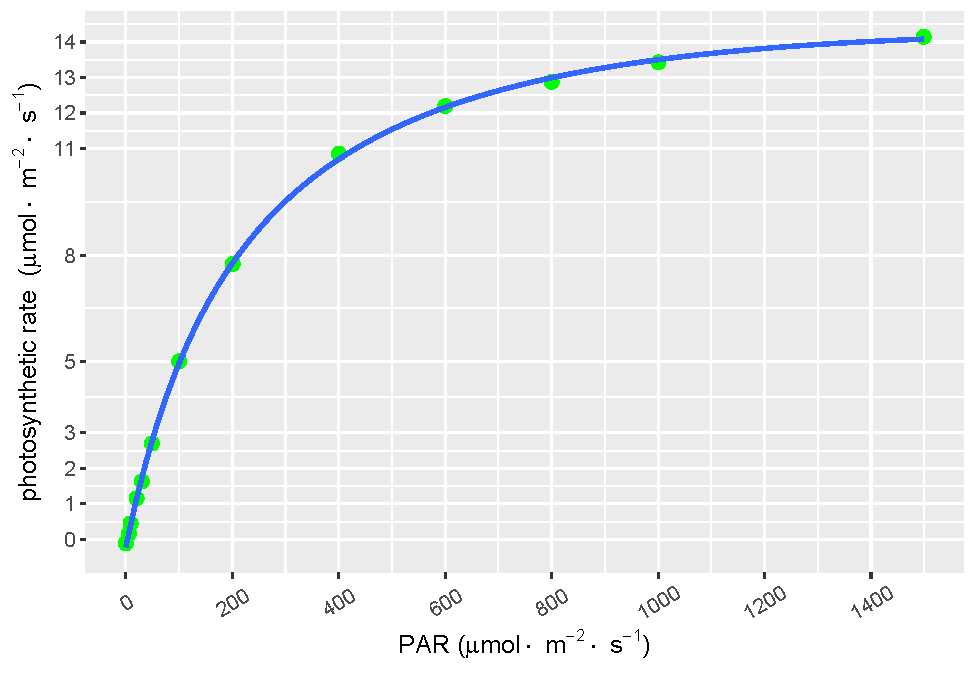
\includegraphics{bookdown_files/figure-latex/mrecr-1.pdf}
\caption{\label{fig:mrecr}直角双曲线修正模型拟合}
\end{figure}

\begin{table}[t]

\caption{\label{tab:mrectable}直角双曲线修正模型计算参数}
\centering
\begin{tabular}{lrrrr}
\toprule
  & Estimate & Std. Error & t value & Pr(>|t|)\\
\midrule
alpha & 0.0730858 & 0.0021209 & 34.460183 & 0.0000000\\
beta & 0.0000501 & 0.0000133 & 3.776115 & 0.0043751\\
gamma & 0.0040622 & 0.0001955 & 20.773916 & 0.0000000\\
Rd & 0.2156186 & 0.0543505 & 3.967190 & 0.0032685\\
\bottomrule
\end{tabular}
\end{table}

尽管修正模型可以方便的计算饱和点和补偿点,但如同 \citet{Lobo2013Fitting} 所指出,双曲线模型对其结果的计算常有超出生态学意义范围的值\footnote{例如本例的数据结果},因此对模型的选择不能一概而论,需根据实际情况而选择。

\cleardoublepage

\hypertarget{start_con}{%
\chapter{关于非线性拟合的初始值}\label{start_con}}

在解释初始值之前我们首先需要了解一个数学上的概念------迭代,

\begin{quote}
``迭代法''也称``辗转法''是一种不断用变量的旧值递推新值的过程。
\end{quote}

用通俗但不是特别严谨的说法可解释为:每次执行这种算法是,程序都会从原值(也就是我抄的上面迭代法定义的旧值)推出一个新值。

之所以先介绍这个迭代,原因很简单,非线性拟合就是通过迭代的方法,需要对每一个变量\textbf{最初的估计值进行不断的迭代,得到一个向一个点收缩或汇聚的值,这个估计值必须在实际值的一定范围内,程序通过不断调整这个值来改善拟合结果}。这就解释了上面的问题,初始值是让程序开始运行的前提,不然没法迭代,必须设定。我下面的内容将以 LI-6800 的光响应曲线的测试数据,使用非直角双曲线模型进行拟合来讲解具体的 R 中的一些实现方法,我们首先导入数据,然后再利用这些数据逐个举例不同的确定初始值的方式。

\begin{Shaded}
\begin{Highlighting}[]
\NormalTok{nls <-}\StringTok{ }\KeywordTok{read.csv}\NormalTok{(}\StringTok{"data/nlstest.csv"}\NormalTok{)}


\CommentTok{# 光响应曲线比较简单,我们将需要的数据直接提取,方便后面操作}
\NormalTok{lrc_Q <-}\StringTok{ }\NormalTok{nls}\OperatorTok{$}\NormalTok{Qin}
\NormalTok{lrc_A <-}\StringTok{ }\NormalTok{nls}\OperatorTok{$}\NormalTok{A}
\end{Highlighting}
\end{Shaded}

\hypertarget{nlslm}{%
\section{nlsLM 解决方案}\label{nlslm}}

nlsLM 来自于 \citet{Elzhov2016minpack} 的 \texttt{minpack.lm},利用 C 语言的 MINPACK 库,修改了 Levenberg-Marquardt 算法,在实际操作中,很多时候并不准确的输入初始值,他也能得出比较好的拟合结果。但结果未必完美,出现下面让人烦恼的报错:

\begin{quote}
singular gradient matrix at initial parameter estimates
\end{quote}

的概率会大大降低,而且尽管结果不如意,我们也可以利用他的结果缩小初始值的范围,继续尝试其他初始值。

例如下面的例子中,非直角双曲线的 Rd 的初始值我们可以利用暗呼吸的实测值大致估计,同理最大光合速率也是如此,剩下的分别为非直角双曲线曲率,我们暂定为 1,alpha 也暂定为 0.1,使用 \texttt{nlsLM} 进行拟合,结果如下:

\begin{Shaded}
\begin{Highlighting}[]
\KeywordTok{library}\NormalTok{(minpack.lm)}

\NormalTok{lrcnls_lm <-}\StringTok{ }\KeywordTok{nlsLM}\NormalTok{(lrc_A }\OperatorTok{~}\StringTok{ }\NormalTok{(}\DecValTok{1}\OperatorTok{/}\NormalTok{(}\DecValTok{2}\OperatorTok{*}\NormalTok{theta))}\OperatorTok{*}
\StringTok{        }\NormalTok{(alpha}\OperatorTok{*}\NormalTok{lrc_Q}\OperatorTok{+}\NormalTok{Am}\OperatorTok{-}\KeywordTok{sqrt}\NormalTok{((alpha}\OperatorTok{*}\NormalTok{lrc_Q}\OperatorTok{+}\NormalTok{Am)}\OperatorTok{^}\DecValTok{2} \OperatorTok{-}\StringTok{ }
\StringTok{        }\DecValTok{4}\OperatorTok{*}\NormalTok{alpha}\OperatorTok{*}\NormalTok{theta}\OperatorTok{*}\NormalTok{Am}\OperatorTok{*}\NormalTok{lrc_Q))}\OperatorTok{-}\StringTok{ }
\StringTok{        }\NormalTok{Rd, }\DataTypeTok{start=}\KeywordTok{list}\NormalTok{(}\DataTypeTok{Am=}\NormalTok{(}\KeywordTok{max}\NormalTok{(lrc_A)}\OperatorTok{-}\KeywordTok{min}\NormalTok{(lrc_A)),}
        \DataTypeTok{alpha=}\FloatTok{0.1}\NormalTok{,}\DataTypeTok{Rd=}\OperatorTok{-}\KeywordTok{min}\NormalTok{(lrc_A),}\DataTypeTok{theta=}\FloatTok{0.8}\NormalTok{)) }
\end{Highlighting}
\end{Shaded}

结果没有报错,看上去没有问题,那我们观察一下具体的拟合结果:

\begin{Shaded}
\begin{Highlighting}[]
\KeywordTok{summary}\NormalTok{(lrcnls_lm)}
\end{Highlighting}
\end{Shaded}

\begin{verbatim}
## 
## Formula: lrc_A ~ (1/(2 * theta)) * (alpha * lrc_Q + Am - sqrt((alpha * 
##     lrc_Q + Am)^2 - 4 * alpha * theta * Am * lrc_Q)) - Rd
## 
## Parameters:
##        Estimate Std. Error t value Pr(>|t|)    
## Am    12.307570   0.406739  30.259 2.30e-10 ***
## alpha  0.045706   0.003423  13.352 3.09e-07 ***
## Rd     0.656638   0.132646   4.950 0.000791 ***
## theta  0.707522   0.079738   8.873 9.59e-06 ***
## ---
## Signif. codes:  0 '***' 0.001 '**' 0.01 '*' 0.05 '.' 0.1 ' ' 1
## 
## Residual standard error: 0.1852 on 9 degrees of freedom
## 
## Number of iterations to convergence: 8 
## Achieved convergence tolerance: 1.49e-08
\end{verbatim}

结果看上去还可以\footnote{有些时候结果并不理想,该方法并不是万无一失}。

\hypertarget{plot_comp}{%
\section{作图比对法}\label{plot_comp}}

模型很多参数可以用已有数据去估计,我们可以只来分析难以判断的参数,流程如下:

\begin{itemize}
\tightlist
\item
  Rd、Am等我们可以利用测量值来确定一个范围。
\item
  剩余的参数,我们也可以根据经验或文献来有一个大致的判断。
\item
  然后我们根据数学的方式来判断哪个参数对曲线形状影响最大(例如在分母上的参数,或者是乘以该参数,该参数可以显著改变计算结果,例如整体乘以或除以 0.1 还是 0.01,像 Rd 之类的参数本身就很小,多数公式中都是减去该值,对结果影响很小,我们通常直接使用实测值 )。
\item
  将该参数取一系列值带入模型来求解净光合速率。
\item
  将计算的A值与光强进行作图,看我们计算的曲线与测量数据点的重合程度,必要时在修改其他参数,使曲线和散点重合度最好,重合程度最高的参数值即为我们需要的初始值。
\end{itemize}

\hypertarget{plot_exam}{%
\subsection{实现过程}\label{plot_exam}}

\begin{Shaded}
\begin{Highlighting}[]
\CommentTok{# 我们选择的模型,将其写为一个函数,用于计算净光合速率}
\NormalTok{expfct <-}\StringTok{ }\ControlFlowTok{function}\NormalTok{(x, Am, alpha, Rd, theta) \{}
\NormalTok{  (}\DecValTok{1}\OperatorTok{/}\NormalTok{(}\DecValTok{2} \OperatorTok{*}\StringTok{ }\NormalTok{theta)) }\OperatorTok{*}\StringTok{ }\NormalTok{(alpha }\OperatorTok{*}\StringTok{ }\NormalTok{x }\OperatorTok{+}\StringTok{ }\NormalTok{Am }\OperatorTok{-}\StringTok{ }
\StringTok{  }\KeywordTok{sqrt}\NormalTok{((alpha }\OperatorTok{*}\StringTok{ }\NormalTok{x }\OperatorTok{+}\StringTok{ }\NormalTok{Am)}\OperatorTok{^}\DecValTok{2} \OperatorTok{-}\StringTok{ }\DecValTok{4} \OperatorTok{*}\StringTok{ }\NormalTok{alpha }\OperatorTok{*}\StringTok{ }\NormalTok{theta }\OperatorTok{*}\StringTok{ }\NormalTok{Am }\OperatorTok{*}\StringTok{ }\NormalTok{x)) }\OperatorTok{-}\StringTok{ }\NormalTok{Rd}
\NormalTok{\}}

\CommentTok{# 我们的数据}
\NormalTok{test <-}\StringTok{ }\KeywordTok{data.frame}\NormalTok{(}\DataTypeTok{x =}\NormalTok{ lrc_Q, }\DataTypeTok{y =}\NormalTok{ lrc_A)}
\end{Highlighting}
\end{Shaded}

\begin{Shaded}
\begin{Highlighting}[]
\CommentTok{# 先做实测数据的散点图}
\KeywordTok{plot}\NormalTok{(y }\OperatorTok{~}\StringTok{ }\NormalTok{x, }\DataTypeTok{data =}\NormalTok{ test)}

\CommentTok{# 利用上面的函数,假定 alpha 的值为0.8,看计算值与测量值重合程度}
\KeywordTok{curve}\NormalTok{(}\KeywordTok{expfct}\NormalTok{(x, }\DataTypeTok{Am =}\NormalTok{ (}\KeywordTok{max}\NormalTok{(lrc_A)}\OperatorTok{-}\KeywordTok{min}\NormalTok{(lrc_A)),}
     \DataTypeTok{alpha=}\FloatTok{0.8}\NormalTok{, }\DataTypeTok{Rd=}\OperatorTok{-}\KeywordTok{min}\NormalTok{(lrc_A), }\DataTypeTok{theta=}\FloatTok{0.8}\NormalTok{), }\DataTypeTok{add =} \OtherTok{TRUE}
\NormalTok{             )}
\end{Highlighting}
\end{Shaded}

\begin{figure}
\centering
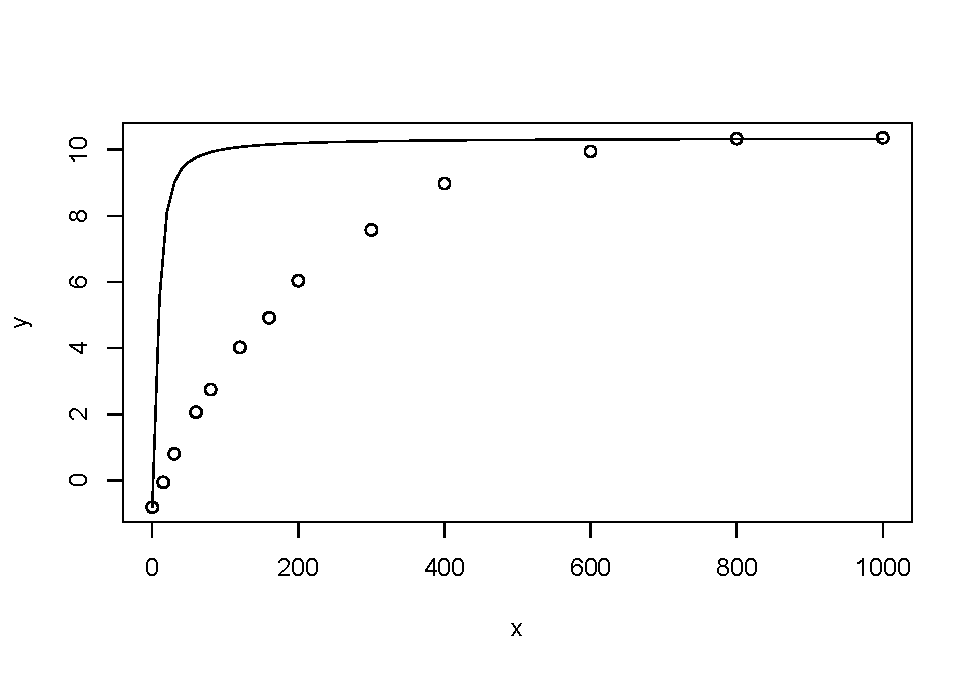
\includegraphics{bookdown_files/figure-latex/pomp-1.pdf}
\caption{\label{fig:pomp}初步判断 alpha 的初始值}
\end{figure}

观察上图 \ref{fig:pomp} 的结果可以看到,曲线在 0-600 的范围内,拟合值明显偏大,观察模型的方程式,以及其他起始值的设定方式,我们初步判断 alpha 的值偏大,于是乎我们将其改小观察,观察曲线和测量点的重合仍然不是很好,我们尝试修改 theta 值与 alpha 值(也即曲线高于测量点,则需要减小纵坐标的值,低于测量点,则需要增加该值,该过程省略,我大概设置了五分钟完成),最终得出的结果如下:

\begin{Shaded}
\begin{Highlighting}[]
\KeywordTok{plot}\NormalTok{(y }\OperatorTok{~}\StringTok{ }\NormalTok{x, }\DataTypeTok{data =}\NormalTok{ test)}
\KeywordTok{curve}\NormalTok{(}\KeywordTok{expfct}\NormalTok{(x, }\DataTypeTok{Am =}\NormalTok{ (}\KeywordTok{max}\NormalTok{(lrc_A)}\OperatorTok{-}\KeywordTok{min}\NormalTok{(lrc_A)),}
     \DataTypeTok{alpha=}\FloatTok{0.06}\NormalTok{, }\DataTypeTok{Rd=}\OperatorTok{-}\KeywordTok{min}\NormalTok{(lrc_A), }\DataTypeTok{theta=}\FloatTok{0.82}\NormalTok{), }\DataTypeTok{add =} \OtherTok{TRUE}\NormalTok{)}
\end{Highlighting}
\end{Shaded}

\begin{figure}
\centering
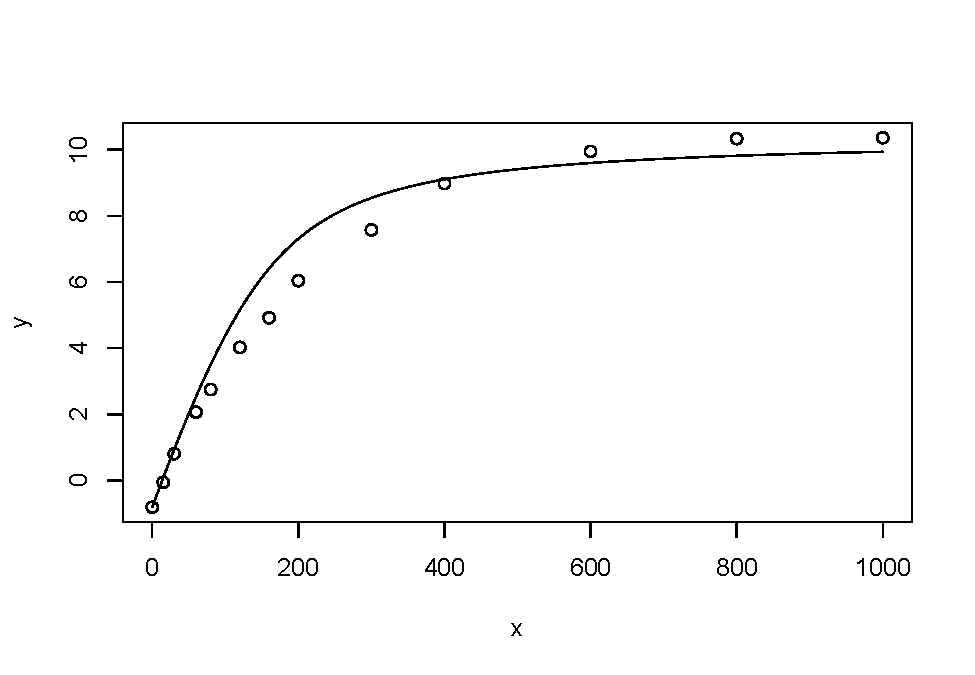
\includegraphics{bookdown_files/figure-latex/alpp-1.pdf}
\caption{\label{fig:alpp}初修正后断 alpha 的初始值}
\end{figure}

图 \ref{fig:alpp} 尽管看上去效果仍然不满意,但我们可试着进行拟合,看能否得到显著差异的结果:

\begin{Shaded}
\begin{Highlighting}[]
\NormalTok{lrcnls_manual <-}\StringTok{ }\KeywordTok{nls}\NormalTok{(lrc_A }\OperatorTok{~}\StringTok{ }
\StringTok{        }\NormalTok{(}\DecValTok{1}\OperatorTok{/}\NormalTok{(}\DecValTok{2}\OperatorTok{*}\NormalTok{theta))}\OperatorTok{*}
\StringTok{        }\NormalTok{(alpha}\OperatorTok{*}\NormalTok{lrc_Q}\OperatorTok{+}\NormalTok{Am}\OperatorTok{-}\KeywordTok{sqrt}\NormalTok{((alpha}\OperatorTok{*}\NormalTok{lrc_Q}\OperatorTok{+}\NormalTok{Am)}\OperatorTok{^}\DecValTok{2} \OperatorTok{-}\StringTok{ }
\StringTok{                               }\DecValTok{4}\OperatorTok{*}\NormalTok{alpha}\OperatorTok{*}\NormalTok{theta}\OperatorTok{*}\NormalTok{Am}\OperatorTok{*}\NormalTok{lrc_Q))}\OperatorTok{-}\StringTok{ }
\StringTok{        }\NormalTok{Rd, }\DataTypeTok{start=}\KeywordTok{list}\NormalTok{(}\DataTypeTok{Am=}\NormalTok{(}\KeywordTok{max}\NormalTok{(lrc_A)}\OperatorTok{-}\KeywordTok{min}\NormalTok{(lrc_A)),}
                       \DataTypeTok{alpha=}\FloatTok{0.03}\NormalTok{,}\DataTypeTok{Rd=}\OperatorTok{-}\KeywordTok{min}\NormalTok{(lrc_A),}\DataTypeTok{theta=}\FloatTok{0.6}\NormalTok{))}
\KeywordTok{summary}\NormalTok{(lrcnls_manual)}
\end{Highlighting}
\end{Shaded}

\begin{verbatim}
## 
## Formula: lrc_A ~ (1/(2 * theta)) * (alpha * lrc_Q + Am - sqrt((alpha * 
##     lrc_Q + Am)^2 - 4 * alpha * theta * Am * lrc_Q)) - Rd
## 
## Parameters:
##        Estimate Std. Error t value Pr(>|t|)    
## Am    12.307585   0.406741  30.259 2.30e-10 ***
## alpha  0.045706   0.003423  13.352 3.09e-07 ***
## Rd     0.656642   0.132646   4.950 0.000791 ***
## theta  0.707518   0.079739   8.873 9.59e-06 ***
## ---
## Signif. codes:  0 '***' 0.001 '**' 0.01 '*' 0.05 '.' 0.1 ' ' 1
## 
## Residual standard error: 0.1852 on 9 degrees of freedom
## 
## Number of iterations to convergence: 7 
## Achieved convergence tolerance: 4.601e-06
\end{verbatim}

\begin{Shaded}
\begin{Highlighting}[]
\CommentTok{# 对拟合之后的结果作图,观察使用我们的估计值,}
\CommentTok{# 迭代的最终值与元数据的重合程度}
\KeywordTok{plot}\NormalTok{(y }\OperatorTok{~}\StringTok{ }\NormalTok{x, }\DataTypeTok{data =}\NormalTok{ test, }\DataTypeTok{ylim =} \KeywordTok{c}\NormalTok{(}\OperatorTok{-}\DecValTok{2}\NormalTok{, }\DecValTok{14}\NormalTok{))}
\KeywordTok{curve}\NormalTok{(}\KeywordTok{expfct}\NormalTok{(x, }\DataTypeTok{Am =} \FloatTok{12.307586}\NormalTok{,}
     \DataTypeTok{alpha=}\FloatTok{0.045706}\NormalTok{, }\DataTypeTok{Rd=} \FloatTok{0.656643}\NormalTok{, }\DataTypeTok{theta=}\FloatTok{0.707518}\NormalTok{), }\DataTypeTok{add =} \OtherTok{TRUE}\NormalTok{)}
\end{Highlighting}
\end{Shaded}

\begin{figure}
\centering
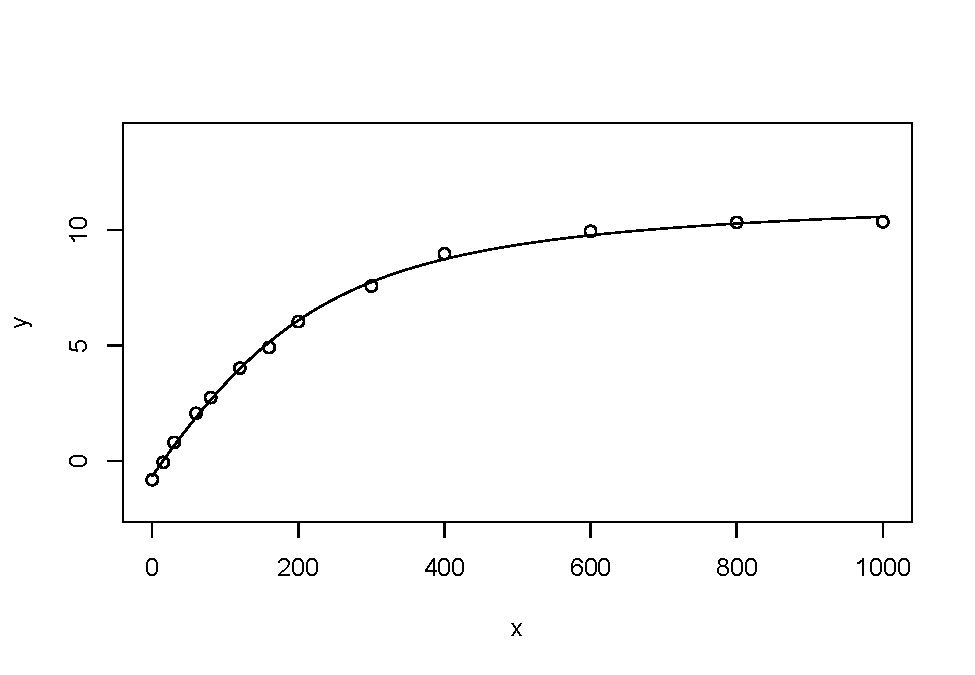
\includegraphics{bookdown_files/figure-latex/alpf-1.pdf}
\caption{\label{fig:alpf}检验作图法的初始值判断}
\end{figure}

从 \ref{fig:alpf} 的呈现以及 F 检验的 p 值来讲,图形已经比较完美了。\textbf{也就是说尽管我们作图的时候看到重合度并不高,但是非线性拟合本来就是一个迭代的过程,只要我们的数据与真实值相差不大,还是能够得到完美结果的}。

\hypertarget{show_demo}{%
\subsection{直观展示}\label{show_demo}}

上面的表述太啰嗦,直接用下面的图形说明一下,其中 alhpa 的取值在此处选择从 0.01 到 0.07,每次增加 0.05,其他值分别为 Am = 12.31, Rd= 0.66, theta=0.71 (此处为展示效果和方便,将这些值直接按照拟合结果设定了,实际差别不大)

\begin{Shaded}
\begin{Highlighting}[]
\KeywordTok{library}\NormalTok{(ggplot2)}
\KeywordTok{library}\NormalTok{(purrr)}

\NormalTok{lrc <-}\StringTok{ }\KeywordTok{read.csv}\NormalTok{(}\StringTok{"data/nlstest.csv"}\NormalTok{)}

\CommentTok{# 光响应曲线比较简单,我们将需要的数据直接提取,方便后面操作}
\NormalTok{lrc_Q <-}\StringTok{ }\NormalTok{lrc}\OperatorTok{$}\NormalTok{Qin}
\NormalTok{lrc_A <-}\StringTok{ }\NormalTok{lrc}\OperatorTok{$}\NormalTok{A}
\NormalTok{n <-}\StringTok{ }\KeywordTok{length}\NormalTok{(lrc_A)}


\NormalTok{alp <-}\StringTok{ }\KeywordTok{paste0}\NormalTok{(}\StringTok{"a="}\NormalTok{, }\KeywordTok{seq}\NormalTok{(}\FloatTok{0.01}\NormalTok{, }\FloatTok{0.07}\NormalTok{, }\DataTypeTok{by =} \FloatTok{0.005}\NormalTok{))}
\NormalTok{alpn <-}\StringTok{ }\KeywordTok{rep}\NormalTok{(alp, }\DataTypeTok{each =}\NormalTok{ n)}

\NormalTok{expfct <-}\StringTok{ }\ControlFlowTok{function}\NormalTok{(x, Am, alpha, Rd, theta) \{(}\DecValTok{1}\OperatorTok{/}\NormalTok{(}\DecValTok{2} \OperatorTok{*}\StringTok{ }\NormalTok{theta)) }\OperatorTok{*}\StringTok{ }\NormalTok{(alpha }\OperatorTok{*}\StringTok{ }\NormalTok{x }\OperatorTok{+}\StringTok{ }\NormalTok{Am }\OperatorTok{-}\StringTok{ }\KeywordTok{sqrt}\NormalTok{((alpha }\OperatorTok{*}\StringTok{ }\NormalTok{x }\OperatorTok{+}\StringTok{ }\NormalTok{Am)}\OperatorTok{^}\DecValTok{2} \OperatorTok{-}\StringTok{ }\DecValTok{4} \OperatorTok{*}\StringTok{ }\NormalTok{alpha }\OperatorTok{*}\StringTok{ }\NormalTok{theta }\OperatorTok{*}\StringTok{ }\NormalTok{Am }\OperatorTok{*}\StringTok{ }\NormalTok{x)) }\OperatorTok{-}\StringTok{ }\NormalTok{Rd}
\NormalTok{\}}

\NormalTok{paras <-}\StringTok{ }\KeywordTok{data.frame}\NormalTok{(}\DataTypeTok{alpha =} \KeywordTok{rep}\NormalTok{(}\KeywordTok{seq}\NormalTok{(}\FloatTok{0.01}\NormalTok{, }\FloatTok{0.07}\NormalTok{, }\DataTypeTok{by =} \FloatTok{0.005}\NormalTok{), }\DataTypeTok{each =}\NormalTok{ n), }
           \DataTypeTok{x =} \KeywordTok{rep}\NormalTok{(lrc_Q, n), }\DataTypeTok{Am =} \KeywordTok{rep}\NormalTok{(}\FloatTok{12.31}\NormalTok{, n), }\DataTypeTok{Rd =} \KeywordTok{rep}\NormalTok{(}\FloatTok{0.66}\NormalTok{, n), }
           \DataTypeTok{theta =} \KeywordTok{rep}\NormalTok{(}\FloatTok{0.71}\NormalTok{, n))}
\NormalTok{y =}\StringTok{ }\KeywordTok{unlist}\NormalTok{(}\KeywordTok{pmap}\NormalTok{(paras, expfct))}

\NormalTok{show <-}\StringTok{ }\KeywordTok{data.frame}\NormalTok{(}\DataTypeTok{x =} \KeywordTok{rep}\NormalTok{(lrc_Q, }\DecValTok{14}\NormalTok{),}
           \DataTypeTok{y =} \KeywordTok{c}\NormalTok{(lrc_A, y), }
           \DataTypeTok{a =} \KeywordTok{factor}\NormalTok{(}\KeywordTok{c}\NormalTok{(}\KeywordTok{rep}\NormalTok{(}\StringTok{"measured"}\NormalTok{, n), alpn),}
           \DataTypeTok{level =} \KeywordTok{c}\NormalTok{(}\StringTok{"measured"}\NormalTok{, alp)}
\NormalTok{             ))}

\KeywordTok{ggplot}\NormalTok{(}\DataTypeTok{data =}\NormalTok{ show, }\KeywordTok{aes}\NormalTok{(x, y, }\DataTypeTok{group =}\NormalTok{ a, }\DataTypeTok{color=}\NormalTok{a)) }\OperatorTok{+}\StringTok{ }
\StringTok{  }\KeywordTok{geom_point}\NormalTok{() }\OperatorTok{+}\StringTok{ }
\StringTok{  }\KeywordTok{geom_smooth}\NormalTok{(}\DataTypeTok{se =} \OtherTok{FALSE}\NormalTok{) }
\end{Highlighting}
\end{Shaded}

\begin{figure}
\centering
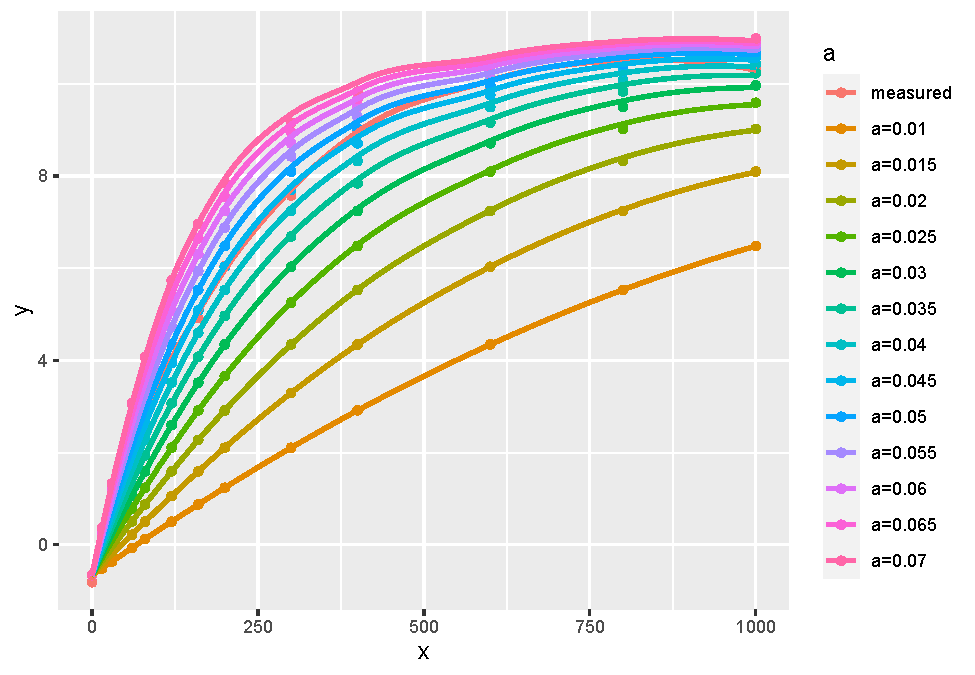
\includegraphics{bookdown_files/figure-latex/malp-1.pdf}
\caption{\label{fig:malp}多个 alpha 取值的差异}
\end{figure}

从上图 \ref{fig:malp} 我们我们可以看到,实测值在 alpha =0.04 和 alpha = 0.05 两条曲线之间,在 0.045 时最接近测量点,也就是我们把初始值设为 0.04 和 0.05 之间最接近,本例中可认为是0.045,实际这三个值均可。

\hypertarget{mult_try}{%
\section{自动多次尝试法}\label{mult_try}}

该方法实际为使用 \texttt{nls2} 来实现,具体方法参考 \citet{nls2} 的文章,可简单概括为使用一系列的起始值梯度(例如下面的代码中, alpha 的取值在 0.01 到 0.08 之间 ),然后软件循序使用不同的起始值,即排列组合所有的起始值序列,最终找到合适的值,具体实现如下:

\begin{Shaded}
\begin{Highlighting}[]
\KeywordTok{library}\NormalTok{(nls2)}
\end{Highlighting}
\end{Shaded}

\begin{verbatim}
## Loading required package: proto
\end{verbatim}

\begin{Shaded}
\begin{Highlighting}[]
\NormalTok{grid.test <-}\StringTok{ }\KeywordTok{expand.grid}\NormalTok{(}\KeywordTok{list}\NormalTok{(}
  \DataTypeTok{Am=}\KeywordTok{c}\NormalTok{(}\DecValTok{12}\NormalTok{),}
  \DataTypeTok{alpha =} \KeywordTok{seq}\NormalTok{(}\FloatTok{0.01}\NormalTok{, }\FloatTok{0.08}\NormalTok{, }\DataTypeTok{by =}\FloatTok{0.01}\NormalTok{),}
  \DataTypeTok{Rd =} \KeywordTok{seq}\NormalTok{(}\DecValTok{0}\NormalTok{, }\DecValTok{3}\NormalTok{),}
  \DataTypeTok{theta=}\KeywordTok{seq}\NormalTok{(}\FloatTok{0.1}\NormalTok{, }\DecValTok{1}\NormalTok{, }\DataTypeTok{by =} \FloatTok{0.1}\NormalTok{)}
\NormalTok{  ))}

\NormalTok{lrcnls2 <-}\StringTok{ }\KeywordTok{nls2}\NormalTok{(lrc_A }\OperatorTok{~}\StringTok{ }
\StringTok{        }\NormalTok{(}\DecValTok{1}\OperatorTok{/}\NormalTok{(}\DecValTok{2}\OperatorTok{*}\NormalTok{theta))}\OperatorTok{*}
\StringTok{        }\NormalTok{(alpha}\OperatorTok{*}\NormalTok{lrc_Q}\OperatorTok{+}\NormalTok{Am}\OperatorTok{-}\KeywordTok{sqrt}\NormalTok{((alpha}\OperatorTok{*}\NormalTok{lrc_Q}\OperatorTok{+}\NormalTok{Am)}\OperatorTok{^}\DecValTok{2} \OperatorTok{-}\StringTok{ }
\StringTok{                               }\DecValTok{4}\OperatorTok{*}\NormalTok{alpha}\OperatorTok{*}\NormalTok{theta}\OperatorTok{*}\NormalTok{Am}\OperatorTok{*}\NormalTok{lrc_Q))}\OperatorTok{-}\StringTok{ }
\StringTok{        }\NormalTok{Rd, }\DataTypeTok{start =}\NormalTok{ grid.test, }\DataTypeTok{algorithm =} \StringTok{"brute-force"}\NormalTok{)}
\end{Highlighting}
\end{Shaded}

\begin{verbatim}
## Error in numericDeriv(form[[3L]], names(ind), env) : 
##   Missing value or an infinity produced when evaluating the model
## Error in numericDeriv(form[[3L]], names(ind), env) : 
##   Missing value or an infinity produced when evaluating the model
## Error in numericDeriv(form[[3L]], names(ind), env) : 
##   Missing value or an infinity produced when evaluating the model
## Error in numericDeriv(form[[3L]], names(ind), env) : 
##   Missing value or an infinity produced when evaluating the model
## Error in numericDeriv(form[[3L]], names(ind), env) : 
##   Missing value or an infinity produced when evaluating the model
## Error in numericDeriv(form[[3L]], names(ind), env) : 
##   Missing value or an infinity produced when evaluating the model
## Error in numericDeriv(form[[3L]], names(ind), env) : 
##   Missing value or an infinity produced when evaluating the model
## Error in numericDeriv(form[[3L]], names(ind), env) : 
##   Missing value or an infinity produced when evaluating the model
## Error in numericDeriv(form[[3L]], names(ind), env) : 
##   Missing value or an infinity produced when evaluating the model
## Error in numericDeriv(form[[3L]], names(ind), env) : 
##   Missing value or an infinity produced when evaluating the model
## Error in numericDeriv(form[[3L]], names(ind), env) : 
##   Missing value or an infinity produced when evaluating the model
## Error in numericDeriv(form[[3L]], names(ind), env) : 
##   Missing value or an infinity produced when evaluating the model
## Error in numericDeriv(form[[3L]], names(ind), env) : 
##   Missing value or an infinity produced when evaluating the model
## Error in numericDeriv(form[[3L]], names(ind), env) : 
##   Missing value or an infinity produced when evaluating the model
## Error in numericDeriv(form[[3L]], names(ind), env) : 
##   Missing value or an infinity produced when evaluating the model
## Error in numericDeriv(form[[3L]], names(ind), env) : 
##   Missing value or an infinity produced when evaluating the model
\end{verbatim}

\begin{Shaded}
\begin{Highlighting}[]
\KeywordTok{summary}\NormalTok{(lrcnls2)}
\end{Highlighting}
\end{Shaded}

\begin{verbatim}
## 
## Formula: lrc_A ~ (1/(2 * theta)) * (alpha * lrc_Q + Am - sqrt((alpha * 
##     lrc_Q + Am)^2 - 4 * alpha * theta * Am * lrc_Q)) - Rd
## 
## Parameters:
##        Estimate Std. Error t value Pr(>|t|)    
## Am    12.000000   0.623023  19.261 1.27e-08 ***
## alpha  0.050000   0.006414   7.795 2.72e-05 ***
## Rd     1.000000   0.260153   3.844  0.00394 ** 
## theta  0.800000   0.102143   7.832 2.62e-05 ***
## ---
## Signif. codes:  0 '***' 0.001 '**' 0.01 '*' 0.05 '.' 0.1 ' ' 1
## 
## Residual standard error: 0.3663 on 9 degrees of freedom
## 
## Number of iterations to convergence: 320 
## Achieved convergence tolerance: NA
\end{verbatim}

通过结果可以看到,虽然和之前采用手动方法判定的结果比较接近,但是还是略有差异,可以看一下他们各自的结果同测量值的重合程度:

\begin{Shaded}
\begin{Highlighting}[]
\KeywordTok{plot}\NormalTok{(lrc_Q, lrc_A)}
\KeywordTok{lines}\NormalTok{(lrc_Q,  }\KeywordTok{predict}\NormalTok{(lrcnls2), }\DataTypeTok{col=}\StringTok{"red"}\NormalTok{)}
\KeywordTok{lines}\NormalTok{(lrc_Q,  }\KeywordTok{predict}\NormalTok{(lrcnls_manual), }\DataTypeTok{col=}\StringTok{"blue"}\NormalTok{)}
\end{Highlighting}
\end{Shaded}

\begin{figure}
\centering
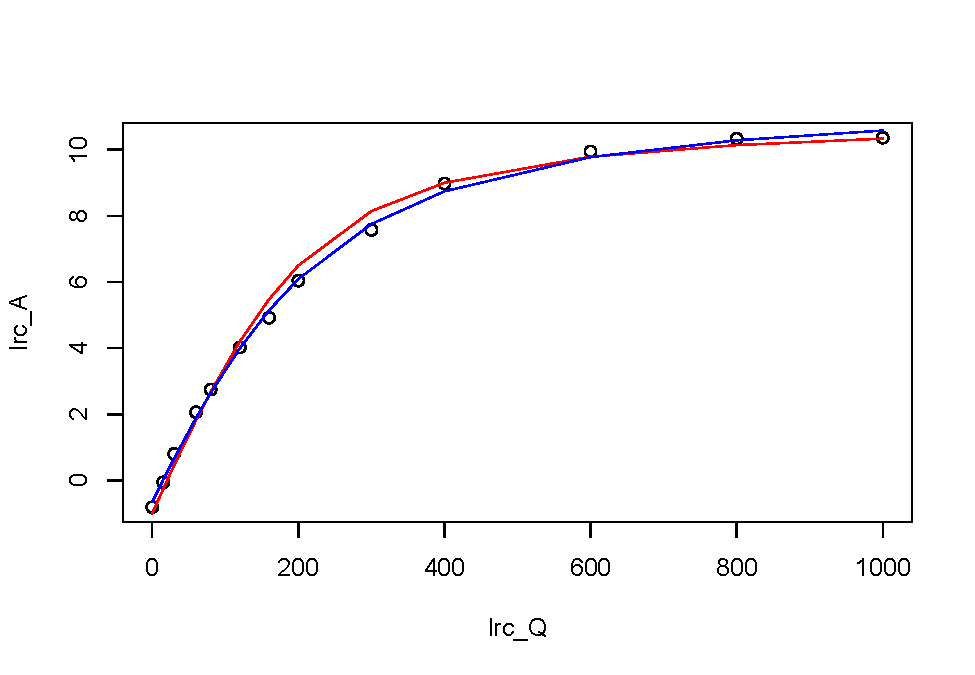
\includegraphics{bookdown_files/figure-latex/mcomp-1.pdf}
\caption{\label{fig:mcomp}两种方法结果的对比展示}
\end{figure}

图 \ref{fig:mcomp} 可以看到,使用 \texttt{nls2} 的拟合结果似乎和测量值更匹配,当然这只是第一印象,后续的判断还要进一步通过 F 检验、 AIC、BIC 等统计方式才能判定。

\hypertarget{sum_start}{%
\section{小结}\label{sum_start}}

采用如上三种方式都可以有效的解决起始值的问题,\texttt{nlsLM} 操作上更易实现,对初始值的大小不敏感,但设置不能太离谱,否则仍然会报错。作图比对法操作上更麻烦一些,但是这种方式一定能得出合理的初始值设置。采用 \texttt{nls2} 类似于将手动作图方式自动化,类似于 SPSS 中非线性拟合中需要给出一个初始值的范围,且该范围不能过大。如有一定的经验,操作起来将非常迅速。

需要注意的是,这三种方法结合起来使用会更好,例如,即使使用 \texttt{nlsLM} 的结果不合理,也可以参考他们参数的范围(部分结果也可能是差异显著),然后将这些结果用于手动作图判定参数或者 \texttt{nls2} 中判定参数范围,或者使用作图法确定大致的范围,将该范围输入到 \texttt{nls2} 中,这样会节省时间,也更加方便。

\cleardoublepage

\hypertarget{anay_6800}{%
\chapter{LI-6800 的数据分析}\label{anay_6800}}

\hypertarget{data6800}{%
\section{数据格式}\label{data6800}}

LI-6800 的数据前处理同 LI-6400 相同,如表 \ref{tab:head6800} 所示的样式。

\begin{longtable}{rrrlrr}
\caption{\label{tab:head6800}推荐 LI-6800 整理后数据样式}\\
\toprule
obs & time & elapsed & date & TIME & E\\
\midrule
1 & 1471425750 & 0.0 & 20160817 17:22:30 & 1471425726 & 0.0007614\\
2 & 1471425855 & 104.5 & 20160817 17:24:14 & 1471425829 & 0.0009221\\
3 & 1471426153 & 403.1 & 20160817 17:29:13 & 1471426144 & 0.0009900\\
4 & 1471426244 & 494.0 & 20160817 17:30:44 & 1471426235 & 0.0010249\\
5 & 1471426335 & 585.1 & 20160817 17:32:15 & 1471426326 & 0.0010632\\
\addlinespace
6 & 1471426426 & 676.0 & 20160817 17:33:46 & 1471426417 & 0.0011190\\
\bottomrule
\end{longtable}

\hypertarget{dif}{%
\section{LI-6800 与 LI-6400 使用时的差别}\label{dif}}

\texttt{plantecophys} 使用时建立在 LI-6400XT 基础之上的软件包,因此在 LI-6800 代码中,需要改动的是 fitaci、fitacis 及 fitBB 中的 varnames 选项,也就是将 LI-6400XT 的表头改为 LI-6800 的表头。
以 fitaci 函数为例:

\begin{Shaded}
\begin{Highlighting}[]
 \KeywordTok{fitaci}\NormalTok{(aci, }\DataTypeTok{varnames =} 
        \KeywordTok{list}\NormalTok{(}\DataTypeTok{ALEAF =} \StringTok{"A"}\NormalTok{, }\DataTypeTok{Tleaf =} \StringTok{"Tleaf"}\NormalTok{, }\DataTypeTok{Ci =} \StringTok{"Ci"}\NormalTok{, }
          \DataTypeTok{PPFD  =} \StringTok{"Qin"}\NormalTok{, }\DataTypeTok{Rd =} \StringTok{"Rd"}\NormalTok{))}
\end{Highlighting}
\end{Shaded}

\hypertarget{notice}{%
\section{光响应曲线注意事项}\label{notice}}

光响应曲线的拟合相对简单,仅需要光强和光合速率的值,其中需要修改的部分仅为光强的赋值部分,在文件名一致的前提下,修改如下代码即可:

\begin{Shaded}
\begin{Highlighting}[]
\NormalTok{lrc_Q <-}\StringTok{ }\NormalTok{lrc}\OperatorTok{$}\NormalTok{Qin}
\NormalTok{lrc_A <-}\StringTok{ }\NormalTok{lrc}\OperatorTok{$}\NormalTok{A }
\end{Highlighting}
\end{Shaded}

\hypertarget{racir68}{%
\section{\texorpdfstring{LI-6800 RACiR\texttrademark 的测量与拟合}{LI-6800 RACiR的测量与拟合}}\label{racir68}}

在评估作物性状时,V\(_{cmax}\) 及 J\(_{max}\)时非常有用,传统的 A--Ci 曲线测量要求植物叶片要在一定浓度 CO\(_{2}\)
下适应几分钟后完成测量,这样的测量有几个缺点:

\begin{itemize}
\tightlist
\item
  测量时间长,一条曲线至少需要 20 -- 30 min,样本量多,重复多时,这种方法几乎没有可行性。
\item
  整个测量过程中,时间长,酶的激活状态会有变化,叶绿体会移动,气孔的开度也会发生变化。
\end{itemize}

而 LI-6800 独有的 auto control 功能在算法上允许用户自定义 CO\(_{2}\) 的起始浓度和种植浓度、变化方式(线性或其他)、所花费的时间,再加上其
IRGAs 极快的响应频率,使得短时间内的 A--Ci 的测量成为现实,即快速 CO\(_{2}\) 响应曲线 RACiR\texttrademark
测量实验,该功能使得 5 min 内测量 A--Ci 曲线成为可能。该方法的实现可参考 \citet{stinziano2017}
的文章。

\citet{stinziano2018} 针对 RACiR\texttrademark 技术的疑问做了解答并提出了准确测量的建议,概括如下:

\begin{itemize}
\tightlist
\item
  首先,采用 100 ppm/min 的变化速率是与标准方法重合度最高的测量。
\item
  其次,明确研究问题,目前已有研究表明Vcmax 与 Jmax 的计算结果与标准测量方法结果无显著差异。
\item
  任何条件的改变,都需要做空叶室校准,例如:流速,气体浓度变化方向、温度,斜率等。
\item
  空叶室校准与叶片测量采用严格的同一次校准,因为 IRGA 的漂移,需要再次匹配时,或者环境条件改变时,需要重新做空叶室校准。是否需要匹配,可通过不加叶片的最初状态查看,此时 A 值应接近为0,reference 和 sample 气体浓度读数接近相等。
\item
  IRGA 分析器使用 5 此多项式进行校准,推荐使用 1 次到 5 次多项式进行拟合,然后根据 BIC 指数来确定最合适的空叶室校准系数(即非参数拟合的模型选择的问题)。
  确定最合适的浓度变化范围。通常需要去掉最初和最后 30 s的数据。
\item
  最小化校准和测量值之间的水分摩尔分数差异。甚至有可能需要控制 reference 或 sample 的水的摩尔分数而不是 Vpdleaf。
  通过预实验来确定最合适的 \(CO_2\) 变化范围和随时间的斜率。
\end{itemize}

\hypertarget{racir_pkg}{%
\section{\texorpdfstring{racir 软件包实现 RACiR\texttrademark 数据分析}{racir 软件包实现 RACiR数据分析}}\label{racir_pkg}}

\textbf{可能软件包作者没有更改叶面积的需求,他的软件包只支持原始数据的处理,但这对有更改需求的客户来讲没那么友好,而且这样导致了大量代码的重复,我根据作者原来的代码,结合我自己数据分析的习惯,重新制作了一份软件包,下面代码实现是基于我的软件包实现的,如有需求,也可使用作者原来的代码实现}

\begin{Shaded}
\begin{Highlighting}[]
\NormalTok{devtools}\OperatorTok{::}\KeywordTok{install_github}\NormalTok{(}\StringTok{"zhujiedong/racir"}\NormalTok{)}
\KeywordTok{library}\NormalTok{(racir)}
\end{Highlighting}
\end{Shaded}

软件包的函数很多,但可以分为下面几类:

\begin{itemize}
\item
  首先使用 \texttt{find\_cut} 来查看使用数据的范围(排除野点)。
\item
  使用 \texttt{racircheck} 来检查校正数据 (非必须,但建议进行数据质量检查)
\item
  使用 \texttt{racircal} 进行数据的校准
\end{itemize}

\hypertarget{racir_pkg_real}{%
\subsection{实现过程}\label{racir_pkg_real}}

手上暂时没有原始数据格式的 racir 数据,因而现在使用以前的 csv 数据进行操作(空叶室测量数据和带叶片测量数据转为 csv 格式)。

首先检查空叶室校准:

\begin{Shaded}
\begin{Highlighting}[]
\KeywordTok{library}\NormalTok{(racir)}
\CommentTok{# only check the empty chamber data here}
\NormalTok{em1 <-}\StringTok{ }\KeywordTok{read.csv}\NormalTok{(}\StringTok{"./data/racirem/em-1.csv"}\NormalTok{)}
\NormalTok{le1 <-}\StringTok{ }\KeywordTok{read.csv}\NormalTok{(}\StringTok{"./data/racirle/le-1.csv"}\NormalTok{)}
\KeywordTok{find_cut}\NormalTok{(em1)}
\end{Highlighting}
\end{Shaded}

\begin{figure}
\centering
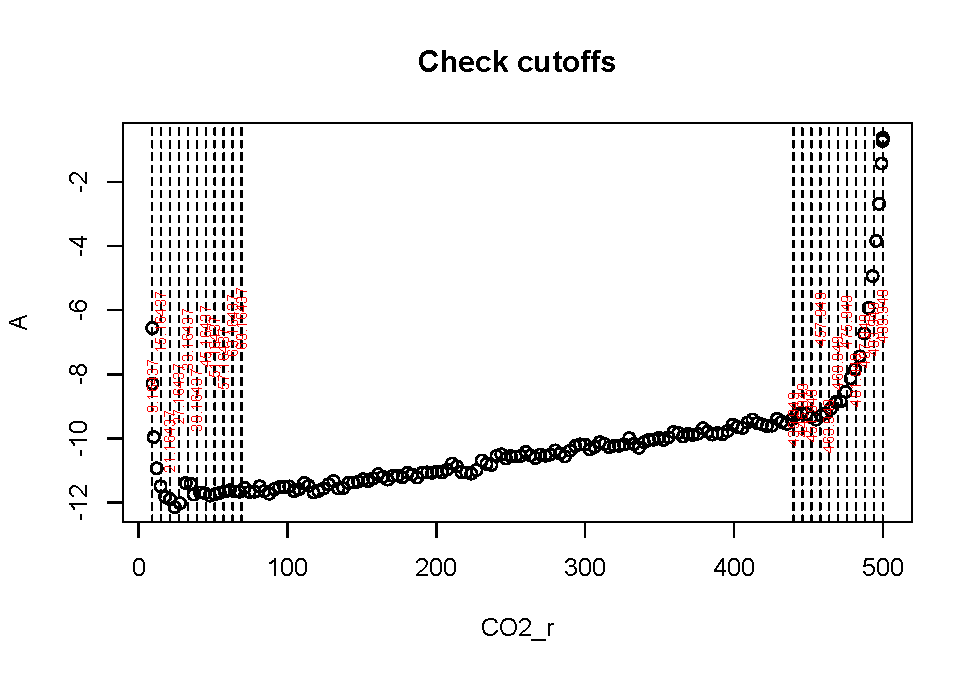
\includegraphics{bookdown_files/figure-latex/racircheck-1.pdf}
\caption{\label{fig:racircheck}找出最合理的校准曲线数据范围}
\end{figure}

上述代码查看参比室 \(CO_2\) 浓度在两者之间的数据,确定后面代码使用的 \texttt{mincut}, \texttt{maxcut} 范围。此处我选择的范围如下问代码:

\begin{Shaded}
\begin{Highlighting}[]
\KeywordTok{racircheck}\NormalTok{(em1, }\DataTypeTok{mincut =} \DecValTok{21}\NormalTok{ , }\DataTypeTok{maxcut =} \DecValTok{463}\NormalTok{ )}
\end{Highlighting}
\end{Shaded}

\begin{figure}
\centering
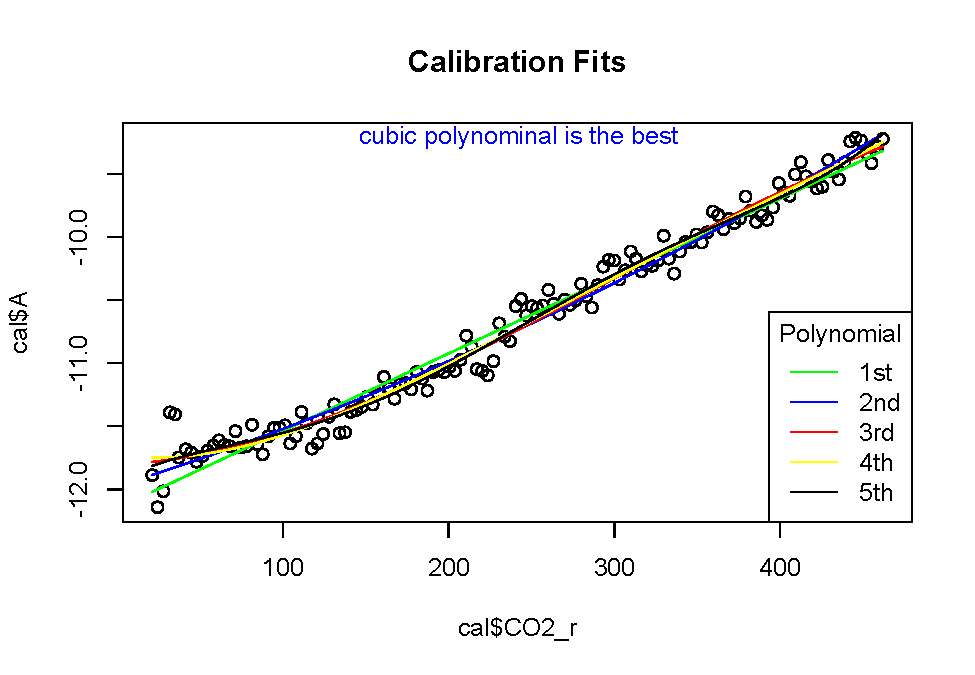
\includegraphics{bookdown_files/figure-latex/racircorpkg-1.pdf}
\caption{\label{fig:racircorpkg}校准曲线查看}
\end{figure}

没有问题可直接进行校准

\begin{Shaded}
\begin{Highlighting}[]
\NormalTok{x <-}\StringTok{ }\KeywordTok{racircal}\NormalTok{(em1, le1, }\DataTypeTok{mincut =} \DecValTok{21}\NormalTok{, }\DataTypeTok{maxcut =} \DecValTok{463}\NormalTok{)}
\KeywordTok{plot}\NormalTok{(x}\OperatorTok{$}\NormalTok{CO2_r, x}\OperatorTok{$}\NormalTok{A)}
\end{Highlighting}
\end{Shaded}

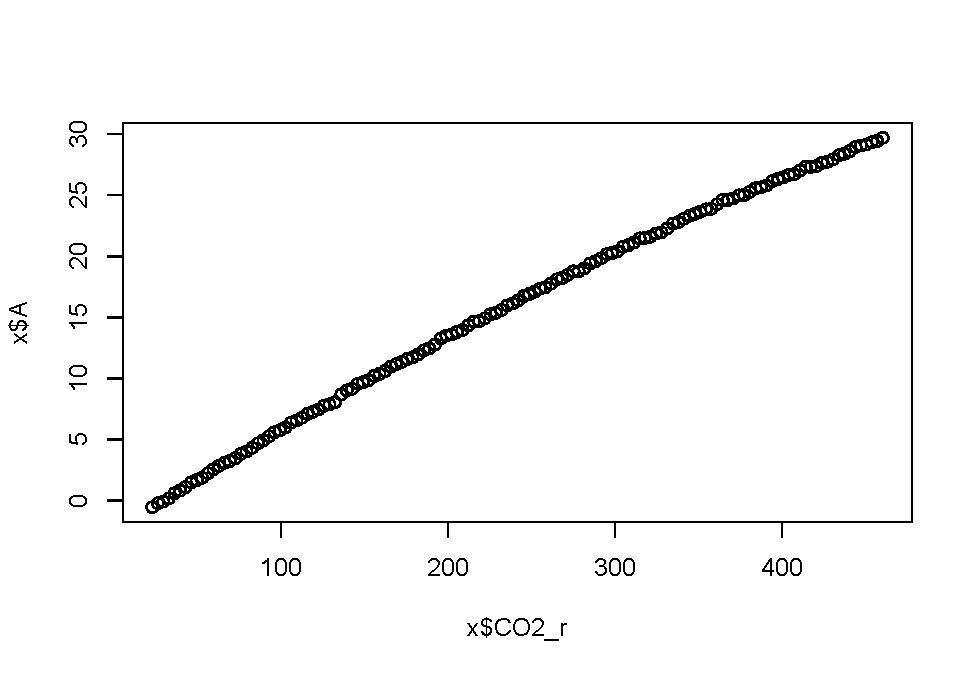
\includegraphics{bookdown_files/figure-latex/racircor-1.pdf}
前两个参数分别为空叶室数据,带叶片测量数据,后面的最大最小值为 \texttt{racircheck} 确定,剩余工作就是使用 \texttt{plantecophys} 进行分析,在此不再重复这个过程。

\textbf{注意:RACiR 的本意是表型研究中求 Vcmax 和 Jmax,因而,请忽略 Rd 等参数的计算结果}

\hypertarget{racirbatch}{%
\subsection{数据的批量处理}\label{racirbatch}}

\hypertarget{imbyphoto}{%
\subsubsection{readphoto 导入}\label{imbyphoto}}

如果数据的导入是使用 \texttt{readphoto} 批量处理,那么所在数据文件有 files 列,作为不同文件数据的区分,那么可以使用向量化处理方式实现数据的分析,参考如下代码:

\begin{Shaded}
\begin{Highlighting}[]
\KeywordTok{library}\NormalTok{(readphoto)}
\CommentTok{# read all empty data set}
\NormalTok{all_empty <-}\StringTok{ }\KeywordTok{read_bat_6800}\NormalTok{(}\StringTok{"./empty_data"}\NormalTok{)}
\CommentTok{# read all leaf data set}
\NormalTok{all_leaf <-}\StringTok{ }\KeywordTok{read_bat_6800}\NormalTok{(}\StringTok{"./leaf_data"}\NormalTok{)}
\NormalTok{listem  <-}\StringTok{  }\KeywordTok{split}\NormalTok{(all_empty, files)}
\NormalTok{listle <-}\StringTok{  }\KeywordTok{split}\NormalTok{(all_leaf, files)}
\NormalTok{cordata <-}\StringTok{ }\NormalTok{purrr}\OperatorTok{::}\KeywordTok{map2}\NormalTok{(listem, listle, racircal, }\DataTypeTok{mincut =} \DecValTok{21}\NormalTok{, }\DataTypeTok{maxcut =} \DecValTok{463}\NormalTok{)}
\end{Highlighting}
\end{Shaded}

所有的数据均保存在 cordata 中,特别注意 \textbf{此处要求 listem 与 listle 长度相同,因此,如果一个空叶室对多个带叶片测量数据,请将空叶室测量文件复制几份(注意对应顺序),使其每个带叶片测量的数据文件和空叶室测量数据文件数量相同,并且一一对应,例如 emtpy-1-1 数据文件对应 leaf-1-1},文件命名前即制定好命名规则,方便后续数据处理。

\hypertarget{imbycsv}{%
\subsubsection{处理大量 csv 文件}\label{imbycsv}}

\begin{Shaded}
\begin{Highlighting}[]
\CommentTok{# suppose leaf and empty data in 2 files in disk D:}
\NormalTok{le=}\KeywordTok{list.files}\NormalTok{(}\StringTok{"d:/racirle/"}\NormalTok{)}
\NormalTok{em=}\KeywordTok{list.files}\NormalTok{(}\StringTok{"d:/racirem/"}\NormalTok{)}

\CommentTok{# construct the path of these csv files}
\NormalTok{pathle =}\StringTok{ }\KeywordTok{paste0}\NormalTok{(}\StringTok{"d:/racirle/"}\NormalTok{, le)}
\NormalTok{pathem =}\StringTok{ }\KeywordTok{paste0}\NormalTok{(}\StringTok{"d:/racirem/"}\NormalTok{, em)}

\CommentTok{# import all leaf data and empty data separately}
\NormalTok{xx <-}\StringTok{ }\KeywordTok{lapply}\NormalTok{(pathle, read.csv)}
\NormalTok{yy <-}\StringTok{ }\KeywordTok{lapply}\NormalTok{(pathem, read.csv)}

\CommentTok{# correct all the data}
\NormalTok{all_correc <-}\StringTok{ }\NormalTok{purrr}\OperatorTok{::}\KeywordTok{map2}\NormalTok{(yy, xx, racircal, }\DataTypeTok{mincut =} \DecValTok{21}\NormalTok{, }\DataTypeTok{maxcut=}\DecValTok{463}\NormalTok{)}

\CommentTok{#  export all data to csv files, these file have the same name with leaf data}
\NormalTok{dirc <-}\StringTok{ }\KeywordTok{dir.create}\NormalTok{(}\StringTok{"d:/data/"}\NormalTok{)}
\NormalTok{finame <-}\StringTok{ "d:/data/"}
\NormalTok{finame <-}\StringTok{ }\KeywordTok{paste0}\NormalTok{(finame, le)}
\NormalTok{purrr}\OperatorTok{::}\KeywordTok{walk2}\NormalTok{(all_correc,  finame, write.csv)}
\end{Highlighting}
\end{Shaded}

以上代码仅供参考,主要是实现批量导入并校正,在批量将校正后数据导出为 csv 文件,为方便,将导出的文件名字命名为同原来带叶片测量数据相同的文件名,。

\hypertarget{fitbatracir}{%
\section{\texorpdfstring{批量计算 \(V_{cmax}\) 和 \(J_max\)}{批量计算 V\_\{cmax\} 和 J\_max}}\label{fitbatracir}}

\begin{Shaded}
\begin{Highlighting}[]
\CommentTok{#use csv data above}
\NormalTok{csvdata <-}\StringTok{ }\KeywordTok{lapply}\NormalTok{(all_correc, plantecophys}\OperatorTok{::}\NormalTok{fitaci, }
    \DataTypeTok{varnames =} \KeywordTok{list}\NormalTok{(}\DataTypeTok{ALEAF =} \StringTok{"A"}\NormalTok{, }\DataTypeTok{Tleaf =} \StringTok{"Tleaf"}\NormalTok{,}
    \DataTypeTok{Ci =} \StringTok{"Ci"}\NormalTok{, }\DataTypeTok{PPFD=} \StringTok{"Q"}\NormalTok{, }\DataTypeTok{Rd =} \StringTok{"Rd"}\NormalTok{), }\DataTypeTok{fitmethod =}\StringTok{"bilinear"}\NormalTok{)}

\CommentTok{# use readphoto data above}
\NormalTok{photodata <-}\StringTok{ }\KeywordTok{lapply}\NormalTok{(cordata, plantecophys}\OperatorTok{::}\NormalTok{fitaci, }
    \DataTypeTok{varnames =} \KeywordTok{list}\NormalTok{(}\DataTypeTok{ALEAF =} \StringTok{"A"}\NormalTok{, }\DataTypeTok{Tleaf =} \StringTok{"Tleaf"}\NormalTok{,}
    \DataTypeTok{Ci =} \StringTok{"Ci"}\NormalTok{, }\DataTypeTok{PPFD=} \StringTok{"Q"}\NormalTok{, }\DataTypeTok{Rd =} \StringTok{"Rd"}\NormalTok{), }\DataTypeTok{fitmethod =}\StringTok{"bilinear"}\NormalTok{)}
\end{Highlighting}
\end{Shaded}

批量分析同样使用向量化来进行,避免了循环,效率比较高,也可以将拟合结果 \texttt{coef} 中的 \(V_{cmax}\) 和 \(J_max\) 结果批量导入文件,参考 @\ref(imbycsv) 部分的代码。

\hypertarget{racir68_exam}{%
\section{\texorpdfstring{RACiR\texttrademark 分析的手动实现}{RACiR分析的手动实现}}\label{racir68_exam}}

以下内容是我之前写的内容,部分代码的实现和上述软件包相似,仅供参考,尤其是当您使用 \texttt{racir} 软件包报错时,可以参考下文代码手动实现 RACiR 数据的分析。

\begin{Shaded}
\begin{Highlighting}[]
\CommentTok{# 分别读取未校准空叶室数据}
\CommentTok{# 未校准带叶片测量数据}
\CommentTok{# 标准aci曲线测量数据}
\NormalTok{uemp500 <-}\StringTok{ }\KeywordTok{read.csv}\NormalTok{(}\StringTok{"./data/uncorr_emp500.csv"}\NormalTok{)}
\NormalTok{uleaf500 <-}\StringTok{ }\KeywordTok{read.csv}\NormalTok{(}\StringTok{"./data/uncorr_leaf500.csv"}\NormalTok{)}
\NormalTok{acin <-}\StringTok{ }\KeywordTok{read.csv}\NormalTok{(}\StringTok{"./data/aci_ex.csv"}\NormalTok{)}

\CommentTok{# 防止读入空白行}
\NormalTok{m <-}\StringTok{ }\KeywordTok{length}\NormalTok{(}\KeywordTok{which}\NormalTok{(uemp500}\OperatorTok{$}\NormalTok{obs }\OperatorTok{>=}\StringTok{ }\DecValTok{1}\NormalTok{))}
\NormalTok{n <-}\StringTok{ }\KeywordTok{length}\NormalTok{(}\KeywordTok{which}\NormalTok{(uleaf500}\OperatorTok{$}\NormalTok{obs }\OperatorTok{>=}\StringTok{ }\DecValTok{1}\NormalTok{))}
\NormalTok{uemp500 <-}\StringTok{ }\NormalTok{uemp500[}\DecValTok{1}\OperatorTok{:}\NormalTok{m,]}
\NormalTok{uleaf500 <-}\StringTok{ }\NormalTok{uleaf500[}\DecValTok{1}\OperatorTok{:}\NormalTok{n,]}

\CommentTok{# 观察空叶室未校准数据reference对A的图形}
\KeywordTok{plot}\NormalTok{(uemp500}\OperatorTok{$}\NormalTok{CO2_r, uemp500}\OperatorTok{$}\NormalTok{A)}
\CommentTok{# 选取线性部分用于校准}
\KeywordTok{locator}\NormalTok{()}
\CommentTok{# 执行locator命令后,在上图中的目标位置选点,}
\CommentTok{# 选好后按 esc 可以返回所选点的坐标(选点即为在}
\CommentTok{# 预期位置鼠标单击)}

\CommentTok{# 根据上面的点,利用二氧化碳的值过滤掉不需要的数据}
\CommentTok{# 只要在线性范围内选点,拟合结果相差很小}
\NormalTok{cemp <-}\StringTok{ }\NormalTok{uemp500[}\KeywordTok{which}\NormalTok{(uemp500}\OperatorTok{$}\NormalTok{CO2_r }\OperatorTok{>}\StringTok{ }
\StringTok{                        }\FloatTok{45.28} \OperatorTok{&}\StringTok{ }\NormalTok{uemp500}\OperatorTok{$}\NormalTok{CO2_r }\OperatorTok{<}\StringTok{ }\FloatTok{459.12}\NormalTok{),]}
\KeywordTok{plot}\NormalTok{(cemp}\OperatorTok{$}\NormalTok{CO2_r, cemp}\OperatorTok{$}\NormalTok{A)}

\CommentTok{# 采用 1~5 次多项式分别拟合}
\NormalTok{cal1st <-}\StringTok{ }\KeywordTok{lm}\NormalTok{(A }\OperatorTok{~}\StringTok{ }\NormalTok{CO2_r, }\DataTypeTok{data =}\NormalTok{ cemp)}
\NormalTok{cal2nd <-}\StringTok{ }\KeywordTok{lm}\NormalTok{(A }\OperatorTok{~}\StringTok{ }\KeywordTok{poly}\NormalTok{(CO2_r, }\DecValTok{2}\NormalTok{), }\DataTypeTok{data =}\NormalTok{ cemp)}
\NormalTok{cal3rd <-}\StringTok{ }\KeywordTok{lm}\NormalTok{(A }\OperatorTok{~}\StringTok{ }\KeywordTok{poly}\NormalTok{(CO2_r, }\DecValTok{3}\NormalTok{), }\DataTypeTok{data =}\NormalTok{ cemp)}
\NormalTok{cal4th <-}\StringTok{ }\KeywordTok{lm}\NormalTok{(A }\OperatorTok{~}\StringTok{ }\KeywordTok{poly}\NormalTok{(CO2_r, }\DecValTok{4}\NormalTok{), }\DataTypeTok{data =}\NormalTok{ cemp)}
\NormalTok{cal5th <-}\StringTok{ }\KeywordTok{lm}\NormalTok{(A }\OperatorTok{~}\StringTok{ }\KeywordTok{poly}\NormalTok{(CO2_r, }\DecValTok{5}\NormalTok{), }\DataTypeTok{data =}\NormalTok{ cemp)}

\CommentTok{# 利用 BIC 找出最合理的校准方程}
\NormalTok{bics <-}\StringTok{ }\KeywordTok{BIC}\NormalTok{(cal1st, cal2nd, cal3rd, cal4th, cal5th)}
\CommentTok{# noquote也就是没引号,成为名字}
\NormalTok{best <-}\StringTok{ }\KeywordTok{noquote}\NormalTok{(}\KeywordTok{rownames}\NormalTok{(bics)[bics}\OperatorTok{$}\NormalTok{BIC }\OperatorTok{==}\StringTok{ }\KeywordTok{min}\NormalTok{(bics}\OperatorTok{$}\NormalTok{BIC)])}
\NormalTok{best}

\CommentTok{# 校准带叶片测量的数据}
\NormalTok{uleafc <-}\StringTok{ }\NormalTok{uleaf500}
\NormalTok{uleafc}\OperatorTok{$}\NormalTok{A <-}\StringTok{ }\NormalTok{uleafc}\OperatorTok{$}\NormalTok{A }\OperatorTok{-}\StringTok{ }\KeywordTok{predict}\NormalTok{(cal4th, uleafc)}
\NormalTok{uleafc}\OperatorTok{$}\NormalTok{Ci <-}\StringTok{ }\NormalTok{((uleafc}\OperatorTok{$}\NormalTok{gtc }\OperatorTok{-}\StringTok{ }\NormalTok{uleafc}\OperatorTok{$}\NormalTok{E }\OperatorTok{/}\StringTok{ }\DecValTok{2}\NormalTok{) }\OperatorTok{*}\StringTok{ }\NormalTok{uleafc}\OperatorTok{$}\NormalTok{CO2_s }\OperatorTok{-}\StringTok{ }
\StringTok{                }\NormalTok{uleafc}\OperatorTok{$}\NormalTok{A) }\OperatorTok{/}\StringTok{ }\NormalTok{(uleafc}\OperatorTok{$}\NormalTok{gtc }\OperatorTok{+}\StringTok{ }\NormalTok{uleafc}\OperatorTok{$}\NormalTok{E }\OperatorTok{/}\StringTok{ }\DecValTok{2}\NormalTok{)}

\CommentTok{# 对校准前后的数据进行作图,查看校准效果}
\KeywordTok{plot}\NormalTok{(uleaf500}\OperatorTok{$}\NormalTok{CO2_r, uleaf500}\OperatorTok{$}\NormalTok{A, }\DataTypeTok{pch =} \DecValTok{2}\NormalTok{, }\DataTypeTok{ylim =} \KeywordTok{c}\NormalTok{(}\OperatorTok{-}\DecValTok{20}\NormalTok{, }\DecValTok{40}\NormalTok{))}
\KeywordTok{points}\NormalTok{(uleafc}\OperatorTok{$}\NormalTok{CO2_r, uleafc}\OperatorTok{$}\NormalTok{A)}
\KeywordTok{locator}\NormalTok{()}
\NormalTok{cleaf <-}\StringTok{ }\NormalTok{uleafc[}\KeywordTok{which}\NormalTok{(uleafc}\OperatorTok{$}\NormalTok{CO2_r }\OperatorTok{>}\StringTok{ }\FloatTok{16.6} \OperatorTok{&}\StringTok{ }
\StringTok{                        }\NormalTok{uleafc}\OperatorTok{$}\NormalTok{CO2_r }\OperatorTok{<}\StringTok{ }\DecValTok{478}\NormalTok{),]}
\KeywordTok{plot}\NormalTok{(cleaf}\OperatorTok{$}\NormalTok{CO2_r, cleaf}\OperatorTok{$}\NormalTok{A)}

\CommentTok{# 利用plantecophys拟合标准曲线和racir曲线}
\KeywordTok{library}\NormalTok{(}\StringTok{"plantecophys"}\NormalTok{)}
\NormalTok{acifit <-}\StringTok{ }\KeywordTok{fitaci}\NormalTok{(cleaf, }\DataTypeTok{varnames =} 
                   \KeywordTok{list}\NormalTok{(}\DataTypeTok{ALEAF =} \StringTok{"A"}\NormalTok{, }\DataTypeTok{Tleaf =} \StringTok{"Tleaf"}\NormalTok{, }\DataTypeTok{Ci =} \StringTok{"Ci"}\NormalTok{, }
                        \DataTypeTok{PPFD  =} \StringTok{"Qin"}\NormalTok{, }\DataTypeTok{Rd =} \StringTok{"Rd"}\NormalTok{), }\DataTypeTok{Patm =} \FloatTok{84.09}\NormalTok{)}
\NormalTok{acifit_normal <-}\StringTok{ }\KeywordTok{fitaci}\NormalTok{(acin, }\DataTypeTok{varnames =} 
                          \KeywordTok{list}\NormalTok{(}\DataTypeTok{ALEAF =} \StringTok{"A"}\NormalTok{, }\DataTypeTok{Tleaf =} \StringTok{"Tleaf"}\NormalTok{, }\DataTypeTok{Ci =} \StringTok{"Ci"}\NormalTok{, }
                               \DataTypeTok{PPFD  =} \StringTok{"Qin"}\NormalTok{, }\DataTypeTok{Rd =} \StringTok{"Rd"}\NormalTok{), }\DataTypeTok{Patm =} \FloatTok{84.09}\NormalTok{)}
\CommentTok{# 查看拟合数据}
\NormalTok{acifit}\OperatorTok{$}\NormalTok{pars}
\NormalTok{acifit_normal}\OperatorTok{$}\NormalTok{pars}

\CommentTok{# 对快速曲线作图拟合结果进行查看}
\KeywordTok{plot}\NormalTok{(acifit, }\DataTypeTok{linecols =} \KeywordTok{c}\NormalTok{(}\StringTok{"green"}\NormalTok{, }\StringTok{"blue"}\NormalTok{, }\StringTok{"red"}\NormalTok{))}

\CommentTok{#### ggplot2 作图}
\NormalTok{ddata <-}\StringTok{ }\NormalTok{acifit}\OperatorTok{$}\NormalTok{df}

\NormalTok{alldata <-}\StringTok{ }\KeywordTok{data.frame}\NormalTok{(}\DataTypeTok{A =} \KeywordTok{c}\NormalTok{(acin}\OperatorTok{$}\NormalTok{A, ddata}\OperatorTok{$}\NormalTok{Ac, ddata}\OperatorTok{$}\NormalTok{Aj, cleaf}\OperatorTok{$}\NormalTok{A), }
                      \DataTypeTok{Ci =} \KeywordTok{c}\NormalTok{(acin}\OperatorTok{$}\NormalTok{Ci, ddata}\OperatorTok{$}\NormalTok{Ci, ddata}\OperatorTok{$}\NormalTok{Ci, cleaf}\OperatorTok{$}\NormalTok{Ci),}
                      \DataTypeTok{Atype =} \KeywordTok{c}\NormalTok{(}
                        \KeywordTok{rep}\NormalTok{(}\StringTok{"standard Aci curve"}\NormalTok{, }\KeywordTok{length}\NormalTok{(acin}\OperatorTok{$}\NormalTok{A)),}
                        \KeywordTok{rep}\NormalTok{(}\StringTok{"Ac"}\NormalTok{, }\KeywordTok{length}\NormalTok{(ddata}\OperatorTok{$}\NormalTok{Ac)), }
                        \KeywordTok{rep}\NormalTok{(}\StringTok{"Aj"}\NormalTok{, }\KeywordTok{length}\NormalTok{(ddata}\OperatorTok{$}\NormalTok{Aj)),}
                        \KeywordTok{rep}\NormalTok{(}\StringTok{"A corrected"}\NormalTok{, }\KeywordTok{length}\NormalTok{(cleaf}\OperatorTok{$}\NormalTok{A))}
\NormalTok{                      )}
\NormalTok{)}

\NormalTok{alldata}\OperatorTok{$}\NormalTok{Atype <-}\StringTok{ }\KeywordTok{factor}\NormalTok{(alldata}\OperatorTok{$}\NormalTok{Atype, }
                        \DataTypeTok{levels =} \KeywordTok{c}\NormalTok{(}\StringTok{"standard Aci curve"}\NormalTok{, }
                                   \StringTok{"Ac"}\NormalTok{, }\StringTok{"Aj"}\NormalTok{, }\StringTok{"A corrected"}\NormalTok{))}

\KeywordTok{library}\NormalTok{(ggplot2)}
\NormalTok{p <-}\StringTok{ }\KeywordTok{ggplot}\NormalTok{(alldata)}
\NormalTok{p1 <-}\StringTok{ }\NormalTok{p }\OperatorTok{+}\StringTok{ }\KeywordTok{geom_point}\NormalTok{(}\KeywordTok{aes}\NormalTok{(Ci,A, }\DataTypeTok{colour =}\NormalTok{ Atype),  }\DataTypeTok{alpha =} \FloatTok{0.5}\NormalTok{)}

\NormalTok{p2 <-}\StringTok{ }\NormalTok{p1 }\OperatorTok{+}\StringTok{ }\KeywordTok{geom_smooth}\NormalTok{(}\KeywordTok{aes}\NormalTok{(Ci, A, }\DataTypeTok{colour =}\NormalTok{ Atype),}
                       \DataTypeTok{method =} \StringTok{'auto'}\NormalTok{) }\OperatorTok{+}\StringTok{ }
\StringTok{  }\KeywordTok{labs}\NormalTok{(}\DataTypeTok{y=}\KeywordTok{expression}\NormalTok{(}\KeywordTok{paste}\NormalTok{(}\StringTok{"A "}\NormalTok{, }\StringTok{"("}\NormalTok{, mu, }
\NormalTok{                          mol}\OperatorTok\NormalTok{m}\OperatorTok{^-}\DecValTok{2}\OperatorTok\NormalTok{s}\OperatorTok{^-}\DecValTok{1}\NormalTok{, }\StringTok{")"}\NormalTok{)), }
       \DataTypeTok{x=}\KeywordTok{expression}\NormalTok{(}\KeywordTok{paste}\NormalTok{(C[i], }\StringTok{" "}\NormalTok{,}
                          \StringTok{"("}\NormalTok{, mu, mol}\OperatorTok\NormalTok{mol}\OperatorTok{^-}\DecValTok{1}\NormalTok{, }\StringTok{")"}\NormalTok{)))}

\NormalTok{p2 }\OperatorTok{+}\StringTok{ }\KeywordTok{scale_x_continuous}\NormalTok{(}\DataTypeTok{limits=}\KeywordTok{c}\NormalTok{(}\DecValTok{0}\NormalTok{, }\DecValTok{1800}\NormalTok{),}
                        \DataTypeTok{breaks=}\KeywordTok{seq}\NormalTok{(}\DecValTok{0}\NormalTok{, }\DecValTok{1800}\NormalTok{, }\DecValTok{200}\NormalTok{)) }\OperatorTok{+}\StringTok{  }
\StringTok{  }\KeywordTok{scale_y_continuous}\NormalTok{(}\DataTypeTok{limits=}\KeywordTok{c}\NormalTok{(}\OperatorTok{-}\DecValTok{3}\NormalTok{, }\DecValTok{50}\NormalTok{),}
                     \DataTypeTok{breaks=}\KeywordTok{seq}\NormalTok{(}\DecValTok{0}\NormalTok{, }\DecValTok{50}\NormalTok{, }\DecValTok{10}\NormalTok{)) }\OperatorTok{+}\StringTok{ }
\StringTok{  }\KeywordTok{scale_colour_hue}\NormalTok{(}\DataTypeTok{name=}\StringTok{"  "}\NormalTok{, }
                   \DataTypeTok{labels=}\KeywordTok{c}\NormalTok{(}\StringTok{'ACi curve data; '}\NormalTok{, }
                            \KeywordTok{expression}\NormalTok{(}\KeywordTok{paste}\NormalTok{(A[c], }\StringTok{' data; '}\NormalTok{)), }
                            \KeywordTok{expression}\NormalTok{(}\KeywordTok{paste}\NormalTok{(A[j], }\StringTok{' data; '}\NormalTok{)), }
                            \StringTok{'RACiR data'}\NormalTok{) }
\NormalTok{  ) }\OperatorTok{+}\StringTok{ }\KeywordTok{theme_set}\NormalTok{(}\KeywordTok{theme_bw}\NormalTok{()) }\OperatorTok{+}
\StringTok{  }\KeywordTok{theme}\NormalTok{(}\DataTypeTok{axis.text.x  =} \KeywordTok{element_text}\NormalTok{(}\DataTypeTok{size =} \DecValTok{10}\NormalTok{, }
                                    \DataTypeTok{angle=}\DecValTok{30}\NormalTok{, }\DataTypeTok{vjust=}\FloatTok{0.5}\NormalTok{), }
        \DataTypeTok{axis.text.y =} \KeywordTok{element_text}\NormalTok{(}\DataTypeTok{size =} \DecValTok{10}\NormalTok{),}
        \DataTypeTok{axis.title.x =} \KeywordTok{element_text}\NormalTok{(}
          \DataTypeTok{size =} \DecValTok{12}\NormalTok{, }\DataTypeTok{face =} \StringTok{'bold'}\NormalTok{),}
        \DataTypeTok{axis.title.y =} \KeywordTok{element_text}\NormalTok{(}
          \DataTypeTok{size =} \DecValTok{12}\NormalTok{, }\DataTypeTok{face =} \StringTok{'bold'}\NormalTok{),}
        \DataTypeTok{legend.text.align =} \DecValTok{0}\NormalTok{,}
        \DataTypeTok{legend.position =} \KeywordTok{c}\NormalTok{(}\FloatTok{0.8}\NormalTok{, }\FloatTok{0.6}\NormalTok{))}
\end{Highlighting}
\end{Shaded}

最终采用常规方法和 RACiR\texttrademark 方法结果如图 \ref{fig:racir} 所示,其中 Aj 与 Ac 结果采用 RACiR\texttrademark 计算\footnote{注意,注意数据表头的大小写,此处代码中,为处理数据的方便,我更改了大小写,分析自己的数据时需要注意}。

\begin{figure}
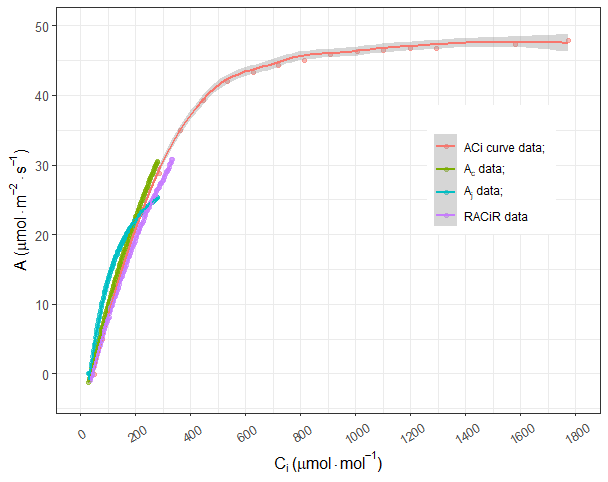
\includegraphics[width=1\linewidth]{images/racir} \caption{RACiR 方法与常规结果的比较}\label{fig:racir}
\end{figure}

\hypertarget{multirate-racir}{%
\section{利用不同速率的 RACiR 曲线研究植物的光合生理特性}\label{multirate-racir}}

自 RACiR 技术诞生以来,极大的缩短了 Vcmax 以及 Jmax 的测量时间(\citet{stinziano2017}),但也引起了一系列争议,作者也对业内的质疑进行了一一的解答 (\citet{stinziano2018}),但除了因为时间长短导致酶活性,叶绿体位置等差异外,RACiR 还能说明哪些问题呢?\citet{stinziano2019} 最新的研究给出一系列结论:

\begin{itemize}
\item
  扩散限制(\(CO_2\) 总导度) 和光呼吸导致了表观上的标准 ACi 曲线和 RACiR 测量之间的偏差,表明他们的差异是由\textbf{生物因子引起,而非仪器导致的人为误差}。
\item
  上述原因导致的二者之间的偏差,如果不进行修正,那么将显著的低估 \(\Gamma^*\), 除非使用多个速率的 RACiR 来修正。
\item
  较高速率的 RACiR 曲线会增大其与标准曲线之间的偏差,但这个差距在无光呼吸的条件下会减小。
\item
  因为光呼吸和气体扩散限制与物种相关,结合以上结论,可以使用多个速率的 RACiR 来估算对 \(CO_2\) 的总导度以及相对量的光呼吸速率。
\end{itemize}

一些可能的方向:

\begin{itemize}
\item
  扩散限制影响 Cc 速率的变化,说明对具有较高总阻力与 \(CO_2\) 比值的物种,例如针叶物种,C4 植物,较高的阻力导致 RACiR 与 标准 ACi 测量斜率更大的差异,或者测量的前提假设被破坏。
\item
  RACiR 可检测到代谢中 \(CO_2\) 的滞后性,各种滞后性的检测对标准 ACi 测量也具有指示性。
\end{itemize}

文中利用 R 实现了光呼吸之后模型和气体扩散限制模型,本文内容主要对文献中附录材料的源码进行解释:

\hypertarget{photoresp-lag}{%
\subsection{光呼吸滞后模型}\label{photoresp-lag}}

为测试光呼吸的滞后性,作者使用一系列预先设定的参数,模拟了一条 ACc曲线,假定 Rubisco 激活状态为 100\%,并且在整个测量过程中气孔导度是不变的。然后使用这些参数来模拟 RACiRs 曲线,并且假定光呼吸分别需要 0, 15, 30, 60, 120 或 300 s 来对变化的 \(CO_2\) 进行响应,在实际效果上,这意味着 Cc 在最初的 0, 15, 30, 60, 120 或 300 内是不变的,最后我们对 \(\Gamma^*\) 和 Ci 使用线性回归进行计算。

\hypertarget{base-data}{%
\subsubsection{基础数据}\label{base-data}}

模型第一步,则是对需要使用的参数,根据文献和实际情况进行赋值,具体内容参考代码注释。

\begin{Shaded}
\begin{Highlighting}[]
\KeywordTok{library}\NormalTok{(ggplot2)}
\KeywordTok{library}\NormalTok{(plyr)}
\end{Highlighting}
\end{Shaded}

\begin{verbatim}
## 
## Attaching package: 'plyr'
\end{verbatim}

\begin{verbatim}
## The following object is masked from 'package:purrr':
## 
##     compact
\end{verbatim}

\begin{Shaded}
\begin{Highlighting}[]
\KeywordTok{library}\NormalTok{(gridExtra)}

\CommentTok{# 对图例使用自定义颜色}
\NormalTok{gg_color_hue <-}\StringTok{ }\ControlFlowTok{function}\NormalTok{(n) \{}
\NormalTok{  hues =}\StringTok{ }\KeywordTok{seq}\NormalTok{(}\DecValTok{15}\NormalTok{, }\DecValTok{375}\NormalTok{, }\DataTypeTok{length =}\NormalTok{ n }\OperatorTok{+}\StringTok{ }\DecValTok{1}\NormalTok{)}
  \KeywordTok{hcl}\NormalTok{(}\DataTypeTok{h =}\NormalTok{ hues, }\DataTypeTok{l =} \DecValTok{65}\NormalTok{, }\DataTypeTok{c =} \DecValTok{100}\NormalTok{)[}\DecValTok{1}\OperatorTok{:}\NormalTok{n]}
\NormalTok{\}}

\CommentTok{#Maximum Rubisco carboxylation rate in umol m-2 s-1}
\NormalTok{Vcmax <-}\StringTok{ }\DecValTok{110}

\CommentTok{#Maximum Rubisco oxygenation rate in umol m-2 s-1;}
\CommentTok{#Ratio from Bernacchi et al. 2001. PCE 24:253-259}
\NormalTok{Vomax <-}\StringTok{ }\FloatTok{0.29} \OperatorTok{*}\StringTok{ }\NormalTok{Vcmax}
\CommentTok{#Dark respiration in umol m-2 s-1}
\NormalTok{R <-}\StringTok{ }\DecValTok{2}
\CommentTok{#Michaelis-Menten constant for Rubisco carboxylation in umol mol-1}
\NormalTok{Kc <-}\StringTok{ }\FloatTok{404.9}
\CommentTok{#Michaelis-Menten constant for Rubisco oxygenation in mmol mol-1}
\NormalTok{Ko <-}\StringTok{ }\FloatTok{278.4}
\CommentTok{#oxygen concentration in mmol mol-1}
\NormalTok{O2 <-}\StringTok{ }\DecValTok{210}
\NormalTok{Kco <-}\StringTok{ }\NormalTok{Kc }\OperatorTok{*}\StringTok{ }\NormalTok{(}\DecValTok{1} \OperatorTok{+}\StringTok{ }\NormalTok{O2 }\OperatorTok{/}\StringTok{ }\NormalTok{Ko)}
\CommentTok{#Boundary layer conductance in mol m-2 s-1}
\NormalTok{BLC <-}\StringTok{ }\DecValTok{2}
\CommentTok{#stomatal conductance in mol m-2 s-1}
\NormalTok{gsw <-}\StringTok{ }\FloatTok{0.4}
\CommentTok{#mesophyll conductance in mol m-2 s-1}
\NormalTok{gm <-}\StringTok{ }\DecValTok{1}
\CommentTok{#Chloroplastic CO2 in umol mol-1}
\NormalTok{Cc <-}\StringTok{ }\KeywordTok{as.numeric}\NormalTok{(}\KeywordTok{c}\NormalTok{(}\DecValTok{25}\OperatorTok{:}\DecValTok{400}\NormalTok{))}
\CommentTok{#oxygenation rate in umol m-2 s-1}
\NormalTok{vo <-}\StringTok{ }\NormalTok{Vomax }\OperatorTok{*}\StringTok{ }\NormalTok{O2 }\OperatorTok{/}\StringTok{ }\NormalTok{(O2 }\OperatorTok{+}\StringTok{ }\NormalTok{Ko }\OperatorTok{*}\StringTok{ }\NormalTok{(}\DecValTok{1} \OperatorTok{+}\StringTok{ }\NormalTok{Cc }\OperatorTok{/}\StringTok{ }\NormalTok{Kc))}
\CommentTok{#carboxylation rate in umol m-2 s-1}
\NormalTok{vc <-}\StringTok{ }\NormalTok{Vcmax }\OperatorTok{*}\StringTok{ }\NormalTok{(Cc) }\OperatorTok{/}\StringTok{ }\NormalTok{(Cc }\OperatorTok{+}\StringTok{ }\NormalTok{Kco)}
\CommentTok{#Net CO2 assimilation in umol m-2 s-1}
\NormalTok{A <-}\StringTok{ }\NormalTok{vc }\OperatorTok{-}\StringTok{ }\FloatTok{0.5} \OperatorTok{*}\StringTok{ }\NormalTok{vo }\OperatorTok{-}\StringTok{ }\NormalTok{R}
\CommentTok{#Apparent CO2 assimilation rate in umol m-2 s-1}
\NormalTok{Aapparent <-}\StringTok{ }\NormalTok{vc }\OperatorTok{-}\StringTok{ }\FloatTok{0.5} \OperatorTok{*}\StringTok{ }\NormalTok{vo}
\CommentTok{#Intercellular CO2 in umol mol-1}
\NormalTok{Ci <-}\StringTok{ }\NormalTok{A }\OperatorTok{/}\StringTok{ }\NormalTok{gm }\OperatorTok{+}\StringTok{ }\NormalTok{Cc}
\CommentTok{#Boundary layer CO2 in umol mol-1}
\NormalTok{Cb <-}\StringTok{ }\NormalTok{A }\OperatorTok{/}\StringTok{ }\NormalTok{gsw }\OperatorTok{+}\StringTok{ }\NormalTok{Ci}
\CommentTok{#Reference CO2 in umol mol-1}
\NormalTok{Cr <-}\StringTok{ }\NormalTok{A }\OperatorTok{/}\StringTok{ }\NormalTok{BLC }\OperatorTok{+}\StringTok{ }\NormalTok{Cb}

\CommentTok{#根据Cc浓度的个数,构造向量}
\NormalTok{Counter <-}\StringTok{ }\KeywordTok{as.numeric}\NormalTok{(}\KeywordTok{c}\NormalTok{(}\DecValTok{1}\OperatorTok{:}\KeywordTok{length}\NormalTok{(Cc)))}
\CommentTok{#也就是以秒计算的cr与时间的模型}
\NormalTok{RateCrmodel <-}\StringTok{ }\KeywordTok{lm}\NormalTok{(Cr }\OperatorTok{~}\StringTok{ }\NormalTok{Counter)}
\CommentTok{#转化为分钟的cr的斜率}
\NormalTok{RateCr <-}\StringTok{ }\KeywordTok{coef}\NormalTok{(RateCrmodel)[}\DecValTok{2}\NormalTok{] }\OperatorTok{*}\StringTok{ }\DecValTok{60}

\CommentTok{#转换为分钟的边界层导度斜率}
\NormalTok{RateCbmodel <-}\StringTok{ }\KeywordTok{lm}\NormalTok{(Cb }\OperatorTok{~}\StringTok{ }\NormalTok{Counter)}
\NormalTok{RateCb <-}\StringTok{ }\KeywordTok{coef}\NormalTok{(RateCbmodel)[}\DecValTok{2}\NormalTok{] }\OperatorTok{*}\StringTok{ }\DecValTok{60}

\CommentTok{#转换为分钟的ci的斜率}
\NormalTok{RateCimodel <-}\StringTok{ }\KeywordTok{lm}\NormalTok{(Ci }\OperatorTok{~}\StringTok{ }\NormalTok{Counter)}
\NormalTok{RateCi <-}\StringTok{ }\KeywordTok{coef}\NormalTok{(RateCimodel)[}\DecValTok{2}\NormalTok{] }\OperatorTok{*}\StringTok{ }\DecValTok{60}

\CommentTok{#转换为分钟的Cc的斜率}
\NormalTok{RateCcmodel <-}\StringTok{ }\KeywordTok{lm}\NormalTok{(Cc }\OperatorTok{~}\StringTok{ }\NormalTok{Counter)}
\NormalTok{RateCc <-}\StringTok{ }\KeywordTok{coef}\NormalTok{(RateCcmodel)[}\DecValTok{2}\NormalTok{] }\OperatorTok{*}\StringTok{ }\DecValTok{60} 
\end{Highlighting}
\end{Shaded}

\hypertarget{code-photoresp}{%
\subsection{光呼吸滞后性代码 \{code-photoresp\}}\label{code-photoresp}}

下面代码的目的是为得到 ACi 响应曲线受光呼吸延迟的影响,尤其是在临近补偿点时。

\textbf{延迟模块}

\begin{Shaded}
\begin{Highlighting}[]
\CommentTok{#假定有15s延迟时的数据,即相比上面构造的Cc数据减少15个点}
\NormalTok{Cc15 <-}\StringTok{ }\KeywordTok{as.numeric}\NormalTok{(}\KeywordTok{c}\NormalTok{((}\KeywordTok{min}\NormalTok{(Cc) }\OperatorTok{+}\StringTok{ }\DecValTok{15}\NormalTok{)}\OperatorTok{:}\KeywordTok{max}\NormalTok{(Cc), }\KeywordTok{rep}\NormalTok{(}\KeywordTok{max}\NormalTok{(Cc), }\DecValTok{15}\NormalTok{)))}
\NormalTok{vo15 <-}\StringTok{ }\NormalTok{Vomax }\OperatorTok{*}\StringTok{ }\NormalTok{O2 }\OperatorTok{/}\StringTok{ }\NormalTok{(O2 }\OperatorTok{+}\StringTok{ }\NormalTok{Ko }\OperatorTok{*}\StringTok{ }\NormalTok{(}\DecValTok{1} \OperatorTok{+}\StringTok{ }\NormalTok{Cc15 }\OperatorTok{/}\StringTok{ }\NormalTok{Kc))}
\NormalTok{A15 <-}\StringTok{ }\NormalTok{vc }\OperatorTok{-}\StringTok{ }\FloatTok{0.5} \OperatorTok{*}\StringTok{ }\NormalTok{vo15 }\OperatorTok{-}\StringTok{ }\NormalTok{R}
\NormalTok{Aapparent15 <-}\StringTok{ }\NormalTok{vc }\OperatorTok{-}\StringTok{ }\FloatTok{0.5} \OperatorTok{*}\StringTok{ }\NormalTok{vo15}

\CommentTok{#30 s 延迟数据}
\NormalTok{Cc30 <-}\StringTok{ }\KeywordTok{as.numeric}\NormalTok{(}\KeywordTok{c}\NormalTok{((}\KeywordTok{min}\NormalTok{(Cc) }\OperatorTok{+}\StringTok{ }\DecValTok{30}\NormalTok{)}\OperatorTok{:}\KeywordTok{max}\NormalTok{(Cc), }\KeywordTok{rep}\NormalTok{(}\KeywordTok{max}\NormalTok{(Cc), }\DecValTok{30}\NormalTok{)))}
\NormalTok{vo30 <-}\StringTok{ }\NormalTok{Vomax }\OperatorTok{*}\StringTok{ }\NormalTok{O2 }\OperatorTok{/}\StringTok{ }\NormalTok{(O2 }\OperatorTok{+}\StringTok{ }\NormalTok{Ko }\OperatorTok{*}\StringTok{ }\NormalTok{(}\DecValTok{1} \OperatorTok{+}\StringTok{ }\NormalTok{Cc30 }\OperatorTok{/}\StringTok{ }\NormalTok{Kc))}
\NormalTok{A30 <-}\StringTok{ }\NormalTok{vc }\OperatorTok{-}\StringTok{ }\FloatTok{0.5} \OperatorTok{*}\StringTok{ }\NormalTok{vo30 }\OperatorTok{-}\StringTok{ }\NormalTok{R}
\NormalTok{Aapparent30 <-}\StringTok{ }\NormalTok{vc }\OperatorTok{-}\StringTok{ }\FloatTok{0.5} \OperatorTok{*}\StringTok{ }\NormalTok{vo30}

\CommentTok{#60s 延迟数据}
\NormalTok{Cc60 <-}\StringTok{ }\KeywordTok{as.numeric}\NormalTok{(}\KeywordTok{c}\NormalTok{((}\KeywordTok{min}\NormalTok{(Cc) }\OperatorTok{+}\StringTok{ }\DecValTok{60}\NormalTok{)}\OperatorTok{:}\KeywordTok{max}\NormalTok{(Cc), }\KeywordTok{rep}\NormalTok{(}\KeywordTok{max}\NormalTok{(Cc), }\DecValTok{60}\NormalTok{)))}
\NormalTok{vo60 <-}\StringTok{ }\NormalTok{Vomax }\OperatorTok{*}\StringTok{ }\NormalTok{O2 }\OperatorTok{/}\StringTok{ }\NormalTok{(O2 }\OperatorTok{+}\StringTok{ }\NormalTok{Ko }\OperatorTok{*}\StringTok{ }\NormalTok{(}\DecValTok{1} \OperatorTok{+}\StringTok{ }\NormalTok{Cc60 }\OperatorTok{/}\StringTok{ }\NormalTok{Kc))}
\NormalTok{A60 <-}\StringTok{ }\NormalTok{vc }\OperatorTok{-}\StringTok{ }\FloatTok{0.5} \OperatorTok{*}\StringTok{ }\NormalTok{vo60 }\OperatorTok{-}\StringTok{ }\NormalTok{R}
\NormalTok{Aapparent60 <-}\StringTok{ }\NormalTok{vc }\OperatorTok{-}\StringTok{ }\FloatTok{0.5} \OperatorTok{*}\StringTok{ }\NormalTok{vo60}

\CommentTok{#120s延迟数据}
\NormalTok{Cc120 <-}\StringTok{ }\KeywordTok{as.numeric}\NormalTok{(}\KeywordTok{c}\NormalTok{((}\KeywordTok{min}\NormalTok{(Cc) }\OperatorTok{+}\StringTok{ }\DecValTok{120}\NormalTok{)}\OperatorTok{:}\KeywordTok{max}\NormalTok{(Cc), }\KeywordTok{rep}\NormalTok{(}\KeywordTok{max}\NormalTok{(Cc), }\DecValTok{120}\NormalTok{)))}
\NormalTok{vo120 <-}\StringTok{ }\NormalTok{Vomax }\OperatorTok{*}\StringTok{ }\NormalTok{O2 }\OperatorTok{/}\StringTok{ }\NormalTok{(O2 }\OperatorTok{+}\StringTok{ }\NormalTok{Ko }\OperatorTok{*}\StringTok{ }\NormalTok{(}\DecValTok{1} \OperatorTok{+}\StringTok{ }\NormalTok{Cc120 }\OperatorTok{/}\StringTok{ }\NormalTok{Kc))}
\NormalTok{A120 <-}\StringTok{ }\NormalTok{vc }\OperatorTok{-}\StringTok{ }\FloatTok{0.5} \OperatorTok{*}\StringTok{ }\NormalTok{vo120 }\OperatorTok{-}\StringTok{ }\NormalTok{R}
\NormalTok{Aapparent120 <-}\StringTok{ }\NormalTok{vc }\OperatorTok{-}\StringTok{ }\FloatTok{0.5} \OperatorTok{*}\StringTok{ }\NormalTok{vo120}

\CommentTok{#300s延迟数据}
\NormalTok{Cc300 <-}\StringTok{ }\KeywordTok{as.numeric}\NormalTok{(}\KeywordTok{c}\NormalTok{((}\KeywordTok{min}\NormalTok{(Cc) }\OperatorTok{+}\StringTok{ }\DecValTok{300}\NormalTok{)}\OperatorTok{:}\KeywordTok{max}\NormalTok{(Cc), }\KeywordTok{rep}\NormalTok{(}\KeywordTok{max}\NormalTok{(Cc), }\DecValTok{300}\NormalTok{)))}
\NormalTok{vo300 <-}\StringTok{ }\NormalTok{Vomax }\OperatorTok{*}\StringTok{ }\NormalTok{O2 }\OperatorTok{/}\StringTok{ }\NormalTok{(O2 }\OperatorTok{+}\StringTok{ }\NormalTok{Ko }\OperatorTok{*}\StringTok{ }\NormalTok{(}\DecValTok{1} \OperatorTok{+}\StringTok{ }\NormalTok{Cc300 }\OperatorTok{/}\StringTok{ }\NormalTok{Kc))}
\NormalTok{A300 <-}\StringTok{ }\NormalTok{vc }\OperatorTok{-}\StringTok{ }\FloatTok{0.5} \OperatorTok{*}\StringTok{ }\NormalTok{vo120 }\OperatorTok{-}\StringTok{ }\NormalTok{R}
\NormalTok{Aapparent300 <-}\StringTok{ }\NormalTok{vc }\OperatorTok{-}\StringTok{ }\FloatTok{0.5} \OperatorTok{*}\StringTok{ }\NormalTok{vo300 }
\end{Highlighting}
\end{Shaded}

\hypertarget{compi-modu}{%
\subsection{数据的构造}\label{compi-modu}}

下面的代码主要是将上文最终计算的数据构造数据集,并导出。

\begin{Shaded}
\begin{Highlighting}[]
\NormalTok{Anet <-}\StringTok{ }\KeywordTok{c}\NormalTok{(A, A15, A30, A60, A120, A300)}
\NormalTok{Aapp <-}
\StringTok{  }\KeywordTok{c}\NormalTok{(Aapparent,}
\NormalTok{    Aapparent15,}
\NormalTok{    Aapparent30,}
\NormalTok{    Aapparent60,}
\NormalTok{    Aapparent120,}
\NormalTok{    Aapparent300)}
\NormalTok{Ccfull <-}\StringTok{ }\KeywordTok{rep}\NormalTok{(Cc, }\DecValTok{6}\NormalTok{)}
\NormalTok{Cifull <-}\StringTok{ }\KeywordTok{rep}\NormalTok{(Ci, }\DecValTok{6}\NormalTok{)}
\NormalTok{Delay <-}
\StringTok{  }\KeywordTok{c}\NormalTok{(}
    \KeywordTok{rep}\NormalTok{(}\StringTok{"0"}\NormalTok{, }\KeywordTok{length}\NormalTok{(A)),}
    \KeywordTok{rep}\NormalTok{(}\StringTok{"15"}\NormalTok{, }\KeywordTok{length}\NormalTok{(A15)),}
    \KeywordTok{rep}\NormalTok{(}\StringTok{"30"}\NormalTok{, }\KeywordTok{length}\NormalTok{(A30)),}
    \KeywordTok{rep}\NormalTok{(}\StringTok{"60"}\NormalTok{, }\KeywordTok{length}\NormalTok{(A60)),}
    \KeywordTok{rep}\NormalTok{(}\StringTok{"120"}\NormalTok{, }\KeywordTok{length}\NormalTok{(A120)),}
    \KeywordTok{rep}\NormalTok{(}\StringTok{"300"}\NormalTok{, }\KeywordTok{length}\NormalTok{(A300))}
\NormalTok{  )}
\NormalTok{PRdata <-}\StringTok{ }\KeywordTok{as.data.frame}\NormalTok{(}\KeywordTok{cbind}\NormalTok{(Anet, Aapp, Ccfull, Cifull, Delay))}
\KeywordTok{write.csv}\NormalTok{(PRdata, }\StringTok{"./data/PRdata.csv"}\NormalTok{)}
\end{Highlighting}
\end{Shaded}

\hypertarget{photo-resp-graph}{%
\subsection{光呼吸滞后性作图}\label{photo-resp-graph}}

下面的代码是将光呼吸的数据进行作图。

\begin{Shaded}
\begin{Highlighting}[]
\NormalTok{data <-}\StringTok{ }\KeywordTok{read.csv}\NormalTok{(}\StringTok{"./data/PRdata.csv"}\NormalTok{)}
\NormalTok{data}\OperatorTok{$}\NormalTok{Ccfull <-}\StringTok{ }\KeywordTok{as.numeric}\NormalTok{(data}\OperatorTok{$}\NormalTok{Ccfull)}
\NormalTok{data}\OperatorTok{$}\NormalTok{Delay <-}\StringTok{ }\KeywordTok{as.factor}\NormalTok{(data}\OperatorTok{$}\NormalTok{Delay)}

\CommentTok{# 净光合速率与Cc作图}
\NormalTok{AnetCc <-}\StringTok{ }\KeywordTok{ggplot}\NormalTok{(data, }\KeywordTok{aes}\NormalTok{(}\DataTypeTok{x =}\NormalTok{ Ccfull, }\DataTypeTok{y =}\NormalTok{ Anet, }\DataTypeTok{colour =}\NormalTok{ Delay)) }\OperatorTok{+}
\StringTok{  }\KeywordTok{geom_point}\NormalTok{() }\OperatorTok{+}
\StringTok{  }\KeywordTok{labs}\NormalTok{(}\DataTypeTok{x =} \KeywordTok{expression}\NormalTok{(C[c] }\OperatorTok{~}\StringTok{ "("} \OperatorTok{*}\StringTok{ }\NormalTok{mu }\OperatorTok{*}\StringTok{ }\NormalTok{mol }\OperatorTok{~}\StringTok{ }\NormalTok{mol }\OperatorTok{^}\StringTok{ }\NormalTok{\{}
    \DecValTok{-1}
\NormalTok{  \} }\OperatorTok{*}\StringTok{ ")"}\NormalTok{),}
  \DataTypeTok{y =} \KeywordTok{expression}\NormalTok{(A[net] }\OperatorTok{~}\StringTok{ "("} \OperatorTok{*}\StringTok{ }\NormalTok{mu }\OperatorTok{*}\StringTok{ }\NormalTok{mol }\OperatorTok{~}\StringTok{ }\NormalTok{m }\OperatorTok{^}\StringTok{ }\NormalTok{\{}
    \DecValTok{-2}
\NormalTok{  \} }\OperatorTok{~}\StringTok{ }\NormalTok{s }\OperatorTok{^}\StringTok{ }\NormalTok{\{}
    \DecValTok{-1}
\NormalTok{  \} }\OperatorTok{*}\StringTok{ ")"}\NormalTok{)) }\OperatorTok{+}
\StringTok{  }\KeywordTok{labs}\NormalTok{(}\DataTypeTok{colour =} \StringTok{'Delay (s)'}\NormalTok{) }\OperatorTok{+}
\StringTok{  }\KeywordTok{scale_x_continuous}\NormalTok{(}\DataTypeTok{limits =} \KeywordTok{c}\NormalTok{(}\DecValTok{25}\NormalTok{, }\DecValTok{100}\NormalTok{),}
                     \DataTypeTok{breaks =} \KeywordTok{c}\NormalTok{(}\DecValTok{25}\NormalTok{, }\DecValTok{40}\NormalTok{, }\DecValTok{55}\NormalTok{, }\DecValTok{70}\NormalTok{, }\DecValTok{85}\NormalTok{, }\DecValTok{100}\NormalTok{)) }\OperatorTok{+}
\StringTok{  }\KeywordTok{scale_y_continuous}\NormalTok{(}\DataTypeTok{limits =} \KeywordTok{c}\NormalTok{(}\OperatorTok{-}\DecValTok{5}\NormalTok{, }\DecValTok{5}\NormalTok{)) }\OperatorTok{+}
\StringTok{  }\KeywordTok{scale_colour_brewer}\NormalTok{(}\DataTypeTok{palette =} \StringTok{'Spectral'}\NormalTok{) }\OperatorTok{+}
\StringTok{  }\CommentTok{#补偿点的参考线}
\StringTok{  }\KeywordTok{geom_hline}\NormalTok{(}\DataTypeTok{yintercept =} \DecValTok{0}\NormalTok{) }\OperatorTok{+}
\StringTok{  }\KeywordTok{theme_bw}\NormalTok{() }\OperatorTok{+}
\StringTok{  }\KeywordTok{theme}\NormalTok{(}\DataTypeTok{panel.grid.major =} \KeywordTok{element_blank}\NormalTok{(),}
        \DataTypeTok{panel.grid.minor =} \KeywordTok{element_blank}\NormalTok{())}
\NormalTok{AnetCc}
\end{Highlighting}
\end{Shaded}

\begin{figure}
\centering
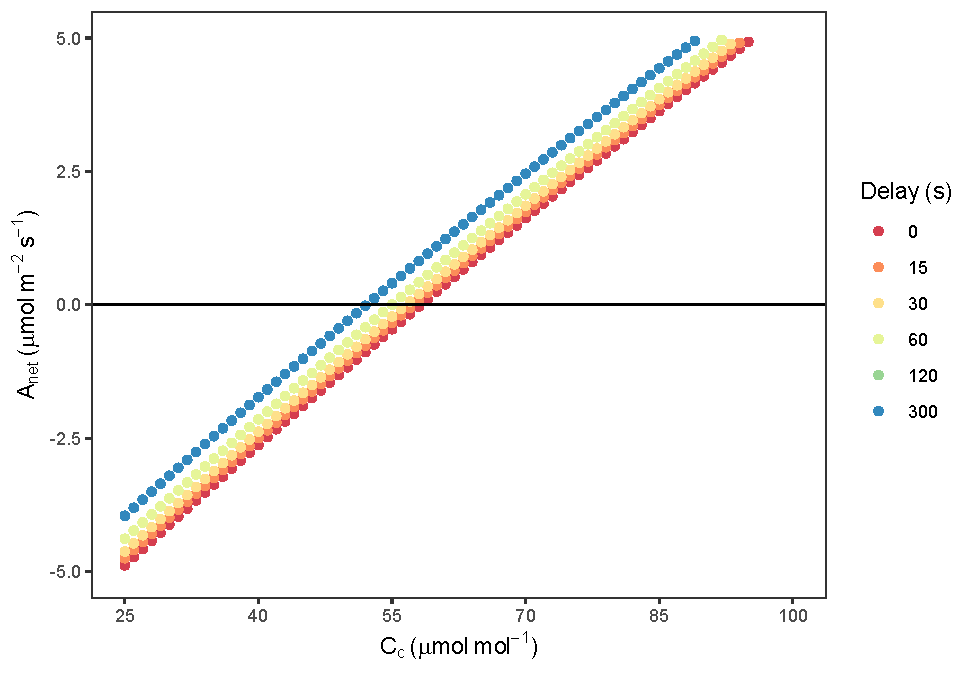
\includegraphics{bookdown_files/figure-latex/anetcc-1.pdf}
\caption{\label{fig:anetcc}Anet VS. Cc}
\end{figure}

\begin{Shaded}
\begin{Highlighting}[]
\CommentTok{#净光合速率与Ci作图}
\NormalTok{AnetCi <-}\StringTok{ }\KeywordTok{ggplot}\NormalTok{(data, }\KeywordTok{aes}\NormalTok{(}\DataTypeTok{x =}\NormalTok{ Cifull, }\DataTypeTok{y =}\NormalTok{ Anet, }\DataTypeTok{colour =}\NormalTok{ Delay)) }\OperatorTok{+}
\StringTok{  }\KeywordTok{geom_point}\NormalTok{() }\OperatorTok{+}
\StringTok{  }\KeywordTok{labs}\NormalTok{(}\DataTypeTok{x =} \KeywordTok{expression}\NormalTok{(C[i] }\OperatorTok{~}\StringTok{ "("} \OperatorTok{*}\StringTok{ }\NormalTok{mu }\OperatorTok{*}\StringTok{ }\NormalTok{mol }\OperatorTok{~}\StringTok{ }\NormalTok{mol }\OperatorTok{^}\StringTok{ }\NormalTok{\{}
    \DecValTok{-1}
\NormalTok{  \} }\OperatorTok{*}\StringTok{ ")"}\NormalTok{),}
  \DataTypeTok{y =} \KeywordTok{expression}\NormalTok{(A[net] }\OperatorTok{~}\StringTok{ "("} \OperatorTok{*}\StringTok{ }\NormalTok{mu }\OperatorTok{*}\StringTok{ }\NormalTok{mol }\OperatorTok{~}\StringTok{ }\NormalTok{m }\OperatorTok{^}\StringTok{ }\NormalTok{\{}
    \DecValTok{-2}
\NormalTok{  \} }\OperatorTok{~}\StringTok{ }\NormalTok{s }\OperatorTok{^}\StringTok{ }\NormalTok{\{}
    \DecValTok{-1}
\NormalTok{  \} }\OperatorTok{*}\StringTok{ ")"}\NormalTok{)) }\OperatorTok{+}
\StringTok{  }\KeywordTok{labs}\NormalTok{(}\DataTypeTok{colour =} \StringTok{'Delay (s)'}\NormalTok{) }\OperatorTok{+}
\StringTok{  }\KeywordTok{scale_x_continuous}\NormalTok{(}\DataTypeTok{limits =} \KeywordTok{c}\NormalTok{(}\DecValTok{25}\NormalTok{, }\DecValTok{100}\NormalTok{),}
                     \DataTypeTok{breaks =} \KeywordTok{c}\NormalTok{(}\DecValTok{25}\NormalTok{, }\DecValTok{40}\NormalTok{, }\DecValTok{55}\NormalTok{, }\DecValTok{70}\NormalTok{, }\DecValTok{85}\NormalTok{, }\DecValTok{100}\NormalTok{)) }\OperatorTok{+}
\StringTok{  }\KeywordTok{scale_y_continuous}\NormalTok{(}\DataTypeTok{limits =} \KeywordTok{c}\NormalTok{(}\OperatorTok{-}\DecValTok{5}\NormalTok{, }\DecValTok{5}\NormalTok{)) }\OperatorTok{+}
\StringTok{  }\KeywordTok{scale_colour_brewer}\NormalTok{(}\DataTypeTok{palette =} \StringTok{'Spectral'}\NormalTok{) }\OperatorTok{+}
\StringTok{  }\KeywordTok{geom_hline}\NormalTok{(}\DataTypeTok{yintercept =} \DecValTok{0}\NormalTok{) }\OperatorTok{+}
\StringTok{  }\KeywordTok{theme_bw}\NormalTok{() }\OperatorTok{+}
\StringTok{  }\KeywordTok{theme}\NormalTok{(}\DataTypeTok{panel.grid.major =} \KeywordTok{element_blank}\NormalTok{(),}
        \DataTypeTok{panel.grid.minor =} \KeywordTok{element_blank}\NormalTok{())}
\NormalTok{AnetCi}
\end{Highlighting}
\end{Shaded}

\begin{figure}
\centering
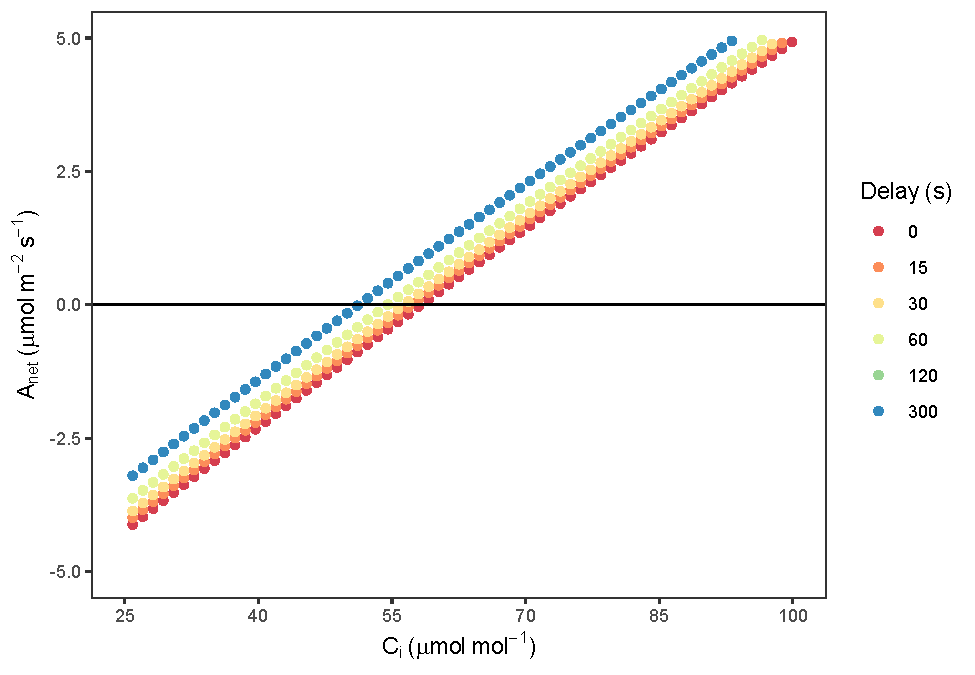
\includegraphics{bookdown_files/figure-latex/anetci-1.pdf}
\caption{\label{fig:anetci}Anet VS. Ci}
\end{figure}

\begin{Shaded}
\begin{Highlighting}[]
\CommentTok{#表观光合与Cc作图}
\NormalTok{AappCc <-}\StringTok{ }\KeywordTok{ggplot}\NormalTok{(data, }\KeywordTok{aes}\NormalTok{(}\DataTypeTok{x =}\NormalTok{ Ccfull, }\DataTypeTok{y =}\NormalTok{ Aapp, }\DataTypeTok{colour =}\NormalTok{ Delay)) }\OperatorTok{+}
\StringTok{  }\KeywordTok{geom_point}\NormalTok{() }\OperatorTok{+}
\StringTok{  }\KeywordTok{labs}\NormalTok{(}\DataTypeTok{x =} \KeywordTok{expression}\NormalTok{(C[c] }\OperatorTok{~}\StringTok{ "("} \OperatorTok{*}\StringTok{ }\NormalTok{mu }\OperatorTok{*}\StringTok{ }\NormalTok{mol }\OperatorTok{~}\StringTok{ }\NormalTok{mol }\OperatorTok{^}\StringTok{ }\NormalTok{\{}
    \DecValTok{-1}
\NormalTok{  \} }\OperatorTok{*}\StringTok{ ")"}\NormalTok{),}
  \DataTypeTok{y =} \KeywordTok{expression}\NormalTok{(A[apparent] }\OperatorTok{~}\StringTok{ "("} \OperatorTok{*}\StringTok{ }\NormalTok{mu }\OperatorTok{*}\StringTok{ }\NormalTok{mol }\OperatorTok{~}\StringTok{ }\NormalTok{m }\OperatorTok{^}\StringTok{ }\NormalTok{\{}
    \DecValTok{-2}
\NormalTok{  \} }\OperatorTok{~}\StringTok{ }\NormalTok{s }\OperatorTok{^}\StringTok{ }\NormalTok{\{}
    \DecValTok{-1}
\NormalTok{  \} }\OperatorTok{*}\StringTok{ ")"}\NormalTok{)) }\OperatorTok{+}
\StringTok{  }\KeywordTok{labs}\NormalTok{(}\DataTypeTok{colour =} \StringTok{'Delay (s)'}\NormalTok{) }\OperatorTok{+}
\StringTok{  }\KeywordTok{scale_x_continuous}\NormalTok{(}\DataTypeTok{limits =} \KeywordTok{c}\NormalTok{(}\DecValTok{25}\NormalTok{, }\DecValTok{75}\NormalTok{),}
                     \DataTypeTok{breaks =} \KeywordTok{c}\NormalTok{(}\DecValTok{25}\NormalTok{, }\DecValTok{35}\NormalTok{, }\DecValTok{45}\NormalTok{, }\DecValTok{55}\NormalTok{, }\DecValTok{65}\NormalTok{, }\DecValTok{75}\NormalTok{)) }\OperatorTok{+}
\StringTok{  }\KeywordTok{scale_y_continuous}\NormalTok{(}\DataTypeTok{limits =} \KeywordTok{c}\NormalTok{(}\OperatorTok{-}\DecValTok{5}\NormalTok{, }\DecValTok{5}\NormalTok{)) }\OperatorTok{+}
\StringTok{  }\KeywordTok{scale_colour_brewer}\NormalTok{(}\DataTypeTok{palette =} \StringTok{'Spectral'}\NormalTok{) }\OperatorTok{+}
\StringTok{  }\KeywordTok{geom_hline}\NormalTok{(}\DataTypeTok{yintercept =} \DecValTok{0}\NormalTok{) }\OperatorTok{+}
\StringTok{  }\KeywordTok{theme_bw}\NormalTok{() }\OperatorTok{+}
\StringTok{  }\KeywordTok{theme}\NormalTok{(}\DataTypeTok{panel.grid.major =} \KeywordTok{element_blank}\NormalTok{(),}
        \DataTypeTok{panel.grid.minor =} \KeywordTok{element_blank}\NormalTok{())}
\NormalTok{AappCc}
\end{Highlighting}
\end{Shaded}

\begin{figure}
\centering
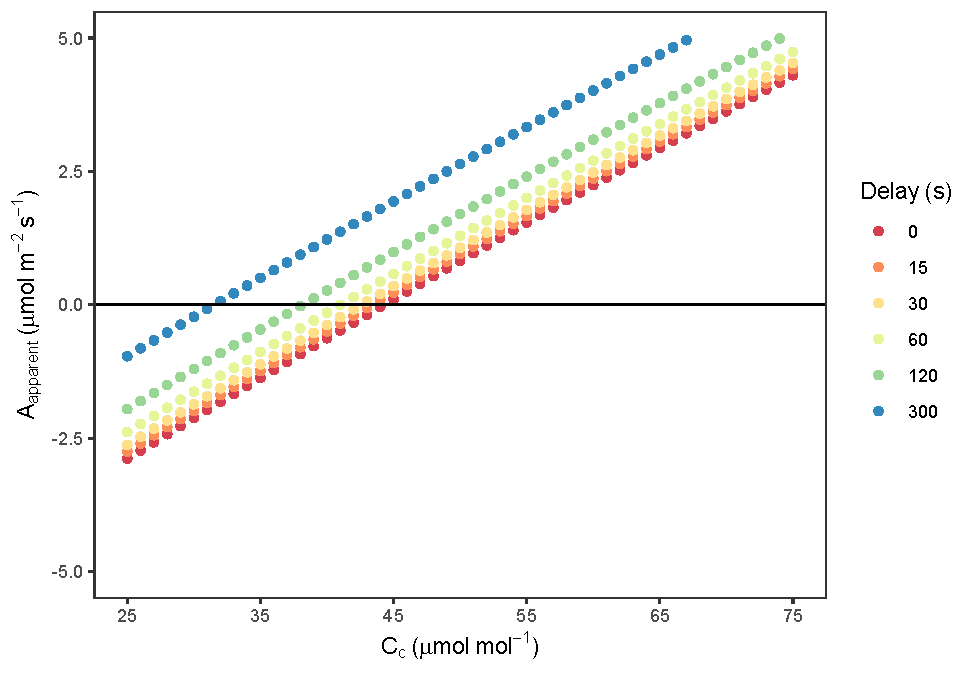
\includegraphics{bookdown_files/figure-latex/aappcc-1.pdf}
\caption{\label{fig:aappcc}Aapparent VS. Cc}
\end{figure}

\begin{Shaded}
\begin{Highlighting}[]
\CommentTok{#表观与Ci作图}
\NormalTok{AappCi <-}\StringTok{ }\KeywordTok{ggplot}\NormalTok{(data, }\KeywordTok{aes}\NormalTok{(}\DataTypeTok{x =}\NormalTok{ Cifull, }\DataTypeTok{y =}\NormalTok{ Aapp, }\DataTypeTok{colour =}\NormalTok{ Delay)) }\OperatorTok{+}
\StringTok{  }\KeywordTok{geom_point}\NormalTok{() }\OperatorTok{+}
\StringTok{  }\KeywordTok{labs}\NormalTok{(}\DataTypeTok{x =} \KeywordTok{expression}\NormalTok{(C[i] }\OperatorTok{~}\StringTok{ "("} \OperatorTok{*}\StringTok{ }\NormalTok{mu }\OperatorTok{*}\StringTok{ }\NormalTok{mol }\OperatorTok{~}\StringTok{ }\NormalTok{mol }\OperatorTok{^}\StringTok{ }\NormalTok{\{}
    \DecValTok{-1}
\NormalTok{  \} }\OperatorTok{*}\StringTok{ ")"}\NormalTok{),}
  \DataTypeTok{y =} \KeywordTok{expression}\NormalTok{(A[apparent] }\OperatorTok{~}\StringTok{ "("} \OperatorTok{*}\StringTok{ }\NormalTok{mu }\OperatorTok{*}\StringTok{ }\NormalTok{mol }\OperatorTok{~}\StringTok{ }\NormalTok{m }\OperatorTok{^}\StringTok{ }\NormalTok{\{}
    \DecValTok{-2}
\NormalTok{  \} }\OperatorTok{~}\StringTok{ }\NormalTok{s }\OperatorTok{^}\StringTok{ }\NormalTok{\{}
    \DecValTok{-1}
\NormalTok{  \} }\OperatorTok{*}\StringTok{ ")"}\NormalTok{)) }\OperatorTok{+}
\StringTok{  }\KeywordTok{labs}\NormalTok{(}\DataTypeTok{colour =} \StringTok{'Delay (s)'}\NormalTok{) }\OperatorTok{+}
\StringTok{  }\KeywordTok{scale_x_continuous}\NormalTok{(}\DataTypeTok{limits =} \KeywordTok{c}\NormalTok{(}\DecValTok{25}\NormalTok{, }\DecValTok{75}\NormalTok{),}
                     \DataTypeTok{breaks =} \KeywordTok{c}\NormalTok{(}\DecValTok{25}\NormalTok{, }\DecValTok{35}\NormalTok{, }\DecValTok{45}\NormalTok{, }\DecValTok{55}\NormalTok{, }\DecValTok{65}\NormalTok{, }\DecValTok{75}\NormalTok{)) }\OperatorTok{+}
\StringTok{  }\KeywordTok{scale_y_continuous}\NormalTok{(}\DataTypeTok{limits =} \KeywordTok{c}\NormalTok{(}\OperatorTok{-}\DecValTok{5}\NormalTok{, }\DecValTok{5}\NormalTok{)) }\OperatorTok{+}
\StringTok{  }\KeywordTok{scale_colour_brewer}\NormalTok{(}\DataTypeTok{palette =} \StringTok{'Spectral'}\NormalTok{) }\OperatorTok{+}
\StringTok{  }\KeywordTok{geom_hline}\NormalTok{(}\DataTypeTok{yintercept =} \DecValTok{0}\NormalTok{) }\OperatorTok{+}
\StringTok{  }\KeywordTok{theme_bw}\NormalTok{() }\OperatorTok{+}
\StringTok{  }\KeywordTok{theme}\NormalTok{(}\DataTypeTok{panel.grid.major =} \KeywordTok{element_blank}\NormalTok{(),}
        \DataTypeTok{panel.grid.minor =} \KeywordTok{element_blank}\NormalTok{())}
\NormalTok{AappCi}
\end{Highlighting}
\end{Shaded}

\begin{figure}
\centering
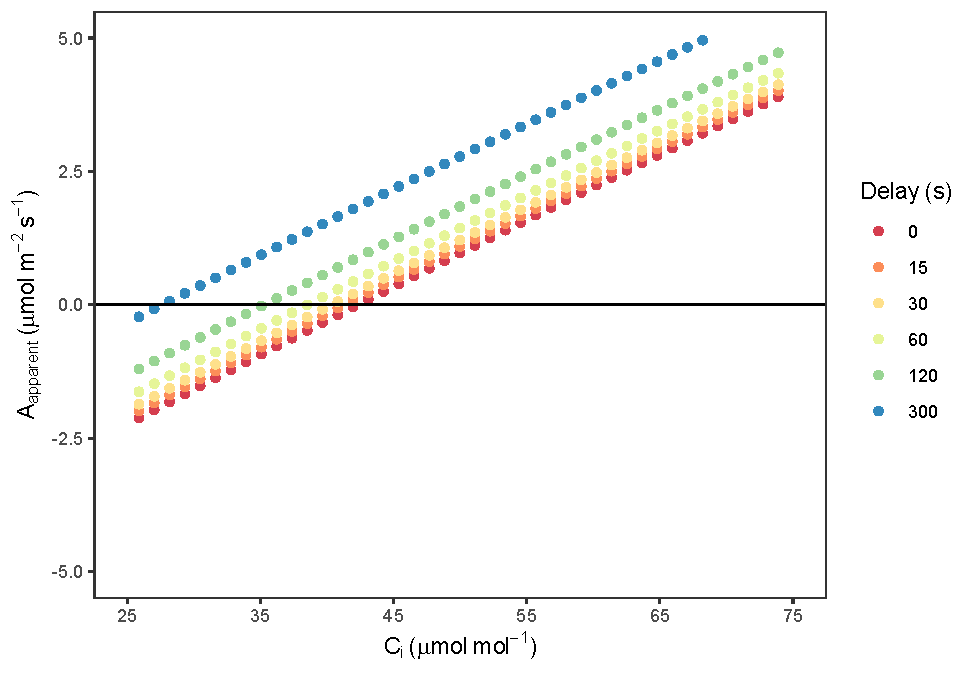
\includegraphics{bookdown_files/figure-latex/aappci-1.pdf}
\caption{\label{fig:aappci}Aapparent VS. Ci}
\end{figure}

\hypertarget{gammastar}{%
\subsection{补偿点计算}\label{gammastar}}

计算不同的光呼吸时间延迟下的补偿点(基于Ci):

\begin{Shaded}
\begin{Highlighting}[]
\CommentTok{#对于基于Ci的数据,仅采用ci<100时的数据}
\NormalTok{dataCi <-}\StringTok{ }\NormalTok{data[data}\OperatorTok{$}\NormalTok{Cifull }\OperatorTok{<}\StringTok{ }\DecValTok{100}\NormalTok{,]}
\NormalTok{dataCi0 <-}\StringTok{ }\NormalTok{dataCi[dataCi}\OperatorTok{$}\NormalTok{Delay }\OperatorTok{==}\StringTok{ "0"}\NormalTok{,]}
\NormalTok{dataCi15 <-}\StringTok{ }\NormalTok{dataCi[dataCi}\OperatorTok{$}\NormalTok{Delay }\OperatorTok{==}\StringTok{ "15"}\NormalTok{,]}
\NormalTok{dataCi30 <-}\StringTok{ }\NormalTok{dataCi[dataCi}\OperatorTok{$}\NormalTok{Delay }\OperatorTok{==}\StringTok{ "30"}\NormalTok{,]}
\NormalTok{dataCi60 <-}\StringTok{ }\NormalTok{dataCi[dataCi}\OperatorTok{$}\NormalTok{Delay }\OperatorTok{==}\StringTok{ "60"}\NormalTok{,]}
\NormalTok{dataCi120 <-}\StringTok{ }\NormalTok{dataCi[dataCi}\OperatorTok{$}\NormalTok{Delay }\OperatorTok{==}\StringTok{ "120"}\NormalTok{,]}
\NormalTok{dataCi300 <-}\StringTok{ }\NormalTok{dataCi[dataCi}\OperatorTok{$}\NormalTok{Delay }\OperatorTok{==}\StringTok{ "300"}\NormalTok{,]}

\CommentTok{#光呼吸无延迟时的计算,线性拟合}
\NormalTok{m1 <-}\StringTok{ }\KeywordTok{lm}\NormalTok{(dataCi0}\OperatorTok{$}\NormalTok{Anet }\OperatorTok{~}\StringTok{ }\NormalTok{dataCi0}\OperatorTok{$}\NormalTok{Cifull)}
\KeywordTok{summary}\NormalTok{(m1)}
\end{Highlighting}
\end{Shaded}

\begin{verbatim}
## 
## Call:
## lm(formula = dataCi0$Anet ~ dataCi0$Cifull)
## 
## Residuals:
##      Min       1Q   Median       3Q      Max 
## -0.13165 -0.04518  0.01711  0.05408  0.06699 
## 
## Coefficients:
##                  Estimate Std. Error t value Pr(>|t|)    
## (Intercept)    -7.2248105  0.0199353  -362.4   <2e-16 ***
## dataCi0$Cifull  0.1228632  0.0003089   397.8   <2e-16 ***
## ---
## Signif. codes:  0 '***' 0.001 '**' 0.01 '*' 0.05 '.' 0.1 ' ' 1
## 
## Residual standard error: 0.06081 on 69 degrees of freedom
## Multiple R-squared:  0.9996, Adjusted R-squared:  0.9996 
## F-statistic: 1.582e+05 on 1 and 69 DF,  p-value: < 2.2e-16
\end{verbatim}

\begin{Shaded}
\begin{Highlighting}[]
\CommentTok{#补偿点为截距比斜率(纵坐标为零)}
\NormalTok{Gamma0 <-}\StringTok{ }\OperatorTok{-}\NormalTok{m1}\OperatorTok{$}\NormalTok{coefficients[}\DecValTok{1}\NormalTok{] }\OperatorTok{/}\StringTok{ }\NormalTok{m1}\OperatorTok{$}\NormalTok{coefficients[}\DecValTok{2}\NormalTok{]}

\CommentTok{#光呼吸延时15s}
\NormalTok{m2 <-}\StringTok{ }\KeywordTok{lm}\NormalTok{(dataCi15}\OperatorTok{$}\NormalTok{Anet }\OperatorTok{~}\StringTok{ }\NormalTok{dataCi15}\OperatorTok{$}\NormalTok{Cifull)}
\KeywordTok{summary}\NormalTok{(m2)}
\end{Highlighting}
\end{Shaded}

\begin{verbatim}
## 
## Call:
## lm(formula = dataCi15$Anet ~ dataCi15$Cifull)
## 
## Residuals:
##      Min       1Q   Median       3Q      Max 
## -0.13119 -0.04502  0.01705  0.05389  0.06676 
## 
## Coefficients:
##                   Estimate Std. Error t value Pr(>|t|)    
## (Intercept)     -7.0873326  0.0198665  -356.7   <2e-16 ***
## dataCi15$Cifull  0.1225900  0.0003078   398.3   <2e-16 ***
## ---
## Signif. codes:  0 '***' 0.001 '**' 0.01 '*' 0.05 '.' 0.1 ' ' 1
## 
## Residual standard error: 0.0606 on 69 degrees of freedom
## Multiple R-squared:  0.9996, Adjusted R-squared:  0.9996 
## F-statistic: 1.586e+05 on 1 and 69 DF,  p-value: < 2.2e-16
\end{verbatim}

\begin{Shaded}
\begin{Highlighting}[]
\NormalTok{Gamma15 <-}\StringTok{ }\OperatorTok{-}\NormalTok{m2}\OperatorTok{$}\NormalTok{coefficients[}\DecValTok{1}\NormalTok{] }\OperatorTok{/}\StringTok{ }\NormalTok{m2}\OperatorTok{$}\NormalTok{coefficients[}\DecValTok{2}\NormalTok{]}

\CommentTok{#光呼吸延时30s}
\NormalTok{m3 <-}\StringTok{ }\KeywordTok{lm}\NormalTok{(dataCi30}\OperatorTok{$}\NormalTok{Anet }\OperatorTok{~}\StringTok{ }\NormalTok{dataCi30}\OperatorTok{$}\NormalTok{Cifull)}
\KeywordTok{summary}\NormalTok{(m3)}
\end{Highlighting}
\end{Shaded}

\begin{verbatim}
## 
## Call:
## lm(formula = dataCi30$Anet ~ dataCi30$Cifull)
## 
## Residuals:
##      Min       1Q   Median       3Q      Max 
## -0.13076 -0.04488  0.01699  0.05372  0.06654 
## 
## Coefficients:
##                   Estimate Std. Error t value Pr(>|t|)    
## (Intercept)     -6.9553180  0.0198028  -351.2   <2e-16 ***
## dataCi30$Cifull  0.1223321  0.0003068   398.7   <2e-16 ***
## ---
## Signif. codes:  0 '***' 0.001 '**' 0.01 '*' 0.05 '.' 0.1 ' ' 1
## 
## Residual standard error: 0.0604 on 69 degrees of freedom
## Multiple R-squared:  0.9996, Adjusted R-squared:  0.9996 
## F-statistic: 1.59e+05 on 1 and 69 DF,  p-value: < 2.2e-16
\end{verbatim}

\begin{Shaded}
\begin{Highlighting}[]
\NormalTok{Gamma30 <-}\StringTok{ }\OperatorTok{-}\NormalTok{m3}\OperatorTok{$}\NormalTok{coefficients[}\DecValTok{1}\NormalTok{] }\OperatorTok{/}\StringTok{ }\NormalTok{m3}\OperatorTok{$}\NormalTok{coefficients[}\DecValTok{2}\NormalTok{]}

\CommentTok{#光呼吸延时60s}
\NormalTok{m4 <-}\StringTok{ }\KeywordTok{lm}\NormalTok{(dataCi60}\OperatorTok{$}\NormalTok{Anet }\OperatorTok{~}\StringTok{ }\NormalTok{dataCi60}\OperatorTok{$}\NormalTok{Cifull)}
\KeywordTok{summary}\NormalTok{(m4)}
\end{Highlighting}
\end{Shaded}

\begin{verbatim}
## 
## Call:
## lm(formula = dataCi60$Anet ~ dataCi60$Cifull)
## 
## Residuals:
##      Min       1Q   Median       3Q      Max 
## -0.13001 -0.04462  0.01690  0.05341  0.06616 
## 
## Coefficients:
##                  Estimate Std. Error t value Pr(>|t|)    
## (Intercept)     -6.706429   0.019689  -340.6   <2e-16 ***
## dataCi60$Cifull  0.121858   0.000305   399.5   <2e-16 ***
## ---
## Signif. codes:  0 '***' 0.001 '**' 0.01 '*' 0.05 '.' 0.1 ' ' 1
## 
## Residual standard error: 0.06006 on 69 degrees of freedom
## Multiple R-squared:  0.9996, Adjusted R-squared:  0.9996 
## F-statistic: 1.596e+05 on 1 and 69 DF,  p-value: < 2.2e-16
\end{verbatim}

\begin{Shaded}
\begin{Highlighting}[]
\NormalTok{Gamma60 <-}\StringTok{ }\OperatorTok{-}\NormalTok{m4}\OperatorTok{$}\NormalTok{coefficients[}\DecValTok{1}\NormalTok{] }\OperatorTok{/}\StringTok{ }\NormalTok{m4}\OperatorTok{$}\NormalTok{coefficients[}\DecValTok{2}\NormalTok{]}

\CommentTok{#光呼吸延时120s}
\NormalTok{m5 <-}\StringTok{ }\KeywordTok{lm}\NormalTok{(dataCi120}\OperatorTok{$}\NormalTok{Anet }\OperatorTok{~}\StringTok{ }\NormalTok{dataCi120}\OperatorTok{$}\NormalTok{Cifull)}
\KeywordTok{summary}\NormalTok{(m5)}
\end{Highlighting}
\end{Shaded}

\begin{verbatim}
## 
## Call:
## lm(formula = dataCi120$Anet ~ dataCi120$Cifull)
## 
## Residuals:
##      Min       1Q   Median       3Q      Max 
## -0.12879 -0.04421  0.01673  0.05292  0.06555 
## 
## Coefficients:
##                    Estimate Std. Error t value Pr(>|t|)    
## (Intercept)      -6.2616980  0.0195062  -321.0   <2e-16 ***
## dataCi120$Cifull  0.1210486  0.0003022   400.5   <2e-16 ***
## ---
## Signif. codes:  0 '***' 0.001 '**' 0.01 '*' 0.05 '.' 0.1 ' ' 1
## 
## Residual standard error: 0.0595 on 69 degrees of freedom
## Multiple R-squared:  0.9996, Adjusted R-squared:  0.9996 
## F-statistic: 1.604e+05 on 1 and 69 DF,  p-value: < 2.2e-16
\end{verbatim}

\begin{Shaded}
\begin{Highlighting}[]
\NormalTok{Gamma120 <-}\StringTok{ }\OperatorTok{-}\NormalTok{m5}\OperatorTok{$}\NormalTok{coefficients[}\DecValTok{1}\NormalTok{] }\OperatorTok{/}\StringTok{ }\NormalTok{m5}\OperatorTok{$}\NormalTok{coefficients[}\DecValTok{2}\NormalTok{]}

\CommentTok{#光呼吸延时300s}
\NormalTok{m6 <-}\StringTok{ }\KeywordTok{lm}\NormalTok{(dataCi300}\OperatorTok{$}\NormalTok{Anet }\OperatorTok{~}\StringTok{ }\NormalTok{dataCi300}\OperatorTok{$}\NormalTok{Cifull)}
\KeywordTok{summary}\NormalTok{(m6)}
\end{Highlighting}
\end{Shaded}

\begin{verbatim}
## 
## Call:
## lm(formula = dataCi300$Anet ~ dataCi300$Cifull)
## 
## Residuals:
##      Min       1Q   Median       3Q      Max 
## -0.12879 -0.04421  0.01673  0.05292  0.06555 
## 
## Coefficients:
##                    Estimate Std. Error t value Pr(>|t|)    
## (Intercept)      -6.2616980  0.0195062  -321.0   <2e-16 ***
## dataCi300$Cifull  0.1210486  0.0003022   400.5   <2e-16 ***
## ---
## Signif. codes:  0 '***' 0.001 '**' 0.01 '*' 0.05 '.' 0.1 ' ' 1
## 
## Residual standard error: 0.0595 on 69 degrees of freedom
## Multiple R-squared:  0.9996, Adjusted R-squared:  0.9996 
## F-statistic: 1.604e+05 on 1 and 69 DF,  p-value: < 2.2e-16
\end{verbatim}

\begin{Shaded}
\begin{Highlighting}[]
\NormalTok{Gamma300 <-}\StringTok{ }\OperatorTok{-}\NormalTok{m6}\OperatorTok{$}\NormalTok{coefficients[}\DecValTok{1}\NormalTok{] }\OperatorTok{/}\StringTok{ }\NormalTok{m6}\OperatorTok{$}\NormalTok{coefficients[}\DecValTok{2}\NormalTok{]}
\end{Highlighting}
\end{Shaded}

构造数据并作图

\begin{Shaded}
\begin{Highlighting}[]
\NormalTok{GammaCi <-}\StringTok{ }\KeywordTok{c}\NormalTok{(Gamma0, Gamma15, Gamma30, Gamma60, Gamma120, Gamma300)}

\NormalTok{ints <-}
\StringTok{  }\KeywordTok{c}\NormalTok{(}
\NormalTok{    m1}\OperatorTok{$}\NormalTok{coefficients[}\DecValTok{1}\NormalTok{],}
\NormalTok{    m2}\OperatorTok{$}\NormalTok{coefficients[}\DecValTok{1}\NormalTok{],}
\NormalTok{    m3}\OperatorTok{$}\NormalTok{coefficients[}\DecValTok{1}\NormalTok{],}
\NormalTok{    m4}\OperatorTok{$}\NormalTok{coefficients[}\DecValTok{1}\NormalTok{],}
\NormalTok{    m5}\OperatorTok{$}\NormalTok{coefficients[}\DecValTok{1}\NormalTok{],}
\NormalTok{    m6}\OperatorTok{$}\NormalTok{coefficients[}\DecValTok{1}\NormalTok{]}
\NormalTok{  )}
\NormalTok{slps <-}
\StringTok{  }\KeywordTok{c}\NormalTok{(}
    \DecValTok{0}\NormalTok{,}
\NormalTok{    m2}\OperatorTok{$}\NormalTok{coefficients[}\DecValTok{2}\NormalTok{] }\OperatorTok{-}\StringTok{ }\NormalTok{m1}\OperatorTok{$}\NormalTok{coefficients[}\DecValTok{2}\NormalTok{],}
\NormalTok{    m3}\OperatorTok{$}\NormalTok{coefficients[}\DecValTok{2}\NormalTok{] }\OperatorTok{-}\StringTok{ }\NormalTok{m1}\OperatorTok{$}\NormalTok{coefficients[}\DecValTok{2}\NormalTok{],}
\NormalTok{    m4}\OperatorTok{$}\NormalTok{coefficients[}\DecValTok{2}\NormalTok{] }\OperatorTok{-}\StringTok{ }\NormalTok{m1}\OperatorTok{$}\NormalTok{coefficients[}\DecValTok{2}\NormalTok{],}
\NormalTok{    m5}\OperatorTok{$}\NormalTok{coefficients[}\DecValTok{2}\NormalTok{] }\OperatorTok{-}\StringTok{ }\NormalTok{m1}\OperatorTok{$}\NormalTok{coefficients[}\DecValTok{2}\NormalTok{],}
\NormalTok{    m6}\OperatorTok{$}\NormalTok{coefficients[}\DecValTok{2}\NormalTok{] }\OperatorTok{-}\StringTok{ }\NormalTok{m1}\OperatorTok{$}\NormalTok{coefficients[}\DecValTok{2}\NormalTok{]}
\NormalTok{  )}
\NormalTok{dels <-}\StringTok{ }\KeywordTok{c}\NormalTok{(}\DecValTok{0}\NormalTok{, }\DecValTok{15}\NormalTok{, }\DecValTok{30}\NormalTok{, }\DecValTok{60}\NormalTok{, }\DecValTok{120}\NormalTok{, }\DecValTok{300}\NormalTok{)}
\KeywordTok{summary}\NormalTok{(}\KeywordTok{lm}\NormalTok{(ints }\OperatorTok{~}\StringTok{ }\NormalTok{dels))}
\end{Highlighting}
\end{Shaded}

\begin{verbatim}
## 
## Call:
## lm(formula = ints ~ dels)
## 
## Residuals:
##   (Intercept) (Intercept).1 (Intercept).2 (Intercept).3 (Intercept).4 
##      -0.20351      -0.11262      -0.02719       0.12853       0.38691 
## (Intercept).5 
##      -0.17212 
## 
## Coefficients:
##               Estimate Std. Error t value Pr(>|t|)    
## (Intercept) -7.0213001  0.1343090 -52.277 8.01e-07 ***
## dels         0.0031057  0.0009959   3.119   0.0356 *  
## ---
## Signif. codes:  0 '***' 0.001 '**' 0.01 '*' 0.05 '.' 0.1 ' ' 1
## 
## Residual standard error: 0.2503 on 4 degrees of freedom
## Multiple R-squared:  0.7086, Adjusted R-squared:  0.6357 
## F-statistic: 9.725 on 1 and 4 DF,  p-value: 0.03558
\end{verbatim}

\begin{Shaded}
\begin{Highlighting}[]
\KeywordTok{plot}\NormalTok{(ints }\OperatorTok{~}\StringTok{ }\NormalTok{dels)}
\end{Highlighting}
\end{Shaded}

\begin{figure}
\centering
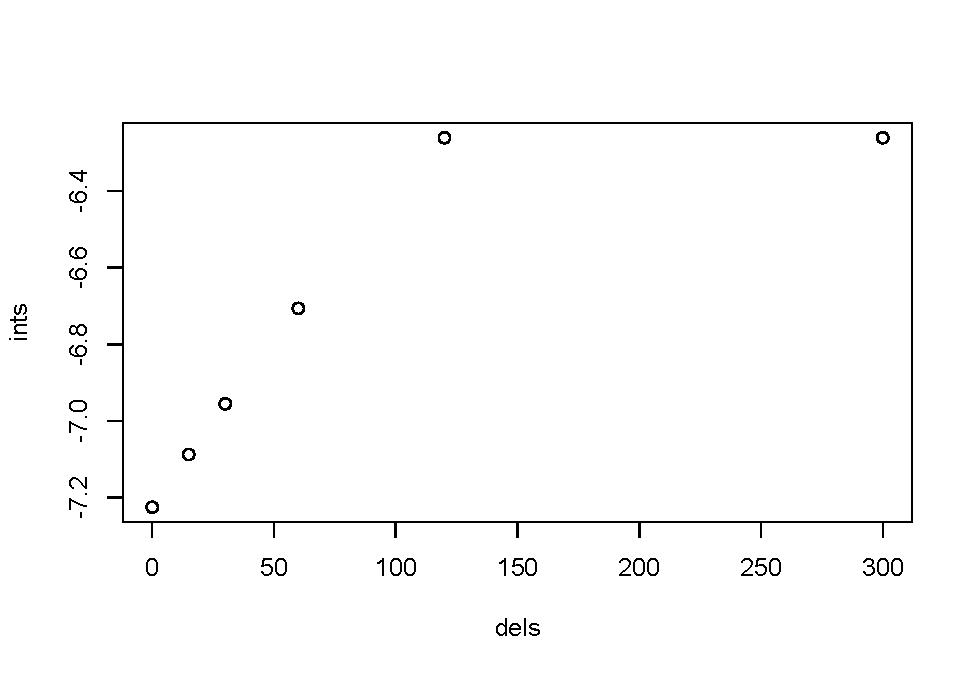
\includegraphics{bookdown_files/figure-latex/intdelay-1.pdf}
\caption{\label{fig:intdelay}基于 Ci 的不同延时下的截距}
\end{figure}

\begin{Shaded}
\begin{Highlighting}[]
\KeywordTok{plot}\NormalTok{(slps }\OperatorTok{~}\StringTok{ }\NormalTok{dels)}
\end{Highlighting}
\end{Shaded}

\begin{figure}
\centering
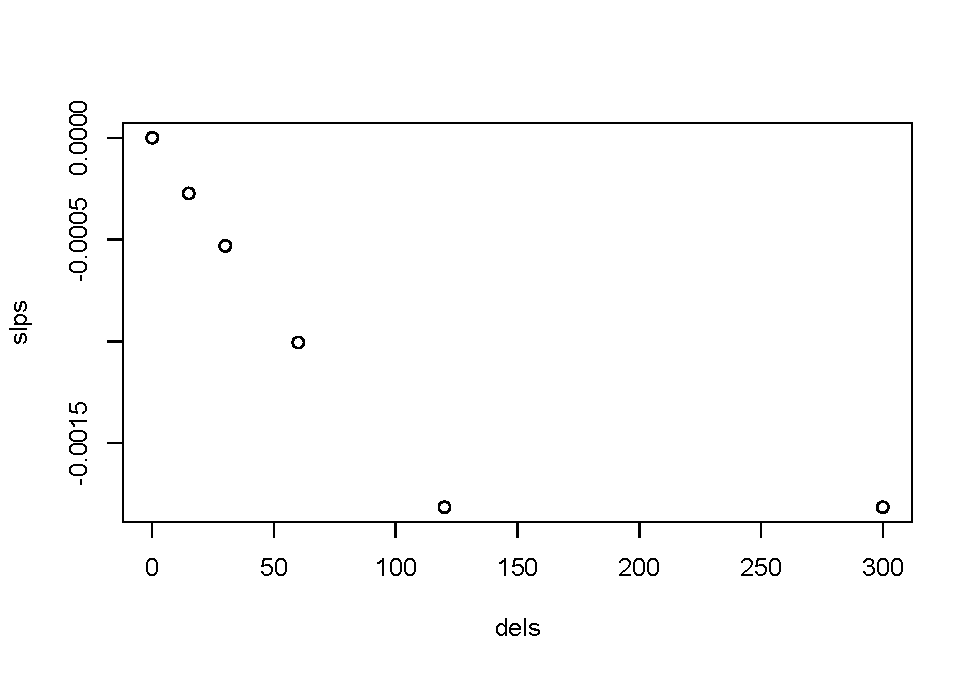
\includegraphics{bookdown_files/figure-latex/intslps-1.pdf}
\caption{\label{fig:intslps}基于 Ci 的不同延时下的斜率变化}
\end{figure}

\begin{Shaded}
\begin{Highlighting}[]
\KeywordTok{summary}\NormalTok{(}\KeywordTok{lm}\NormalTok{(slps }\OperatorTok{~}\StringTok{ }\NormalTok{dels }\OperatorTok{-}\StringTok{ }\DecValTok{1}\NormalTok{))}
\end{Highlighting}
\end{Shaded}

\begin{verbatim}
## 
## Call:
## lm(formula = slps ~ dels - 1)
## 
## Residuals:
##                   dataCi15$Cifull  dataCi30$Cifull  dataCi60$Cifull 
##       -2.711e-19       -1.574e-04       -2.995e-04       -5.424e-04 
## dataCi120$Cifull dataCi300$Cifull 
##       -8.881e-04        5.015e-04 
## 
## Coefficients:
##       Estimate Std. Error t value Pr(>|t|)   
## dels -7.72e-06   1.63e-06  -4.738  0.00516 **
## ---
## Signif. codes:  0 '***' 0.001 '**' 0.01 '*' 0.05 '.' 0.1 ' ' 1
## 
## Residual standard error: 0.0005383 on 5 degrees of freedom
## Multiple R-squared:  0.8178, Adjusted R-squared:  0.7814 
## F-statistic: 22.44 on 1 and 5 DF,  p-value: 0.005161
\end{verbatim}

基于 Cc 的补偿点计算结果:

\begin{Shaded}
\begin{Highlighting}[]
\CommentTok{# 仅使用 Cc < 75的数据点拟合,过程同ci}
\NormalTok{dataCc <-}\StringTok{ }\NormalTok{data[data}\OperatorTok{$}\NormalTok{Ccfull }\OperatorTok{<}\StringTok{ }\DecValTok{75}\NormalTok{, ]}
\NormalTok{dataCc0 <-}\StringTok{ }\NormalTok{dataCc[dataCc}\OperatorTok{$}\NormalTok{Delay }\OperatorTok{==}\StringTok{ "0"}\NormalTok{, ]}
\NormalTok{dataCc15 <-}\StringTok{ }\NormalTok{dataCc[dataCc}\OperatorTok{$}\NormalTok{Delay }\OperatorTok{==}\StringTok{ "15"}\NormalTok{, ]}
\NormalTok{dataCc30 <-}\StringTok{ }\NormalTok{dataCc[dataCc}\OperatorTok{$}\NormalTok{Delay }\OperatorTok{==}\StringTok{ "30"}\NormalTok{, ]}
\NormalTok{dataCc60 <-}\StringTok{ }\NormalTok{dataCc[dataCc}\OperatorTok{$}\NormalTok{Delay }\OperatorTok{==}\StringTok{ "60"}\NormalTok{, ]}
\NormalTok{dataCc120 <-}\StringTok{ }\NormalTok{dataCc[dataCc}\OperatorTok{$}\NormalTok{Delay }\OperatorTok{==}\StringTok{ "120"}\NormalTok{, ]}
\NormalTok{dataCc300 <-}\StringTok{ }\NormalTok{dataCc[dataCc}\OperatorTok{$}\NormalTok{Delay }\OperatorTok{==}\StringTok{ "300"}\NormalTok{, ]}

\CommentTok{# 无延迟数据}
\NormalTok{m1 <-}\StringTok{ }\KeywordTok{lm}\NormalTok{(dataCc0}\OperatorTok{$}\NormalTok{Anet }\OperatorTok{~}\StringTok{ }\NormalTok{dataCc0}\OperatorTok{$}\NormalTok{Ccfull)}
\KeywordTok{summary}\NormalTok{(m1)}
\end{Highlighting}
\end{Shaded}

\begin{verbatim}
## 
## Call:
## lm(formula = dataCc0$Anet ~ dataCc0$Ccfull)
## 
## Residuals:
##       Min        1Q    Median        3Q       Max 
## -0.075648 -0.025444  0.009857  0.031706  0.039431 
## 
## Coefficients:
##                  Estimate Std. Error t value Pr(>|t|)    
## (Intercept)    -8.4062011  0.0181852  -462.3   <2e-16 ***
## dataCc0$Ccfull  0.1438710  0.0003527   407.9   <2e-16 ***
## ---
## Signif. codes:  0 '***' 0.001 '**' 0.01 '*' 0.05 '.' 0.1 ' ' 1
## 
## Residual standard error: 0.03599 on 48 degrees of freedom
## Multiple R-squared:  0.9997, Adjusted R-squared:  0.9997 
## F-statistic: 1.664e+05 on 1 and 48 DF,  p-value: < 2.2e-16
\end{verbatim}

\begin{Shaded}
\begin{Highlighting}[]
\NormalTok{Gamma0 <-}\StringTok{ }\OperatorTok{-}\NormalTok{m1}\OperatorTok{$}\NormalTok{coefficients[}\DecValTok{1}\NormalTok{] }\OperatorTok{/}\StringTok{ }\NormalTok{m1}\OperatorTok{$}\NormalTok{coefficients[}\DecValTok{2}\NormalTok{]}

\CommentTok{#延时15s数据}
\NormalTok{m2 <-}\StringTok{ }\KeywordTok{lm}\NormalTok{(dataCc15}\OperatorTok{$}\NormalTok{Anet }\OperatorTok{~}\StringTok{ }\NormalTok{dataCc15}\OperatorTok{$}\NormalTok{Ccfull)}
\KeywordTok{summary}\NormalTok{(m2)}
\end{Highlighting}
\end{Shaded}

\begin{verbatim}
## 
## Call:
## lm(formula = dataCc15$Anet ~ dataCc15$Ccfull)
## 
## Residuals:
##       Min        1Q    Median        3Q       Max 
## -0.075393 -0.025359  0.009824  0.031599  0.039299 
## 
## Coefficients:
##                   Estimate Std. Error t value Pr(>|t|)    
## (Intercept)     -8.2659145  0.0181243  -456.1   <2e-16 ***
## dataCc15$Ccfull  0.1435470  0.0003515   408.4   <2e-16 ***
## ---
## Signif. codes:  0 '***' 0.001 '**' 0.01 '*' 0.05 '.' 0.1 ' ' 1
## 
## Residual standard error: 0.03587 on 48 degrees of freedom
## Multiple R-squared:  0.9997, Adjusted R-squared:  0.9997 
## F-statistic: 1.668e+05 on 1 and 48 DF,  p-value: < 2.2e-16
\end{verbatim}

\begin{Shaded}
\begin{Highlighting}[]
\NormalTok{Gamma15 <-}\StringTok{ }\OperatorTok{-}\NormalTok{m2}\OperatorTok{$}\NormalTok{coefficients[}\DecValTok{1}\NormalTok{] }\OperatorTok{/}\StringTok{ }\NormalTok{m2}\OperatorTok{$}\NormalTok{coefficients[}\DecValTok{2}\NormalTok{]}

\CommentTok{#延时30s数据}
\NormalTok{m3 <-}\StringTok{ }\KeywordTok{lm}\NormalTok{(dataCc30}\OperatorTok{$}\NormalTok{Anet }\OperatorTok{~}\StringTok{ }\NormalTok{dataCc30}\OperatorTok{$}\NormalTok{Ccfull)}
\KeywordTok{summary}\NormalTok{(m3)}
\end{Highlighting}
\end{Shaded}

\begin{verbatim}
## 
## Call:
## lm(formula = dataCc30$Anet ~ dataCc30$Ccfull)
## 
## Residuals:
##       Min        1Q    Median        3Q       Max 
## -0.075158 -0.025280  0.009794  0.031501  0.039177 
## 
## Coefficients:
##                   Estimate Std. Error t value Pr(>|t|)    
## (Intercept)     -8.1312578  0.0180681  -450.0   <2e-16 ***
## dataCc30$Ccfull  0.1432414  0.0003504   408.8   <2e-16 ***
## ---
## Signif. codes:  0 '***' 0.001 '**' 0.01 '*' 0.05 '.' 0.1 ' ' 1
## 
## Residual standard error: 0.03576 on 48 degrees of freedom
## Multiple R-squared:  0.9997, Adjusted R-squared:  0.9997 
## F-statistic: 1.671e+05 on 1 and 48 DF,  p-value: < 2.2e-16
\end{verbatim}

\begin{Shaded}
\begin{Highlighting}[]
\NormalTok{Gamma30 <-}\StringTok{ }\OperatorTok{-}\NormalTok{m3}\OperatorTok{$}\NormalTok{coefficients[}\DecValTok{1}\NormalTok{] }\OperatorTok{/}\StringTok{ }\NormalTok{m3}\OperatorTok{$}\NormalTok{coefficients[}\DecValTok{2}\NormalTok{]}

\CommentTok{#延时60s数据}
\NormalTok{m4 <-}\StringTok{ }\KeywordTok{lm}\NormalTok{(dataCc60}\OperatorTok{$}\NormalTok{Anet }\OperatorTok{~}\StringTok{ }\NormalTok{dataCc60}\OperatorTok{$}\NormalTok{Ccfull)}
\KeywordTok{summary}\NormalTok{(m4)}
\end{Highlighting}
\end{Shaded}

\begin{verbatim}
## 
## Call:
## lm(formula = dataCc60$Anet ~ dataCc60$Ccfull)
## 
## Residuals:
##       Min        1Q    Median        3Q       Max 
## -0.074737 -0.025139  0.009739  0.031325  0.038959 
## 
## Coefficients:
##                   Estimate Std. Error t value Pr(>|t|)    
## (Intercept)     -7.8775340  0.0179675  -438.4   <2e-16 ***
## dataCc60$Ccfull  0.1426797  0.0003485   409.4   <2e-16 ***
## ---
## Signif. codes:  0 '***' 0.001 '**' 0.01 '*' 0.05 '.' 0.1 ' ' 1
## 
## Residual standard error: 0.03556 on 48 degrees of freedom
## Multiple R-squared:  0.9997, Adjusted R-squared:  0.9997 
## F-statistic: 1.676e+05 on 1 and 48 DF,  p-value: < 2.2e-16
\end{verbatim}

\begin{Shaded}
\begin{Highlighting}[]
\NormalTok{Gamma60 <-}\StringTok{ }\OperatorTok{-}\NormalTok{m4}\OperatorTok{$}\NormalTok{coefficients[}\DecValTok{1}\NormalTok{] }\OperatorTok{/}\StringTok{ }\NormalTok{m4}\OperatorTok{$}\NormalTok{coefficients[}\DecValTok{2}\NormalTok{]}

\CommentTok{#延时120s数据}
\NormalTok{m5 <-}\StringTok{ }\KeywordTok{lm}\NormalTok{(dataCc120}\OperatorTok{$}\NormalTok{Anet }\OperatorTok{~}\StringTok{ }\NormalTok{dataCc120}\OperatorTok{$}\NormalTok{Ccfull)}
\KeywordTok{summary}\NormalTok{(m5)}
\end{Highlighting}
\end{Shaded}

\begin{verbatim}
## 
## Call:
## lm(formula = dataCc120$Anet ~ dataCc120$Ccfull)
## 
## Residuals:
##       Min        1Q    Median        3Q       Max 
## -0.074060 -0.024912  0.009651  0.031042  0.038607 
## 
## Coefficients:
##                    Estimate Std. Error t value Pr(>|t|)    
## (Intercept)      -7.4246412  0.0178052  -417.0   <2e-16 ***
## dataCc120$Ccfull  0.1417238  0.0003453   410.4   <2e-16 ***
## ---
## Signif. codes:  0 '***' 0.001 '**' 0.01 '*' 0.05 '.' 0.1 ' ' 1
## 
## Residual standard error: 0.03524 on 48 degrees of freedom
## Multiple R-squared:  0.9997, Adjusted R-squared:  0.9997 
## F-statistic: 1.684e+05 on 1 and 48 DF,  p-value: < 2.2e-16
\end{verbatim}

\begin{Shaded}
\begin{Highlighting}[]
\NormalTok{Gamma120 <-}\StringTok{ }\OperatorTok{-}\NormalTok{m5}\OperatorTok{$}\NormalTok{coefficients[}\DecValTok{1}\NormalTok{] }\OperatorTok{/}\StringTok{ }\NormalTok{m5}\OperatorTok{$}\NormalTok{coefficients[}\DecValTok{2}\NormalTok{]}

\CommentTok{#延时300s数据}
\NormalTok{m6 <-}\StringTok{ }\KeywordTok{lm}\NormalTok{(dataCc300}\OperatorTok{$}\NormalTok{Anet }\OperatorTok{~}\StringTok{ }\NormalTok{dataCc300}\OperatorTok{$}\NormalTok{Ccfull)}
\KeywordTok{summary}\NormalTok{(m6)}
\end{Highlighting}
\end{Shaded}

\begin{verbatim}
## 
## Call:
## lm(formula = dataCc300$Anet ~ dataCc300$Ccfull)
## 
## Residuals:
##       Min        1Q    Median        3Q       Max 
## -0.074060 -0.024912  0.009651  0.031042  0.038607 
## 
## Coefficients:
##                    Estimate Std. Error t value Pr(>|t|)    
## (Intercept)      -7.4246412  0.0178052  -417.0   <2e-16 ***
## dataCc300$Ccfull  0.1417238  0.0003453   410.4   <2e-16 ***
## ---
## Signif. codes:  0 '***' 0.001 '**' 0.01 '*' 0.05 '.' 0.1 ' ' 1
## 
## Residual standard error: 0.03524 on 48 degrees of freedom
## Multiple R-squared:  0.9997, Adjusted R-squared:  0.9997 
## F-statistic: 1.684e+05 on 1 and 48 DF,  p-value: < 2.2e-16
\end{verbatim}

\begin{Shaded}
\begin{Highlighting}[]
\NormalTok{Gamma300 <-}\StringTok{ }\OperatorTok{-}\NormalTok{m6}\OperatorTok{$}\NormalTok{coefficients[}\DecValTok{1}\NormalTok{] }\OperatorTok{/}\StringTok{ }\NormalTok{m6}\OperatorTok{$}\NormalTok{coefficients[}\DecValTok{2}\NormalTok{]}
\end{Highlighting}
\end{Shaded}

\begin{Shaded}
\begin{Highlighting}[]
\NormalTok{GammaCc <-}\StringTok{ }\KeywordTok{c}\NormalTok{(Gamma0, Gamma15, Gamma30, Gamma60, Gamma120, Gamma300)}

\NormalTok{ints <-}
\StringTok{  }\KeywordTok{c}\NormalTok{(}
\NormalTok{    m1}\OperatorTok{$}\NormalTok{coefficients[}\DecValTok{1}\NormalTok{],}
\NormalTok{    m2}\OperatorTok{$}\NormalTok{coefficients[}\DecValTok{1}\NormalTok{],}
\NormalTok{    m3}\OperatorTok{$}\NormalTok{coefficients[}\DecValTok{1}\NormalTok{],}
\NormalTok{    m4}\OperatorTok{$}\NormalTok{coefficients[}\DecValTok{1}\NormalTok{],}
\NormalTok{    m5}\OperatorTok{$}\NormalTok{coefficients[}\DecValTok{1}\NormalTok{],}
\NormalTok{    m6}\OperatorTok{$}\NormalTok{coefficients[}\DecValTok{1}\NormalTok{]}
\NormalTok{  )}
\NormalTok{dels <-}\StringTok{ }\KeywordTok{c}\NormalTok{(}\DecValTok{0}\NormalTok{, }\DecValTok{15}\NormalTok{, }\DecValTok{30}\NormalTok{, }\DecValTok{60}\NormalTok{, }\DecValTok{120}\NormalTok{, }\DecValTok{300}\NormalTok{)}
\KeywordTok{plot}\NormalTok{(ints }\OperatorTok{~}\StringTok{ }\NormalTok{dels)}
\end{Highlighting}
\end{Shaded}

\begin{figure}
\centering
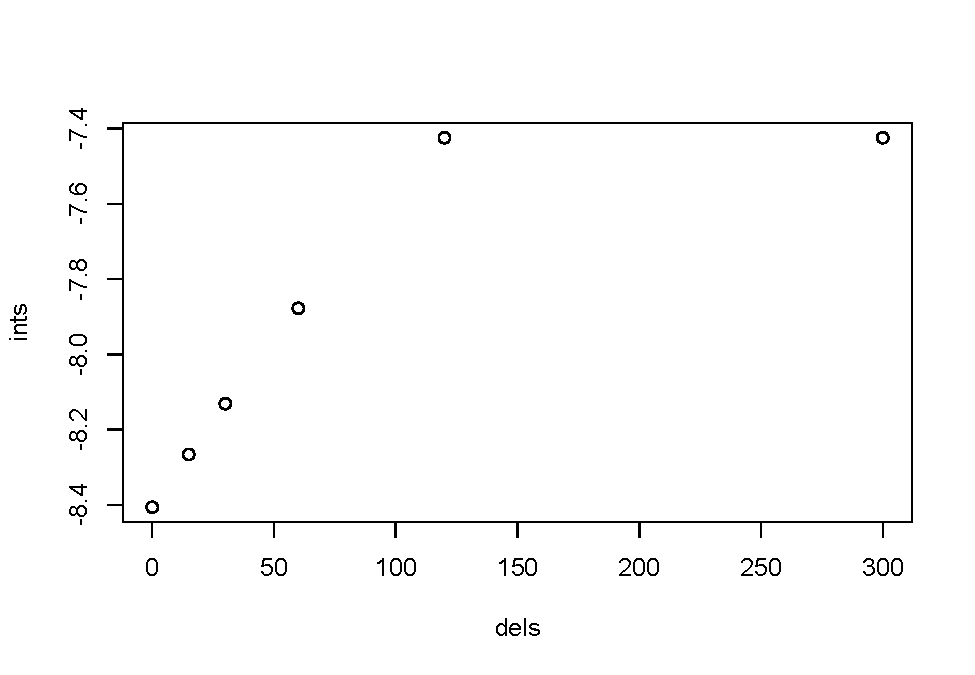
\includegraphics{bookdown_files/figure-latex/intdelaycc-1.pdf}
\caption{\label{fig:intdelaycc}基于 Cc 的不同延时下的时间}
\end{figure}

\begin{Shaded}
\begin{Highlighting}[]
\KeywordTok{summary}\NormalTok{(}\KeywordTok{lm}\NormalTok{(ints }\OperatorTok{~}\StringTok{ }\NormalTok{dels))}
\end{Highlighting}
\end{Shaded}

\begin{verbatim}
## 
## Call:
## lm(formula = ints ~ dels)
## 
## Residuals:
##   (Intercept) (Intercept).1 (Intercept).2 (Intercept).3 (Intercept).4 
##      -0.20760      -0.11478      -0.02759       0.13119       0.39421 
## (Intercept).5 
##      -0.17542 
## 
## Coefficients:
##              Estimate Std. Error t value Pr(>|t|)    
## (Intercept) -8.198602   0.136891 -59.891 4.65e-07 ***
## dels         0.003165   0.001015   3.118   0.0356 *  
## ---
## Signif. codes:  0 '***' 0.001 '**' 0.01 '*' 0.05 '.' 0.1 ' ' 1
## 
## Residual standard error: 0.2552 on 4 degrees of freedom
## Multiple R-squared:  0.7085, Adjusted R-squared:  0.6356 
## F-statistic:  9.72 on 1 and 4 DF,  p-value: 0.03561
\end{verbatim}

\begin{Shaded}
\begin{Highlighting}[]
\CommentTok{#GammaStar}
\CommentTok{# For Ci-based estimates, only use Ci < 100}
\NormalTok{dataCi <-}\StringTok{ }\NormalTok{data[data}\OperatorTok{$}\NormalTok{Cifull }\OperatorTok{<}\StringTok{ }\DecValTok{100}\NormalTok{,]}
\NormalTok{dataCi0 <-}\StringTok{ }\NormalTok{dataCi[dataCi}\OperatorTok{$}\NormalTok{Delay }\OperatorTok{==}\StringTok{ "0"}\NormalTok{,]}
\NormalTok{dataCi15 <-}\StringTok{ }\NormalTok{dataCi[dataCi}\OperatorTok{$}\NormalTok{Delay }\OperatorTok{==}\StringTok{ "15"}\NormalTok{,]}
\NormalTok{dataCi30 <-}\StringTok{ }\NormalTok{dataCi[dataCi}\OperatorTok{$}\NormalTok{Delay }\OperatorTok{==}\StringTok{ "30"}\NormalTok{,]}
\NormalTok{dataCi60 <-}\StringTok{ }\NormalTok{dataCi[dataCi}\OperatorTok{$}\NormalTok{Delay }\OperatorTok{==}\StringTok{ "60"}\NormalTok{,]}
\NormalTok{dataCi120 <-}\StringTok{ }\NormalTok{dataCi[dataCi}\OperatorTok{$}\NormalTok{Delay }\OperatorTok{==}\StringTok{ "120"}\NormalTok{,]}
\NormalTok{dataCi300 <-}\StringTok{ }\NormalTok{dataCi[dataCi}\OperatorTok{$}\NormalTok{Delay }\OperatorTok{==}\StringTok{ "300"}\NormalTok{,]}
\NormalTok{m1 <-}\StringTok{ }\KeywordTok{lm}\NormalTok{(dataCi0}\OperatorTok{$}\NormalTok{Aapp }\OperatorTok{~}\StringTok{ }\NormalTok{dataCi0}\OperatorTok{$}\NormalTok{Cifull)}
\KeywordTok{summary}\NormalTok{(m1)}
\end{Highlighting}
\end{Shaded}

\begin{verbatim}
## 
## Call:
## lm(formula = dataCi0$Aapp ~ dataCi0$Cifull)
## 
## Residuals:
##      Min       1Q   Median       3Q      Max 
## -0.13165 -0.04518  0.01711  0.05408  0.06699 
## 
## Coefficients:
##                  Estimate Std. Error t value Pr(>|t|)    
## (Intercept)    -5.2248105  0.0199353  -262.1   <2e-16 ***
## dataCi0$Cifull  0.1228632  0.0003089   397.8   <2e-16 ***
## ---
## Signif. codes:  0 '***' 0.001 '**' 0.01 '*' 0.05 '.' 0.1 ' ' 1
## 
## Residual standard error: 0.06081 on 69 degrees of freedom
## Multiple R-squared:  0.9996, Adjusted R-squared:  0.9996 
## F-statistic: 1.582e+05 on 1 and 69 DF,  p-value: < 2.2e-16
\end{verbatim}

\begin{Shaded}
\begin{Highlighting}[]
\NormalTok{Gamma0 <-}\StringTok{ }\OperatorTok{-}\NormalTok{m1}\OperatorTok{$}\NormalTok{coefficients[}\DecValTok{1}\NormalTok{] }\OperatorTok{/}\StringTok{ }\NormalTok{m1}\OperatorTok{$}\NormalTok{coefficients[}\DecValTok{2}\NormalTok{]}
\NormalTok{m2 <-}\StringTok{ }\KeywordTok{lm}\NormalTok{(dataCi15}\OperatorTok{$}\NormalTok{Aapp }\OperatorTok{~}\StringTok{ }\NormalTok{dataCi15}\OperatorTok{$}\NormalTok{Cifull)}
\KeywordTok{summary}\NormalTok{(m2)}
\end{Highlighting}
\end{Shaded}

\begin{verbatim}
## 
## Call:
## lm(formula = dataCi15$Aapp ~ dataCi15$Cifull)
## 
## Residuals:
##      Min       1Q   Median       3Q      Max 
## -0.13119 -0.04502  0.01705  0.05389  0.06676 
## 
## Coefficients:
##                   Estimate Std. Error t value Pr(>|t|)    
## (Intercept)     -5.0873326  0.0198665  -256.1   <2e-16 ***
## dataCi15$Cifull  0.1225900  0.0003078   398.3   <2e-16 ***
## ---
## Signif. codes:  0 '***' 0.001 '**' 0.01 '*' 0.05 '.' 0.1 ' ' 1
## 
## Residual standard error: 0.0606 on 69 degrees of freedom
## Multiple R-squared:  0.9996, Adjusted R-squared:  0.9996 
## F-statistic: 1.586e+05 on 1 and 69 DF,  p-value: < 2.2e-16
\end{verbatim}

\begin{Shaded}
\begin{Highlighting}[]
\NormalTok{Gamma15 <-}\StringTok{ }\OperatorTok{-}\NormalTok{m2}\OperatorTok{$}\NormalTok{coefficients[}\DecValTok{1}\NormalTok{] }\OperatorTok{/}\StringTok{ }\NormalTok{m2}\OperatorTok{$}\NormalTok{coefficients[}\DecValTok{2}\NormalTok{]}
\NormalTok{m3 <-}\StringTok{ }\KeywordTok{lm}\NormalTok{(dataCi30}\OperatorTok{$}\NormalTok{Aapp }\OperatorTok{~}\StringTok{ }\NormalTok{dataCi30}\OperatorTok{$}\NormalTok{Cifull)}
\KeywordTok{summary}\NormalTok{(m3)}
\end{Highlighting}
\end{Shaded}

\begin{verbatim}
## 
## Call:
## lm(formula = dataCi30$Aapp ~ dataCi30$Cifull)
## 
## Residuals:
##      Min       1Q   Median       3Q      Max 
## -0.13076 -0.04488  0.01699  0.05372  0.06654 
## 
## Coefficients:
##                   Estimate Std. Error t value Pr(>|t|)    
## (Intercept)     -4.9553180  0.0198028  -250.2   <2e-16 ***
## dataCi30$Cifull  0.1223321  0.0003068   398.7   <2e-16 ***
## ---
## Signif. codes:  0 '***' 0.001 '**' 0.01 '*' 0.05 '.' 0.1 ' ' 1
## 
## Residual standard error: 0.0604 on 69 degrees of freedom
## Multiple R-squared:  0.9996, Adjusted R-squared:  0.9996 
## F-statistic: 1.59e+05 on 1 and 69 DF,  p-value: < 2.2e-16
\end{verbatim}

\begin{Shaded}
\begin{Highlighting}[]
\NormalTok{Gamma30 <-}\StringTok{ }\OperatorTok{-}\NormalTok{m3}\OperatorTok{$}\NormalTok{coefficients[}\DecValTok{1}\NormalTok{] }\OperatorTok{/}\StringTok{ }\NormalTok{m3}\OperatorTok{$}\NormalTok{coefficients[}\DecValTok{2}\NormalTok{]}
\NormalTok{m4 <-}\StringTok{ }\KeywordTok{lm}\NormalTok{(dataCi60}\OperatorTok{$}\NormalTok{Aapp }\OperatorTok{~}\StringTok{ }\NormalTok{dataCi60}\OperatorTok{$}\NormalTok{Cifull)}
\KeywordTok{summary}\NormalTok{(m4)}
\end{Highlighting}
\end{Shaded}

\begin{verbatim}
## 
## Call:
## lm(formula = dataCi60$Aapp ~ dataCi60$Cifull)
## 
## Residuals:
##      Min       1Q   Median       3Q      Max 
## -0.13001 -0.04462  0.01690  0.05341  0.06616 
## 
## Coefficients:
##                  Estimate Std. Error t value Pr(>|t|)    
## (Intercept)     -4.706429   0.019689  -239.0   <2e-16 ***
## dataCi60$Cifull  0.121858   0.000305   399.5   <2e-16 ***
## ---
## Signif. codes:  0 '***' 0.001 '**' 0.01 '*' 0.05 '.' 0.1 ' ' 1
## 
## Residual standard error: 0.06006 on 69 degrees of freedom
## Multiple R-squared:  0.9996, Adjusted R-squared:  0.9996 
## F-statistic: 1.596e+05 on 1 and 69 DF,  p-value: < 2.2e-16
\end{verbatim}

\begin{Shaded}
\begin{Highlighting}[]
\NormalTok{Gamma60 <-}\StringTok{ }\OperatorTok{-}\NormalTok{m4}\OperatorTok{$}\NormalTok{coefficients[}\DecValTok{1}\NormalTok{] }\OperatorTok{/}\StringTok{ }\NormalTok{m4}\OperatorTok{$}\NormalTok{coefficients[}\DecValTok{2}\NormalTok{]}
\NormalTok{m5 <-}\StringTok{ }\KeywordTok{lm}\NormalTok{(dataCi120}\OperatorTok{$}\NormalTok{Aapp }\OperatorTok{~}\StringTok{ }\NormalTok{dataCi120}\OperatorTok{$}\NormalTok{Cifull)}
\KeywordTok{summary}\NormalTok{(m5)}
\end{Highlighting}
\end{Shaded}

\begin{verbatim}
## 
## Call:
## lm(formula = dataCi120$Aapp ~ dataCi120$Cifull)
## 
## Residuals:
##      Min       1Q   Median       3Q      Max 
## -0.12879 -0.04421  0.01673  0.05292  0.06555 
## 
## Coefficients:
##                    Estimate Std. Error t value Pr(>|t|)    
## (Intercept)      -4.2616980  0.0195062  -218.5   <2e-16 ***
## dataCi120$Cifull  0.1210486  0.0003022   400.5   <2e-16 ***
## ---
## Signif. codes:  0 '***' 0.001 '**' 0.01 '*' 0.05 '.' 0.1 ' ' 1
## 
## Residual standard error: 0.0595 on 69 degrees of freedom
## Multiple R-squared:  0.9996, Adjusted R-squared:  0.9996 
## F-statistic: 1.604e+05 on 1 and 69 DF,  p-value: < 2.2e-16
\end{verbatim}

\begin{Shaded}
\begin{Highlighting}[]
\NormalTok{Gamma120 <-}\StringTok{ }\OperatorTok{-}\NormalTok{m5}\OperatorTok{$}\NormalTok{coefficients[}\DecValTok{1}\NormalTok{] }\OperatorTok{/}\StringTok{ }\NormalTok{m5}\OperatorTok{$}\NormalTok{coefficients[}\DecValTok{2}\NormalTok{]}
\NormalTok{m6 <-}\StringTok{ }\KeywordTok{lm}\NormalTok{(dataCi300}\OperatorTok{$}\NormalTok{Aapp }\OperatorTok{~}\StringTok{ }\NormalTok{dataCi300}\OperatorTok{$}\NormalTok{Cifull)}
\KeywordTok{summary}\NormalTok{(m6)}
\end{Highlighting}
\end{Shaded}

\begin{verbatim}
## 
## Call:
## lm(formula = dataCi300$Aapp ~ dataCi300$Cifull)
## 
## Residuals:
##      Min       1Q   Median       3Q      Max 
## -0.12662 -0.04346  0.01645  0.05202  0.06444 
## 
## Coefficients:
##                    Estimate Std. Error t value Pr(>|t|)    
## (Intercept)      -3.2402030  0.0191773  -169.0   <2e-16 ***
## dataCi300$Cifull  0.1193852  0.0002971   401.8   <2e-16 ***
## ---
## Signif. codes:  0 '***' 0.001 '**' 0.01 '*' 0.05 '.' 0.1 ' ' 1
## 
## Residual standard error: 0.05849 on 69 degrees of freedom
## Multiple R-squared:  0.9996, Adjusted R-squared:  0.9996 
## F-statistic: 1.615e+05 on 1 and 69 DF,  p-value: < 2.2e-16
\end{verbatim}

\begin{Shaded}
\begin{Highlighting}[]
\NormalTok{Gamma300 <-}\StringTok{ }\OperatorTok{-}\NormalTok{m6}\OperatorTok{$}\NormalTok{coefficients[}\DecValTok{1}\NormalTok{] }\OperatorTok{/}\StringTok{ }\NormalTok{m6}\OperatorTok{$}\NormalTok{coefficients[}\DecValTok{2}\NormalTok{]}

\NormalTok{GammastarCi <-}
\StringTok{  }\KeywordTok{c}\NormalTok{(Gamma0, Gamma15, Gamma30, Gamma60, Gamma120, Gamma300)}

\CommentTok{# For Cc-based estimates, only use Cc < 75}
\NormalTok{dataCc <-}\StringTok{ }\NormalTok{data[data}\OperatorTok{$}\NormalTok{Ccfull }\OperatorTok{<}\StringTok{ }\DecValTok{75}\NormalTok{,]}
\NormalTok{dataCc0 <-}\StringTok{ }\NormalTok{dataCc[dataCc}\OperatorTok{$}\NormalTok{Delay }\OperatorTok{==}\StringTok{ "0"}\NormalTok{,]}
\NormalTok{dataCc15 <-}\StringTok{ }\NormalTok{dataCc[dataCc}\OperatorTok{$}\NormalTok{Delay }\OperatorTok{==}\StringTok{ "15"}\NormalTok{,]}
\NormalTok{dataCc30 <-}\StringTok{ }\NormalTok{dataCc[dataCc}\OperatorTok{$}\NormalTok{Delay }\OperatorTok{==}\StringTok{ "30"}\NormalTok{,]}
\NormalTok{dataCc60 <-}\StringTok{ }\NormalTok{dataCc[dataCc}\OperatorTok{$}\NormalTok{Delay }\OperatorTok{==}\StringTok{ "60"}\NormalTok{,]}
\NormalTok{dataCc120 <-}\StringTok{ }\NormalTok{dataCc[dataCc}\OperatorTok{$}\NormalTok{Delay }\OperatorTok{==}\StringTok{ "120"}\NormalTok{,]}
\NormalTok{dataCc300 <-}\StringTok{ }\NormalTok{dataCc[dataCc}\OperatorTok{$}\NormalTok{Delay }\OperatorTok{==}\StringTok{ "300"}\NormalTok{,]}
\NormalTok{m1 <-}\StringTok{ }\KeywordTok{lm}\NormalTok{(dataCc0}\OperatorTok{$}\NormalTok{Aapp }\OperatorTok{~}\StringTok{ }\NormalTok{dataCc0}\OperatorTok{$}\NormalTok{Ccfull)}
\KeywordTok{summary}\NormalTok{(m1)}
\end{Highlighting}
\end{Shaded}

\begin{verbatim}
## 
## Call:
## lm(formula = dataCc0$Aapp ~ dataCc0$Ccfull)
## 
## Residuals:
##       Min        1Q    Median        3Q       Max 
## -0.075648 -0.025444  0.009857  0.031706  0.039431 
## 
## Coefficients:
##                  Estimate Std. Error t value Pr(>|t|)    
## (Intercept)    -6.4062011  0.0181852  -352.3   <2e-16 ***
## dataCc0$Ccfull  0.1438710  0.0003527   407.9   <2e-16 ***
## ---
## Signif. codes:  0 '***' 0.001 '**' 0.01 '*' 0.05 '.' 0.1 ' ' 1
## 
## Residual standard error: 0.03599 on 48 degrees of freedom
## Multiple R-squared:  0.9997, Adjusted R-squared:  0.9997 
## F-statistic: 1.664e+05 on 1 and 48 DF,  p-value: < 2.2e-16
\end{verbatim}

\begin{Shaded}
\begin{Highlighting}[]
\NormalTok{Gamma0 <-}\StringTok{ }\OperatorTok{-}\NormalTok{m1}\OperatorTok{$}\NormalTok{coefficients[}\DecValTok{1}\NormalTok{] }\OperatorTok{/}\StringTok{ }\NormalTok{m1}\OperatorTok{$}\NormalTok{coefficients[}\DecValTok{2}\NormalTok{]}
\NormalTok{m2 <-}\StringTok{ }\KeywordTok{lm}\NormalTok{(dataCc15}\OperatorTok{$}\NormalTok{Aapp }\OperatorTok{~}\StringTok{ }\NormalTok{dataCc15}\OperatorTok{$}\NormalTok{Ccfull)}
\KeywordTok{summary}\NormalTok{(m2)}
\end{Highlighting}
\end{Shaded}

\begin{verbatim}
## 
## Call:
## lm(formula = dataCc15$Aapp ~ dataCc15$Ccfull)
## 
## Residuals:
##       Min        1Q    Median        3Q       Max 
## -0.075393 -0.025359  0.009824  0.031599  0.039299 
## 
## Coefficients:
##                   Estimate Std. Error t value Pr(>|t|)    
## (Intercept)     -6.2659145  0.0181243  -345.7   <2e-16 ***
## dataCc15$Ccfull  0.1435470  0.0003515   408.4   <2e-16 ***
## ---
## Signif. codes:  0 '***' 0.001 '**' 0.01 '*' 0.05 '.' 0.1 ' ' 1
## 
## Residual standard error: 0.03587 on 48 degrees of freedom
## Multiple R-squared:  0.9997, Adjusted R-squared:  0.9997 
## F-statistic: 1.668e+05 on 1 and 48 DF,  p-value: < 2.2e-16
\end{verbatim}

\begin{Shaded}
\begin{Highlighting}[]
\NormalTok{Gamma15 <-}\StringTok{ }\OperatorTok{-}\NormalTok{m2}\OperatorTok{$}\NormalTok{coefficients[}\DecValTok{1}\NormalTok{] }\OperatorTok{/}\StringTok{ }\NormalTok{m2}\OperatorTok{$}\NormalTok{coefficients[}\DecValTok{2}\NormalTok{]}
\NormalTok{m3 <-}\StringTok{ }\KeywordTok{lm}\NormalTok{(dataCc30}\OperatorTok{$}\NormalTok{Aapp }\OperatorTok{~}\StringTok{ }\NormalTok{dataCc30}\OperatorTok{$}\NormalTok{Ccfull)}
\KeywordTok{summary}\NormalTok{(m3)}
\end{Highlighting}
\end{Shaded}

\begin{verbatim}
## 
## Call:
## lm(formula = dataCc30$Aapp ~ dataCc30$Ccfull)
## 
## Residuals:
##       Min        1Q    Median        3Q       Max 
## -0.075158 -0.025280  0.009794  0.031501  0.039177 
## 
## Coefficients:
##                   Estimate Std. Error t value Pr(>|t|)    
## (Intercept)     -6.1312578  0.0180681  -339.3   <2e-16 ***
## dataCc30$Ccfull  0.1432414  0.0003504   408.8   <2e-16 ***
## ---
## Signif. codes:  0 '***' 0.001 '**' 0.01 '*' 0.05 '.' 0.1 ' ' 1
## 
## Residual standard error: 0.03576 on 48 degrees of freedom
## Multiple R-squared:  0.9997, Adjusted R-squared:  0.9997 
## F-statistic: 1.671e+05 on 1 and 48 DF,  p-value: < 2.2e-16
\end{verbatim}

\begin{Shaded}
\begin{Highlighting}[]
\NormalTok{Gamma30 <-}\StringTok{ }\OperatorTok{-}\NormalTok{m3}\OperatorTok{$}\NormalTok{coefficients[}\DecValTok{1}\NormalTok{] }\OperatorTok{/}\StringTok{ }\NormalTok{m3}\OperatorTok{$}\NormalTok{coefficients[}\DecValTok{2}\NormalTok{]}
\NormalTok{m4 <-}\StringTok{ }\KeywordTok{lm}\NormalTok{(dataCc60}\OperatorTok{$}\NormalTok{Aapp }\OperatorTok{~}\StringTok{ }\NormalTok{dataCc60}\OperatorTok{$}\NormalTok{Ccfull)}
\KeywordTok{summary}\NormalTok{(m4)}
\end{Highlighting}
\end{Shaded}

\begin{verbatim}
## 
## Call:
## lm(formula = dataCc60$Aapp ~ dataCc60$Ccfull)
## 
## Residuals:
##       Min        1Q    Median        3Q       Max 
## -0.074737 -0.025139  0.009739  0.031325  0.038959 
## 
## Coefficients:
##                   Estimate Std. Error t value Pr(>|t|)    
## (Intercept)     -5.8775340  0.0179675  -327.1   <2e-16 ***
## dataCc60$Ccfull  0.1426797  0.0003485   409.4   <2e-16 ***
## ---
## Signif. codes:  0 '***' 0.001 '**' 0.01 '*' 0.05 '.' 0.1 ' ' 1
## 
## Residual standard error: 0.03556 on 48 degrees of freedom
## Multiple R-squared:  0.9997, Adjusted R-squared:  0.9997 
## F-statistic: 1.676e+05 on 1 and 48 DF,  p-value: < 2.2e-16
\end{verbatim}

\begin{Shaded}
\begin{Highlighting}[]
\NormalTok{Gamma60 <-}\StringTok{ }\OperatorTok{-}\NormalTok{m4}\OperatorTok{$}\NormalTok{coefficients[}\DecValTok{1}\NormalTok{] }\OperatorTok{/}\StringTok{ }\NormalTok{m4}\OperatorTok{$}\NormalTok{coefficients[}\DecValTok{2}\NormalTok{]}
\NormalTok{m5 <-}\StringTok{ }\KeywordTok{lm}\NormalTok{(dataCc120}\OperatorTok{$}\NormalTok{Aapp }\OperatorTok{~}\StringTok{ }\NormalTok{dataCc120}\OperatorTok{$}\NormalTok{Ccfull)}
\KeywordTok{summary}\NormalTok{(m5)}
\end{Highlighting}
\end{Shaded}

\begin{verbatim}
## 
## Call:
## lm(formula = dataCc120$Aapp ~ dataCc120$Ccfull)
## 
## Residuals:
##       Min        1Q    Median        3Q       Max 
## -0.074060 -0.024912  0.009651  0.031042  0.038607 
## 
## Coefficients:
##                    Estimate Std. Error t value Pr(>|t|)    
## (Intercept)      -5.4246412  0.0178052  -304.7   <2e-16 ***
## dataCc120$Ccfull  0.1417238  0.0003453   410.4   <2e-16 ***
## ---
## Signif. codes:  0 '***' 0.001 '**' 0.01 '*' 0.05 '.' 0.1 ' ' 1
## 
## Residual standard error: 0.03524 on 48 degrees of freedom
## Multiple R-squared:  0.9997, Adjusted R-squared:  0.9997 
## F-statistic: 1.684e+05 on 1 and 48 DF,  p-value: < 2.2e-16
\end{verbatim}

\begin{Shaded}
\begin{Highlighting}[]
\NormalTok{Gamma120 <-}\StringTok{ }\OperatorTok{-}\NormalTok{m5}\OperatorTok{$}\NormalTok{coefficients[}\DecValTok{1}\NormalTok{] }\OperatorTok{/}\StringTok{ }\NormalTok{m5}\OperatorTok{$}\NormalTok{coefficients[}\DecValTok{2}\NormalTok{]}
\NormalTok{m6 <-}\StringTok{ }\KeywordTok{lm}\NormalTok{(dataCc300}\OperatorTok{$}\NormalTok{Aapp }\OperatorTok{~}\StringTok{ }\NormalTok{dataCc300}\OperatorTok{$}\NormalTok{Ccfull)}
\KeywordTok{summary}\NormalTok{(m6)}
\end{Highlighting}
\end{Shaded}

\begin{verbatim}
## 
## Call:
## lm(formula = dataCc300$Aapp ~ dataCc300$Ccfull)
## 
## Residuals:
##       Min        1Q    Median        3Q       Max 
## -0.072835 -0.024500  0.009492  0.030529  0.037969 
## 
## Coefficients:
##                    Estimate Std. Error t value Pr(>|t|)    
## (Intercept)      -4.3867121  0.0175110  -250.5   <2e-16 ***
## dataCc300$Ccfull  0.1397661  0.0003396   411.5   <2e-16 ***
## ---
## Signif. codes:  0 '***' 0.001 '**' 0.01 '*' 0.05 '.' 0.1 ' ' 1
## 
## Residual standard error: 0.03466 on 48 degrees of freedom
## Multiple R-squared:  0.9997, Adjusted R-squared:  0.9997 
## F-statistic: 1.694e+05 on 1 and 48 DF,  p-value: < 2.2e-16
\end{verbatim}

\begin{Shaded}
\begin{Highlighting}[]
\NormalTok{Gamma300 <-}\StringTok{ }\OperatorTok{-}\NormalTok{m6}\OperatorTok{$}\NormalTok{coefficients[}\DecValTok{1}\NormalTok{] }\OperatorTok{/}\StringTok{ }\NormalTok{m6}\OperatorTok{$}\NormalTok{coefficients[}\DecValTok{2}\NormalTok{]}

\NormalTok{GammastarCc <-}
\StringTok{  }\KeywordTok{c}\NormalTok{(Gamma0, Gamma15, Gamma30, Gamma60, Gamma120, Gamma300)}

\NormalTok{Delay2 <-}\StringTok{ }\KeywordTok{c}\NormalTok{(}\StringTok{"0"}\NormalTok{, }\StringTok{"15"}\NormalTok{, }\StringTok{"30"}\NormalTok{, }\StringTok{"60"}\NormalTok{, }\StringTok{"120"}\NormalTok{, }\StringTok{"300"}\NormalTok{)}
\NormalTok{PRcomps <-}
\StringTok{  }\KeywordTok{as.data.frame}\NormalTok{(}\KeywordTok{cbind}\NormalTok{(Delay2, GammaCc, GammaCi, GammastarCc, GammastarCi))}
\KeywordTok{write.csv}\NormalTok{(PRcomps, }\StringTok{"./data/PRcomps.csv"}\NormalTok{)}

\NormalTok{ints <-}
\StringTok{  }\KeywordTok{c}\NormalTok{(}
\NormalTok{    m1}\OperatorTok{$}\NormalTok{coefficients[}\DecValTok{1}\NormalTok{],}
\NormalTok{    m2}\OperatorTok{$}\NormalTok{coefficients[}\DecValTok{1}\NormalTok{],}
\NormalTok{    m3}\OperatorTok{$}\NormalTok{coefficients[}\DecValTok{1}\NormalTok{],}
\NormalTok{    m4}\OperatorTok{$}\NormalTok{coefficients[}\DecValTok{1}\NormalTok{],}
\NormalTok{    m5}\OperatorTok{$}\NormalTok{coefficients[}\DecValTok{1}\NormalTok{],}
\NormalTok{    m6}\OperatorTok{$}\NormalTok{coefficients[}\DecValTok{1}\NormalTok{]}
\NormalTok{  )}
\NormalTok{dels <-}\StringTok{ }\KeywordTok{c}\NormalTok{(}\DecValTok{0}\NormalTok{, }\DecValTok{15}\NormalTok{, }\DecValTok{30}\NormalTok{, }\DecValTok{60}\NormalTok{, }\DecValTok{120}\NormalTok{, }\DecValTok{300}\NormalTok{)}
\KeywordTok{summary}\NormalTok{(}\KeywordTok{lm}\NormalTok{(ints }\OperatorTok{~}\StringTok{ }\NormalTok{dels))}
\end{Highlighting}
\end{Shaded}

\begin{verbatim}
## 
## Call:
## lm(formula = ints ~ dels)
## 
## Residuals:
##   (Intercept) (Intercept).1 (Intercept).2 (Intercept).3 (Intercept).4 
##    -0.0751633    -0.0347043     0.0001247     0.0541933     0.1077758 
## (Intercept).5 
##    -0.0522262 
## 
## Coefficients:
##              Estimate Std. Error t value Pr(>|t|)    
## (Intercept) -6.331038   0.041673 -151.92 1.13e-08 ***
## dels         0.006655   0.000309   21.54 2.75e-05 ***
## ---
## Signif. codes:  0 '***' 0.001 '**' 0.01 '*' 0.05 '.' 0.1 ' ' 1
## 
## Residual standard error: 0.07768 on 4 degrees of freedom
## Multiple R-squared:  0.9915, Adjusted R-squared:  0.9893 
## F-statistic: 463.9 on 1 and 4 DF,  p-value: 2.749e-05
\end{verbatim}

\begin{Shaded}
\begin{Highlighting}[]
\KeywordTok{plot}\NormalTok{(ints }\OperatorTok{~}\StringTok{ }\NormalTok{dels)}
\end{Highlighting}
\end{Shaded}

\begin{figure}
\centering
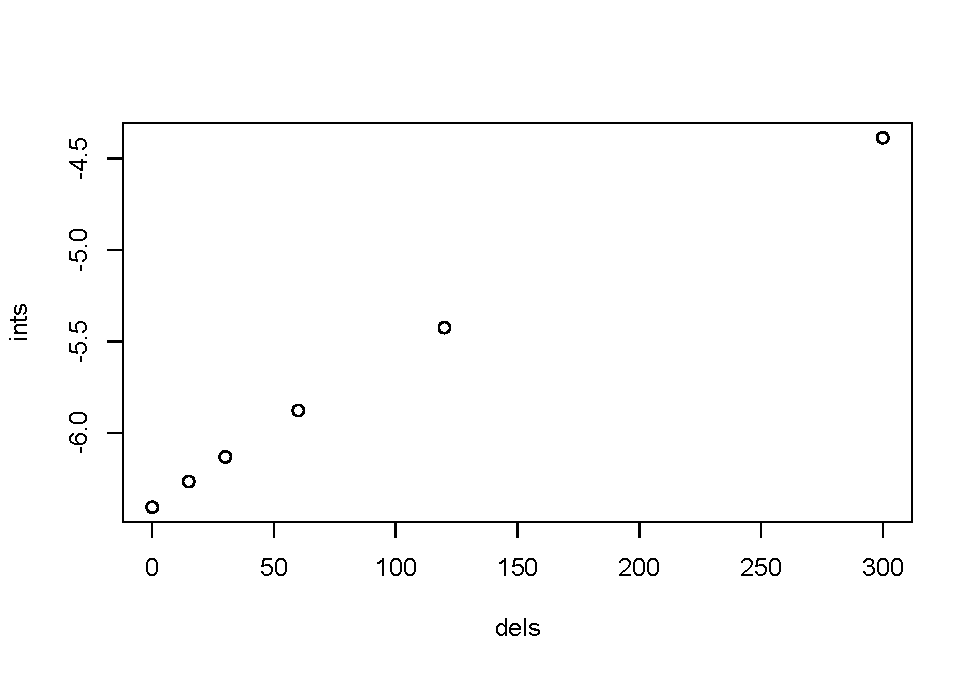
\includegraphics{bookdown_files/figure-latex/slpdelaycc-1.pdf}
\caption{\label{fig:slpdelaycc}基于 Cc 的不同延时下的截距}
\end{figure}

\hypertarget{no-phoresp-rubi}{%
\subsection{无光呼吸酶失活模块}\label{no-phoresp-rubi}}

该部分内容是在测量 ACi 曲线时检测 Rubisco 失活的影响 -- 从激活状态的变化导致了多少的偏移?

\hypertarget{data-pre}{%
\subsubsection{数据构造}\label{data-pre}}

基于文献,假定 \(CO_2\) 从 400 ppm 降低至 5 ppm 时,激活率从 100\% 降低至 80\%。

\begin{Shaded}
\begin{Highlighting}[]
\CommentTok{#Assume that Rubisco activation state drops from 100% at 400 ppm to 80% at 5 ppm Cr (line 273 is Cr of 400, Cc of 297; 5ppm Cr is 25 ppm Cc) roughly from Salvucci et al 1986, arabidopsis; assume linear response}

\CommentTok{#不同的cr对应了不同的cc浓度,}
\CommentTok{#此为cc的变化范围(cr从400降低至5)}
\NormalTok{ccslope <-}\StringTok{ }\KeywordTok{c}\NormalTok{(}\DecValTok{25}\NormalTok{, }\DecValTok{297}\NormalTok{)}
\CommentTok{#酶的激活率变化}
\NormalTok{raslope <-}\StringTok{ }\KeywordTok{c}\NormalTok{(}\FloatTok{0.80}\NormalTok{, }\FloatTok{1.00}\NormalTok{)}
\CommentTok{#得到cc变化对应rubisco激活率变化的关系}
\NormalTok{ram1 <-}\StringTok{ }\KeywordTok{lm}\NormalTok{(raslope }\OperatorTok{~}\StringTok{ }\NormalTok{ccslope)}
\NormalTok{raslope <-}\StringTok{ }\KeywordTok{coef}\NormalTok{(ram1)[}\DecValTok{2}\NormalTok{]}
\NormalTok{raint <-}\StringTok{ }\KeywordTok{coef}\NormalTok{(ram1)[}\DecValTok{1}\NormalTok{]}

\CommentTok{#根据公式计算酶部分失活后各个参数}
\NormalTok{vora1 <-}\StringTok{ }\NormalTok{(raslope }\OperatorTok{*}\StringTok{ }\NormalTok{Cc }\OperatorTok{+}\StringTok{ }\NormalTok{raint) }\OperatorTok{*}\StringTok{ }\NormalTok{Vomax }\OperatorTok{*}\StringTok{ }\NormalTok{O2 }\OperatorTok{/}\StringTok{ }\NormalTok{(O2 }\OperatorTok{+}\StringTok{ }\NormalTok{Ko }\OperatorTok{*}\StringTok{ }\NormalTok{(}\DecValTok{1} \OperatorTok{+}\StringTok{ }\NormalTok{Cc }\OperatorTok{/}\StringTok{ }\NormalTok{Kc))}
\NormalTok{vcra1 <-}\StringTok{ }\NormalTok{(raslope }\OperatorTok{*}\StringTok{ }\NormalTok{Cc }\OperatorTok{+}\StringTok{ }\NormalTok{raint) }\OperatorTok{*}\StringTok{ }\NormalTok{Vcmax }\OperatorTok{*}\StringTok{ }\NormalTok{(Cc) }\OperatorTok{/}\StringTok{ }\NormalTok{(Cc }\OperatorTok{+}\StringTok{ }\NormalTok{Kco)}
\NormalTok{Ara1 <-}\StringTok{ }\NormalTok{vcra1 }\OperatorTok{-}\StringTok{ }\FloatTok{0.5} \OperatorTok{*}\StringTok{ }\NormalTok{vora1 }\OperatorTok{-}\StringTok{ }\NormalTok{R}
\NormalTok{Aapparentra1 <-}\StringTok{ }\NormalTok{vcra1 }\OperatorTok{-}\StringTok{ }\FloatTok{0.5} \OperatorTok{*}\StringTok{ }\NormalTok{vora1}
\NormalTok{Cira1 <-}\StringTok{ }\NormalTok{Ara1 }\OperatorTok{/}\StringTok{ }\NormalTok{gm }\OperatorTok{+}\StringTok{ }\NormalTok{Cc}
\NormalTok{Cbra1 <-}\StringTok{ }\NormalTok{Ara1 }\OperatorTok{/}\StringTok{ }\NormalTok{gsw }\OperatorTok{+}\StringTok{ }\NormalTok{Cira1}
\NormalTok{Crra1 <-}\StringTok{ }\NormalTok{Ara1 }\OperatorTok{/}\StringTok{ }\NormalTok{BLC }\OperatorTok{+}\StringTok{ }\NormalTok{Cbra1}

\CommentTok{#失活后换算为分钟的变化斜率}
\NormalTok{Counter <-}\StringTok{ }\KeywordTok{as.numeric}\NormalTok{(}\KeywordTok{c}\NormalTok{(}\DecValTok{1}\OperatorTok{:}\KeywordTok{length}\NormalTok{(Cc)))}
\NormalTok{RateCr1model <-}\StringTok{ }\KeywordTok{lm}\NormalTok{(Crra1 }\OperatorTok{~}\StringTok{ }\NormalTok{Counter)}
\NormalTok{RateCr1 <-}\StringTok{ }\KeywordTok{coef}\NormalTok{(RateCr1model)[}\DecValTok{2}\NormalTok{] }\OperatorTok{*}\StringTok{ }\DecValTok{60}
\NormalTok{RateCb1model <-}\StringTok{ }\KeywordTok{lm}\NormalTok{(Cbra1 }\OperatorTok{~}\StringTok{ }\NormalTok{Counter)}
\NormalTok{RateCb1 <-}\StringTok{ }\KeywordTok{coef}\NormalTok{(RateCb1model)[}\DecValTok{2}\NormalTok{] }\OperatorTok{*}\StringTok{ }\DecValTok{60}
\NormalTok{RateCi1model <-}\StringTok{ }\KeywordTok{lm}\NormalTok{(Cira1 }\OperatorTok{~}\StringTok{ }\NormalTok{Counter)}
\NormalTok{RateCi1 <-}\StringTok{ }\KeywordTok{coef}\NormalTok{(RateCi1model)[}\DecValTok{2}\NormalTok{] }\OperatorTok{*}\StringTok{ }\DecValTok{60}
\NormalTok{RateCcmodel <-}\StringTok{ }\KeywordTok{lm}\NormalTok{(Cc }\OperatorTok{~}\StringTok{ }\NormalTok{Counter)}
\NormalTok{RateCc <-}\StringTok{ }\KeywordTok{coef}\NormalTok{(RateCcmodel)[}\DecValTok{2}\NormalTok{] }\OperatorTok{*}\StringTok{ }\DecValTok{60}

\CommentTok{#假定在5ppm时下降为40%}
\NormalTok{ccslope2 <-}\StringTok{ }\KeywordTok{c}\NormalTok{(}\DecValTok{25}\NormalTok{, }\DecValTok{297}\NormalTok{)}
\NormalTok{raslope2 <-}\StringTok{ }\KeywordTok{c}\NormalTok{(}\FloatTok{0.40}\NormalTok{, }\FloatTok{1.00}\NormalTok{)}
\NormalTok{ram2 <-}\StringTok{ }\KeywordTok{lm}\NormalTok{(raslope2 }\OperatorTok{~}\StringTok{ }\NormalTok{ccslope2)}
\NormalTok{raslope2 <-}\StringTok{ }\KeywordTok{coef}\NormalTok{(ram2)[}\DecValTok{2}\NormalTok{]}
\NormalTok{raint2 <-}\StringTok{ }\KeywordTok{coef}\NormalTok{(ram2)[}\DecValTok{1}\NormalTok{]}

\NormalTok{vora2 <-}
\StringTok{  }\NormalTok{(raslope2 }\OperatorTok{*}\StringTok{ }\NormalTok{Cc }\OperatorTok{+}\StringTok{ }\NormalTok{raint2) }\OperatorTok{*}\StringTok{ }\NormalTok{Vomax }\OperatorTok{*}\StringTok{ }\NormalTok{O2 }\OperatorTok{/}\StringTok{ }\NormalTok{(O2 }\OperatorTok{+}\StringTok{ }\NormalTok{Ko }\OperatorTok{*}\StringTok{ }\NormalTok{(}\DecValTok{1} \OperatorTok{+}\StringTok{ }\NormalTok{Cc }\OperatorTok{/}\StringTok{ }\NormalTok{Kc)) }
\NormalTok{vcra2 <-}\StringTok{ }\NormalTok{(raslope2 }\OperatorTok{*}\StringTok{ }\NormalTok{Cc }\OperatorTok{+}\StringTok{ }\NormalTok{raint2) }\OperatorTok{*}\StringTok{ }\NormalTok{Vcmax }\OperatorTok{*}\StringTok{ }\NormalTok{(Cc) }\OperatorTok{/}\StringTok{ }\NormalTok{(Cc }\OperatorTok{+}\StringTok{ }\NormalTok{Kco) }
\NormalTok{Ara2 <-}\StringTok{ }\NormalTok{vcra2 }\OperatorTok{-}\StringTok{ }\FloatTok{0.5} \OperatorTok{*}\StringTok{ }\NormalTok{vora2 }\OperatorTok{-}\StringTok{ }\NormalTok{R }
\NormalTok{Aapparentra2 <-}\StringTok{ }\NormalTok{vcra2 }\OperatorTok{-}\StringTok{ }\FloatTok{0.5} \OperatorTok{*}\StringTok{ }\NormalTok{vora2 }
\NormalTok{Cira2 <-}\StringTok{ }\NormalTok{Ara2 }\OperatorTok{/}\StringTok{ }\NormalTok{gm }\OperatorTok{+}\StringTok{ }\NormalTok{Cc }\CommentTok{#umol mol-1}
\NormalTok{Cbra2 <-}\StringTok{ }\NormalTok{Ara2 }\OperatorTok{/}\StringTok{ }\NormalTok{gsw }\OperatorTok{+}\StringTok{ }\NormalTok{Cira2 }\CommentTok{#umol mol-1}
\NormalTok{Crra2 <-}\StringTok{ }\NormalTok{Ara2 }\OperatorTok{/}\StringTok{ }\NormalTok{BLC }\OperatorTok{+}\StringTok{ }\NormalTok{Cbra2 }\CommentTok{#umol mol-1}
\NormalTok{Counter <-}\StringTok{ }\KeywordTok{as.numeric}\NormalTok{(}\KeywordTok{c}\NormalTok{(}\DecValTok{1}\OperatorTok{:}\KeywordTok{length}\NormalTok{(Cc)))}
\NormalTok{RateCr2model <-}\StringTok{ }\KeywordTok{lm}\NormalTok{(Crra2 }\OperatorTok{~}\StringTok{ }\NormalTok{Counter)}
\NormalTok{RateCr2 <-}\StringTok{ }\KeywordTok{coef}\NormalTok{(RateCr2model)[}\DecValTok{2}\NormalTok{] }\OperatorTok{*}\StringTok{ }\DecValTok{60} \CommentTok{#umol mol-1 min-1}
\NormalTok{RateCb2model <-}\StringTok{ }\KeywordTok{lm}\NormalTok{(Cbra2 }\OperatorTok{~}\StringTok{ }\NormalTok{Counter)}
\NormalTok{RateCb2 <-}\StringTok{ }\KeywordTok{coef}\NormalTok{(RateCb2model)[}\DecValTok{2}\NormalTok{] }\OperatorTok{*}\StringTok{ }\DecValTok{60} \CommentTok{#umol mol-1 min-1}
\NormalTok{RateCi2model <-}\StringTok{ }\KeywordTok{lm}\NormalTok{(Cira2 }\OperatorTok{~}\StringTok{ }\NormalTok{Counter)}
\NormalTok{RateCi2 <-}\StringTok{ }\KeywordTok{coef}\NormalTok{(RateCi2model)[}\DecValTok{2}\NormalTok{] }\OperatorTok{*}\StringTok{ }\DecValTok{60} \CommentTok{#umol mol-1 min-1}
\NormalTok{RateCcmodel <-}\StringTok{ }\KeywordTok{lm}\NormalTok{(Cc }\OperatorTok{~}\StringTok{ }\NormalTok{Counter)}
\NormalTok{RateCc <-}\StringTok{ }\KeywordTok{coef}\NormalTok{(RateCcmodel)[}\DecValTok{2}\NormalTok{] }\OperatorTok{*}\StringTok{ }\DecValTok{60} \CommentTok{#umol mol-1 min-1}

\CommentTok{#假定在5ppm时下降为20%}
\NormalTok{ccslope3 <-}\StringTok{ }\KeywordTok{c}\NormalTok{(}\DecValTok{25}\NormalTok{, }\DecValTok{297}\NormalTok{)}
\NormalTok{raslope3 <-}\StringTok{ }\KeywordTok{c}\NormalTok{(}\FloatTok{0.20}\NormalTok{, }\FloatTok{1.00}\NormalTok{)}
\NormalTok{ram3 <-}\StringTok{ }\KeywordTok{lm}\NormalTok{(raslope3 }\OperatorTok{~}\StringTok{ }\NormalTok{ccslope3)}
\NormalTok{raslope3 <-}\StringTok{ }\KeywordTok{coef}\NormalTok{(ram3)[}\DecValTok{2}\NormalTok{]}
\NormalTok{raint3 <-}\StringTok{ }\KeywordTok{coef}\NormalTok{(ram3)[}\DecValTok{1}\NormalTok{]}

\NormalTok{vora3 <-}
\StringTok{  }\NormalTok{(raslope3 }\OperatorTok{*}\StringTok{ }\NormalTok{Cc }\OperatorTok{+}\StringTok{ }\NormalTok{raint3) }\OperatorTok{*}\StringTok{ }\NormalTok{Vomax }\OperatorTok{*}\StringTok{ }\NormalTok{O2 }\OperatorTok{/}\StringTok{ }\NormalTok{(O2 }\OperatorTok{+}\StringTok{ }\NormalTok{Ko }\OperatorTok{*}\StringTok{ }\NormalTok{(}\DecValTok{1} \OperatorTok{+}\StringTok{ }\NormalTok{Cc }\OperatorTok{/}\StringTok{ }\NormalTok{Kc)) }
\NormalTok{vcra3 <-}\StringTok{ }\NormalTok{(raslope3 }\OperatorTok{*}\StringTok{ }\NormalTok{Cc }\OperatorTok{+}\StringTok{ }\NormalTok{raint3) }\OperatorTok{*}\StringTok{ }\NormalTok{Vcmax }\OperatorTok{*}\StringTok{ }\NormalTok{(Cc) }\OperatorTok{/}\StringTok{ }\NormalTok{(Cc }\OperatorTok{+}\StringTok{ }\NormalTok{Kco) }
\NormalTok{Ara3 <-}\StringTok{ }\NormalTok{vcra3 }\OperatorTok{-}\StringTok{ }\FloatTok{0.5} \OperatorTok{*}\StringTok{ }\NormalTok{vora3 }\OperatorTok{-}\StringTok{ }\NormalTok{R }
\NormalTok{Aapparentra3 <-}\StringTok{ }\NormalTok{vcra3 }\OperatorTok{-}\StringTok{ }\FloatTok{0.5} \OperatorTok{*}\StringTok{ }\NormalTok{vora3 }
\NormalTok{Cira3 <-}\StringTok{ }\NormalTok{Ara3 }\OperatorTok{/}\StringTok{ }\NormalTok{gm }\OperatorTok{+}\StringTok{ }\NormalTok{Cc }
\NormalTok{Cbra3 <-}\StringTok{ }\NormalTok{Ara3 }\OperatorTok{/}\StringTok{ }\NormalTok{gsw }\OperatorTok{+}\StringTok{ }\NormalTok{Cira3 }
\NormalTok{Crra3 <-}\StringTok{ }\NormalTok{Ara3 }\OperatorTok{/}\StringTok{ }\NormalTok{BLC }\OperatorTok{+}\StringTok{ }\NormalTok{Cbra3 }
\NormalTok{Counter <-}\StringTok{ }\KeywordTok{as.numeric}\NormalTok{(}\KeywordTok{c}\NormalTok{(}\DecValTok{1}\OperatorTok{:}\KeywordTok{length}\NormalTok{(Cc)))}
\NormalTok{RateCr3model <-}\StringTok{ }\KeywordTok{lm}\NormalTok{(Crra3 }\OperatorTok{~}\StringTok{ }\NormalTok{Counter)}
\NormalTok{RateCr3 <-}\StringTok{ }\KeywordTok{coef}\NormalTok{(RateCr3model)[}\DecValTok{2}\NormalTok{] }\OperatorTok{*}\StringTok{ }\DecValTok{60} 
\NormalTok{RateCb3model <-}\StringTok{ }\KeywordTok{lm}\NormalTok{(Cbra3 }\OperatorTok{~}\StringTok{ }\NormalTok{Counter)}
\NormalTok{RateCb3 <-}\StringTok{ }\KeywordTok{coef}\NormalTok{(RateCb3model)[}\DecValTok{2}\NormalTok{] }\OperatorTok{*}\StringTok{ }\DecValTok{60} 
\NormalTok{RateCi3model <-}\StringTok{ }\KeywordTok{lm}\NormalTok{(Cira3 }\OperatorTok{~}\StringTok{ }\NormalTok{Counter)}
\NormalTok{RateCi3 <-}\StringTok{ }\KeywordTok{coef}\NormalTok{(RateCi3model)[}\DecValTok{2}\NormalTok{] }\OperatorTok{*}\StringTok{ }\DecValTok{60} 
\NormalTok{RateCcmodel <-}\StringTok{ }\KeywordTok{lm}\NormalTok{(Cc }\OperatorTok{~}\StringTok{ }\NormalTok{Counter)}
\NormalTok{RateCc <-}\StringTok{ }\KeywordTok{coef}\NormalTok{(RateCcmodel)[}\DecValTok{2}\NormalTok{] }\OperatorTok{*}\StringTok{ }\DecValTok{60} 

\NormalTok{Anet <-}\StringTok{ }\KeywordTok{c}\NormalTok{(A, Ara1, Ara2, Ara3)}
\NormalTok{Aapp <-}\StringTok{ }\KeywordTok{c}\NormalTok{(Aapparent, Aapparentra1, Aapparentra2, Aapparentra3)}
\NormalTok{Ccfull <-}\StringTok{ }\KeywordTok{rep}\NormalTok{(Cc, }\DecValTok{4}\NormalTok{)}
\NormalTok{Cifull <-}\StringTok{ }\KeywordTok{c}\NormalTok{(Ci, Cira1, Cira2, Cira3)}
\NormalTok{Deactivation <-}
\StringTok{  }\KeywordTok{c}\NormalTok{(}
    \KeywordTok{rep}\NormalTok{(}\StringTok{"None"}\NormalTok{, }\KeywordTok{length}\NormalTok{(A)),}
    \KeywordTok{rep}\NormalTok{(}\StringTok{"Low"}\NormalTok{, }\KeywordTok{length}\NormalTok{(Ara1)),}
    \KeywordTok{rep}\NormalTok{(}\StringTok{"Medium"}\NormalTok{, }\KeywordTok{length}\NormalTok{(Ara2)),}
    \KeywordTok{rep}\NormalTok{(}\StringTok{"High"}\NormalTok{, }\KeywordTok{length}\NormalTok{(Ara3))}
\NormalTok{  )}
\NormalTok{RASdata <-}
\StringTok{  }\KeywordTok{as.data.frame}\NormalTok{(}\KeywordTok{cbind}\NormalTok{(Anet, Aapp, Ccfull, Cifull, Deactivation))}
\KeywordTok{write.csv}\NormalTok{(RASdata, }\StringTok{"./data/RASdata.csv"}\NormalTok{)}
\end{Highlighting}
\end{Shaded}

\hypertarget{Graphs-deac}{%
\subsection{酶失活作图}\label{Graphs-deac}}

\begin{Shaded}
\begin{Highlighting}[]
\NormalTok{data <-}\StringTok{ }\KeywordTok{read.csv}\NormalTok{(}\StringTok{"./data/RASdata.csv"}\NormalTok{)}
\NormalTok{data}\OperatorTok{$}\NormalTok{Ccfull <-}\StringTok{ }\KeywordTok{as.numeric}\NormalTok{(data}\OperatorTok{$}\NormalTok{Ccfull)}
\NormalTok{data}\OperatorTok{$}\NormalTok{Deactivation <-}\StringTok{ }\KeywordTok{as.factor}\NormalTok{(data}\OperatorTok{$}\NormalTok{Deactivation)}

\NormalTok{AnetCc <-}
\StringTok{  }\KeywordTok{ggplot}\NormalTok{(data, }\KeywordTok{aes}\NormalTok{(}\DataTypeTok{x =}\NormalTok{ Ccfull, }\DataTypeTok{y =}\NormalTok{ Anet, }\DataTypeTok{colour =}\NormalTok{ Deactivation)) }\OperatorTok{+}
\StringTok{  }\KeywordTok{geom_point}\NormalTok{() }\OperatorTok{+}
\StringTok{  }\KeywordTok{labs}\NormalTok{(}\DataTypeTok{x =} \KeywordTok{expression}\NormalTok{(C[c] }\OperatorTok{~}\StringTok{ "("} \OperatorTok{*}\StringTok{ }\NormalTok{mu }\OperatorTok{*}\StringTok{ }\NormalTok{mol }\OperatorTok{~}\StringTok{ }\NormalTok{mol }\OperatorTok{^}\StringTok{ }\NormalTok{\{}
    \DecValTok{-1}
\NormalTok{  \} }\OperatorTok{*}\StringTok{ ")"}\NormalTok{),}
  \DataTypeTok{y =} \KeywordTok{expression}\NormalTok{(A[net] }\OperatorTok{~}\StringTok{ "("} \OperatorTok{*}\StringTok{ }\NormalTok{mu }\OperatorTok{*}\StringTok{ }\NormalTok{mol }\OperatorTok{~}\StringTok{ }\NormalTok{m }\OperatorTok{^}\StringTok{ }\NormalTok{\{}
    \DecValTok{-2}
\NormalTok{  \} }\OperatorTok{~}\StringTok{ }\NormalTok{s }\OperatorTok{^}\StringTok{ }\NormalTok{\{}
    \DecValTok{-1}
\NormalTok{  \} }\OperatorTok{*}\StringTok{ ")"}\NormalTok{)) }\OperatorTok{+}
\StringTok{  }\KeywordTok{labs}\NormalTok{(}\DataTypeTok{colour =} \StringTok{'Deactivation'}\NormalTok{) }\OperatorTok{+}
\StringTok{  }\KeywordTok{scale_x_continuous}\NormalTok{(}\DataTypeTok{limits =} \KeywordTok{c}\NormalTok{(}\DecValTok{25}\NormalTok{, }\DecValTok{100}\NormalTok{),}
                     \DataTypeTok{breaks =} \KeywordTok{c}\NormalTok{(}\DecValTok{25}\NormalTok{, }\DecValTok{40}\NormalTok{, }\DecValTok{55}\NormalTok{, }\DecValTok{70}\NormalTok{, }\DecValTok{85}\NormalTok{, }\DecValTok{100}\NormalTok{)) }\OperatorTok{+}
\StringTok{  }\KeywordTok{scale_y_continuous}\NormalTok{(}\DataTypeTok{limits =} \KeywordTok{c}\NormalTok{(}\OperatorTok{-}\DecValTok{5}\NormalTok{, }\DecValTok{5}\NormalTok{)) }\OperatorTok{+}
\StringTok{  }\KeywordTok{scale_colour_brewer}\NormalTok{(}\DataTypeTok{palette =} \StringTok{'Spectral'}\NormalTok{) }\OperatorTok{+}
\StringTok{  }\KeywordTok{geom_hline}\NormalTok{(}\DataTypeTok{yintercept =} \DecValTok{0}\NormalTok{) }\OperatorTok{+}
\StringTok{  }\KeywordTok{theme_bw}\NormalTok{() }\OperatorTok{+}
\StringTok{  }\KeywordTok{theme}\NormalTok{(}\DataTypeTok{panel.grid.major =} \KeywordTok{element_blank}\NormalTok{(),}
        \DataTypeTok{panel.grid.minor =} \KeywordTok{element_blank}\NormalTok{())}
\NormalTok{AnetCc}
\end{Highlighting}
\end{Shaded}

\begin{figure}
\centering
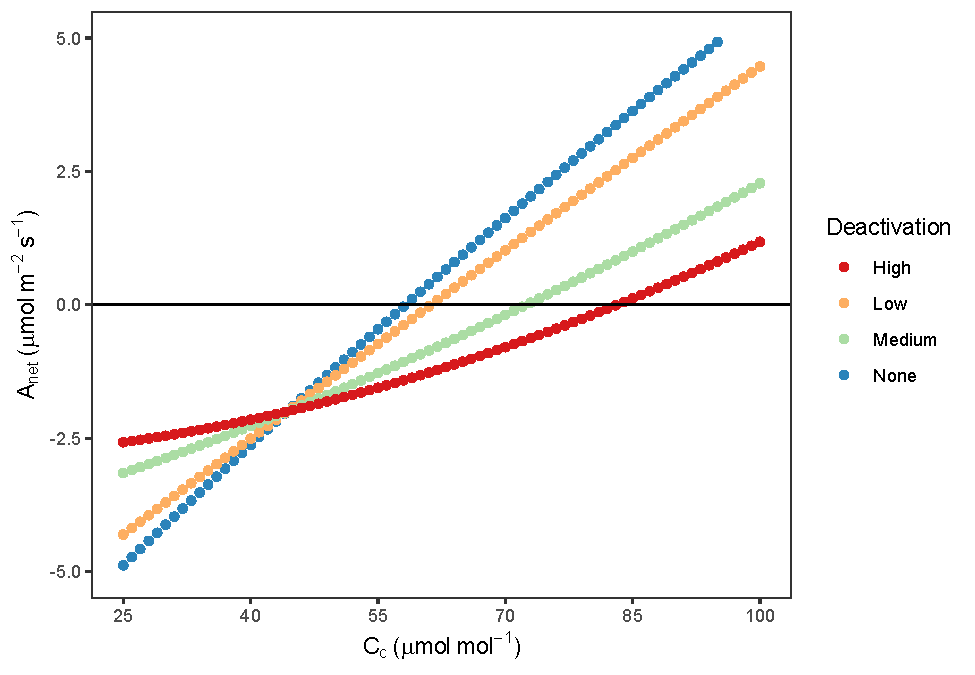
\includegraphics{bookdown_files/figure-latex/anetdeccc-1.pdf}
\caption{\label{fig:anetdeccc}Rubisco 不同失活程度时 Anet VS Cc}
\end{figure}

\begin{Shaded}
\begin{Highlighting}[]
\NormalTok{AnetCi <-}
\StringTok{  }\KeywordTok{ggplot}\NormalTok{(data, }\KeywordTok{aes}\NormalTok{(}\DataTypeTok{x =}\NormalTok{ Cifull, }\DataTypeTok{y =}\NormalTok{ Anet, }\DataTypeTok{colour =}\NormalTok{ Deactivation)) }\OperatorTok{+}
\StringTok{  }\KeywordTok{geom_point}\NormalTok{() }\OperatorTok{+}
\StringTok{  }\KeywordTok{labs}\NormalTok{(}\DataTypeTok{x =} \KeywordTok{expression}\NormalTok{(C[i] }\OperatorTok{~}\StringTok{ "("} \OperatorTok{*}\StringTok{ }\NormalTok{mu }\OperatorTok{*}\StringTok{ }\NormalTok{mol }\OperatorTok{~}\StringTok{ }\NormalTok{mol }\OperatorTok{^}\StringTok{ }\NormalTok{\{}
    \DecValTok{-1}
\NormalTok{  \} }\OperatorTok{*}\StringTok{ ")"}\NormalTok{),}
  \DataTypeTok{y =} \KeywordTok{expression}\NormalTok{(A[net] }\OperatorTok{~}\StringTok{ "("} \OperatorTok{*}\StringTok{ }\NormalTok{mu }\OperatorTok{*}\StringTok{ }\NormalTok{mol }\OperatorTok{~}\StringTok{ }\NormalTok{m }\OperatorTok{^}\StringTok{ }\NormalTok{\{}
    \DecValTok{-2}
\NormalTok{  \} }\OperatorTok{~}\StringTok{ }\NormalTok{s }\OperatorTok{^}\StringTok{ }\NormalTok{\{}
    \DecValTok{-1}
\NormalTok{  \} }\OperatorTok{*}\StringTok{ ")"}\NormalTok{)) }\OperatorTok{+}
\StringTok{  }\KeywordTok{labs}\NormalTok{(}\DataTypeTok{colour =} \StringTok{'Deactivation'}\NormalTok{) }\OperatorTok{+}
\StringTok{  }\KeywordTok{scale_x_continuous}\NormalTok{(}\DataTypeTok{limits =} \KeywordTok{c}\NormalTok{(}\DecValTok{25}\NormalTok{, }\DecValTok{100}\NormalTok{),}
                     \DataTypeTok{breaks =} \KeywordTok{c}\NormalTok{(}\DecValTok{25}\NormalTok{, }\DecValTok{40}\NormalTok{, }\DecValTok{55}\NormalTok{, }\DecValTok{70}\NormalTok{, }\DecValTok{85}\NormalTok{, }\DecValTok{100}\NormalTok{)) }\OperatorTok{+}
\StringTok{  }\KeywordTok{scale_y_continuous}\NormalTok{(}\DataTypeTok{limits =} \KeywordTok{c}\NormalTok{(}\OperatorTok{-}\DecValTok{5}\NormalTok{, }\DecValTok{5}\NormalTok{)) }\OperatorTok{+}
\StringTok{  }\KeywordTok{scale_colour_brewer}\NormalTok{(}\DataTypeTok{palette =} \StringTok{'Spectral'}\NormalTok{) }\OperatorTok{+}
\StringTok{  }\KeywordTok{geom_hline}\NormalTok{(}\DataTypeTok{yintercept =} \DecValTok{0}\NormalTok{) }\OperatorTok{+}
\StringTok{  }\KeywordTok{theme_bw}\NormalTok{() }\OperatorTok{+}
\StringTok{  }\KeywordTok{theme}\NormalTok{(}\DataTypeTok{panel.grid.major =} \KeywordTok{element_blank}\NormalTok{(),}
        \DataTypeTok{panel.grid.minor =} \KeywordTok{element_blank}\NormalTok{())}
\NormalTok{AnetCi}
\end{Highlighting}
\end{Shaded}

\begin{figure}
\centering
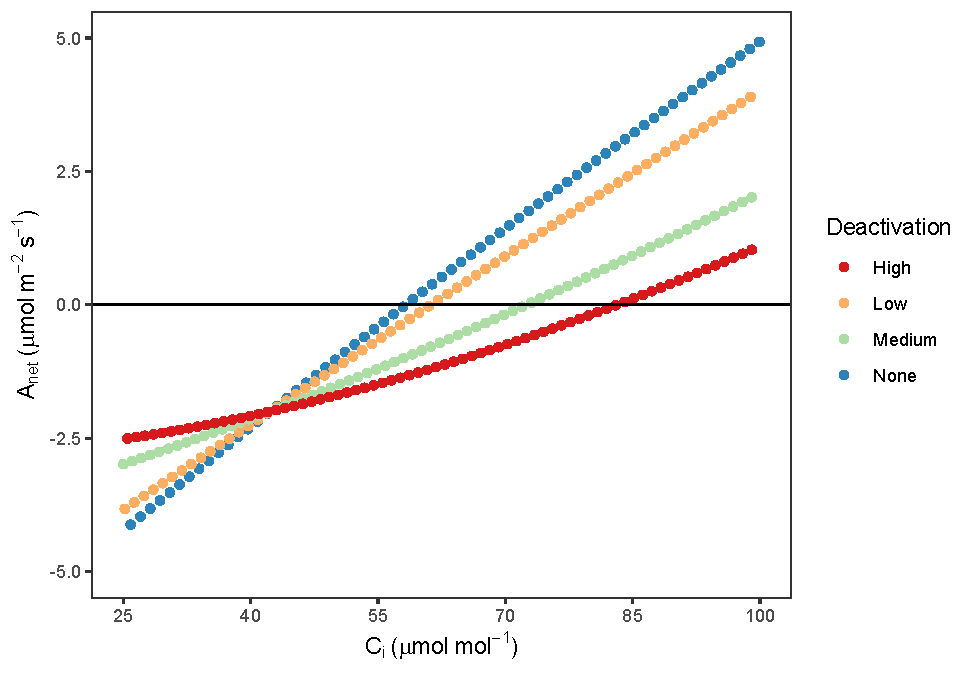
\includegraphics{bookdown_files/figure-latex/anetdecci-1.pdf}
\caption{\label{fig:anetdecci}Rubisco 不同失活程度时 Anet VS Ci}
\end{figure}

\begin{Shaded}
\begin{Highlighting}[]
\NormalTok{AappCc <-}
\StringTok{  }\KeywordTok{ggplot}\NormalTok{(data, }\KeywordTok{aes}\NormalTok{(}\DataTypeTok{x =}\NormalTok{ Ccfull, }\DataTypeTok{y =}\NormalTok{ Aapp, }\DataTypeTok{colour =}\NormalTok{ Deactivation)) }\OperatorTok{+}
\StringTok{  }\KeywordTok{geom_point}\NormalTok{() }\OperatorTok{+}
\StringTok{  }\KeywordTok{labs}\NormalTok{(}\DataTypeTok{x =} \KeywordTok{expression}\NormalTok{(C[c] }\OperatorTok{~}\StringTok{ "("} \OperatorTok{*}\StringTok{ }\NormalTok{mu }\OperatorTok{*}\StringTok{ }\NormalTok{mol }\OperatorTok{~}\StringTok{ }\NormalTok{mol }\OperatorTok{^}\StringTok{ }\NormalTok{\{}
    \DecValTok{-1}
\NormalTok{  \} }\OperatorTok{*}\StringTok{ ")"}\NormalTok{),}
  \DataTypeTok{y =} \KeywordTok{expression}\NormalTok{(A[apparent] }\OperatorTok{~}\StringTok{ "("} \OperatorTok{*}\StringTok{ }\NormalTok{mu }\OperatorTok{*}\StringTok{ }\NormalTok{mol }\OperatorTok{~}\StringTok{ }\NormalTok{m }\OperatorTok{^}\StringTok{ }\NormalTok{\{}
    \DecValTok{-2}
\NormalTok{  \} }\OperatorTok{~}\StringTok{ }\NormalTok{s }\OperatorTok{^}\StringTok{ }\NormalTok{\{}
    \DecValTok{-1}
\NormalTok{  \} }\OperatorTok{*}\StringTok{ ")"}\NormalTok{)) }\OperatorTok{+}
\StringTok{  }\KeywordTok{labs}\NormalTok{(}\DataTypeTok{colour =} \StringTok{'Deactivation'}\NormalTok{) }\OperatorTok{+}
\StringTok{  }\KeywordTok{scale_x_continuous}\NormalTok{(}\DataTypeTok{limits =} \KeywordTok{c}\NormalTok{(}\DecValTok{25}\NormalTok{, }\DecValTok{75}\NormalTok{),}
                     \DataTypeTok{breaks =} \KeywordTok{c}\NormalTok{(}\DecValTok{25}\NormalTok{, }\DecValTok{35}\NormalTok{, }\DecValTok{45}\NormalTok{, }\DecValTok{55}\NormalTok{, }\DecValTok{65}\NormalTok{, }\DecValTok{75}\NormalTok{)) }\OperatorTok{+}
\StringTok{  }\KeywordTok{scale_y_continuous}\NormalTok{(}\DataTypeTok{limits =} \KeywordTok{c}\NormalTok{(}\OperatorTok{-}\DecValTok{5}\NormalTok{, }\DecValTok{5}\NormalTok{)) }\OperatorTok{+}
\StringTok{  }\KeywordTok{scale_colour_brewer}\NormalTok{(}\DataTypeTok{palette =} \StringTok{'Spectral'}\NormalTok{) }\OperatorTok{+}
\StringTok{  }\KeywordTok{geom_hline}\NormalTok{(}\DataTypeTok{yintercept =} \DecValTok{0}\NormalTok{) }\OperatorTok{+}
\StringTok{  }\KeywordTok{theme_bw}\NormalTok{() }\OperatorTok{+}
\StringTok{  }\KeywordTok{theme}\NormalTok{(}\DataTypeTok{panel.grid.major =} \KeywordTok{element_blank}\NormalTok{(),}
        \DataTypeTok{panel.grid.minor =} \KeywordTok{element_blank}\NormalTok{())}
\NormalTok{AappCc}
\end{Highlighting}
\end{Shaded}

\begin{figure}
\centering
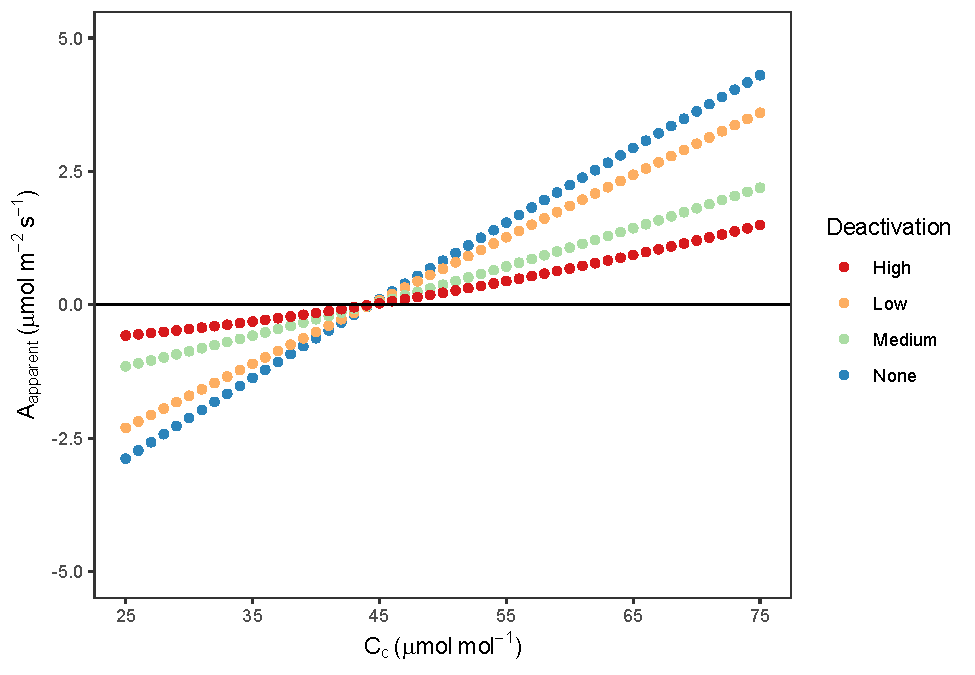
\includegraphics{bookdown_files/figure-latex/aappdeccc-1.pdf}
\caption{\label{fig:aappdeccc}Rubisco 不同失活程度时 Aapp VS Cc}
\end{figure}

\begin{Shaded}
\begin{Highlighting}[]
\NormalTok{AappCi <-}
\StringTok{  }\KeywordTok{ggplot}\NormalTok{(data, }\KeywordTok{aes}\NormalTok{(}\DataTypeTok{x =}\NormalTok{ Cifull, }\DataTypeTok{y =}\NormalTok{ Aapp, }\DataTypeTok{colour =}\NormalTok{ Deactivation)) }\OperatorTok{+}
\StringTok{  }\KeywordTok{geom_point}\NormalTok{() }\OperatorTok{+}
\StringTok{  }\KeywordTok{labs}\NormalTok{(}\DataTypeTok{x =} \KeywordTok{expression}\NormalTok{(C[i] }\OperatorTok{~}\StringTok{ "("} \OperatorTok{*}\StringTok{ }\NormalTok{mu }\OperatorTok{*}\StringTok{ }\NormalTok{mol }\OperatorTok{~}\StringTok{ }\NormalTok{mol }\OperatorTok{^}\StringTok{ }\NormalTok{\{}
    \DecValTok{-1}
\NormalTok{  \} }\OperatorTok{*}\StringTok{ ")"}\NormalTok{),}
  \DataTypeTok{y =} \KeywordTok{expression}\NormalTok{(A[apparent] }\OperatorTok{~}\StringTok{ "("} \OperatorTok{*}\StringTok{ }\NormalTok{mu }\OperatorTok{*}\StringTok{ }\NormalTok{mol }\OperatorTok{~}\StringTok{ }\NormalTok{m }\OperatorTok{^}\StringTok{ }\NormalTok{\{}
    \DecValTok{-2}
\NormalTok{  \} }\OperatorTok{~}\StringTok{ }\NormalTok{s }\OperatorTok{^}\StringTok{ }\NormalTok{\{}
    \DecValTok{-1}
\NormalTok{  \} }\OperatorTok{*}\StringTok{ ")"}\NormalTok{)) }\OperatorTok{+}
\StringTok{  }\KeywordTok{labs}\NormalTok{(}\DataTypeTok{colour =} \StringTok{'Deactivation'}\NormalTok{) }\OperatorTok{+}
\StringTok{  }\KeywordTok{scale_x_continuous}\NormalTok{(}\DataTypeTok{limits =} \KeywordTok{c}\NormalTok{(}\DecValTok{25}\NormalTok{, }\DecValTok{75}\NormalTok{),}
                     \DataTypeTok{breaks =} \KeywordTok{c}\NormalTok{(}\DecValTok{25}\NormalTok{, }\DecValTok{35}\NormalTok{, }\DecValTok{45}\NormalTok{, }\DecValTok{55}\NormalTok{, }\DecValTok{65}\NormalTok{, }\DecValTok{75}\NormalTok{)) }\OperatorTok{+}
\StringTok{  }\KeywordTok{scale_y_continuous}\NormalTok{(}\DataTypeTok{limits =} \KeywordTok{c}\NormalTok{(}\OperatorTok{-}\DecValTok{5}\NormalTok{, }\DecValTok{5}\NormalTok{)) }\OperatorTok{+}
\StringTok{  }\KeywordTok{scale_colour_brewer}\NormalTok{(}\DataTypeTok{palette =} \StringTok{'Spectral'}\NormalTok{) }\OperatorTok{+}
\StringTok{  }\KeywordTok{geom_hline}\NormalTok{(}\DataTypeTok{yintercept =} \DecValTok{0}\NormalTok{) }\OperatorTok{+}
\StringTok{  }\KeywordTok{theme_bw}\NormalTok{() }\OperatorTok{+}
\StringTok{  }\KeywordTok{theme}\NormalTok{(}\DataTypeTok{panel.grid.major =} \KeywordTok{element_blank}\NormalTok{(),}
        \DataTypeTok{panel.grid.minor =} \KeywordTok{element_blank}\NormalTok{())}
\NormalTok{AappCi}
\end{Highlighting}
\end{Shaded}

\begin{figure}
\centering
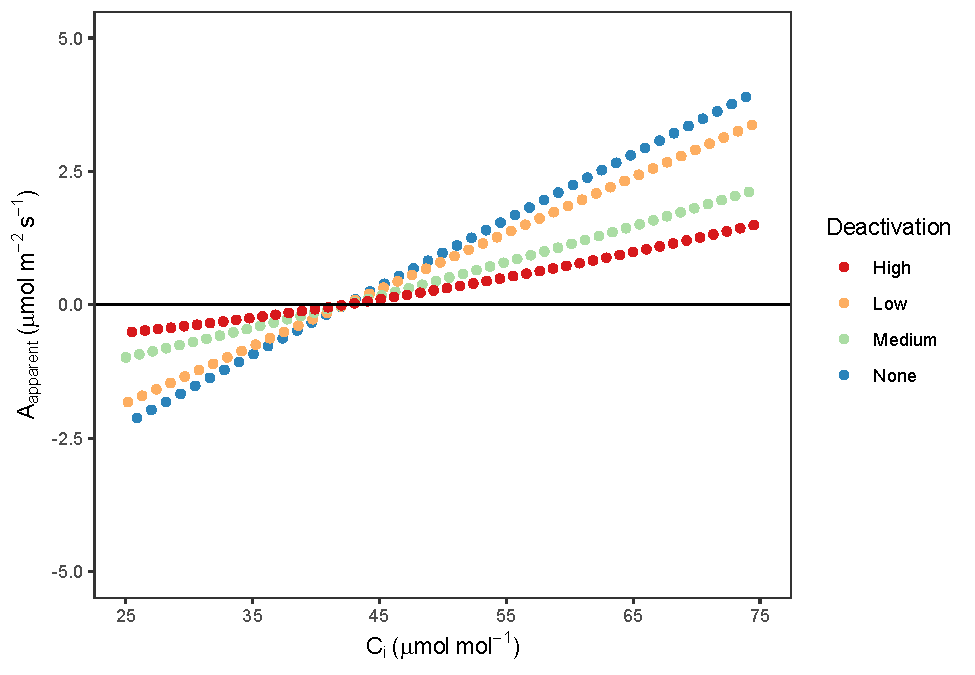
\includegraphics{bookdown_files/figure-latex/aappdecci-1.pdf}
\caption{\label{fig:aappdecci}Rubisco 不同失活程度时 Aapp VS Ci}
\end{figure}

\hypertarget{comp-est-dea}{%
\subsection{不同失活程度下补偿点计算}\label{comp-est-dea}}

此部分内容同未失活状态相似,不在额外介绍,可参考 \ref{gammastar} 内容。

\begin{Shaded}
\begin{Highlighting}[]
\CommentTok{#Gamma}
\CommentTok{# For Ci-based estimates, only use Ci < 100}
\NormalTok{dataCi <-}\StringTok{ }\NormalTok{data[data}\OperatorTok{$}\NormalTok{Cifull }\OperatorTok{<}\StringTok{ }\DecValTok{100}\NormalTok{, ]}
\NormalTok{dataCinone <-}\StringTok{ }\NormalTok{dataCi[dataCi}\OperatorTok{$}\NormalTok{Deactivation }\OperatorTok{==}\StringTok{ "None"}\NormalTok{, ]}
\NormalTok{dataCilow <-}\StringTok{ }\NormalTok{dataCi[dataCi}\OperatorTok{$}\NormalTok{Deactivation }\OperatorTok{==}\StringTok{ "Low"}\NormalTok{, ]}
\NormalTok{dataCimedium <-}\StringTok{ }\NormalTok{dataCi[dataCi}\OperatorTok{$}\NormalTok{Deactivation }\OperatorTok{==}\StringTok{ "Medium"}\NormalTok{, ]}
\NormalTok{dataCihigh <-}\StringTok{ }\NormalTok{dataCi[dataCi}\OperatorTok{$}\NormalTok{Deactivation }\OperatorTok{==}\StringTok{ "High"}\NormalTok{, ]}
\NormalTok{m1 <-}\StringTok{ }\KeywordTok{lm}\NormalTok{(dataCinone}\OperatorTok{$}\NormalTok{Anet }\OperatorTok{~}\StringTok{ }\NormalTok{dataCinone}\OperatorTok{$}\NormalTok{Cifull)}
\KeywordTok{summary}\NormalTok{(m1)}
\end{Highlighting}
\end{Shaded}

\begin{verbatim}
## 
## Call:
## lm(formula = dataCinone$Anet ~ dataCinone$Cifull)
## 
## Residuals:
##      Min       1Q   Median       3Q      Max 
## -0.13165 -0.04518  0.01711  0.05408  0.06699 
## 
## Coefficients:
##                     Estimate Std. Error t value Pr(>|t|)    
## (Intercept)       -7.2248105  0.0199353  -362.4   <2e-16 ***
## dataCinone$Cifull  0.1228632  0.0003089   397.8   <2e-16 ***
## ---
## Signif. codes:  0 '***' 0.001 '**' 0.01 '*' 0.05 '.' 0.1 ' ' 1
## 
## Residual standard error: 0.06081 on 69 degrees of freedom
## Multiple R-squared:  0.9996, Adjusted R-squared:  0.9996 
## F-statistic: 1.582e+05 on 1 and 69 DF,  p-value: < 2.2e-16
\end{verbatim}

\begin{Shaded}
\begin{Highlighting}[]
\NormalTok{Gammanone <-}\StringTok{ }\OperatorTok{-}\NormalTok{m1}\OperatorTok{$}\NormalTok{coefficients[}\DecValTok{1}\NormalTok{] }\OperatorTok{/}\StringTok{ }\NormalTok{m1}\OperatorTok{$}\NormalTok{coefficients[}\DecValTok{2}\NormalTok{]}
\NormalTok{m2 <-}\StringTok{ }\KeywordTok{lm}\NormalTok{(dataCilow}\OperatorTok{$}\NormalTok{Anet }\OperatorTok{~}\StringTok{ }\NormalTok{dataCilow}\OperatorTok{$}\NormalTok{Cifull)}
\KeywordTok{summary}\NormalTok{(m2)}
\end{Highlighting}
\end{Shaded}

\begin{verbatim}
## 
## Call:
## lm(formula = dataCilow$Anet ~ dataCilow$Cifull)
## 
## Residuals:
##       Min        1Q    Median        3Q       Max 
## -0.034896 -0.011957  0.004499  0.014311  0.017726 
## 
## Coefficients:
##                    Estimate Std. Error t value Pr(>|t|)    
## (Intercept)      -6.444e+00  5.343e-03   -1206   <2e-16 ***
## dataCilow$Cifull  1.049e-01  8.341e-05    1258   <2e-16 ***
## ---
## Signif. codes:  0 '***' 0.001 '**' 0.01 '*' 0.05 '.' 0.1 ' ' 1
## 
## Residual standard error: 0.01609 on 69 degrees of freedom
## Multiple R-squared:      1,  Adjusted R-squared:      1 
## F-statistic: 1.582e+06 on 1 and 69 DF,  p-value: < 2.2e-16
\end{verbatim}

\begin{Shaded}
\begin{Highlighting}[]
\NormalTok{Gammalow <-}\StringTok{ }\OperatorTok{-}\NormalTok{m2}\OperatorTok{$}\NormalTok{coefficients[}\DecValTok{1}\NormalTok{] }\OperatorTok{/}\StringTok{ }\NormalTok{m2}\OperatorTok{$}\NormalTok{coefficients[}\DecValTok{2}\NormalTok{]}
\NormalTok{m3 <-}\StringTok{ }\KeywordTok{lm}\NormalTok{(dataCimedium}\OperatorTok{$}\NormalTok{Anet }\OperatorTok{~}\StringTok{ }\NormalTok{dataCimedium}\OperatorTok{$}\NormalTok{Cifull)}
\KeywordTok{summary}\NormalTok{(m3)}
\end{Highlighting}
\end{Shaded}

\begin{verbatim}
## 
## Call:
## lm(formula = dataCimedium$Anet ~ dataCimedium$Cifull)
## 
## Residuals:
##      Min       1Q   Median       3Q      Max 
## -0.09168 -0.07338 -0.02281  0.05893  0.18150 
## 
## Coefficients:
##                       Estimate Std. Error t value Pr(>|t|)    
## (Intercept)         -4.8015337  0.0277371  -173.1   <2e-16 ***
## dataCimedium$Cifull  0.0671064  0.0004311   155.7   <2e-16 ***
## ---
## Signif. codes:  0 '***' 0.001 '**' 0.01 '*' 0.05 '.' 0.1 ' ' 1
## 
## Residual standard error: 0.0832 on 71 degrees of freedom
## Multiple R-squared:  0.9971, Adjusted R-squared:  0.997 
## F-statistic: 2.423e+04 on 1 and 71 DF,  p-value: < 2.2e-16
\end{verbatim}

\begin{Shaded}
\begin{Highlighting}[]
\NormalTok{Gammamedium <-}\StringTok{ }\OperatorTok{-}\NormalTok{m3}\OperatorTok{$}\NormalTok{coefficients[}\DecValTok{1}\NormalTok{] }\OperatorTok{/}\StringTok{ }\NormalTok{m3}\OperatorTok{$}\NormalTok{coefficients[}\DecValTok{2}\NormalTok{]}
\NormalTok{m4 <-}\StringTok{ }\KeywordTok{lm}\NormalTok{(dataCihigh}\OperatorTok{$}\NormalTok{Anet }\OperatorTok{~}\StringTok{ }\NormalTok{dataCihigh}\OperatorTok{$}\NormalTok{Cifull)}
\KeywordTok{summary}\NormalTok{(m4)}
\end{Highlighting}
\end{Shaded}

\begin{verbatim}
## 
## Call:
## lm(formula = dataCihigh$Anet ~ dataCihigh$Cifull)
## 
## Residuals:
##      Min       1Q   Median       3Q      Max 
## -0.15430 -0.12508 -0.03863  0.10156  0.30621 
## 
## Coefficients:
##                     Estimate Std. Error t value Pr(>|t|)    
## (Intercept)       -3.9450658  0.0467537  -84.38   <2e-16 ***
## dataCihigh$Cifull  0.0473551  0.0007255   65.27   <2e-16 ***
## ---
## Signif. codes:  0 '***' 0.001 '**' 0.01 '*' 0.05 '.' 0.1 ' ' 1
## 
## Residual standard error: 0.1399 on 72 degrees of freedom
## Multiple R-squared:  0.9834, Adjusted R-squared:  0.9831 
## F-statistic:  4260 on 1 and 72 DF,  p-value: < 2.2e-16
\end{verbatim}

\begin{Shaded}
\begin{Highlighting}[]
\NormalTok{Gammahigh <-}\StringTok{ }\OperatorTok{-}\NormalTok{m4}\OperatorTok{$}\NormalTok{coefficients[}\DecValTok{1}\NormalTok{] }\OperatorTok{/}\StringTok{ }\NormalTok{m4}\OperatorTok{$}\NormalTok{coefficients[}\DecValTok{2}\NormalTok{]}

\NormalTok{GammaCi <-}\StringTok{ }\KeywordTok{c}\NormalTok{(Gammanone, Gammalow, Gammamedium, Gammahigh)}

\CommentTok{# For Cc-based estimates, only use Cc < 75}
\NormalTok{dataCc <-}\StringTok{ }\NormalTok{data[data}\OperatorTok{$}\NormalTok{Ccfull }\OperatorTok{<}\StringTok{ }\DecValTok{75}\NormalTok{, ]}
\NormalTok{dataCcnone <-}\StringTok{ }\NormalTok{dataCc[dataCc}\OperatorTok{$}\NormalTok{Deactivation }\OperatorTok{==}\StringTok{ "None"}\NormalTok{, ]}
\NormalTok{dataCclow <-}\StringTok{ }\NormalTok{dataCc[dataCc}\OperatorTok{$}\NormalTok{Deactivation }\OperatorTok{==}\StringTok{ "Low"}\NormalTok{, ]}
\NormalTok{dataCcmedium <-}\StringTok{ }\NormalTok{dataCc[dataCc}\OperatorTok{$}\NormalTok{Deactivation }\OperatorTok{==}\StringTok{ "Medium"}\NormalTok{, ]}
\NormalTok{dataCchigh <-}\StringTok{ }\NormalTok{dataCc[dataCc}\OperatorTok{$}\NormalTok{Deactivation }\OperatorTok{==}\StringTok{ "High"}\NormalTok{, ]}
\NormalTok{m1 <-}\StringTok{ }\KeywordTok{lm}\NormalTok{(dataCcnone}\OperatorTok{$}\NormalTok{Anet }\OperatorTok{~}\StringTok{ }\NormalTok{dataCcnone}\OperatorTok{$}\NormalTok{Ccfull)}
\KeywordTok{summary}\NormalTok{(m1)}
\end{Highlighting}
\end{Shaded}

\begin{verbatim}
## 
## Call:
## lm(formula = dataCcnone$Anet ~ dataCcnone$Ccfull)
## 
## Residuals:
##       Min        1Q    Median        3Q       Max 
## -0.075648 -0.025444  0.009857  0.031706  0.039431 
## 
## Coefficients:
##                     Estimate Std. Error t value Pr(>|t|)    
## (Intercept)       -8.4062011  0.0181852  -462.3   <2e-16 ***
## dataCcnone$Ccfull  0.1438710  0.0003527   407.9   <2e-16 ***
## ---
## Signif. codes:  0 '***' 0.001 '**' 0.01 '*' 0.05 '.' 0.1 ' ' 1
## 
## Residual standard error: 0.03599 on 48 degrees of freedom
## Multiple R-squared:  0.9997, Adjusted R-squared:  0.9997 
## F-statistic: 1.664e+05 on 1 and 48 DF,  p-value: < 2.2e-16
\end{verbatim}

\begin{Shaded}
\begin{Highlighting}[]
\NormalTok{Gammanone <-}\StringTok{ }\OperatorTok{-}\NormalTok{m1}\OperatorTok{$}\NormalTok{coefficients[}\DecValTok{1}\NormalTok{] }\OperatorTok{/}\StringTok{ }\NormalTok{m1}\OperatorTok{$}\NormalTok{coefficients[}\DecValTok{2}\NormalTok{]}
\NormalTok{m2 <-}\StringTok{ }\KeywordTok{lm}\NormalTok{(dataCclow}\OperatorTok{$}\NormalTok{Anet }\OperatorTok{~}\StringTok{ }\NormalTok{dataCclow}\OperatorTok{$}\NormalTok{Ccfull)}
\KeywordTok{summary}\NormalTok{(m2)}
\end{Highlighting}
\end{Shaded}

\begin{verbatim}
## 
## Call:
## lm(formula = dataCclow$Anet ~ dataCclow$Ccfull)
## 
## Residuals:
##       Min        1Q    Median        3Q       Max 
## -0.019617 -0.006598  0.002556  0.008222  0.010225 
## 
## Coefficients:
##                    Estimate Std. Error t value Pr(>|t|)    
## (Intercept)      -7.243e+00  4.716e-03   -1536   <2e-16 ***
## dataCclow$Ccfull  1.182e-01  9.146e-05    1292   <2e-16 ***
## ---
## Signif. codes:  0 '***' 0.001 '**' 0.01 '*' 0.05 '.' 0.1 ' ' 1
## 
## Residual standard error: 0.009333 on 48 degrees of freedom
## Multiple R-squared:      1,  Adjusted R-squared:      1 
## F-statistic: 1.67e+06 on 1 and 48 DF,  p-value: < 2.2e-16
\end{verbatim}

\begin{Shaded}
\begin{Highlighting}[]
\NormalTok{Gammalow <-}\StringTok{ }\OperatorTok{-}\NormalTok{m2}\OperatorTok{$}\NormalTok{coefficients[}\DecValTok{1}\NormalTok{] }\OperatorTok{/}\StringTok{ }\NormalTok{m2}\OperatorTok{$}\NormalTok{coefficients[}\DecValTok{2}\NormalTok{]}
\NormalTok{m3 <-}\StringTok{ }\KeywordTok{lm}\NormalTok{(dataCcmedium}\OperatorTok{$}\NormalTok{Anet }\OperatorTok{~}\StringTok{ }\NormalTok{dataCcmedium}\OperatorTok{$}\NormalTok{Ccfull)}
\KeywordTok{summary}\NormalTok{(m3)}
\end{Highlighting}
\end{Shaded}

\begin{verbatim}
## 
## Call:
## lm(formula = dataCcmedium$Anet ~ dataCcmedium$Ccfull)
## 
## Residuals:
##      Min       1Q   Median       3Q      Max 
## -0.04819 -0.03875 -0.01205  0.03109  0.09244 
## 
## Coefficients:
##                      Estimate Std. Error t value Pr(>|t|)    
## (Intercept)         -4.917283   0.022223  -221.3   <2e-16 ***
## dataCcmedium$Ccfull  0.066832   0.000431   155.1   <2e-16 ***
## ---
## Signif. codes:  0 '***' 0.001 '**' 0.01 '*' 0.05 '.' 0.1 ' ' 1
## 
## Residual standard error: 0.04398 on 48 degrees of freedom
## Multiple R-squared:  0.998,  Adjusted R-squared:  0.998 
## F-statistic: 2.404e+04 on 1 and 48 DF,  p-value: < 2.2e-16
\end{verbatim}

\begin{Shaded}
\begin{Highlighting}[]
\NormalTok{Gammamedium <-}\StringTok{ }\OperatorTok{-}\NormalTok{m3}\OperatorTok{$}\NormalTok{coefficients[}\DecValTok{1}\NormalTok{] }\OperatorTok{/}\StringTok{ }\NormalTok{m3}\OperatorTok{$}\NormalTok{coefficients[}\DecValTok{2}\NormalTok{]}
\NormalTok{m4 <-}\StringTok{ }\KeywordTok{lm}\NormalTok{(dataCchigh}\OperatorTok{$}\NormalTok{Anet }\OperatorTok{~}\StringTok{ }\NormalTok{dataCchigh}\OperatorTok{$}\NormalTok{Ccfull)}
\KeywordTok{summary}\NormalTok{(m4)}
\end{Highlighting}
\end{Shaded}

\begin{verbatim}
## 
## Call:
## lm(formula = dataCchigh$Anet ~ dataCchigh$Ccfull)
## 
## Residuals:
##      Min       1Q   Median       3Q      Max 
## -0.07739 -0.06223 -0.01935  0.04994  0.14847 
## 
## Coefficients:
##                     Estimate Std. Error t value Pr(>|t|)    
## (Intercept)       -3.7543099  0.0356922 -105.19   <2e-16 ***
## dataCchigh$Ccfull  0.0411528  0.0006922   59.45   <2e-16 ***
## ---
## Signif. codes:  0 '***' 0.001 '**' 0.01 '*' 0.05 '.' 0.1 ' ' 1
## 
## Residual standard error: 0.07064 on 48 degrees of freedom
## Multiple R-squared:  0.9866, Adjusted R-squared:  0.9863 
## F-statistic:  3534 on 1 and 48 DF,  p-value: < 2.2e-16
\end{verbatim}

\begin{Shaded}
\begin{Highlighting}[]
\NormalTok{Gammahigh <-}\StringTok{ }\OperatorTok{-}\NormalTok{m4}\OperatorTok{$}\NormalTok{coefficients[}\DecValTok{1}\NormalTok{] }\OperatorTok{/}\StringTok{ }\NormalTok{m4}\OperatorTok{$}\NormalTok{coefficients[}\DecValTok{2}\NormalTok{]}

\NormalTok{GammaCc <-}\StringTok{ }\KeywordTok{c}\NormalTok{(Gammanone, Gammalow, Gammamedium, Gammahigh)}

\CommentTok{#GammaStar}
\CommentTok{# For Ci-based estimates, only use Ci < 100}
\NormalTok{dataCi <-}\StringTok{ }\NormalTok{data[data}\OperatorTok{$}\NormalTok{Cifull }\OperatorTok{<}\StringTok{ }\DecValTok{100}\NormalTok{, ]}
\NormalTok{dataCinone <-}\StringTok{ }\NormalTok{dataCi[dataCi}\OperatorTok{$}\NormalTok{Deactivation }\OperatorTok{==}\StringTok{ "None"}\NormalTok{, ]}
\NormalTok{dataCilow <-}\StringTok{ }\NormalTok{dataCi[dataCi}\OperatorTok{$}\NormalTok{Deactivation }\OperatorTok{==}\StringTok{ "Low"}\NormalTok{, ]}
\NormalTok{dataCimedium <-}\StringTok{ }\NormalTok{dataCi[dataCi}\OperatorTok{$}\NormalTok{Deactivation }\OperatorTok{==}\StringTok{ "Medium"}\NormalTok{, ]}
\NormalTok{dataCihigh <-}\StringTok{ }\NormalTok{dataCi[dataCi}\OperatorTok{$}\NormalTok{Deactivation }\OperatorTok{==}\StringTok{ "High"}\NormalTok{, ]}
\NormalTok{m1 <-}\StringTok{ }\KeywordTok{lm}\NormalTok{(dataCinone}\OperatorTok{$}\NormalTok{Aapp }\OperatorTok{~}\StringTok{ }\NormalTok{dataCinone}\OperatorTok{$}\NormalTok{Cifull)}
\KeywordTok{summary}\NormalTok{(m1)}
\end{Highlighting}
\end{Shaded}

\begin{verbatim}
## 
## Call:
## lm(formula = dataCinone$Aapp ~ dataCinone$Cifull)
## 
## Residuals:
##      Min       1Q   Median       3Q      Max 
## -0.13165 -0.04518  0.01711  0.05408  0.06699 
## 
## Coefficients:
##                     Estimate Std. Error t value Pr(>|t|)    
## (Intercept)       -5.2248105  0.0199353  -262.1   <2e-16 ***
## dataCinone$Cifull  0.1228632  0.0003089   397.8   <2e-16 ***
## ---
## Signif. codes:  0 '***' 0.001 '**' 0.01 '*' 0.05 '.' 0.1 ' ' 1
## 
## Residual standard error: 0.06081 on 69 degrees of freedom
## Multiple R-squared:  0.9996, Adjusted R-squared:  0.9996 
## F-statistic: 1.582e+05 on 1 and 69 DF,  p-value: < 2.2e-16
\end{verbatim}

\begin{Shaded}
\begin{Highlighting}[]
\NormalTok{Gammastarnone <-}\StringTok{ }\OperatorTok{-}\NormalTok{m1}\OperatorTok{$}\NormalTok{coefficients[}\DecValTok{1}\NormalTok{] }\OperatorTok{/}\StringTok{ }\NormalTok{m1}\OperatorTok{$}\NormalTok{coefficients[}\DecValTok{2}\NormalTok{]}
\NormalTok{m2 <-}\StringTok{ }\KeywordTok{lm}\NormalTok{(dataCilow}\OperatorTok{$}\NormalTok{Aapp }\OperatorTok{~}\StringTok{ }\NormalTok{dataCilow}\OperatorTok{$}\NormalTok{Cifull)}
\KeywordTok{summary}\NormalTok{(m2)}
\end{Highlighting}
\end{Shaded}

\begin{verbatim}
## 
## Call:
## lm(formula = dataCilow$Aapp ~ dataCilow$Cifull)
## 
## Residuals:
##       Min        1Q    Median        3Q       Max 
## -0.034896 -0.011957  0.004499  0.014311  0.017726 
## 
## Coefficients:
##                    Estimate Std. Error t value Pr(>|t|)    
## (Intercept)      -4.444e+00  5.343e-03  -831.7   <2e-16 ***
## dataCilow$Cifull  1.049e-01  8.341e-05  1257.8   <2e-16 ***
## ---
## Signif. codes:  0 '***' 0.001 '**' 0.01 '*' 0.05 '.' 0.1 ' ' 1
## 
## Residual standard error: 0.01609 on 69 degrees of freedom
## Multiple R-squared:      1,  Adjusted R-squared:      1 
## F-statistic: 1.582e+06 on 1 and 69 DF,  p-value: < 2.2e-16
\end{verbatim}

\begin{Shaded}
\begin{Highlighting}[]
\NormalTok{Gammastarlow <-}\StringTok{ }\OperatorTok{-}\NormalTok{m2}\OperatorTok{$}\NormalTok{coefficients[}\DecValTok{1}\NormalTok{] }\OperatorTok{/}\StringTok{ }\NormalTok{m2}\OperatorTok{$}\NormalTok{coefficients[}\DecValTok{2}\NormalTok{]}
\NormalTok{m3 <-}\StringTok{ }\KeywordTok{lm}\NormalTok{(dataCimedium}\OperatorTok{$}\NormalTok{Aapp }\OperatorTok{~}\StringTok{ }\NormalTok{dataCimedium}\OperatorTok{$}\NormalTok{Cifull)}
\KeywordTok{summary}\NormalTok{(m3)}
\end{Highlighting}
\end{Shaded}

\begin{verbatim}
## 
## Call:
## lm(formula = dataCimedium$Aapp ~ dataCimedium$Cifull)
## 
## Residuals:
##      Min       1Q   Median       3Q      Max 
## -0.09168 -0.07338 -0.02281  0.05893  0.18150 
## 
## Coefficients:
##                       Estimate Std. Error t value Pr(>|t|)    
## (Intercept)         -2.8015337  0.0277371  -101.0   <2e-16 ***
## dataCimedium$Cifull  0.0671064  0.0004311   155.7   <2e-16 ***
## ---
## Signif. codes:  0 '***' 0.001 '**' 0.01 '*' 0.05 '.' 0.1 ' ' 1
## 
## Residual standard error: 0.0832 on 71 degrees of freedom
## Multiple R-squared:  0.9971, Adjusted R-squared:  0.997 
## F-statistic: 2.423e+04 on 1 and 71 DF,  p-value: < 2.2e-16
\end{verbatim}

\begin{Shaded}
\begin{Highlighting}[]
\NormalTok{Gammastarmedium <-}\StringTok{ }\OperatorTok{-}\NormalTok{m3}\OperatorTok{$}\NormalTok{coefficients[}\DecValTok{1}\NormalTok{] }\OperatorTok{/}\StringTok{ }\NormalTok{m3}\OperatorTok{$}\NormalTok{coefficients[}\DecValTok{2}\NormalTok{]}
\NormalTok{m4 <-}\StringTok{ }\KeywordTok{lm}\NormalTok{(dataCihigh}\OperatorTok{$}\NormalTok{Aapp }\OperatorTok{~}\StringTok{ }\NormalTok{dataCihigh}\OperatorTok{$}\NormalTok{Cifull)}
\KeywordTok{summary}\NormalTok{(m4)}
\end{Highlighting}
\end{Shaded}

\begin{verbatim}
## 
## Call:
## lm(formula = dataCihigh$Aapp ~ dataCihigh$Cifull)
## 
## Residuals:
##      Min       1Q   Median       3Q      Max 
## -0.15430 -0.12508 -0.03863  0.10156  0.30621 
## 
## Coefficients:
##                     Estimate Std. Error t value Pr(>|t|)    
## (Intercept)       -1.9450658  0.0467537  -41.60   <2e-16 ***
## dataCihigh$Cifull  0.0473551  0.0007255   65.27   <2e-16 ***
## ---
## Signif. codes:  0 '***' 0.001 '**' 0.01 '*' 0.05 '.' 0.1 ' ' 1
## 
## Residual standard error: 0.1399 on 72 degrees of freedom
## Multiple R-squared:  0.9834, Adjusted R-squared:  0.9831 
## F-statistic:  4260 on 1 and 72 DF,  p-value: < 2.2e-16
\end{verbatim}

\begin{Shaded}
\begin{Highlighting}[]
\NormalTok{Gammastarhigh <-}\StringTok{ }\OperatorTok{-}\NormalTok{m4}\OperatorTok{$}\NormalTok{coefficients[}\DecValTok{1}\NormalTok{] }\OperatorTok{/}\StringTok{ }\NormalTok{m4}\OperatorTok{$}\NormalTok{coefficients[}\DecValTok{2}\NormalTok{]}

\NormalTok{GammastarCi <-}
\StringTok{  }\KeywordTok{c}\NormalTok{(Gammastarnone, Gammastarlow, Gammastarmedium, Gammastarhigh)}

\CommentTok{# For Cc-based estimates, only use Cc < 75}
\NormalTok{dataCc <-}\StringTok{ }\NormalTok{data[data}\OperatorTok{$}\NormalTok{Ccfull }\OperatorTok{<}\StringTok{ }\DecValTok{75}\NormalTok{, ]}
\NormalTok{dataCcnone <-}\StringTok{ }\NormalTok{dataCc[dataCc}\OperatorTok{$}\NormalTok{Deactivation }\OperatorTok{==}\StringTok{ "None"}\NormalTok{, ]}
\NormalTok{dataCclow <-}\StringTok{ }\NormalTok{dataCc[dataCc}\OperatorTok{$}\NormalTok{Deactivation }\OperatorTok{==}\StringTok{ "Low"}\NormalTok{, ]}
\NormalTok{dataCcmedium <-}\StringTok{ }\NormalTok{dataCc[dataCc}\OperatorTok{$}\NormalTok{Deactivation }\OperatorTok{==}\StringTok{ "Medium"}\NormalTok{, ]}
\NormalTok{dataCchigh <-}\StringTok{ }\NormalTok{dataCc[dataCc}\OperatorTok{$}\NormalTok{Deactivation }\OperatorTok{==}\StringTok{ "High"}\NormalTok{, ]}
\NormalTok{m1 <-}\StringTok{ }\KeywordTok{lm}\NormalTok{(dataCcnone}\OperatorTok{$}\NormalTok{Aapp }\OperatorTok{~}\StringTok{ }\NormalTok{dataCcnone}\OperatorTok{$}\NormalTok{Ccfull)}
\KeywordTok{summary}\NormalTok{(m1)}
\end{Highlighting}
\end{Shaded}

\begin{verbatim}
## 
## Call:
## lm(formula = dataCcnone$Aapp ~ dataCcnone$Ccfull)
## 
## Residuals:
##       Min        1Q    Median        3Q       Max 
## -0.075648 -0.025444  0.009857  0.031706  0.039431 
## 
## Coefficients:
##                     Estimate Std. Error t value Pr(>|t|)    
## (Intercept)       -6.4062011  0.0181852  -352.3   <2e-16 ***
## dataCcnone$Ccfull  0.1438710  0.0003527   407.9   <2e-16 ***
## ---
## Signif. codes:  0 '***' 0.001 '**' 0.01 '*' 0.05 '.' 0.1 ' ' 1
## 
## Residual standard error: 0.03599 on 48 degrees of freedom
## Multiple R-squared:  0.9997, Adjusted R-squared:  0.9997 
## F-statistic: 1.664e+05 on 1 and 48 DF,  p-value: < 2.2e-16
\end{verbatim}

\begin{Shaded}
\begin{Highlighting}[]
\NormalTok{Gammastarnone <-}\StringTok{ }\OperatorTok{-}\NormalTok{m1}\OperatorTok{$}\NormalTok{coefficients[}\DecValTok{1}\NormalTok{] }\OperatorTok{/}\StringTok{ }\NormalTok{m1}\OperatorTok{$}\NormalTok{coefficients[}\DecValTok{2}\NormalTok{]}
\NormalTok{m2 <-}\StringTok{ }\KeywordTok{lm}\NormalTok{(dataCclow}\OperatorTok{$}\NormalTok{Aapp }\OperatorTok{~}\StringTok{ }\NormalTok{dataCclow}\OperatorTok{$}\NormalTok{Ccfull)}
\KeywordTok{summary}\NormalTok{(m2)}
\end{Highlighting}
\end{Shaded}

\begin{verbatim}
## 
## Call:
## lm(formula = dataCclow$Aapp ~ dataCclow$Ccfull)
## 
## Residuals:
##       Min        1Q    Median        3Q       Max 
## -0.019617 -0.006598  0.002556  0.008222  0.010225 
## 
## Coefficients:
##                    Estimate Std. Error t value Pr(>|t|)    
## (Intercept)      -5.243e+00  4.716e-03   -1112   <2e-16 ***
## dataCclow$Ccfull  1.182e-01  9.146e-05    1292   <2e-16 ***
## ---
## Signif. codes:  0 '***' 0.001 '**' 0.01 '*' 0.05 '.' 0.1 ' ' 1
## 
## Residual standard error: 0.009333 on 48 degrees of freedom
## Multiple R-squared:      1,  Adjusted R-squared:      1 
## F-statistic: 1.67e+06 on 1 and 48 DF,  p-value: < 2.2e-16
\end{verbatim}

\begin{Shaded}
\begin{Highlighting}[]
\NormalTok{Gammastarlow <-}\StringTok{ }\OperatorTok{-}\NormalTok{m2}\OperatorTok{$}\NormalTok{coefficients[}\DecValTok{1}\NormalTok{] }\OperatorTok{/}\StringTok{ }\NormalTok{m2}\OperatorTok{$}\NormalTok{coefficients[}\DecValTok{2}\NormalTok{]}
\NormalTok{m3 <-}\StringTok{ }\KeywordTok{lm}\NormalTok{(dataCcmedium}\OperatorTok{$}\NormalTok{Aapp }\OperatorTok{~}\StringTok{ }\NormalTok{dataCcmedium}\OperatorTok{$}\NormalTok{Ccfull)}
\KeywordTok{summary}\NormalTok{(m3)}
\end{Highlighting}
\end{Shaded}

\begin{verbatim}
## 
## Call:
## lm(formula = dataCcmedium$Aapp ~ dataCcmedium$Ccfull)
## 
## Residuals:
##      Min       1Q   Median       3Q      Max 
## -0.04819 -0.03875 -0.01205  0.03109  0.09244 
## 
## Coefficients:
##                      Estimate Std. Error t value Pr(>|t|)    
## (Intercept)         -2.917283   0.022223  -131.3   <2e-16 ***
## dataCcmedium$Ccfull  0.066832   0.000431   155.1   <2e-16 ***
## ---
## Signif. codes:  0 '***' 0.001 '**' 0.01 '*' 0.05 '.' 0.1 ' ' 1
## 
## Residual standard error: 0.04398 on 48 degrees of freedom
## Multiple R-squared:  0.998,  Adjusted R-squared:  0.998 
## F-statistic: 2.404e+04 on 1 and 48 DF,  p-value: < 2.2e-16
\end{verbatim}

\begin{Shaded}
\begin{Highlighting}[]
\NormalTok{Gammastarmedium <-}\StringTok{ }\OperatorTok{-}\NormalTok{m3}\OperatorTok{$}\NormalTok{coefficients[}\DecValTok{1}\NormalTok{] }\OperatorTok{/}\StringTok{ }\NormalTok{m3}\OperatorTok{$}\NormalTok{coefficients[}\DecValTok{2}\NormalTok{]}
\NormalTok{m4 <-}\StringTok{ }\KeywordTok{lm}\NormalTok{(dataCchigh}\OperatorTok{$}\NormalTok{Aapp }\OperatorTok{~}\StringTok{ }\NormalTok{dataCchigh}\OperatorTok{$}\NormalTok{Ccfull)}
\KeywordTok{summary}\NormalTok{(m4)}
\end{Highlighting}
\end{Shaded}

\begin{verbatim}
## 
## Call:
## lm(formula = dataCchigh$Aapp ~ dataCchigh$Ccfull)
## 
## Residuals:
##      Min       1Q   Median       3Q      Max 
## -0.07739 -0.06223 -0.01935  0.04994  0.14847 
## 
## Coefficients:
##                     Estimate Std. Error t value Pr(>|t|)    
## (Intercept)       -1.7543099  0.0356922  -49.15   <2e-16 ***
## dataCchigh$Ccfull  0.0411528  0.0006922   59.45   <2e-16 ***
## ---
## Signif. codes:  0 '***' 0.001 '**' 0.01 '*' 0.05 '.' 0.1 ' ' 1
## 
## Residual standard error: 0.07064 on 48 degrees of freedom
## Multiple R-squared:  0.9866, Adjusted R-squared:  0.9863 
## F-statistic:  3534 on 1 and 48 DF,  p-value: < 2.2e-16
\end{verbatim}

\begin{Shaded}
\begin{Highlighting}[]
\NormalTok{Gammastarhigh <-}\StringTok{ }\OperatorTok{-}\NormalTok{m4}\OperatorTok{$}\NormalTok{coefficients[}\DecValTok{1}\NormalTok{] }\OperatorTok{/}\StringTok{ }\NormalTok{m4}\OperatorTok{$}\NormalTok{coefficients[}\DecValTok{2}\NormalTok{]}

\NormalTok{GammastarCc <-}
\StringTok{  }\KeywordTok{c}\NormalTok{(Gammastarnone, Gammastarlow, Gammastarmedium, Gammastarhigh)}

\NormalTok{Deactivation2 <-}\StringTok{ }\KeywordTok{c}\NormalTok{(}\StringTok{"None"}\NormalTok{, }\StringTok{"Low"}\NormalTok{, }\StringTok{"Medium"}\NormalTok{, }\StringTok{"High"}\NormalTok{)}
\NormalTok{RAScomps <-}
\StringTok{  }\KeywordTok{as.data.frame}\NormalTok{(}\KeywordTok{cbind}\NormalTok{(Deactivation2, GammaCc, GammaCi, GammastarCc, GammastarCi))}
\KeywordTok{write.csv}\NormalTok{(RAScomps, }\StringTok{"./data/RAScomps.csv"}\NormalTok{)}
\end{Highlighting}
\end{Shaded}

\hypertarget{diffu-limi}{%
\section{时间延迟的扩散限制}\label{diffu-limi}}

对于扩散限制,下面的内容比较了多速率 RACiR 和标准 ACi 曲线的差别,比较实在有光呼吸和没有光呼吸的两种情况。对于没有扩散限制的表观光合速,采用了已知质量的碱石灰药品,放置于 1.7 ml 的微量离心管内,然后将其置于荧光叶室内部模拟叶片,此时叶室环境控制与其他实验不同,此时不再控制 H2OR。RACiR 测试从 500 到 0 的变化,不同样品的测量是随机的。

下面内容采用了一定的假设,来计算扩散的时间。

\begin{Shaded}
\begin{Highlighting}[]
\CommentTok{#Equations from Campbell & Norman, 1998}
\CommentTok{#We are taking a simple approach to calculating diffusion times.}
\CommentTok{#Here we make the simplifying assumption that diffusion is pure, planar}
\CommentTok{#Diffusion, such that:}
\CommentTok{#gtot = phat * D / deltaZ}
\CommentTok{#where gtot is total conductance, phat is molar density of air in mol /m^3,}
\CommentTok{#D is diffusion coefficient in m2/s, deltaZ is pathlength in m}
\CommentTok{#Since PV = NRT, N/V = P/RT}
\CommentTok{#T in K, R in J K-1 mol-1, P in Pa}

\CommentTok{#phat = Patm/(RT)}
\NormalTok{phat =}\StringTok{ }\DecValTok{100000} \OperatorTok{/}\StringTok{ }\NormalTok{(}\FloatTok{8.314} \OperatorTok{*}\StringTok{ }\FloatTok{298.15}\NormalTok{)}

\CommentTok{#We also assume a linear pathlength}
\CommentTok{#Note, if diffusion is nonlinear or nonplanar, it will affect the value determined}
\CommentTok{#for D from this equation.}

\CommentTok{#D = gtot * deltaZ / phat}

\CommentTok{#Diffusion time, t, varies with D and deltaZ such that:}

\CommentTok{#t = (deltaZ)^2 / D}

\CommentTok{#So}

\CommentTok{#t = (deltaZ)^2 / (gtot * deltaZ / phat)}

\CommentTok{#If we assume mean diffusion pathlength of 1/2 lamina thickness,}
\CommentTok{#then Onoda et al. 2011 lamina thicknesses of: median 0.22 mm (0.11 to 0.74 for 95% CI)}
\CommentTok{#becomes 0.11 mm (0.055 to 0.37) for estimated deltaZ}

\CommentTok{#Convert pathlength to m}
\NormalTok{dZlow <-}\StringTok{ }\FloatTok{0.055} \OperatorTok{/}\StringTok{ }\DecValTok{1000}
\NormalTok{dZmedian <-}\StringTok{ }\FloatTok{0.11} \OperatorTok{/}\StringTok{ }\DecValTok{1000}
\NormalTok{dZhigh <-}\StringTok{ }\FloatTok{0.37} \OperatorTok{/}\StringTok{ }\DecValTok{1000}
\end{Highlighting}
\end{Shaded}

下面的内容是对边界层导度和气孔导度等赋值,由此而计算出其他所需要的参数:

\begin{Shaded}
\begin{Highlighting}[]
\CommentTok{#Mesophyll Conductance}
\NormalTok{BLC <-}\StringTok{ }\DecValTok{2} \CommentTok{#mol m-2 s-1}
\NormalTok{gsw <-}\StringTok{ }\FloatTok{0.4} \CommentTok{#mol m-2 s-1}

\CommentTok{# 无限制的叶肉导度,并以此计算ci等}
\NormalTok{gm1 <-}\StringTok{ }\DecValTok{1} \CommentTok{#mol m-2 s-1}
\NormalTok{Ci1 <-}\StringTok{ }\NormalTok{A }\OperatorTok{/}\StringTok{ }\NormalTok{gm1 }\OperatorTok{+}\StringTok{ }\NormalTok{Cc }\CommentTok{#umol mol-1}
\NormalTok{Cim1 <-}\StringTok{ }\NormalTok{Ci1}
\NormalTok{Cb1 <-}\StringTok{ }\NormalTok{A }\OperatorTok{/}\StringTok{ }\NormalTok{gsw }\OperatorTok{+}\StringTok{ }\NormalTok{Ci1 }\CommentTok{#umol mol-1}
\NormalTok{Cr1 <-}\StringTok{ }\NormalTok{A }\OperatorTok{/}\StringTok{ }\NormalTok{BLC }\OperatorTok{+}\StringTok{ }\NormalTok{Cb1 }\CommentTok{#umol mol-1}
\CommentTok{#根据斜率计算达到 100 ppm min-1 时记录数据的个数}
\NormalTok{Counter <-}\StringTok{ }\KeywordTok{as.numeric}\NormalTok{(}\KeywordTok{c}\NormalTok{(}\DecValTok{1}\OperatorTok{:}\KeywordTok{length}\NormalTok{(Cc)))}
\NormalTok{RateCrmodel <-}\StringTok{ }\KeywordTok{lm}\NormalTok{(Cr1 }\OperatorTok{~}\StringTok{ }\NormalTok{Counter)}
\NormalTok{x1 <-}\StringTok{ }\DecValTok{100} \OperatorTok{/}\StringTok{ }\KeywordTok{coef}\NormalTok{(RateCrmodel)[}\DecValTok{2}\NormalTok{] }
\NormalTok{RateCr1 <-}\StringTok{ }\KeywordTok{coef}\NormalTok{(RateCrmodel)[}\DecValTok{2}\NormalTok{] }\OperatorTok{*}\StringTok{ }\NormalTok{x1 }\CommentTok{#umol mol-1 min-1}
\CommentTok{#计算ci,Cc等达到100ppm min-1 时数据的个数}
\NormalTok{RateCbmodel <-}\StringTok{ }\KeywordTok{lm}\NormalTok{(Cb1 }\OperatorTok{~}\StringTok{ }\NormalTok{Counter)}
\NormalTok{RateCb1 <-}\StringTok{ }\KeywordTok{coef}\NormalTok{(RateCbmodel)[}\DecValTok{2}\NormalTok{] }\OperatorTok{*}\StringTok{ }\NormalTok{x1 }\CommentTok{#umol mol-1 min-1}
\NormalTok{RateCimodel <-}\StringTok{ }\KeywordTok{lm}\NormalTok{(Ci1 }\OperatorTok{~}\StringTok{ }\NormalTok{Counter)}
\NormalTok{RateCi1 <-}\StringTok{ }\KeywordTok{coef}\NormalTok{(RateCimodel)[}\DecValTok{2}\NormalTok{] }\OperatorTok{*}\StringTok{ }\NormalTok{x1 }\CommentTok{#umol mol-1 min-1}
\NormalTok{RateCcmodel <-}\StringTok{ }\KeywordTok{lm}\NormalTok{(Cc }\OperatorTok{~}\StringTok{ }\NormalTok{Counter)}
\NormalTok{RateCc1 <-}\StringTok{ }\KeywordTok{coef}\NormalTok{(RateCcmodel)[}\DecValTok{2}\NormalTok{] }\OperatorTok{*}\StringTok{ }\NormalTok{x1 }\CommentTok{#umol mol-1 min-1}
\CommentTok{#总的阻力}
\NormalTok{res1 <-}\StringTok{ }\DecValTok{1} \OperatorTok{/}\StringTok{ }\NormalTok{gm1 }\OperatorTok{+}\StringTok{ }\DecValTok{1} \OperatorTok{/}\StringTok{ }\NormalTok{BLC }\OperatorTok{+}\StringTok{ }\DecValTok{1} \OperatorTok{/}\StringTok{ }\NormalTok{gsw}

\CommentTok{#不同的叶肉导度计算其他参数}
\NormalTok{gm2 <-}\StringTok{ }\DecValTok{2} \CommentTok{#mol m-2 s-1}
\NormalTok{Ci2 <-}\StringTok{ }\NormalTok{A }\OperatorTok{/}\StringTok{ }\NormalTok{gm2 }\OperatorTok{+}\StringTok{ }\NormalTok{Cc }\CommentTok{#umol mol-1}
\NormalTok{Cim2 <-}\StringTok{ }\NormalTok{Ci2}
\NormalTok{Cb2 <-}\StringTok{ }\NormalTok{A }\OperatorTok{/}\StringTok{ }\NormalTok{gsw }\OperatorTok{+}\StringTok{ }\NormalTok{Ci2 }\CommentTok{#umol mol-1}
\NormalTok{Cr2 <-}\StringTok{ }\NormalTok{A }\OperatorTok{/}\StringTok{ }\NormalTok{BLC }\OperatorTok{+}\StringTok{ }\NormalTok{Cb2 }\CommentTok{#umol mol-1}
\NormalTok{Counter <-}\StringTok{ }\KeywordTok{as.numeric}\NormalTok{(}\KeywordTok{c}\NormalTok{(}\DecValTok{1}\OperatorTok{:}\KeywordTok{length}\NormalTok{(Cc)))}
\NormalTok{RateCrmodel <-}\StringTok{ }\KeywordTok{lm}\NormalTok{(Cr2 }\OperatorTok{~}\StringTok{ }\NormalTok{Counter)}
\NormalTok{x2 <-}\StringTok{ }\DecValTok{100} \OperatorTok{/}\StringTok{ }\KeywordTok{coef}\NormalTok{(RateCrmodel)[}\DecValTok{2}\NormalTok{] }
\NormalTok{RateCr2 <-}\StringTok{ }\KeywordTok{coef}\NormalTok{(RateCrmodel)[}\DecValTok{2}\NormalTok{] }\OperatorTok{*}\StringTok{ }\NormalTok{x2 }\CommentTok{#umol mol-1 min-1}
\NormalTok{RateCbmodel <-}\StringTok{ }\KeywordTok{lm}\NormalTok{(Cb2 }\OperatorTok{~}\StringTok{ }\NormalTok{Counter)}
\NormalTok{RateCb2 <-}\StringTok{ }\KeywordTok{coef}\NormalTok{(RateCbmodel)[}\DecValTok{2}\NormalTok{] }\OperatorTok{*}\StringTok{ }\NormalTok{x2 }\CommentTok{#umol mol-1 min-1}
\NormalTok{RateCimodel <-}\StringTok{ }\KeywordTok{lm}\NormalTok{(Ci2 }\OperatorTok{~}\StringTok{ }\NormalTok{Counter)}
\NormalTok{RateCi2 <-}\StringTok{ }\KeywordTok{coef}\NormalTok{(RateCimodel)[}\DecValTok{2}\NormalTok{] }\OperatorTok{*}\StringTok{ }\NormalTok{x2 }\CommentTok{#umol mol-1 min-1}
\NormalTok{RateCcmodel <-}\StringTok{ }\KeywordTok{lm}\NormalTok{(Cc }\OperatorTok{~}\StringTok{ }\NormalTok{Counter)}
\NormalTok{RateCc2 <-}\StringTok{ }\KeywordTok{coef}\NormalTok{(RateCcmodel)[}\DecValTok{2}\NormalTok{] }\OperatorTok{*}\StringTok{ }\NormalTok{x2 }\CommentTok{#umol mol-1 min-1}
\NormalTok{res2 <-}\StringTok{ }\DecValTok{1} \OperatorTok{/}\StringTok{ }\NormalTok{gm2 }\OperatorTok{+}\StringTok{ }\DecValTok{1} \OperatorTok{/}\StringTok{ }\NormalTok{BLC }\OperatorTok{+}\StringTok{ }\DecValTok{1} \OperatorTok{/}\StringTok{ }\NormalTok{gsw}

\CommentTok{#再次计算不同导度下的数值}
\NormalTok{gm4 <-}\StringTok{ }\DecValTok{4} \CommentTok{#mol m-2 s-1}
\NormalTok{Ci4 <-}\StringTok{ }\NormalTok{A }\OperatorTok{/}\StringTok{ }\NormalTok{gm4 }\OperatorTok{+}\StringTok{ }\NormalTok{Cc }\CommentTok{#umol mol-1}
\NormalTok{Cim4 <-}\StringTok{ }\NormalTok{Ci4}
\NormalTok{Cb4 <-}\StringTok{ }\NormalTok{A }\OperatorTok{/}\StringTok{ }\NormalTok{gsw }\OperatorTok{+}\StringTok{ }\NormalTok{Ci4 }\CommentTok{#umol mol-1}
\NormalTok{Cr4 <-}\StringTok{ }\NormalTok{A }\OperatorTok{/}\StringTok{ }\NormalTok{BLC }\OperatorTok{+}\StringTok{ }\NormalTok{Cb4 }\CommentTok{#umol mol-1}
\NormalTok{Counter <-}\StringTok{ }\KeywordTok{as.numeric}\NormalTok{(}\KeywordTok{c}\NormalTok{(}\DecValTok{1}\OperatorTok{:}\KeywordTok{length}\NormalTok{(Cc)))}
\NormalTok{RateCrmodel <-}\StringTok{ }\KeywordTok{lm}\NormalTok{(Cr4 }\OperatorTok{~}\StringTok{ }\NormalTok{Counter)}
\NormalTok{x4 <-}\StringTok{ }\DecValTok{100} \OperatorTok{/}\StringTok{ }\KeywordTok{coef}\NormalTok{(RateCrmodel)[}\DecValTok{2}\NormalTok{]}
\NormalTok{RateCr4 <-}\StringTok{ }\KeywordTok{coef}\NormalTok{(RateCrmodel)[}\DecValTok{2}\NormalTok{] }\OperatorTok{*}\StringTok{ }\NormalTok{x4 }\CommentTok{#umol mol-1 min-1}
\NormalTok{RateCbmodel <-}\StringTok{ }\KeywordTok{lm}\NormalTok{(Cb4 }\OperatorTok{~}\StringTok{ }\NormalTok{Counter)}
\NormalTok{RateCb4 <-}\StringTok{ }\KeywordTok{coef}\NormalTok{(RateCbmodel)[}\DecValTok{2}\NormalTok{] }\OperatorTok{*}\StringTok{ }\NormalTok{x4 }\CommentTok{#umol mol-1 min-1}
\NormalTok{RateCimodel <-}\StringTok{ }\KeywordTok{lm}\NormalTok{(Ci4 }\OperatorTok{~}\StringTok{ }\NormalTok{Counter)}
\NormalTok{RateCi4 <-}\StringTok{ }\KeywordTok{coef}\NormalTok{(RateCimodel)[}\DecValTok{2}\NormalTok{] }\OperatorTok{*}\StringTok{ }\NormalTok{x4 }\CommentTok{#umol mol-1 min-1}
\NormalTok{RateCcmodel <-}\StringTok{ }\KeywordTok{lm}\NormalTok{(Cc }\OperatorTok{~}\StringTok{ }\NormalTok{Counter)}
\NormalTok{RateCc4 <-}\StringTok{ }\KeywordTok{coef}\NormalTok{(RateCcmodel)[}\DecValTok{2}\NormalTok{] }\OperatorTok{*}\StringTok{ }\NormalTok{x4 }\CommentTok{#umol mol-1 min-1}
\NormalTok{res4 <-}\StringTok{ }\DecValTok{1} \OperatorTok{/}\StringTok{ }\NormalTok{gm4 }\OperatorTok{+}\StringTok{ }\DecValTok{1} \OperatorTok{/}\StringTok{ }\NormalTok{BLC }\OperatorTok{+}\StringTok{ }\DecValTok{1} \OperatorTok{/}\StringTok{ }\NormalTok{gsw}

\CommentTok{#再次计算不同导度下的数值}
\NormalTok{gm05 <-}\StringTok{ }\FloatTok{0.5} \CommentTok{#mol m-2 s-1}
\NormalTok{Ci05 <-}\StringTok{ }\NormalTok{A }\OperatorTok{/}\StringTok{ }\NormalTok{gm05 }\OperatorTok{+}\StringTok{ }\NormalTok{Cc }\CommentTok{#umol mol-1}
\NormalTok{Cim05 <-}\StringTok{ }\NormalTok{Ci05}
\NormalTok{Cb05 <-}\StringTok{ }\NormalTok{A }\OperatorTok{/}\StringTok{ }\NormalTok{gsw }\OperatorTok{+}\StringTok{ }\NormalTok{Ci05 }\CommentTok{#umol mol-1}
\NormalTok{Cr05 <-}\StringTok{ }\NormalTok{A }\OperatorTok{/}\StringTok{ }\NormalTok{BLC }\OperatorTok{+}\StringTok{ }\NormalTok{Cb05 }\CommentTok{#umol mol-1}
\NormalTok{Counter <-}\StringTok{ }\KeywordTok{as.numeric}\NormalTok{(}\KeywordTok{c}\NormalTok{(}\DecValTok{1}\OperatorTok{:}\KeywordTok{length}\NormalTok{(Cc)))}
\NormalTok{RateCrmodel <-}\StringTok{ }\KeywordTok{lm}\NormalTok{(Cr05 }\OperatorTok{~}\StringTok{ }\NormalTok{Counter)}
\NormalTok{x05 <-}\StringTok{ }\DecValTok{100} \OperatorTok{/}\StringTok{ }\KeywordTok{coef}\NormalTok{(RateCrmodel)[}\DecValTok{2}\NormalTok{]}
\NormalTok{RateCr05 <-}\StringTok{ }\KeywordTok{coef}\NormalTok{(RateCrmodel)[}\DecValTok{2}\NormalTok{] }\OperatorTok{*}\StringTok{ }\NormalTok{x05 }\CommentTok{#umol mol-1 min-1}
\NormalTok{RateCbmodel <-}\StringTok{ }\KeywordTok{lm}\NormalTok{(Cb05 }\OperatorTok{~}\StringTok{ }\NormalTok{Counter)}
\NormalTok{RateCb05 <-}\StringTok{ }\KeywordTok{coef}\NormalTok{(RateCbmodel)[}\DecValTok{2}\NormalTok{] }\OperatorTok{*}\StringTok{ }\NormalTok{x05 }\CommentTok{#umol mol-1 min-1}
\NormalTok{RateCimodel <-}\StringTok{ }\KeywordTok{lm}\NormalTok{(Ci05 }\OperatorTok{~}\StringTok{ }\NormalTok{Counter)}
\NormalTok{RateCi05 <-}\StringTok{ }\KeywordTok{coef}\NormalTok{(RateCimodel)[}\DecValTok{2}\NormalTok{] }\OperatorTok{*}\StringTok{ }\NormalTok{x05 }\CommentTok{#umol mol-1 min-1}
\NormalTok{RateCcmodel <-}\StringTok{ }\KeywordTok{lm}\NormalTok{(Cc }\OperatorTok{~}\StringTok{ }\NormalTok{Counter)}
\NormalTok{RateCc05 <-}\StringTok{ }\KeywordTok{coef}\NormalTok{(RateCcmodel)[}\DecValTok{2}\NormalTok{] }\OperatorTok{*}\StringTok{ }\NormalTok{x05 }\CommentTok{#umol mol-1 min-1}
\NormalTok{res05 <-}\StringTok{ }\DecValTok{1} \OperatorTok{/}\StringTok{ }\NormalTok{gm05 }\OperatorTok{+}\StringTok{ }\DecValTok{1} \OperatorTok{/}\StringTok{ }\NormalTok{BLC }\OperatorTok{+}\StringTok{ }\DecValTok{1} \OperatorTok{/}\StringTok{ }\NormalTok{gsw}

\CommentTok{#正常的叶肉导度数据计算其他参数}
\NormalTok{gm025 <-}\StringTok{ }\FloatTok{0.25} \CommentTok{#mol m-2 s-1}
\NormalTok{Ci025 <-}\StringTok{ }\NormalTok{A }\OperatorTok{/}\StringTok{ }\NormalTok{gm025 }\OperatorTok{+}\StringTok{ }\NormalTok{Cc }\CommentTok{#umol mol-1}
\NormalTok{Cim025 <-}\StringTok{ }\NormalTok{Ci025}
\NormalTok{Cb025 <-}\StringTok{ }\NormalTok{A }\OperatorTok{/}\StringTok{ }\NormalTok{gsw }\OperatorTok{+}\StringTok{ }\NormalTok{Ci025 }\CommentTok{#umol mol-1}
\NormalTok{Cr025 <-}\StringTok{ }\NormalTok{A }\OperatorTok{/}\StringTok{ }\NormalTok{BLC }\OperatorTok{+}\StringTok{ }\NormalTok{Cb025 }\CommentTok{#umol mol-1}
\NormalTok{Counter <-}\StringTok{ }\KeywordTok{as.numeric}\NormalTok{(}\KeywordTok{c}\NormalTok{(}\DecValTok{1}\OperatorTok{:}\KeywordTok{length}\NormalTok{(Cc)))}
\NormalTok{RateCrmodel <-}\StringTok{ }\KeywordTok{lm}\NormalTok{(Cr025 }\OperatorTok{~}\StringTok{ }\NormalTok{Counter)}
\NormalTok{x025 <-}\StringTok{ }\DecValTok{100} \OperatorTok{/}\StringTok{ }\KeywordTok{coef}\NormalTok{(RateCrmodel)[}\DecValTok{2}\NormalTok{]}
\NormalTok{RateCr025 <-}\StringTok{ }\KeywordTok{coef}\NormalTok{(RateCrmodel)[}\DecValTok{2}\NormalTok{] }\OperatorTok{*}\StringTok{ }\NormalTok{x025 }\CommentTok{#umol mol-1 min-1}
\NormalTok{RateCbmodel <-}\StringTok{ }\KeywordTok{lm}\NormalTok{(Cb025 }\OperatorTok{~}\StringTok{ }\NormalTok{Counter)}
\NormalTok{RateCb025 <-}\StringTok{ }\KeywordTok{coef}\NormalTok{(RateCbmodel)[}\DecValTok{2}\NormalTok{] }\OperatorTok{*}\StringTok{ }\NormalTok{x025 }\CommentTok{#umol mol-1 min-1}
\NormalTok{RateCimodel <-}\StringTok{ }\KeywordTok{lm}\NormalTok{(Ci025 }\OperatorTok{~}\StringTok{ }\NormalTok{Counter)}
\NormalTok{RateCi025 <-}\StringTok{ }\KeywordTok{coef}\NormalTok{(RateCimodel)[}\DecValTok{2}\NormalTok{] }\OperatorTok{*}\StringTok{ }\NormalTok{x025 }\CommentTok{#umol mol-1 min-1}
\NormalTok{RateCcmodel <-}\StringTok{ }\KeywordTok{lm}\NormalTok{(Cc }\OperatorTok{~}\StringTok{ }\NormalTok{Counter)}
\NormalTok{RateCc025 <-}\StringTok{ }\KeywordTok{coef}\NormalTok{(RateCcmodel)[}\DecValTok{2}\NormalTok{] }\OperatorTok{*}\StringTok{ }\NormalTok{x025 }\CommentTok{#umol mol-1 min-1}
\NormalTok{res025 <-}\StringTok{ }\DecValTok{1} \OperatorTok{/}\StringTok{ }\NormalTok{gm025 }\OperatorTok{+}\StringTok{ }\DecValTok{1} \OperatorTok{/}\StringTok{ }\NormalTok{BLC }\OperatorTok{+}\StringTok{ }\DecValTok{1} \OperatorTok{/}\StringTok{ }\NormalTok{gsw}

\CommentTok{#另一个正常的叶肉导度}
\NormalTok{gm0125 <-}\StringTok{ }\FloatTok{0.125} \CommentTok{#mol m-2 s-1}
\NormalTok{Ci0125 <-}\StringTok{ }\NormalTok{A }\OperatorTok{/}\StringTok{ }\NormalTok{gm0125 }\OperatorTok{+}\StringTok{ }\NormalTok{Cc }\CommentTok{#umol mol-1}
\NormalTok{Cim0125 <-}\StringTok{ }\NormalTok{Ci0125}
\NormalTok{Cb0125 <-}\StringTok{ }\NormalTok{A }\OperatorTok{/}\StringTok{ }\NormalTok{gsw }\OperatorTok{+}\StringTok{ }\NormalTok{Ci0125 }\CommentTok{#umol mol-1}
\NormalTok{Cr0125 <-}\StringTok{ }\NormalTok{A }\OperatorTok{/}\StringTok{ }\NormalTok{BLC }\OperatorTok{+}\StringTok{ }\NormalTok{Cb0125 }\CommentTok{#umol mol-1}
\NormalTok{Counter <-}\StringTok{ }\KeywordTok{as.numeric}\NormalTok{(}\KeywordTok{c}\NormalTok{(}\DecValTok{1}\OperatorTok{:}\KeywordTok{length}\NormalTok{(Cc)))}
\NormalTok{RateCrmodel <-}\StringTok{ }\KeywordTok{lm}\NormalTok{(Cr0125 }\OperatorTok{~}\StringTok{ }\NormalTok{Counter)}
\NormalTok{x0125 <-}\StringTok{ }\DecValTok{100} \OperatorTok{/}\StringTok{ }\KeywordTok{coef}\NormalTok{(RateCrmodel)[}\DecValTok{2}\NormalTok{]}
\NormalTok{RateCr0125 <-}\StringTok{ }\KeywordTok{coef}\NormalTok{(RateCrmodel)[}\DecValTok{2}\NormalTok{] }\OperatorTok{*}\StringTok{ }\NormalTok{x0125 }\CommentTok{#umol mol-1 min-1}
\NormalTok{RateCbmodel <-}\StringTok{ }\KeywordTok{lm}\NormalTok{(Cb0125 }\OperatorTok{~}\StringTok{ }\NormalTok{Counter)}
\NormalTok{RateCb0125 <-}\StringTok{ }\KeywordTok{coef}\NormalTok{(RateCbmodel)[}\DecValTok{2}\NormalTok{] }\OperatorTok{*}\StringTok{ }\NormalTok{x0125 }\CommentTok{#umol mol-1 min-1}
\NormalTok{RateCimodel <-}\StringTok{ }\KeywordTok{lm}\NormalTok{(Ci0125 }\OperatorTok{~}\StringTok{ }\NormalTok{Counter)}
\NormalTok{RateCi0125 <-}\StringTok{ }\KeywordTok{coef}\NormalTok{(RateCimodel)[}\DecValTok{2}\NormalTok{] }\OperatorTok{*}\StringTok{ }\NormalTok{x0125 }\CommentTok{#umol mol-1 min-1}
\NormalTok{RateCcmodel <-}\StringTok{ }\KeywordTok{lm}\NormalTok{(Cc }\OperatorTok{~}\StringTok{ }\NormalTok{Counter)}
\NormalTok{RateCc0125 <-}\StringTok{ }\KeywordTok{coef}\NormalTok{(RateCcmodel)[}\DecValTok{2}\NormalTok{] }\OperatorTok{*}\StringTok{ }\NormalTok{x0125 }\CommentTok{#umol mol-1 min-1}
\NormalTok{res0125 <-}\StringTok{ }\DecValTok{1} \OperatorTok{/}\StringTok{ }\NormalTok{gm0125 }\OperatorTok{+}\StringTok{ }\DecValTok{1} \OperatorTok{/}\StringTok{ }\NormalTok{BLC }\OperatorTok{+}\StringTok{ }\DecValTok{1} \OperatorTok{/}\StringTok{ }\NormalTok{gsw}

\CommentTok{#利用不同叶肉导度的数据计算结果构造数据}
\NormalTok{Ratesgm <-}
\StringTok{  }\KeywordTok{c}\NormalTok{(RateCc0125, RateCc025, RateCc05, RateCc1, RateCc2, RateCc4)}
\NormalTok{gmval <-}\StringTok{ }\KeywordTok{c}\NormalTok{(}\FloatTok{0.125}\NormalTok{, }\FloatTok{0.25}\NormalTok{, }\FloatTok{0.5}\NormalTok{, }\DecValTok{1}\NormalTok{, }\DecValTok{2}\NormalTok{, }\DecValTok{4}\NormalTok{)}
\NormalTok{totalresgm <-}\StringTok{ }\KeywordTok{c}\NormalTok{(res0125, res025, res05, res1, res2, res4)}
\NormalTok{resistance <-}
\StringTok{  }\KeywordTok{c}\NormalTok{(}
    \KeywordTok{rep}\NormalTok{(res0125, }\DecValTok{376}\NormalTok{),}
    \KeywordTok{rep}\NormalTok{(res025, }\DecValTok{376}\NormalTok{),}
    \KeywordTok{rep}\NormalTok{(res05, }\DecValTok{376}\NormalTok{),}
    \KeywordTok{rep}\NormalTok{(res1, }\DecValTok{376}\NormalTok{),}
    \KeywordTok{rep}\NormalTok{(res2, }\DecValTok{376}\NormalTok{),}
    \KeywordTok{rep}\NormalTok{(res4, }\DecValTok{376}\NormalTok{)}
\NormalTok{  )}

\CommentTok{#其余部分与上面类似}
\CommentTok{#此时采用不同的气孔导度构建数据}
\NormalTok{BLC <-}\StringTok{ }\DecValTok{2} \CommentTok{#mol m-2 s-1}
\NormalTok{gm <-}\StringTok{ }\DecValTok{1} \CommentTok{#mol m-2 s-1}

\NormalTok{gsw <-}\StringTok{ }\FloatTok{0.4} \CommentTok{#mol m-2 s-1}
\NormalTok{Ci1 <-}\StringTok{ }\NormalTok{A }\OperatorTok{/}\StringTok{ }\NormalTok{gm }\OperatorTok{+}\StringTok{ }\NormalTok{Cc }\CommentTok{#umol mol-1}
\NormalTok{Cis04 <-}\StringTok{ }\NormalTok{Ci1}
\NormalTok{Cb1 <-}\StringTok{ }\NormalTok{A }\OperatorTok{/}\StringTok{ }\NormalTok{gsw }\OperatorTok{+}\StringTok{ }\NormalTok{Ci1 }\CommentTok{#umol mol-1}
\NormalTok{Cr1 <-}\StringTok{ }\NormalTok{A }\OperatorTok{/}\StringTok{ }\NormalTok{BLC }\OperatorTok{+}\StringTok{ }\NormalTok{Cb1 }\CommentTok{#umol mol-1}
\NormalTok{Counter <-}\StringTok{ }\KeywordTok{as.numeric}\NormalTok{(}\KeywordTok{c}\NormalTok{(}\DecValTok{1}\OperatorTok{:}\KeywordTok{length}\NormalTok{(Cc)))}
\NormalTok{RateCrmodel <-}\StringTok{ }\KeywordTok{lm}\NormalTok{(Cr1 }\OperatorTok{~}\StringTok{ }\NormalTok{Counter)}
\NormalTok{x1 <-}\StringTok{ }\DecValTok{100} \OperatorTok{/}\StringTok{ }\KeywordTok{coef}\NormalTok{(RateCrmodel)[}\DecValTok{2}\NormalTok{] }
\NormalTok{RateCr1 <-}\StringTok{ }\KeywordTok{coef}\NormalTok{(RateCrmodel)[}\DecValTok{2}\NormalTok{] }\OperatorTok{*}\StringTok{ }\NormalTok{x1 }\CommentTok{#umol mol-1 min-1}
\NormalTok{RateCbmodel <-}\StringTok{ }\KeywordTok{lm}\NormalTok{(Cb1 }\OperatorTok{~}\StringTok{ }\NormalTok{Counter)}
\NormalTok{RateCb1 <-}\StringTok{ }\KeywordTok{coef}\NormalTok{(RateCbmodel)[}\DecValTok{2}\NormalTok{] }\OperatorTok{*}\StringTok{ }\NormalTok{x1 }\CommentTok{#umol mol-1 min-1}
\NormalTok{RateCimodel <-}\StringTok{ }\KeywordTok{lm}\NormalTok{(Ci1 }\OperatorTok{~}\StringTok{ }\NormalTok{Counter)}
\NormalTok{RateCi1 <-}\StringTok{ }\KeywordTok{coef}\NormalTok{(RateCimodel)[}\DecValTok{2}\NormalTok{] }\OperatorTok{*}\StringTok{ }\NormalTok{x1 }\CommentTok{#umol mol-1 min-1}
\NormalTok{RateCcmodel <-}\StringTok{ }\KeywordTok{lm}\NormalTok{(Cc }\OperatorTok{~}\StringTok{ }\NormalTok{Counter)}
\NormalTok{RateCc04 <-}\StringTok{ }\KeywordTok{coef}\NormalTok{(RateCcmodel)[}\DecValTok{2}\NormalTok{] }\OperatorTok{*}\StringTok{ }\NormalTok{x1 }\CommentTok{#umol mol-1 min-1}
\NormalTok{res04 <-}\StringTok{ }\DecValTok{1} \OperatorTok{/}\StringTok{ }\NormalTok{gm }\OperatorTok{+}\StringTok{ }\DecValTok{1} \OperatorTok{/}\StringTok{ }\NormalTok{BLC }\OperatorTok{+}\StringTok{ }\DecValTok{1} \OperatorTok{/}\StringTok{ }\NormalTok{gsw}

\NormalTok{gsw <-}\StringTok{ }\FloatTok{0.2} \CommentTok{#mol m-2 s-1}
\NormalTok{Ci1 <-}\StringTok{ }\NormalTok{A }\OperatorTok{/}\StringTok{ }\NormalTok{gm }\OperatorTok{+}\StringTok{ }\NormalTok{Cc }\CommentTok{#umol mol-1}
\NormalTok{Cis02 <-}\StringTok{ }\NormalTok{Ci1}
\NormalTok{Cb1 <-}\StringTok{ }\NormalTok{A }\OperatorTok{/}\StringTok{ }\NormalTok{gsw }\OperatorTok{+}\StringTok{ }\NormalTok{Ci1 }\CommentTok{#umol mol-1}
\NormalTok{Cr1 <-}\StringTok{ }\NormalTok{A }\OperatorTok{/}\StringTok{ }\NormalTok{BLC }\OperatorTok{+}\StringTok{ }\NormalTok{Cb1 }\CommentTok{#umol mol-1}
\NormalTok{Counter <-}\StringTok{ }\KeywordTok{as.numeric}\NormalTok{(}\KeywordTok{c}\NormalTok{(}\DecValTok{1}\OperatorTok{:}\KeywordTok{length}\NormalTok{(Cc)))}
\NormalTok{RateCrmodel <-}\StringTok{ }\KeywordTok{lm}\NormalTok{(Cr1 }\OperatorTok{~}\StringTok{ }\NormalTok{Counter)}
\NormalTok{x1 <-}\StringTok{ }\DecValTok{100} \OperatorTok{/}\StringTok{ }\KeywordTok{coef}\NormalTok{(RateCrmodel)[}\DecValTok{2}\NormalTok{]}
\NormalTok{RateCr1 <-}\StringTok{ }\KeywordTok{coef}\NormalTok{(RateCrmodel)[}\DecValTok{2}\NormalTok{] }\OperatorTok{*}\StringTok{ }\NormalTok{x1 }\CommentTok{#umol mol-1 min-1}
\NormalTok{RateCbmodel <-}\StringTok{ }\KeywordTok{lm}\NormalTok{(Cb1 }\OperatorTok{~}\StringTok{ }\NormalTok{Counter)}
\NormalTok{RateCb1 <-}\StringTok{ }\KeywordTok{coef}\NormalTok{(RateCbmodel)[}\DecValTok{2}\NormalTok{] }\OperatorTok{*}\StringTok{ }\NormalTok{x1 }\CommentTok{#umol mol-1 min-1}
\NormalTok{RateCimodel <-}\StringTok{ }\KeywordTok{lm}\NormalTok{(Ci1 }\OperatorTok{~}\StringTok{ }\NormalTok{Counter)}
\NormalTok{RateCi1 <-}\StringTok{ }\KeywordTok{coef}\NormalTok{(RateCimodel)[}\DecValTok{2}\NormalTok{] }\OperatorTok{*}\StringTok{ }\NormalTok{x1 }\CommentTok{#umol mol-1 min-1}
\NormalTok{RateCcmodel <-}\StringTok{ }\KeywordTok{lm}\NormalTok{(Cc }\OperatorTok{~}\StringTok{ }\NormalTok{Counter)}
\NormalTok{RateCc02 <-}\StringTok{ }\KeywordTok{coef}\NormalTok{(RateCcmodel)[}\DecValTok{2}\NormalTok{] }\OperatorTok{*}\StringTok{ }\NormalTok{x1 }\CommentTok{#umol mol-1 min-1}
\NormalTok{res02 <-}\StringTok{ }\DecValTok{1} \OperatorTok{/}\StringTok{ }\NormalTok{gm }\OperatorTok{+}\StringTok{ }\DecValTok{1} \OperatorTok{/}\StringTok{ }\NormalTok{BLC }\OperatorTok{+}\StringTok{ }\DecValTok{1} \OperatorTok{/}\StringTok{ }\NormalTok{gsw}

\NormalTok{gsw <-}\StringTok{ }\FloatTok{0.1} \CommentTok{#mol m-2 s-1}
\NormalTok{Ci1 <-}\StringTok{ }\NormalTok{A }\OperatorTok{/}\StringTok{ }\NormalTok{gm }\OperatorTok{+}\StringTok{ }\NormalTok{Cc }\CommentTok{#umol mol-1}
\NormalTok{Cis01 <-}\StringTok{ }\NormalTok{Ci1}
\NormalTok{Cb1 <-}\StringTok{ }\NormalTok{A }\OperatorTok{/}\StringTok{ }\NormalTok{gsw }\OperatorTok{+}\StringTok{ }\NormalTok{Ci1 }\CommentTok{#umol mol-1}
\NormalTok{Cr1 <-}\StringTok{ }\NormalTok{A }\OperatorTok{/}\StringTok{ }\NormalTok{BLC }\OperatorTok{+}\StringTok{ }\NormalTok{Cb1 }\CommentTok{#umol mol-1}
\NormalTok{Counter <-}\StringTok{ }\KeywordTok{as.numeric}\NormalTok{(}\KeywordTok{c}\NormalTok{(}\DecValTok{1}\OperatorTok{:}\KeywordTok{length}\NormalTok{(Cc)))}
\NormalTok{RateCrmodel <-}\StringTok{ }\KeywordTok{lm}\NormalTok{(Cr1 }\OperatorTok{~}\StringTok{ }\NormalTok{Counter)}
\NormalTok{x1 <-}\StringTok{ }\DecValTok{100} \OperatorTok{/}\StringTok{ }\KeywordTok{coef}\NormalTok{(RateCrmodel)[}\DecValTok{2}\NormalTok{]}
\NormalTok{RateCr1 <-}\StringTok{ }\KeywordTok{coef}\NormalTok{(RateCrmodel)[}\DecValTok{2}\NormalTok{] }\OperatorTok{*}\StringTok{ }\NormalTok{x1 }\CommentTok{#umol mol-1 min-1}
\NormalTok{RateCbmodel <-}\StringTok{ }\KeywordTok{lm}\NormalTok{(Cb1 }\OperatorTok{~}\StringTok{ }\NormalTok{Counter)}
\NormalTok{RateCb1 <-}\StringTok{ }\KeywordTok{coef}\NormalTok{(RateCbmodel)[}\DecValTok{2}\NormalTok{] }\OperatorTok{*}\StringTok{ }\NormalTok{x1 }\CommentTok{#umol mol-1 min-1}
\NormalTok{RateCimodel <-}\StringTok{ }\KeywordTok{lm}\NormalTok{(Ci1 }\OperatorTok{~}\StringTok{ }\NormalTok{Counter)}
\NormalTok{RateCi1 <-}\StringTok{ }\KeywordTok{coef}\NormalTok{(RateCimodel)[}\DecValTok{2}\NormalTok{] }\OperatorTok{*}\StringTok{ }\NormalTok{x1 }\CommentTok{#umol mol-1 min-1}
\NormalTok{RateCcmodel <-}\StringTok{ }\KeywordTok{lm}\NormalTok{(Cc }\OperatorTok{~}\StringTok{ }\NormalTok{Counter)}
\NormalTok{RateCc01 <-}\StringTok{ }\KeywordTok{coef}\NormalTok{(RateCcmodel)[}\DecValTok{2}\NormalTok{] }\OperatorTok{*}\StringTok{ }\NormalTok{x1 }\CommentTok{#umol mol-1 min-1}
\NormalTok{res01 <-}\StringTok{ }\DecValTok{1} \OperatorTok{/}\StringTok{ }\NormalTok{gm }\OperatorTok{+}\StringTok{ }\DecValTok{1} \OperatorTok{/}\StringTok{ }\NormalTok{BLC }\OperatorTok{+}\StringTok{ }\DecValTok{1} \OperatorTok{/}\StringTok{ }\NormalTok{gsw}

\NormalTok{gsw <-}\StringTok{ }\FloatTok{0.05} \CommentTok{#mol m-2 s-1}
\NormalTok{Ci1 <-}\StringTok{ }\NormalTok{A }\OperatorTok{/}\StringTok{ }\NormalTok{gm }\OperatorTok{+}\StringTok{ }\NormalTok{Cc }\CommentTok{#umol mol-1}
\NormalTok{Cis05 <-}\StringTok{ }\NormalTok{Ci1}
\NormalTok{Cb1 <-}\StringTok{ }\NormalTok{A }\OperatorTok{/}\StringTok{ }\NormalTok{gsw }\OperatorTok{+}\StringTok{ }\NormalTok{Ci1 }\CommentTok{#umol mol-1}
\NormalTok{Cr1 <-}\StringTok{ }\NormalTok{A }\OperatorTok{/}\StringTok{ }\NormalTok{BLC }\OperatorTok{+}\StringTok{ }\NormalTok{Cb1 }\CommentTok{#umol mol-1}
\NormalTok{Counter <-}\StringTok{ }\KeywordTok{as.numeric}\NormalTok{(}\KeywordTok{c}\NormalTok{(}\DecValTok{1}\OperatorTok{:}\KeywordTok{length}\NormalTok{(Cc)))}
\NormalTok{RateCrmodel <-}\StringTok{ }\KeywordTok{lm}\NormalTok{(Cr1 }\OperatorTok{~}\StringTok{ }\NormalTok{Counter)}
\NormalTok{x1 <-}\StringTok{ }\DecValTok{100} \OperatorTok{/}\StringTok{ }\KeywordTok{coef}\NormalTok{(RateCrmodel)[}\DecValTok{2}\NormalTok{]}
\NormalTok{RateCr1 <-}\StringTok{ }\KeywordTok{coef}\NormalTok{(RateCrmodel)[}\DecValTok{2}\NormalTok{] }\OperatorTok{*}\StringTok{ }\NormalTok{x1 }\CommentTok{#umol mol-1 min-1}
\NormalTok{RateCbmodel <-}\StringTok{ }\KeywordTok{lm}\NormalTok{(Cb1 }\OperatorTok{~}\StringTok{ }\NormalTok{Counter)}
\NormalTok{RateCb1 <-}\StringTok{ }\KeywordTok{coef}\NormalTok{(RateCbmodel)[}\DecValTok{2}\NormalTok{] }\OperatorTok{*}\StringTok{ }\NormalTok{x1 }\CommentTok{#umol mol-1 min-1}
\NormalTok{RateCimodel <-}\StringTok{ }\KeywordTok{lm}\NormalTok{(Ci1 }\OperatorTok{~}\StringTok{ }\NormalTok{Counter)}
\NormalTok{RateCi1 <-}\StringTok{ }\KeywordTok{coef}\NormalTok{(RateCimodel)[}\DecValTok{2}\NormalTok{] }\OperatorTok{*}\StringTok{ }\NormalTok{x1 }\CommentTok{#umol mol-1 min-1}
\NormalTok{RateCcmodel <-}\StringTok{ }\KeywordTok{lm}\NormalTok{(Cc }\OperatorTok{~}\StringTok{ }\NormalTok{Counter)}
\NormalTok{RateCc005 <-}\StringTok{ }\KeywordTok{coef}\NormalTok{(RateCcmodel)[}\DecValTok{2}\NormalTok{] }\OperatorTok{*}\StringTok{ }\NormalTok{x1 }\CommentTok{#umol mol-1 min-1}
\NormalTok{res005 <-}\StringTok{ }\DecValTok{1} \OperatorTok{/}\StringTok{ }\NormalTok{gm }\OperatorTok{+}\StringTok{ }\DecValTok{1} \OperatorTok{/}\StringTok{ }\NormalTok{BLC }\OperatorTok{+}\StringTok{ }\DecValTok{1} \OperatorTok{/}\StringTok{ }\NormalTok{gsw}

\NormalTok{gsw <-}\StringTok{ }\FloatTok{0.025} \CommentTok{#mol m-2 s-1}
\NormalTok{Ci1 <-}\StringTok{ }\NormalTok{A }\OperatorTok{/}\StringTok{ }\NormalTok{gm }\OperatorTok{+}\StringTok{ }\NormalTok{Cc }\CommentTok{#umol mol-1}
\NormalTok{Cis0025 <-}\StringTok{ }\NormalTok{Ci1}
\NormalTok{Cb1 <-}\StringTok{ }\NormalTok{A }\OperatorTok{/}\StringTok{ }\NormalTok{gsw }\OperatorTok{+}\StringTok{ }\NormalTok{Ci1 }\CommentTok{#umol mol-1}
\NormalTok{Cr1 <-}\StringTok{ }\NormalTok{A }\OperatorTok{/}\StringTok{ }\NormalTok{BLC }\OperatorTok{+}\StringTok{ }\NormalTok{Cb1 }\CommentTok{#umol mol-1}
\NormalTok{Counter <-}\StringTok{ }\KeywordTok{as.numeric}\NormalTok{(}\KeywordTok{c}\NormalTok{(}\DecValTok{1}\OperatorTok{:}\KeywordTok{length}\NormalTok{(Cc)))}
\NormalTok{RateCrmodel <-}\StringTok{ }\KeywordTok{lm}\NormalTok{(Cr1 }\OperatorTok{~}\StringTok{ }\NormalTok{Counter)}
\NormalTok{x1 <-}\StringTok{ }\DecValTok{100} \OperatorTok{/}\StringTok{ }\KeywordTok{coef}\NormalTok{(RateCrmodel)[}\DecValTok{2}\NormalTok{]}
\NormalTok{RateCr1 <-}\StringTok{ }\KeywordTok{coef}\NormalTok{(RateCrmodel)[}\DecValTok{2}\NormalTok{] }\OperatorTok{*}\StringTok{ }\NormalTok{x1 }\CommentTok{#umol mol-1 min-1}
\NormalTok{RateCbmodel <-}\StringTok{ }\KeywordTok{lm}\NormalTok{(Cb1 }\OperatorTok{~}\StringTok{ }\NormalTok{Counter)}
\NormalTok{RateCb1 <-}\StringTok{ }\KeywordTok{coef}\NormalTok{(RateCbmodel)[}\DecValTok{2}\NormalTok{] }\OperatorTok{*}\StringTok{ }\NormalTok{x1 }\CommentTok{#umol mol-1 min-1}
\NormalTok{RateCimodel <-}\StringTok{ }\KeywordTok{lm}\NormalTok{(Ci1 }\OperatorTok{~}\StringTok{ }\NormalTok{Counter)}
\NormalTok{RateCi1 <-}\StringTok{ }\KeywordTok{coef}\NormalTok{(RateCimodel)[}\DecValTok{2}\NormalTok{] }\OperatorTok{*}\StringTok{ }\NormalTok{x1 }\CommentTok{#umol mol-1 min-1}
\NormalTok{RateCcmodel <-}\StringTok{ }\KeywordTok{lm}\NormalTok{(Cc }\OperatorTok{~}\StringTok{ }\NormalTok{Counter)}
\NormalTok{RateCc0025 <-}\StringTok{ }\KeywordTok{coef}\NormalTok{(RateCcmodel)[}\DecValTok{2}\NormalTok{] }\OperatorTok{*}\StringTok{ }\NormalTok{x1 }\CommentTok{#umol mol-1 min-1}
\NormalTok{res0025 <-}\StringTok{ }\DecValTok{1} \OperatorTok{/}\StringTok{ }\NormalTok{gm }\OperatorTok{+}\StringTok{ }\DecValTok{1} \OperatorTok{/}\StringTok{ }\NormalTok{BLC }\OperatorTok{+}\StringTok{ }\DecValTok{1} \OperatorTok{/}\StringTok{ }\NormalTok{gsw}

\NormalTok{Ratesgsw <-}\StringTok{ }\KeywordTok{c}\NormalTok{(RateCc0025, RateCc005, RateCc01, RateCc02, RateCc04)}
\NormalTok{gswvals <-}\StringTok{ }\KeywordTok{c}\NormalTok{(}\FloatTok{0.025}\NormalTok{, }\FloatTok{0.05}\NormalTok{, }\FloatTok{0.1}\NormalTok{, }\FloatTok{0.2}\NormalTok{, }\FloatTok{0.4}\NormalTok{)}
\NormalTok{totalresgsw <-}\StringTok{ }\KeywordTok{c}\NormalTok{(res0025, res005, res01, res02, res04)}

\CommentTok{# 下面的代码是采用不同的边界层导度}
\CommentTok{# 含义与上面代码相似}
\NormalTok{gm <-}\StringTok{ }\DecValTok{1} \CommentTok{#mol m-2 s-1}
\NormalTok{gsw <-}\StringTok{ }\FloatTok{0.4} \CommentTok{#mol m-2 s-1}

\NormalTok{BLC <-}\StringTok{ }\DecValTok{2} \CommentTok{#mol m-2 s-1}

\NormalTok{Ci1 <-}\StringTok{ }\NormalTok{A }\OperatorTok{/}\StringTok{ }\NormalTok{gm }\OperatorTok{+}\StringTok{ }\NormalTok{Cc }\CommentTok{#umol mol-1}
\NormalTok{Cib2 <-}\StringTok{ }\NormalTok{Ci1}
\NormalTok{Cb1 <-}\StringTok{ }\NormalTok{A }\OperatorTok{/}\StringTok{ }\NormalTok{gsw }\OperatorTok{+}\StringTok{ }\NormalTok{Ci1 }\CommentTok{#umol mol-1}
\NormalTok{Cr1 <-}\StringTok{ }\NormalTok{A }\OperatorTok{/}\StringTok{ }\NormalTok{BLC }\OperatorTok{+}\StringTok{ }\NormalTok{Cb1 }\CommentTok{#umol mol-1}
\NormalTok{Counter <-}\StringTok{ }\KeywordTok{as.numeric}\NormalTok{(}\KeywordTok{c}\NormalTok{(}\DecValTok{1}\OperatorTok{:}\KeywordTok{length}\NormalTok{(Cc)))}
\NormalTok{RateCrmodel <-}\StringTok{ }\KeywordTok{lm}\NormalTok{(Cr1 }\OperatorTok{~}\StringTok{ }\NormalTok{Counter)}
\NormalTok{x1 <-}\StringTok{ }\DecValTok{100} \OperatorTok{/}\StringTok{ }\KeywordTok{coef}\NormalTok{(RateCrmodel)[}\DecValTok{2}\NormalTok{]}
\NormalTok{RateCr1 <-}\StringTok{ }\KeywordTok{coef}\NormalTok{(RateCrmodel)[}\DecValTok{2}\NormalTok{] }\OperatorTok{*}\StringTok{ }\NormalTok{x1 }\CommentTok{#umol mol-1 min-1}
\NormalTok{RateCbmodel <-}\StringTok{ }\KeywordTok{lm}\NormalTok{(Cb1 }\OperatorTok{~}\StringTok{ }\NormalTok{Counter)}
\NormalTok{RateCb1 <-}\StringTok{ }\KeywordTok{coef}\NormalTok{(RateCbmodel)[}\DecValTok{2}\NormalTok{] }\OperatorTok{*}\StringTok{ }\NormalTok{x1 }\CommentTok{#umol mol-1 min-1}
\NormalTok{RateCimodel <-}\StringTok{ }\KeywordTok{lm}\NormalTok{(Ci1 }\OperatorTok{~}\StringTok{ }\NormalTok{Counter)}
\NormalTok{RateCi1 <-}\StringTok{ }\KeywordTok{coef}\NormalTok{(RateCimodel)[}\DecValTok{2}\NormalTok{] }\OperatorTok{*}\StringTok{ }\NormalTok{x1 }\CommentTok{#umol mol-1 min-1}
\NormalTok{RateCcmodel <-}\StringTok{ }\KeywordTok{lm}\NormalTok{(Cc }\OperatorTok{~}\StringTok{ }\NormalTok{Counter)}
\NormalTok{RateCc2 <-}\StringTok{ }\KeywordTok{coef}\NormalTok{(RateCcmodel)[}\DecValTok{2}\NormalTok{] }\OperatorTok{*}\StringTok{ }\NormalTok{x1 }\CommentTok{#umol mol-1 min-1}
\NormalTok{res2 <-}\StringTok{ }\DecValTok{1} \OperatorTok{/}\StringTok{ }\NormalTok{gm }\OperatorTok{+}\StringTok{ }\DecValTok{1} \OperatorTok{/}\StringTok{ }\NormalTok{BLC }\OperatorTok{+}\StringTok{ }\DecValTok{1} \OperatorTok{/}\StringTok{ }\NormalTok{gsw}

\NormalTok{BLC <-}\StringTok{ }\DecValTok{4} \CommentTok{#mol m-2 s-1}

\NormalTok{Ci1 <-}\StringTok{ }\NormalTok{A }\OperatorTok{/}\StringTok{ }\NormalTok{gm }\OperatorTok{+}\StringTok{ }\NormalTok{Cc }\CommentTok{#umol mol-1}
\NormalTok{Cib4 <-}\StringTok{ }\NormalTok{Ci1}
\NormalTok{Cb1 <-}\StringTok{ }\NormalTok{A }\OperatorTok{/}\StringTok{ }\NormalTok{gsw }\OperatorTok{+}\StringTok{ }\NormalTok{Ci1 }\CommentTok{#umol mol-1}
\NormalTok{Cr1 <-}\StringTok{ }\NormalTok{A }\OperatorTok{/}\StringTok{ }\NormalTok{BLC }\OperatorTok{+}\StringTok{ }\NormalTok{Cb1 }\CommentTok{#umol mol-1}
\NormalTok{Counter <-}\StringTok{ }\KeywordTok{as.numeric}\NormalTok{(}\KeywordTok{c}\NormalTok{(}\DecValTok{1}\OperatorTok{:}\KeywordTok{length}\NormalTok{(Cc)))}
\NormalTok{RateCrmodel <-}\StringTok{ }\KeywordTok{lm}\NormalTok{(Cr1 }\OperatorTok{~}\StringTok{ }\NormalTok{Counter)}
\NormalTok{x1 <-}\StringTok{ }\DecValTok{100} \OperatorTok{/}\StringTok{ }\KeywordTok{coef}\NormalTok{(RateCrmodel)[}\DecValTok{2}\NormalTok{]}
\NormalTok{RateCr1 <-}\StringTok{ }\KeywordTok{coef}\NormalTok{(RateCrmodel)[}\DecValTok{2}\NormalTok{] }\OperatorTok{*}\StringTok{ }\NormalTok{x1 }\CommentTok{#umol mol-1 min-1}
\NormalTok{RateCbmodel <-}\StringTok{ }\KeywordTok{lm}\NormalTok{(Cb1 }\OperatorTok{~}\StringTok{ }\NormalTok{Counter)}
\NormalTok{RateCb1 <-}\StringTok{ }\KeywordTok{coef}\NormalTok{(RateCbmodel)[}\DecValTok{2}\NormalTok{] }\OperatorTok{*}\StringTok{ }\NormalTok{x1 }\CommentTok{#umol mol-1 min-1}
\NormalTok{RateCimodel <-}\StringTok{ }\KeywordTok{lm}\NormalTok{(Ci1 }\OperatorTok{~}\StringTok{ }\NormalTok{Counter)}
\NormalTok{RateCi1 <-}\StringTok{ }\KeywordTok{coef}\NormalTok{(RateCimodel)[}\DecValTok{2}\NormalTok{] }\OperatorTok{*}\StringTok{ }\NormalTok{x1 }\CommentTok{#umol mol-1 min-1}
\NormalTok{RateCcmodel <-}\StringTok{ }\KeywordTok{lm}\NormalTok{(Cc }\OperatorTok{~}\StringTok{ }\NormalTok{Counter)}
\NormalTok{RateCc4 <-}\StringTok{ }\KeywordTok{coef}\NormalTok{(RateCcmodel)[}\DecValTok{2}\NormalTok{] }\OperatorTok{*}\StringTok{ }\NormalTok{x1 }\CommentTok{#umol mol-1 min-1}
\NormalTok{res4 <-}\StringTok{ }\DecValTok{1} \OperatorTok{/}\StringTok{ }\NormalTok{gm }\OperatorTok{+}\StringTok{ }\DecValTok{1} \OperatorTok{/}\StringTok{ }\NormalTok{BLC }\OperatorTok{+}\StringTok{ }\DecValTok{1} \OperatorTok{/}\StringTok{ }\NormalTok{gsw}

\NormalTok{BLC <-}\StringTok{ }\DecValTok{1} \CommentTok{#mol m-2 s-1}

\NormalTok{Ci1 <-}\StringTok{ }\NormalTok{A }\OperatorTok{/}\StringTok{ }\NormalTok{gm }\OperatorTok{+}\StringTok{ }\NormalTok{Cc }\CommentTok{#umol mol-1}
\NormalTok{Cib1 <-}\StringTok{ }\NormalTok{Ci1}
\NormalTok{Cb1 <-}\StringTok{ }\NormalTok{A }\OperatorTok{/}\StringTok{ }\NormalTok{gsw }\OperatorTok{+}\StringTok{ }\NormalTok{Ci1 }\CommentTok{#umol mol-1}
\NormalTok{Cr1 <-}\StringTok{ }\NormalTok{A }\OperatorTok{/}\StringTok{ }\NormalTok{BLC }\OperatorTok{+}\StringTok{ }\NormalTok{Cb1 }\CommentTok{#umol mol-1}
\NormalTok{Counter <-}\StringTok{ }\KeywordTok{as.numeric}\NormalTok{(}\KeywordTok{c}\NormalTok{(}\DecValTok{1}\OperatorTok{:}\KeywordTok{length}\NormalTok{(Cc)))}
\NormalTok{RateCrmodel <-}\StringTok{ }\KeywordTok{lm}\NormalTok{(Cr1 }\OperatorTok{~}\StringTok{ }\NormalTok{Counter)}
\NormalTok{x1 <-}\StringTok{ }\DecValTok{100} \OperatorTok{/}\StringTok{ }\KeywordTok{coef}\NormalTok{(RateCrmodel)[}\DecValTok{2}\NormalTok{]}
\NormalTok{RateCr1 <-}\StringTok{ }\KeywordTok{coef}\NormalTok{(RateCrmodel)[}\DecValTok{2}\NormalTok{] }\OperatorTok{*}\StringTok{ }\NormalTok{x1 }\CommentTok{#umol mol-1 min-1}
\NormalTok{RateCbmodel <-}\StringTok{ }\KeywordTok{lm}\NormalTok{(Cb1 }\OperatorTok{~}\StringTok{ }\NormalTok{Counter)}
\NormalTok{RateCb1 <-}\StringTok{ }\KeywordTok{coef}\NormalTok{(RateCbmodel)[}\DecValTok{2}\NormalTok{] }\OperatorTok{*}\StringTok{ }\NormalTok{x1 }\CommentTok{#umol mol-1 min-1}
\NormalTok{RateCimodel <-}\StringTok{ }\KeywordTok{lm}\NormalTok{(Ci1 }\OperatorTok{~}\StringTok{ }\NormalTok{Counter)}
\NormalTok{RateCi1 <-}\StringTok{ }\KeywordTok{coef}\NormalTok{(RateCimodel)[}\DecValTok{2}\NormalTok{] }\OperatorTok{*}\StringTok{ }\NormalTok{x1 }\CommentTok{#umol mol-1 min-1}
\NormalTok{RateCcmodel <-}\StringTok{ }\KeywordTok{lm}\NormalTok{(Cc }\OperatorTok{~}\StringTok{ }\NormalTok{Counter)}
\NormalTok{RateCc1 <-}\StringTok{ }\KeywordTok{coef}\NormalTok{(RateCcmodel)[}\DecValTok{2}\NormalTok{] }\OperatorTok{*}\StringTok{ }\NormalTok{x1 }\CommentTok{#umol mol-1 min-1}
\NormalTok{res1 <-}\StringTok{ }\DecValTok{1} \OperatorTok{/}\StringTok{ }\NormalTok{gm }\OperatorTok{+}\StringTok{ }\DecValTok{1} \OperatorTok{/}\StringTok{ }\NormalTok{BLC }\OperatorTok{+}\StringTok{ }\DecValTok{1} \OperatorTok{/}\StringTok{ }\NormalTok{gsw}

\NormalTok{BLC <-}\StringTok{ }\FloatTok{0.5} \CommentTok{#mol m-2 s-1}

\NormalTok{Ci1 <-}\StringTok{ }\NormalTok{A }\OperatorTok{/}\StringTok{ }\NormalTok{gm }\OperatorTok{+}\StringTok{ }\NormalTok{Cc }\CommentTok{#umol mol-1}
\NormalTok{Cb1 <-}\StringTok{ }\NormalTok{A }\OperatorTok{/}\StringTok{ }\NormalTok{gsw }\OperatorTok{+}\StringTok{ }\NormalTok{Ci1 }\CommentTok{#umol mol-1}
\NormalTok{Cib05 <-}\StringTok{ }\NormalTok{Ci1}
\NormalTok{Cr1 <-}\StringTok{ }\NormalTok{A }\OperatorTok{/}\StringTok{ }\NormalTok{BLC }\OperatorTok{+}\StringTok{ }\NormalTok{Cb1 }\CommentTok{#umol mol-1}
\NormalTok{Counter <-}\StringTok{ }\KeywordTok{as.numeric}\NormalTok{(}\KeywordTok{c}\NormalTok{(}\DecValTok{1}\OperatorTok{:}\KeywordTok{length}\NormalTok{(Cc)))}
\NormalTok{RateCrmodel <-}\StringTok{ }\KeywordTok{lm}\NormalTok{(Cr1 }\OperatorTok{~}\StringTok{ }\NormalTok{Counter)}
\NormalTok{x1 <-}\StringTok{ }\DecValTok{100} \OperatorTok{/}\StringTok{ }\KeywordTok{coef}\NormalTok{(RateCrmodel)[}\DecValTok{2}\NormalTok{]}
\NormalTok{RateCr1 <-}\StringTok{ }\KeywordTok{coef}\NormalTok{(RateCrmodel)[}\DecValTok{2}\NormalTok{] }\OperatorTok{*}\StringTok{ }\NormalTok{x1 }\CommentTok{#umol mol-1 min-1}
\NormalTok{RateCbmodel <-}\StringTok{ }\KeywordTok{lm}\NormalTok{(Cb1 }\OperatorTok{~}\StringTok{ }\NormalTok{Counter)}
\NormalTok{RateCb1 <-}\StringTok{ }\KeywordTok{coef}\NormalTok{(RateCbmodel)[}\DecValTok{2}\NormalTok{] }\OperatorTok{*}\StringTok{ }\NormalTok{x1 }\CommentTok{#umol mol-1 min-1}
\NormalTok{RateCimodel <-}\StringTok{ }\KeywordTok{lm}\NormalTok{(Ci1 }\OperatorTok{~}\StringTok{ }\NormalTok{Counter)}
\NormalTok{RateCi1 <-}\StringTok{ }\KeywordTok{coef}\NormalTok{(RateCimodel)[}\DecValTok{2}\NormalTok{] }\OperatorTok{*}\StringTok{ }\NormalTok{x1 }\CommentTok{#umol mol-1 min-1}
\NormalTok{RateCcmodel <-}\StringTok{ }\KeywordTok{lm}\NormalTok{(Cc }\OperatorTok{~}\StringTok{ }\NormalTok{Counter)}
\NormalTok{RateCc05 <-}\StringTok{ }\KeywordTok{coef}\NormalTok{(RateCcmodel)[}\DecValTok{2}\NormalTok{] }\OperatorTok{*}\StringTok{ }\NormalTok{x1 }\CommentTok{#umol mol-1 min-1}
\NormalTok{res05 <-}\StringTok{ }\DecValTok{1} \OperatorTok{/}\StringTok{ }\NormalTok{gm }\OperatorTok{+}\StringTok{ }\DecValTok{1} \OperatorTok{/}\StringTok{ }\NormalTok{BLC }\OperatorTok{+}\StringTok{ }\DecValTok{1} \OperatorTok{/}\StringTok{ }\NormalTok{gsw}

\NormalTok{BLC <-}\StringTok{ }\FloatTok{0.25} \CommentTok{#mol m-2 s-1}

\NormalTok{Ci1 <-}\StringTok{ }\NormalTok{A }\OperatorTok{/}\StringTok{ }\NormalTok{gm }\OperatorTok{+}\StringTok{ }\NormalTok{Cc }\CommentTok{#umol mol-1}
\NormalTok{Cb1 <-}\StringTok{ }\NormalTok{A }\OperatorTok{/}\StringTok{ }\NormalTok{gsw }\OperatorTok{+}\StringTok{ }\NormalTok{Ci1 }\CommentTok{#umol mol-1}
\NormalTok{Cib025 <-}\StringTok{ }\NormalTok{Ci1}
\NormalTok{Cr1 <-}\StringTok{ }\NormalTok{A }\OperatorTok{/}\StringTok{ }\NormalTok{BLC }\OperatorTok{+}\StringTok{ }\NormalTok{Cb1 }\CommentTok{#umol mol-1}
\NormalTok{Counter <-}\StringTok{ }\KeywordTok{as.numeric}\NormalTok{(}\KeywordTok{c}\NormalTok{(}\DecValTok{1}\OperatorTok{:}\KeywordTok{length}\NormalTok{(Cc)))}
\NormalTok{RateCrmodel <-}\StringTok{ }\KeywordTok{lm}\NormalTok{(Cr1 }\OperatorTok{~}\StringTok{ }\NormalTok{Counter)}
\NormalTok{x1 <-}\StringTok{ }\DecValTok{100} \OperatorTok{/}\StringTok{ }\KeywordTok{coef}\NormalTok{(RateCrmodel)[}\DecValTok{2}\NormalTok{]}
\NormalTok{RateCr1 <-}\StringTok{ }\KeywordTok{coef}\NormalTok{(RateCrmodel)[}\DecValTok{2}\NormalTok{] }\OperatorTok{*}\StringTok{ }\NormalTok{x1 }\CommentTok{#umol mol-1 min-1}
\NormalTok{RateCbmodel <-}\StringTok{ }\KeywordTok{lm}\NormalTok{(Cb1 }\OperatorTok{~}\StringTok{ }\NormalTok{Counter)}
\NormalTok{RateCb1 <-}\StringTok{ }\KeywordTok{coef}\NormalTok{(RateCbmodel)[}\DecValTok{2}\NormalTok{] }\OperatorTok{*}\StringTok{ }\NormalTok{x1 }\CommentTok{#umol mol-1 min-1}
\NormalTok{RateCimodel <-}\StringTok{ }\KeywordTok{lm}\NormalTok{(Ci1 }\OperatorTok{~}\StringTok{ }\NormalTok{Counter)}
\NormalTok{RateCi1 <-}\StringTok{ }\KeywordTok{coef}\NormalTok{(RateCimodel)[}\DecValTok{2}\NormalTok{] }\OperatorTok{*}\StringTok{ }\NormalTok{x1 }\CommentTok{#umol mol-1 min-1}
\NormalTok{RateCcmodel <-}\StringTok{ }\KeywordTok{lm}\NormalTok{(Cc }\OperatorTok{~}\StringTok{ }\NormalTok{Counter)}
\NormalTok{RateCc025 <-}\StringTok{ }\KeywordTok{coef}\NormalTok{(RateCcmodel)[}\DecValTok{2}\NormalTok{] }\OperatorTok{*}\StringTok{ }\NormalTok{x1 }\CommentTok{#umol mol-1 min-1}
\NormalTok{res025 <-}\StringTok{ }\DecValTok{1} \OperatorTok{/}\StringTok{ }\NormalTok{gm }\OperatorTok{+}\StringTok{ }\DecValTok{1} \OperatorTok{/}\StringTok{ }\NormalTok{BLC }\OperatorTok{+}\StringTok{ }\DecValTok{1} \OperatorTok{/}\StringTok{ }\NormalTok{gsw}

\NormalTok{BLCRates <-}\StringTok{ }\KeywordTok{c}\NormalTok{(RateCc025, RateCc05, RateCc1, RateCc2, RateCc4)}
\NormalTok{BLCvals <-}\StringTok{ }\KeywordTok{c}\NormalTok{(}\FloatTok{0.25}\NormalTok{, }\FloatTok{0.5}\NormalTok{, }\DecValTok{1}\NormalTok{, }\DecValTok{2}\NormalTok{, }\DecValTok{4}\NormalTok{)}
\NormalTok{totalresBLC <-}\StringTok{ }\KeywordTok{c}\NormalTok{(res025, res05, res1, res2, res4)}

\NormalTok{Scenario <-}
\StringTok{  }\KeywordTok{c}\NormalTok{(}
    \KeywordTok{rep}\NormalTok{(}\StringTok{"Boundary Layer Conductance"}\NormalTok{, }\DecValTok{5}\NormalTok{),}
    \KeywordTok{rep}\NormalTok{(}\StringTok{"Stomatal Conductance"}\NormalTok{, }\DecValTok{5}\NormalTok{),}
    \KeywordTok{rep}\NormalTok{(}\StringTok{"Mesophyll Conductance"}\NormalTok{, }\DecValTok{6}\NormalTok{)}
\NormalTok{  )}
\NormalTok{Rates <-}\StringTok{ }\KeywordTok{c}\NormalTok{(BLCRates, Ratesgsw, Ratesgm)}
\NormalTok{Conductances <-}\StringTok{ }\KeywordTok{c}\NormalTok{(BLCvals, gswvals, gmval)}
\NormalTok{TotalRes <-}\StringTok{ }\KeywordTok{c}\NormalTok{(totalresBLC, totalresgsw, totalresgm)}

\NormalTok{Cidiffusion <-}\StringTok{ }\KeywordTok{c}\NormalTok{(Cim0125, Cim025, Cim05, Cim1, Cim2, Cim4)}
\NormalTok{Adiffusion <-}\StringTok{ }\KeywordTok{rep}\NormalTok{(A, }\DecValTok{6}\NormalTok{)}
\NormalTok{Aappdiffusion <-}\StringTok{ }\KeywordTok{rep}\NormalTok{(Aapparent, }\DecValTok{6}\NormalTok{)}
\NormalTok{variable <-}\StringTok{ }\KeywordTok{c}\NormalTok{(}\KeywordTok{rep}\NormalTok{(}\StringTok{"Mesophyll Conductance"}\NormalTok{, }\DecValTok{6} \OperatorTok{*}\StringTok{ }\KeywordTok{length}\NormalTok{(Cim1)))}
\NormalTok{conductance <-}
\StringTok{  }\KeywordTok{c}\NormalTok{(}\KeywordTok{rep}\NormalTok{(}\FloatTok{0.125}\NormalTok{, }\DecValTok{376}\NormalTok{),}
    \KeywordTok{rep}\NormalTok{(}\FloatTok{0.25}\NormalTok{, }\DecValTok{376}\NormalTok{),}
    \KeywordTok{rep}\NormalTok{(}\FloatTok{0.5}\NormalTok{, }\DecValTok{376}\NormalTok{),}
    \KeywordTok{rep}\NormalTok{(}\DecValTok{1}\NormalTok{, }\DecValTok{376}\NormalTok{),}
    \KeywordTok{rep}\NormalTok{(}\DecValTok{2}\NormalTok{, }\DecValTok{376}\NormalTok{),}
    \KeywordTok{rep}\NormalTok{(}\DecValTok{4}\NormalTok{, }\DecValTok{376}\NormalTok{))}


\NormalTok{Diffusionplot <-}
\StringTok{  }\KeywordTok{as.data.frame}\NormalTok{(}\KeywordTok{cbind}\NormalTok{(}
\NormalTok{    Cidiffusion,}
\NormalTok{    Adiffusion,}
\NormalTok{    Aappdiffusion,}
\NormalTok{    variable,}
\NormalTok{    conductance,}
\NormalTok{    resistance}
\NormalTok{  ))}
\KeywordTok{write.csv}\NormalTok{(Diffusionplot, }\StringTok{"./data/DiffusionLimitsACI.csv"}\NormalTok{)}

\NormalTok{Diffusion <-}
\StringTok{  }\KeywordTok{as.data.frame}\NormalTok{(}\KeywordTok{cbind}\NormalTok{(Scenario, Rates, Conductances, TotalRes))}
\KeywordTok{write.csv}\NormalTok{(Diffusion, }\StringTok{"./data/DiffusionLimits.csv"}\NormalTok{)}
\end{Highlighting}
\end{Shaded}

\begin{Shaded}
\begin{Highlighting}[]
\NormalTok{knitr}\OperatorTok{::}\KeywordTok{kable}\NormalTok{(}\KeywordTok{head}\NormalTok{(Diffusion))}
\end{Highlighting}
\end{Shaded}

\begin{tabular}{l|l|l|l|l}
\hline
  & Scenario & Rates & Conductances & TotalRes\\
\hline
Counter & Boundary Layer Conductance & 57.1493939574751 & 0.25 & 7.5\\
\hline
Counter.1 & Boundary Layer Conductance & 64.522239461912 & 0.5 & 5.5\\
\hline
Counter.2 & Boundary Layer Conductance & 68.9712299728077 & 1 & 4.5\\
\hline
Counter.3 & Boundary Layer Conductance & 71.4340185663793 & 2 & 4\\
\hline
Counter.4 & Boundary Layer Conductance & 72.7325667866589 & 4 & 3.75\\
\hline
Counter.5 & Stomatal Conductance & 19.4216526694884 & 0.025 & 41.5\\
\hline
\end{tabular}

\hypertarget{difu-limit}{%
\subsection{扩散限制滞后性}\label{difu-limit}}

下面的代码,是根据上面代码的计算结果,结合最初的扩散时间的公式,来计算出各个参数的最大最小值,中间值,构造数据:

\begin{Shaded}
\begin{Highlighting}[]
\NormalTok{gtot1 <-}\StringTok{ }\DecValTok{1} \OperatorTok{/}\StringTok{ }\NormalTok{res1}
\NormalTok{t1low =}\StringTok{ }\NormalTok{(dZlow) }\OperatorTok{^}\StringTok{ }\DecValTok{2} \OperatorTok{/}\StringTok{ }\NormalTok{(gtot1 }\OperatorTok{*}\StringTok{ }\NormalTok{dZlow }\OperatorTok{/}\StringTok{ }\NormalTok{phat)}
\NormalTok{t1median =}\StringTok{ }\NormalTok{(dZmedian) }\OperatorTok{^}\StringTok{ }\DecValTok{2} \OperatorTok{/}\StringTok{ }\NormalTok{(gtot1 }\OperatorTok{*}\StringTok{ }\NormalTok{dZmedian }\OperatorTok{/}\StringTok{ }\NormalTok{phat)}
\NormalTok{t1high =}\StringTok{ }\NormalTok{(dZhigh) }\OperatorTok{^}\StringTok{ }\DecValTok{2} \OperatorTok{/}\StringTok{ }\NormalTok{(gtot1 }\OperatorTok{*}\StringTok{ }\NormalTok{dZhigh }\OperatorTok{/}\StringTok{ }\NormalTok{phat)}
\NormalTok{Cc1low <-}\StringTok{ }\KeywordTok{c}\NormalTok{(Cc }\OperatorTok{+}\StringTok{ }\NormalTok{(t1low }\OperatorTok{*}\StringTok{ }\NormalTok{RateCc1))}
\NormalTok{Cc1median <-}\StringTok{ }\KeywordTok{c}\NormalTok{(Cc }\OperatorTok{+}\StringTok{ }\NormalTok{(t1median }\OperatorTok{*}\StringTok{ }\NormalTok{RateCc1))}
\NormalTok{Cc1high <-}\StringTok{ }\KeywordTok{c}\NormalTok{(Cc }\OperatorTok{+}\StringTok{ }\NormalTok{(t1high }\OperatorTok{*}\StringTok{ }\NormalTok{RateCc1))}
\NormalTok{vo1low <-}\StringTok{ }\NormalTok{Vomax }\OperatorTok{*}\StringTok{ }\NormalTok{O2 }\OperatorTok{/}\StringTok{ }\NormalTok{(O2 }\OperatorTok{+}\StringTok{ }\NormalTok{Ko }\OperatorTok{*}\StringTok{ }\NormalTok{(}\DecValTok{1} \OperatorTok{+}\StringTok{ }\NormalTok{Cc1low }\OperatorTok{/}\StringTok{ }\NormalTok{Kc)) }
\NormalTok{A1low <-}\StringTok{ }\NormalTok{vc }\OperatorTok{-}\StringTok{ }\FloatTok{0.5} \OperatorTok{*}\StringTok{ }\NormalTok{vo1low }\OperatorTok{-}\StringTok{ }\NormalTok{R }
\NormalTok{vo1median <-}\StringTok{ }\NormalTok{Vomax }\OperatorTok{*}\StringTok{ }\NormalTok{O2 }\OperatorTok{/}\StringTok{ }\NormalTok{(O2 }\OperatorTok{+}\StringTok{ }\NormalTok{Ko }\OperatorTok{*}\StringTok{ }\NormalTok{(}\DecValTok{1} \OperatorTok{+}\StringTok{ }\NormalTok{Cc1median }\OperatorTok{/}\StringTok{ }\NormalTok{Kc)) }
\NormalTok{A1median <-}\StringTok{ }\NormalTok{vc }\OperatorTok{-}\StringTok{ }\FloatTok{0.5} \OperatorTok{*}\StringTok{ }\NormalTok{vo1median }\OperatorTok{-}\StringTok{ }\NormalTok{R }
\NormalTok{vo1high <-}\StringTok{ }\NormalTok{Vomax }\OperatorTok{*}\StringTok{ }\NormalTok{O2 }\OperatorTok{/}\StringTok{ }\NormalTok{(O2 }\OperatorTok{+}\StringTok{ }\NormalTok{Ko }\OperatorTok{*}\StringTok{ }\NormalTok{(}\DecValTok{1} \OperatorTok{+}\StringTok{ }\NormalTok{Cc1high }\OperatorTok{/}\StringTok{ }\NormalTok{Kc)) }
\NormalTok{A1high <-}\StringTok{ }\NormalTok{vc }\OperatorTok{-}\StringTok{ }\FloatTok{0.5} \OperatorTok{*}\StringTok{ }\NormalTok{vo1high }\OperatorTok{-}\StringTok{ }\NormalTok{R }

\NormalTok{gtot0125 <-}\StringTok{ }\DecValTok{1} \OperatorTok{/}\StringTok{ }\NormalTok{res0125}
\NormalTok{t0125low =}\StringTok{ }\NormalTok{(dZlow) }\OperatorTok{^}\StringTok{ }\DecValTok{2} \OperatorTok{/}\StringTok{ }\NormalTok{(gtot0125 }\OperatorTok{*}\StringTok{ }\NormalTok{dZlow }\OperatorTok{/}\StringTok{ }\NormalTok{phat)}
\NormalTok{t0125median =}\StringTok{ }\NormalTok{(dZmedian) }\OperatorTok{^}\StringTok{ }\DecValTok{2} \OperatorTok{/}\StringTok{ }\NormalTok{(gtot0125 }\OperatorTok{*}\StringTok{ }\NormalTok{dZmedian }\OperatorTok{/}\StringTok{ }\NormalTok{phat)}
\NormalTok{t0125high =}\StringTok{ }\NormalTok{(dZhigh) }\OperatorTok{^}\StringTok{ }\DecValTok{2} \OperatorTok{/}\StringTok{ }\NormalTok{(gtot0125 }\OperatorTok{*}\StringTok{ }\NormalTok{dZhigh }\OperatorTok{/}\StringTok{ }\NormalTok{phat)}
\NormalTok{Cc0125low <-}\StringTok{ }\KeywordTok{c}\NormalTok{(Cc }\OperatorTok{+}\StringTok{ }\NormalTok{(t0125low }\OperatorTok{*}\StringTok{ }\NormalTok{RateCc0125))}
\NormalTok{Cc0125median <-}\StringTok{ }\KeywordTok{c}\NormalTok{(Cc }\OperatorTok{+}\StringTok{ }\NormalTok{(t0125median }\OperatorTok{*}\StringTok{ }\NormalTok{RateCc0125))}
\NormalTok{Cc0125high <-}\StringTok{ }\KeywordTok{c}\NormalTok{(Cc }\OperatorTok{+}\StringTok{ }\NormalTok{(t0125high }\OperatorTok{*}\StringTok{ }\NormalTok{RateCc0125))}
\NormalTok{vo0125low <-}\StringTok{ }\NormalTok{Vomax }\OperatorTok{*}\StringTok{ }\NormalTok{O2 }\OperatorTok{/}\StringTok{ }\NormalTok{(O2 }\OperatorTok{+}\StringTok{ }\NormalTok{Ko }\OperatorTok{*}\StringTok{ }\NormalTok{(}\DecValTok{1} \OperatorTok{+}\StringTok{ }\NormalTok{Cc0125low }\OperatorTok{/}\StringTok{ }\NormalTok{Kc)) }
\NormalTok{A0125low <-}\StringTok{ }\NormalTok{vc }\OperatorTok{-}\StringTok{ }\FloatTok{0.5} \OperatorTok{*}\StringTok{ }\NormalTok{vo0125low }\OperatorTok{-}\StringTok{ }\NormalTok{R }
\NormalTok{vo0125median <-}\StringTok{ }\NormalTok{Vomax }\OperatorTok{*}\StringTok{ }\NormalTok{O2 }\OperatorTok{/}\StringTok{ }\NormalTok{(O2 }\OperatorTok{+}\StringTok{ }\NormalTok{Ko }\OperatorTok{*}\StringTok{ }\NormalTok{(}\DecValTok{1} \OperatorTok{+}\StringTok{ }\NormalTok{Cc0125median }\OperatorTok{/}\StringTok{ }\NormalTok{Kc)) }
\NormalTok{A0125median <-}\StringTok{ }\NormalTok{vc }\OperatorTok{-}\StringTok{ }\FloatTok{0.5} \OperatorTok{*}\StringTok{ }\NormalTok{vo0125median }\OperatorTok{-}\StringTok{ }\NormalTok{R }
\NormalTok{vo0125high <-}\StringTok{ }\NormalTok{Vomax }\OperatorTok{*}\StringTok{ }\NormalTok{O2 }\OperatorTok{/}\StringTok{ }\NormalTok{(O2 }\OperatorTok{+}\StringTok{ }\NormalTok{Ko }\OperatorTok{*}\StringTok{ }\NormalTok{(}\DecValTok{1} \OperatorTok{+}\StringTok{ }\NormalTok{Cc0125high }\OperatorTok{/}\StringTok{ }\NormalTok{Kc)) }
\NormalTok{A0125high <-}\StringTok{ }\NormalTok{vc }\OperatorTok{-}\StringTok{ }\FloatTok{0.5} \OperatorTok{*}\StringTok{ }\NormalTok{vo0125high }\OperatorTok{-}\StringTok{ }\NormalTok{R }

\NormalTok{gtot025 <-}\StringTok{ }\DecValTok{1} \OperatorTok{/}\StringTok{ }\NormalTok{res025}
\NormalTok{t025low =}\StringTok{ }\NormalTok{(dZlow) }\OperatorTok{^}\StringTok{ }\DecValTok{2} \OperatorTok{/}\StringTok{ }\NormalTok{(gtot025 }\OperatorTok{*}\StringTok{ }\NormalTok{dZlow }\OperatorTok{/}\StringTok{ }\NormalTok{phat)}
\NormalTok{t025median =}\StringTok{ }\NormalTok{(dZmedian) }\OperatorTok{^}\StringTok{ }\DecValTok{2} \OperatorTok{/}\StringTok{ }\NormalTok{(gtot025 }\OperatorTok{*}\StringTok{ }\NormalTok{dZmedian }\OperatorTok{/}\StringTok{ }\NormalTok{phat)}
\NormalTok{t025high =}\StringTok{ }\NormalTok{(dZhigh) }\OperatorTok{^}\StringTok{ }\DecValTok{2} \OperatorTok{/}\StringTok{ }\NormalTok{(gtot025 }\OperatorTok{*}\StringTok{ }\NormalTok{dZhigh }\OperatorTok{/}\StringTok{ }\NormalTok{phat)}
\NormalTok{Cc025low <-}\StringTok{ }\KeywordTok{c}\NormalTok{(Cc }\OperatorTok{+}\StringTok{ }\NormalTok{(t025low }\OperatorTok{*}\StringTok{ }\NormalTok{RateCc025))}
\NormalTok{Cc025median <-}\StringTok{ }\KeywordTok{c}\NormalTok{(Cc }\OperatorTok{+}\StringTok{ }\NormalTok{(t025median }\OperatorTok{*}\StringTok{ }\NormalTok{RateCc025))}
\NormalTok{Cc025high <-}\StringTok{ }\KeywordTok{c}\NormalTok{(Cc }\OperatorTok{+}\StringTok{ }\NormalTok{(t025high }\OperatorTok{*}\StringTok{ }\NormalTok{RateCc025))}
\NormalTok{vo025low <-}\StringTok{ }\NormalTok{Vomax }\OperatorTok{*}\StringTok{ }\NormalTok{O2 }\OperatorTok{/}\StringTok{ }\NormalTok{(O2 }\OperatorTok{+}\StringTok{ }\NormalTok{Ko }\OperatorTok{*}\StringTok{ }\NormalTok{(}\DecValTok{1} \OperatorTok{+}\StringTok{ }\NormalTok{Cc025low }\OperatorTok{/}\StringTok{ }\NormalTok{Kc)) }
\NormalTok{A025low <-}\StringTok{ }\NormalTok{vc }\OperatorTok{-}\StringTok{ }\FloatTok{0.5} \OperatorTok{*}\StringTok{ }\NormalTok{vo025low }\OperatorTok{-}\StringTok{ }\NormalTok{R }
\NormalTok{vo025median <-}\StringTok{ }\NormalTok{Vomax }\OperatorTok{*}\StringTok{ }\NormalTok{O2 }\OperatorTok{/}\StringTok{ }\NormalTok{(O2 }\OperatorTok{+}\StringTok{ }\NormalTok{Ko }\OperatorTok{*}\StringTok{ }\NormalTok{(}\DecValTok{1} \OperatorTok{+}\StringTok{ }\NormalTok{Cc025median }\OperatorTok{/}\StringTok{ }\NormalTok{Kc)) }
\NormalTok{A025median <-}\StringTok{ }\NormalTok{vc }\OperatorTok{-}\StringTok{ }\FloatTok{0.5} \OperatorTok{*}\StringTok{ }\NormalTok{vo025median }\OperatorTok{-}\StringTok{ }\NormalTok{R }
\NormalTok{vo025high <-}\StringTok{ }\NormalTok{Vomax }\OperatorTok{*}\StringTok{ }\NormalTok{O2 }\OperatorTok{/}\StringTok{ }\NormalTok{(O2 }\OperatorTok{+}\StringTok{ }\NormalTok{Ko }\OperatorTok{*}\StringTok{ }\NormalTok{(}\DecValTok{1} \OperatorTok{+}\StringTok{ }\NormalTok{Cc025high }\OperatorTok{/}\StringTok{ }\NormalTok{Kc)) }
\NormalTok{A025high <-}\StringTok{ }\NormalTok{vc }\OperatorTok{-}\StringTok{ }\FloatTok{0.5} \OperatorTok{*}\StringTok{ }\NormalTok{vo025high }\OperatorTok{-}\StringTok{ }\NormalTok{R }

\NormalTok{gtot05 <-}\StringTok{ }\DecValTok{1} \OperatorTok{/}\StringTok{ }\NormalTok{res05}
\NormalTok{t05low =}\StringTok{ }\NormalTok{(dZlow) }\OperatorTok{^}\StringTok{ }\DecValTok{2} \OperatorTok{/}\StringTok{ }\NormalTok{(gtot05 }\OperatorTok{*}\StringTok{ }\NormalTok{dZlow }\OperatorTok{/}\StringTok{ }\NormalTok{phat)}
\NormalTok{t05median =}\StringTok{ }\NormalTok{(dZmedian) }\OperatorTok{^}\StringTok{ }\DecValTok{2} \OperatorTok{/}\StringTok{ }\NormalTok{(gtot05 }\OperatorTok{*}\StringTok{ }\NormalTok{dZmedian }\OperatorTok{/}\StringTok{ }\NormalTok{phat)}
\NormalTok{t05high =}\StringTok{ }\NormalTok{(dZhigh) }\OperatorTok{^}\StringTok{ }\DecValTok{2} \OperatorTok{/}\StringTok{ }\NormalTok{(gtot05 }\OperatorTok{*}\StringTok{ }\NormalTok{dZhigh }\OperatorTok{/}\StringTok{ }\NormalTok{phat)}
\NormalTok{Cc05low <-}\StringTok{ }\KeywordTok{c}\NormalTok{(Cc }\OperatorTok{+}\StringTok{ }\NormalTok{(t05low }\OperatorTok{*}\StringTok{ }\NormalTok{RateCc05))}
\NormalTok{Cc05median <-}\StringTok{ }\KeywordTok{c}\NormalTok{(Cc }\OperatorTok{+}\StringTok{ }\NormalTok{(t05median }\OperatorTok{*}\StringTok{ }\NormalTok{RateCc05))}
\NormalTok{Cc05high <-}\StringTok{ }\KeywordTok{c}\NormalTok{(Cc }\OperatorTok{+}\StringTok{ }\NormalTok{(t05high }\OperatorTok{*}\StringTok{ }\NormalTok{RateCc05))}
\NormalTok{vo05low <-}\StringTok{ }\NormalTok{Vomax }\OperatorTok{*}\StringTok{ }\NormalTok{O2 }\OperatorTok{/}\StringTok{ }\NormalTok{(O2 }\OperatorTok{+}\StringTok{ }\NormalTok{Ko }\OperatorTok{*}\StringTok{ }\NormalTok{(}\DecValTok{1} \OperatorTok{+}\StringTok{ }\NormalTok{Cc05low }\OperatorTok{/}\StringTok{ }\NormalTok{Kc)) }
\NormalTok{A05low <-}\StringTok{ }\NormalTok{vc }\OperatorTok{-}\StringTok{ }\FloatTok{0.5} \OperatorTok{*}\StringTok{ }\NormalTok{vo05low }\OperatorTok{-}\StringTok{ }\NormalTok{R }
\NormalTok{vo05median <-}\StringTok{ }\NormalTok{Vomax }\OperatorTok{*}\StringTok{ }\NormalTok{O2 }\OperatorTok{/}\StringTok{ }\NormalTok{(O2 }\OperatorTok{+}\StringTok{ }\NormalTok{Ko }\OperatorTok{*}\StringTok{ }\NormalTok{(}\DecValTok{1} \OperatorTok{+}\StringTok{ }\NormalTok{Cc05median }\OperatorTok{/}\StringTok{ }\NormalTok{Kc)) }
\NormalTok{A05median <-}\StringTok{ }\NormalTok{vc }\OperatorTok{-}\StringTok{ }\FloatTok{0.5} \OperatorTok{*}\StringTok{ }\NormalTok{vo05median }\OperatorTok{-}\StringTok{ }\NormalTok{R }
\NormalTok{vo05high <-}\StringTok{ }\NormalTok{Vomax }\OperatorTok{*}\StringTok{ }\NormalTok{O2 }\OperatorTok{/}\StringTok{ }\NormalTok{(O2 }\OperatorTok{+}\StringTok{ }\NormalTok{Ko }\OperatorTok{*}\StringTok{ }\NormalTok{(}\DecValTok{1} \OperatorTok{+}\StringTok{ }\NormalTok{Cc05high }\OperatorTok{/}\StringTok{ }\NormalTok{Kc)) }
\NormalTok{A05high <-}\StringTok{ }\NormalTok{vc }\OperatorTok{-}\StringTok{ }\FloatTok{0.5} \OperatorTok{*}\StringTok{ }\NormalTok{vo05high }\OperatorTok{-}\StringTok{ }\NormalTok{R }

\NormalTok{gtot2 <-}\StringTok{ }\DecValTok{1} \OperatorTok{/}\StringTok{ }\NormalTok{res2}
\NormalTok{t2low =}\StringTok{ }\NormalTok{(dZlow) }\OperatorTok{^}\StringTok{ }\DecValTok{2} \OperatorTok{/}\StringTok{ }\NormalTok{(gtot2 }\OperatorTok{*}\StringTok{ }\NormalTok{dZlow }\OperatorTok{/}\StringTok{ }\NormalTok{phat)}
\NormalTok{t2median =}\StringTok{ }\NormalTok{(dZmedian) }\OperatorTok{^}\StringTok{ }\DecValTok{2} \OperatorTok{/}\StringTok{ }\NormalTok{(gtot2 }\OperatorTok{*}\StringTok{ }\NormalTok{dZmedian }\OperatorTok{/}\StringTok{ }\NormalTok{phat)}
\NormalTok{t2high =}\StringTok{ }\NormalTok{(dZhigh) }\OperatorTok{^}\StringTok{ }\DecValTok{2} \OperatorTok{/}\StringTok{ }\NormalTok{(gtot2 }\OperatorTok{*}\StringTok{ }\NormalTok{dZhigh }\OperatorTok{/}\StringTok{ }\NormalTok{phat)}
\NormalTok{Cc2low <-}\StringTok{ }\KeywordTok{c}\NormalTok{(Cc }\OperatorTok{+}\StringTok{ }\NormalTok{(t2low }\OperatorTok{*}\StringTok{ }\NormalTok{RateCc2))}
\NormalTok{Cc2median <-}\StringTok{ }\KeywordTok{c}\NormalTok{(Cc }\OperatorTok{+}\StringTok{ }\NormalTok{(t2median }\OperatorTok{*}\StringTok{ }\NormalTok{RateCc2))}
\NormalTok{Cc2high <-}\StringTok{ }\KeywordTok{c}\NormalTok{(Cc }\OperatorTok{+}\StringTok{ }\NormalTok{(t2high }\OperatorTok{*}\StringTok{ }\NormalTok{RateCc2))}
\NormalTok{vo2low <-}\StringTok{ }\NormalTok{Vomax }\OperatorTok{*}\StringTok{ }\NormalTok{O2 }\OperatorTok{/}\StringTok{ }\NormalTok{(O2 }\OperatorTok{+}\StringTok{ }\NormalTok{Ko }\OperatorTok{*}\StringTok{ }\NormalTok{(}\DecValTok{1} \OperatorTok{+}\StringTok{ }\NormalTok{Cc2low }\OperatorTok{/}\StringTok{ }\NormalTok{Kc)) }
\NormalTok{A2low <-}\StringTok{ }\NormalTok{vc }\OperatorTok{-}\StringTok{ }\FloatTok{0.5} \OperatorTok{*}\StringTok{ }\NormalTok{vo2low }\OperatorTok{-}\StringTok{ }\NormalTok{R }
\NormalTok{vo2median <-}\StringTok{ }\NormalTok{Vomax }\OperatorTok{*}\StringTok{ }\NormalTok{O2 }\OperatorTok{/}\StringTok{ }\NormalTok{(O2 }\OperatorTok{+}\StringTok{ }\NormalTok{Ko }\OperatorTok{*}\StringTok{ }\NormalTok{(}\DecValTok{1} \OperatorTok{+}\StringTok{ }\NormalTok{Cc2median }\OperatorTok{/}\StringTok{ }\NormalTok{Kc)) }
\NormalTok{A2median <-}\StringTok{ }\NormalTok{vc }\OperatorTok{-}\StringTok{ }\FloatTok{0.5} \OperatorTok{*}\StringTok{ }\NormalTok{vo2median }\OperatorTok{-}\StringTok{ }\NormalTok{R }
\NormalTok{vo2high <-}\StringTok{ }\NormalTok{Vomax }\OperatorTok{*}\StringTok{ }\NormalTok{O2 }\OperatorTok{/}\StringTok{ }\NormalTok{(O2 }\OperatorTok{+}\StringTok{ }\NormalTok{Ko }\OperatorTok{*}\StringTok{ }\NormalTok{(}\DecValTok{1} \OperatorTok{+}\StringTok{ }\NormalTok{Cc2high }\OperatorTok{/}\StringTok{ }\NormalTok{Kc)) }
\NormalTok{A2high <-}\StringTok{ }\NormalTok{vc }\OperatorTok{-}\StringTok{ }\FloatTok{0.5} \OperatorTok{*}\StringTok{ }\NormalTok{vo2high }\OperatorTok{-}\StringTok{ }\NormalTok{R }

\NormalTok{gtot4 <-}\StringTok{ }\DecValTok{1} \OperatorTok{/}\StringTok{ }\NormalTok{res4}
\NormalTok{t4low =}\StringTok{ }\NormalTok{(dZlow) }\OperatorTok{^}\StringTok{ }\DecValTok{2} \OperatorTok{/}\StringTok{ }\NormalTok{(gtot4 }\OperatorTok{*}\StringTok{ }\NormalTok{dZlow }\OperatorTok{/}\StringTok{ }\NormalTok{phat)}
\NormalTok{t4median =}\StringTok{ }\NormalTok{(dZmedian) }\OperatorTok{^}\StringTok{ }\DecValTok{2} \OperatorTok{/}\StringTok{ }\NormalTok{(gtot4 }\OperatorTok{*}\StringTok{ }\NormalTok{dZmedian }\OperatorTok{/}\StringTok{ }\NormalTok{phat)}
\NormalTok{t4high =}\StringTok{ }\NormalTok{(dZhigh) }\OperatorTok{^}\StringTok{ }\DecValTok{2} \OperatorTok{/}\StringTok{ }\NormalTok{(gtot4 }\OperatorTok{*}\StringTok{ }\NormalTok{dZhigh }\OperatorTok{/}\StringTok{ }\NormalTok{phat)}
\NormalTok{Cc4low <-}\StringTok{ }\KeywordTok{c}\NormalTok{(Cc }\OperatorTok{+}\StringTok{ }\NormalTok{(t4low }\OperatorTok{*}\StringTok{ }\NormalTok{RateCc4))}
\NormalTok{Cc4median <-}\StringTok{ }\KeywordTok{c}\NormalTok{(Cc }\OperatorTok{+}\StringTok{ }\NormalTok{(t4median }\OperatorTok{*}\StringTok{ }\NormalTok{RateCc4))}
\NormalTok{Cc4high <-}\StringTok{ }\KeywordTok{c}\NormalTok{(Cc }\OperatorTok{+}\StringTok{ }\NormalTok{(t4high }\OperatorTok{*}\StringTok{ }\NormalTok{RateCc4))}
\NormalTok{vo4low <-}\StringTok{ }\NormalTok{Vomax }\OperatorTok{*}\StringTok{ }\NormalTok{O2 }\OperatorTok{/}\StringTok{ }\NormalTok{(O2 }\OperatorTok{+}\StringTok{ }\NormalTok{Ko }\OperatorTok{*}\StringTok{ }\NormalTok{(}\DecValTok{1} \OperatorTok{+}\StringTok{ }\NormalTok{Cc4low }\OperatorTok{/}\StringTok{ }\NormalTok{Kc)) }
\NormalTok{A4low <-}\StringTok{ }\NormalTok{vc }\OperatorTok{-}\StringTok{ }\FloatTok{0.5} \OperatorTok{*}\StringTok{ }\NormalTok{vo4low }\OperatorTok{-}\StringTok{ }\NormalTok{R }
\NormalTok{vo4median <-}\StringTok{ }\NormalTok{Vomax }\OperatorTok{*}\StringTok{ }\NormalTok{O2 }\OperatorTok{/}\StringTok{ }\NormalTok{(O2 }\OperatorTok{+}\StringTok{ }\NormalTok{Ko }\OperatorTok{*}\StringTok{ }\NormalTok{(}\DecValTok{1} \OperatorTok{+}\StringTok{ }\NormalTok{Cc4median }\OperatorTok{/}\StringTok{ }\NormalTok{Kc)) }
\NormalTok{A4median <-}\StringTok{ }\NormalTok{vc }\OperatorTok{-}\StringTok{ }\FloatTok{0.5} \OperatorTok{*}\StringTok{ }\NormalTok{vo4median }\OperatorTok{-}\StringTok{ }\NormalTok{R }
\NormalTok{vo4high <-}\StringTok{ }\NormalTok{Vomax }\OperatorTok{*}\StringTok{ }\NormalTok{O2 }\OperatorTok{/}\StringTok{ }\NormalTok{(O2 }\OperatorTok{+}\StringTok{ }\NormalTok{Ko }\OperatorTok{*}\StringTok{ }\NormalTok{(}\DecValTok{1} \OperatorTok{+}\StringTok{ }\NormalTok{Cc4high }\OperatorTok{/}\StringTok{ }\NormalTok{Kc)) }
\NormalTok{A4high <-}\StringTok{ }\NormalTok{vc }\OperatorTok{-}\StringTok{ }\FloatTok{0.5} \OperatorTok{*}\StringTok{ }\NormalTok{vo4high }\OperatorTok{-}\StringTok{ }\NormalTok{R }

\NormalTok{Cc0125high2 <-}\StringTok{ }\KeywordTok{c}\NormalTok{(Cc }\OperatorTok{+}\StringTok{ }\NormalTok{(t0125high }\OperatorTok{*}\StringTok{ }\NormalTok{RateCc0125 }\OperatorTok{*}\StringTok{ }\DecValTok{2}\NormalTok{))}
\NormalTok{Cc025high2 <-}\StringTok{ }\KeywordTok{c}\NormalTok{(Cc }\OperatorTok{+}\StringTok{ }\NormalTok{(t025high }\OperatorTok{*}\StringTok{ }\NormalTok{RateCc025 }\OperatorTok{*}\StringTok{ }\DecValTok{2}\NormalTok{))}
\NormalTok{Cc05high2 <-}\StringTok{ }\KeywordTok{c}\NormalTok{(Cc }\OperatorTok{+}\StringTok{ }\NormalTok{(t05high }\OperatorTok{*}\StringTok{ }\NormalTok{RateCc05 }\OperatorTok{*}\StringTok{ }\DecValTok{2}\NormalTok{))}
\NormalTok{Cc1high2 <-}\StringTok{ }\KeywordTok{c}\NormalTok{(Cc }\OperatorTok{+}\StringTok{ }\NormalTok{(t1high }\OperatorTok{*}\StringTok{ }\NormalTok{RateCc1 }\OperatorTok{*}\StringTok{ }\DecValTok{2}\NormalTok{))}
\NormalTok{Cc2high2 <-}\StringTok{ }\KeywordTok{c}\NormalTok{(Cc }\OperatorTok{+}\StringTok{ }\NormalTok{(t2high }\OperatorTok{*}\StringTok{ }\NormalTok{RateCc2 }\OperatorTok{*}\StringTok{ }\DecValTok{2}\NormalTok{))}
\NormalTok{Cc4high2 <-}\StringTok{ }\KeywordTok{c}\NormalTok{(Cc }\OperatorTok{+}\StringTok{ }\NormalTok{(t4high }\OperatorTok{*}\StringTok{ }\NormalTok{RateCc4 }\OperatorTok{*}\StringTok{ }\DecValTok{2}\NormalTok{))}

\NormalTok{vo0125high2 <-}\StringTok{ }\NormalTok{Vomax }\OperatorTok{*}\StringTok{ }\NormalTok{O2 }\OperatorTok{/}\StringTok{ }\NormalTok{(O2 }\OperatorTok{+}\StringTok{ }\NormalTok{Ko }\OperatorTok{*}\StringTok{ }\NormalTok{(}\DecValTok{1} \OperatorTok{+}\StringTok{ }\NormalTok{Cc0125high2 }\OperatorTok{/}\StringTok{ }\NormalTok{Kc)) }
\NormalTok{A0125high2 <-}\StringTok{ }\NormalTok{vc }\OperatorTok{-}\StringTok{ }\FloatTok{0.5} \OperatorTok{*}\StringTok{ }\NormalTok{vo0125high2 }\OperatorTok{-}\StringTok{ }\NormalTok{R }
\NormalTok{vo025high2 <-}\StringTok{ }\NormalTok{Vomax }\OperatorTok{*}\StringTok{ }\NormalTok{O2 }\OperatorTok{/}\StringTok{ }\NormalTok{(O2 }\OperatorTok{+}\StringTok{ }\NormalTok{Ko }\OperatorTok{*}\StringTok{ }\NormalTok{(}\DecValTok{1} \OperatorTok{+}\StringTok{ }\NormalTok{Cc025high2 }\OperatorTok{/}\StringTok{ }\NormalTok{Kc)) }
\NormalTok{A025high2 <-}\StringTok{ }\NormalTok{vc }\OperatorTok{-}\StringTok{ }\FloatTok{0.5} \OperatorTok{*}\StringTok{ }\NormalTok{vo025high2 }\OperatorTok{-}\StringTok{ }\NormalTok{R }
\NormalTok{vo05high2 <-}\StringTok{ }\NormalTok{Vomax }\OperatorTok{*}\StringTok{ }\NormalTok{O2 }\OperatorTok{/}\StringTok{ }\NormalTok{(O2 }\OperatorTok{+}\StringTok{ }\NormalTok{Ko }\OperatorTok{*}\StringTok{ }\NormalTok{(}\DecValTok{1} \OperatorTok{+}\StringTok{ }\NormalTok{Cc05high2 }\OperatorTok{/}\StringTok{ }\NormalTok{Kc)) }
\NormalTok{A05high2 <-}\StringTok{ }\NormalTok{vc }\OperatorTok{-}\StringTok{ }\FloatTok{0.5} \OperatorTok{*}\StringTok{ }\NormalTok{vo05high2 }\OperatorTok{-}\StringTok{ }\NormalTok{R }
\NormalTok{vo1high2 <-}\StringTok{ }\NormalTok{Vomax }\OperatorTok{*}\StringTok{ }\NormalTok{O2 }\OperatorTok{/}\StringTok{ }\NormalTok{(O2 }\OperatorTok{+}\StringTok{ }\NormalTok{Ko }\OperatorTok{*}\StringTok{ }\NormalTok{(}\DecValTok{1} \OperatorTok{+}\StringTok{ }\NormalTok{Cc1high2 }\OperatorTok{/}\StringTok{ }\NormalTok{Kc)) }
\NormalTok{A1high2 <-}\StringTok{ }\NormalTok{vc }\OperatorTok{-}\StringTok{ }\FloatTok{0.5} \OperatorTok{*}\StringTok{ }\NormalTok{vo1high2 }\OperatorTok{-}\StringTok{ }\NormalTok{R }
\NormalTok{vo2high2 <-}\StringTok{ }\NormalTok{Vomax }\OperatorTok{*}\StringTok{ }\NormalTok{O2 }\OperatorTok{/}\StringTok{ }\NormalTok{(O2 }\OperatorTok{+}\StringTok{ }\NormalTok{Ko }\OperatorTok{*}\StringTok{ }\NormalTok{(}\DecValTok{1} \OperatorTok{+}\StringTok{ }\NormalTok{Cc2high2 }\OperatorTok{/}\StringTok{ }\NormalTok{Kc)) }
\NormalTok{A2high2 <-}\StringTok{ }\NormalTok{vc }\OperatorTok{-}\StringTok{ }\FloatTok{0.5} \OperatorTok{*}\StringTok{ }\NormalTok{vo2high2 }\OperatorTok{-}\StringTok{ }\NormalTok{R }
\NormalTok{vo4high2 <-}\StringTok{ }\NormalTok{Vomax }\OperatorTok{*}\StringTok{ }\NormalTok{O2 }\OperatorTok{/}\StringTok{ }\NormalTok{(O2 }\OperatorTok{+}\StringTok{ }\NormalTok{Ko }\OperatorTok{*}\StringTok{ }\NormalTok{(}\DecValTok{1} \OperatorTok{+}\StringTok{ }\NormalTok{Cc4high2 }\OperatorTok{/}\StringTok{ }\NormalTok{Kc)) }
\NormalTok{A4high2 <-}\StringTok{ }\NormalTok{vc }\OperatorTok{-}\StringTok{ }\FloatTok{0.5} \OperatorTok{*}\StringTok{ }\NormalTok{vo4high2 }\OperatorTok{-}\StringTok{ }\NormalTok{R }

\NormalTok{Ahigh2 <-}
\StringTok{  }\KeywordTok{c}\NormalTok{(A0125high2, A025high2, A05high2, A1high2, A2high2, A4high2)}

\NormalTok{Cc0125high3 <-}\StringTok{ }\KeywordTok{c}\NormalTok{(Cc }\OperatorTok{+}\StringTok{ }\NormalTok{(t0125high }\OperatorTok{*}\StringTok{ }\NormalTok{RateCc0125 }\OperatorTok{*}\StringTok{ }\DecValTok{3}\NormalTok{))}
\NormalTok{Cc025high3 <-}\StringTok{ }\KeywordTok{c}\NormalTok{(Cc }\OperatorTok{+}\StringTok{ }\NormalTok{(t025high }\OperatorTok{*}\StringTok{ }\NormalTok{RateCc025 }\OperatorTok{*}\StringTok{ }\DecValTok{3}\NormalTok{))}
\NormalTok{Cc05high3 <-}\StringTok{ }\KeywordTok{c}\NormalTok{(Cc }\OperatorTok{+}\StringTok{ }\NormalTok{(t05high }\OperatorTok{*}\StringTok{ }\NormalTok{RateCc05 }\OperatorTok{*}\StringTok{ }\DecValTok{3}\NormalTok{))}
\NormalTok{Cc1high3 <-}\StringTok{ }\KeywordTok{c}\NormalTok{(Cc }\OperatorTok{+}\StringTok{ }\NormalTok{(t1high }\OperatorTok{*}\StringTok{ }\NormalTok{RateCc1 }\OperatorTok{*}\StringTok{ }\DecValTok{3}\NormalTok{))}
\NormalTok{Cc2high3 <-}\StringTok{ }\KeywordTok{c}\NormalTok{(Cc }\OperatorTok{+}\StringTok{ }\NormalTok{(t2high }\OperatorTok{*}\StringTok{ }\NormalTok{RateCc2 }\OperatorTok{*}\StringTok{ }\DecValTok{3}\NormalTok{))}
\NormalTok{Cc4high3 <-}\StringTok{ }\KeywordTok{c}\NormalTok{(Cc }\OperatorTok{+}\StringTok{ }\NormalTok{(t4high }\OperatorTok{*}\StringTok{ }\NormalTok{RateCc4 }\OperatorTok{*}\StringTok{ }\DecValTok{3}\NormalTok{))}

\NormalTok{vo0125high3 <-}\StringTok{ }\NormalTok{Vomax }\OperatorTok{*}\StringTok{ }\NormalTok{O2 }\OperatorTok{/}\StringTok{ }\NormalTok{(O2 }\OperatorTok{+}\StringTok{ }\NormalTok{Ko }\OperatorTok{*}\StringTok{ }\NormalTok{(}\DecValTok{1} \OperatorTok{+}\StringTok{ }\NormalTok{Cc0125high3 }\OperatorTok{/}\StringTok{ }\NormalTok{Kc)) }
\NormalTok{A0125high3 <-}\StringTok{ }\NormalTok{vc }\OperatorTok{-}\StringTok{ }\FloatTok{0.5} \OperatorTok{*}\StringTok{ }\NormalTok{vo0125high3 }\OperatorTok{-}\StringTok{ }\NormalTok{R }
\NormalTok{vo025high3 <-}\StringTok{ }\NormalTok{Vomax }\OperatorTok{*}\StringTok{ }\NormalTok{O2 }\OperatorTok{/}\StringTok{ }\NormalTok{(O2 }\OperatorTok{+}\StringTok{ }\NormalTok{Ko }\OperatorTok{*}\StringTok{ }\NormalTok{(}\DecValTok{1} \OperatorTok{+}\StringTok{ }\NormalTok{Cc025high3 }\OperatorTok{/}\StringTok{ }\NormalTok{Kc)) }
\NormalTok{A025high3 <-}\StringTok{ }\NormalTok{vc }\OperatorTok{-}\StringTok{ }\FloatTok{0.5} \OperatorTok{*}\StringTok{ }\NormalTok{vo025high3 }\OperatorTok{-}\StringTok{ }\NormalTok{R }
\NormalTok{vo05high3 <-}\StringTok{ }\NormalTok{Vomax }\OperatorTok{*}\StringTok{ }\NormalTok{O2 }\OperatorTok{/}\StringTok{ }\NormalTok{(O2 }\OperatorTok{+}\StringTok{ }\NormalTok{Ko }\OperatorTok{*}\StringTok{ }\NormalTok{(}\DecValTok{1} \OperatorTok{+}\StringTok{ }\NormalTok{Cc05high3 }\OperatorTok{/}\StringTok{ }\NormalTok{Kc)) }
\NormalTok{A05high3 <-}\StringTok{ }\NormalTok{vc }\OperatorTok{-}\StringTok{ }\FloatTok{0.5} \OperatorTok{*}\StringTok{ }\NormalTok{vo05high3 }\OperatorTok{-}\StringTok{ }\NormalTok{R }
\NormalTok{vo1high3 <-}\StringTok{ }\NormalTok{Vomax }\OperatorTok{*}\StringTok{ }\NormalTok{O2 }\OperatorTok{/}\StringTok{ }\NormalTok{(O2 }\OperatorTok{+}\StringTok{ }\NormalTok{Ko }\OperatorTok{*}\StringTok{ }\NormalTok{(}\DecValTok{1} \OperatorTok{+}\StringTok{ }\NormalTok{Cc1high3 }\OperatorTok{/}\StringTok{ }\NormalTok{Kc)) }
\NormalTok{A1high3 <-}\StringTok{ }\NormalTok{vc }\OperatorTok{-}\StringTok{ }\FloatTok{0.5} \OperatorTok{*}\StringTok{ }\NormalTok{vo1high3 }\OperatorTok{-}\StringTok{ }\NormalTok{R }
\NormalTok{vo2high3 <-}\StringTok{ }\NormalTok{Vomax }\OperatorTok{*}\StringTok{ }\NormalTok{O2 }\OperatorTok{/}\StringTok{ }\NormalTok{(O2 }\OperatorTok{+}\StringTok{ }\NormalTok{Ko }\OperatorTok{*}\StringTok{ }\NormalTok{(}\DecValTok{1} \OperatorTok{+}\StringTok{ }\NormalTok{Cc2high3 }\OperatorTok{/}\StringTok{ }\NormalTok{Kc)) }
\NormalTok{A2high3 <-}\StringTok{ }\NormalTok{vc }\OperatorTok{-}\StringTok{ }\FloatTok{0.5} \OperatorTok{*}\StringTok{ }\NormalTok{vo2high3 }\OperatorTok{-}\StringTok{ }\NormalTok{R }
\NormalTok{vo4high3 <-}\StringTok{ }\NormalTok{Vomax }\OperatorTok{*}\StringTok{ }\NormalTok{O2 }\OperatorTok{/}\StringTok{ }\NormalTok{(O2 }\OperatorTok{+}\StringTok{ }\NormalTok{Ko }\OperatorTok{*}\StringTok{ }\NormalTok{(}\DecValTok{1} \OperatorTok{+}\StringTok{ }\NormalTok{Cc4high3 }\OperatorTok{/}\StringTok{ }\NormalTok{Kc)) }
\NormalTok{A4high3 <-}\StringTok{ }\NormalTok{vc }\OperatorTok{-}\StringTok{ }\FloatTok{0.5} \OperatorTok{*}\StringTok{ }\NormalTok{vo4high3 }\OperatorTok{-}\StringTok{ }\NormalTok{R }

\NormalTok{Ahigh3 <-}
\StringTok{  }\KeywordTok{c}\NormalTok{(A0125high3, A025high3, A05high3, A1high3, A2high3, A4high3)}

\NormalTok{Cidiffusion <-}\StringTok{ }\KeywordTok{c}\NormalTok{(Cim0125, Cim025, Cim05, Cim1, Cim2, Cim4)}
\NormalTok{Alow <-}\StringTok{ }\KeywordTok{c}\NormalTok{(A0125low, A025low, A05low, A1low, A2low, A4low)}
\NormalTok{Amedian <-}
\StringTok{  }\KeywordTok{c}\NormalTok{(A0125median,}
\NormalTok{    A025median,}
\NormalTok{    A05median,}
\NormalTok{    A1median,}
\NormalTok{    A2median,}
\NormalTok{    A4median)}
\NormalTok{Ahigh <-}\StringTok{ }\KeywordTok{c}\NormalTok{(A0125high, A025high, A05high, A1high, A2high, A4high)}

\NormalTok{variable <-}\StringTok{ }\KeywordTok{c}\NormalTok{(}\KeywordTok{rep}\NormalTok{(}\StringTok{"Mesophyll Conductance"}\NormalTok{, }\DecValTok{6} \OperatorTok{*}\StringTok{ }\KeywordTok{length}\NormalTok{(Cim1)))}
\NormalTok{conductance <-}
\StringTok{  }\KeywordTok{c}\NormalTok{(}\KeywordTok{rep}\NormalTok{(}\FloatTok{0.125}\NormalTok{, }\DecValTok{376}\NormalTok{),}
    \KeywordTok{rep}\NormalTok{(}\FloatTok{0.25}\NormalTok{, }\DecValTok{376}\NormalTok{),}
    \KeywordTok{rep}\NormalTok{(}\FloatTok{0.5}\NormalTok{, }\DecValTok{376}\NormalTok{),}
    \KeywordTok{rep}\NormalTok{(}\DecValTok{1}\NormalTok{, }\DecValTok{376}\NormalTok{),}
    \KeywordTok{rep}\NormalTok{(}\DecValTok{2}\NormalTok{, }\DecValTok{376}\NormalTok{),}
    \KeywordTok{rep}\NormalTok{(}\DecValTok{4}\NormalTok{, }\DecValTok{376}\NormalTok{))}

\NormalTok{Diffusionplot2 <-}
\StringTok{  }\KeywordTok{as.data.frame}\NormalTok{(}
    \KeywordTok{cbind}\NormalTok{(}
\NormalTok{      Cidiffusion,}
\NormalTok{      Alow,}
\NormalTok{      Amedian,}
\NormalTok{      Ahigh,}
\NormalTok{      Ahigh2,}
\NormalTok{      Ahigh3,}
\NormalTok{      variable,}
\NormalTok{      conductance,}
\NormalTok{      resistance}
\NormalTok{    )}
\NormalTok{  )}
\KeywordTok{write.csv}\NormalTok{(Diffusionplot2, }\StringTok{"./data/DiffusionLimitsACI2.csv"}\NormalTok{)}
\end{Highlighting}
\end{Shaded}

最终够到的不同导度下的扩散数据如下:

\begin{Shaded}
\begin{Highlighting}[]
\NormalTok{knitr}\OperatorTok{::}\KeywordTok{kable}\NormalTok{(}\KeywordTok{head}\NormalTok{(Diffusionplot2))}
\end{Highlighting}
\end{Shaded}

\begin{tabular}{l|l|l|l|l|l|l|l|l}
\hline
Cidiffusion & Alow & Amedian & Ahigh & Ahigh2 & Ahigh3 & variable & conductance & resistance\\
\hline
-14.0805894452511 & -4.87461753940542 & -4.86419435199041 & -4.81536251060599 & -4.74710314038274 & -4.68025068475633 & Mesophyll Conductance & 0.125 & 11\\
\hline
-11.8541114570766 & -4.72133615031493 & -4.71094118846005 & -4.66224099010836 & -4.59416400241068 & -4.52748832337504 & Mesophyll Conductance & 0.125 & 11\\
\hline
-9.63096032171488 & -4.56847050260645 & -4.55810365181624 & -4.50953456487788 & -4.44163922971142 & -4.37513962701612 & Mesophyll Conductance & 0.125 & 11\\
\hline
-7.41112252124025 & -4.41601890716257 & -4.40568005356001 & -4.35724154927421 & -4.28952714053524 & -4.22320291762348 & Mesophyll Conductance & 0.125 & 11\\
\hline
-5.19458461086401 & -4.26397968400382 & -4.25366871432613 & -4.20536026677158 & -4.13782606222113 & -4.07167652620537 & Mesophyll Conductance & 0.125 & 11\\
\hline
-2.98133321844053 & -4.11235116222692 & -4.10206796382144 & -4.05388904989726 & -3.98653433113539 & -3.9205587927733 & Mesophyll Conductance & 0.125 & 11\\
\hline
\end{tabular}

\hypertarget{difu-graph}{%
\section{扩散限制作图}\label{difu-graph}}

\begin{Shaded}
\begin{Highlighting}[]
\NormalTok{data <-}\StringTok{ }\KeywordTok{read.csv}\NormalTok{(}\StringTok{"./data/DiffusionLimitsACI2.csv"}\NormalTok{)}
\NormalTok{data}\OperatorTok{$}\NormalTok{resistance <-}\StringTok{ }\KeywordTok{as.factor}\NormalTok{(data}\OperatorTok{$}\NormalTok{resistance)}
\NormalTok{graph <-}\StringTok{ }\KeywordTok{ggplot}\NormalTok{(data, }\KeywordTok{aes}\NormalTok{(}\DataTypeTok{x =}\NormalTok{ Cidiffusion, }\DataTypeTok{y =}\NormalTok{ Ahigh3, }\DataTypeTok{colour =}\NormalTok{ resistance)) }\OperatorTok{+}
\StringTok{  }\KeywordTok{geom_abline}\NormalTok{(}\DataTypeTok{slope=}\DecValTok{0}\NormalTok{,}\DataTypeTok{intercept=}\DecValTok{0}\NormalTok{,}\DataTypeTok{size=}\FloatTok{1.5}\NormalTok{)}\OperatorTok{+}
\StringTok{  }\KeywordTok{geom_point}\NormalTok{()}\OperatorTok{+}
\StringTok{  }\KeywordTok{labs}\NormalTok{(}\DataTypeTok{colour =} \StringTok{'Total Resistance'}\NormalTok{)}\OperatorTok{+}
\StringTok{  }\KeywordTok{scale_colour_brewer}\NormalTok{(}\DataTypeTok{palette =} \StringTok{'Spectral'}\NormalTok{) }\OperatorTok{+}
\StringTok{  }\KeywordTok{theme_bw}\NormalTok{() }\OperatorTok{+}
\StringTok{  }\KeywordTok{scale_x_continuous}\NormalTok{(}\DataTypeTok{limits=}\KeywordTok{c}\NormalTok{(}\DecValTok{0}\NormalTok{,}\DecValTok{100}\NormalTok{))}\OperatorTok{+}
\StringTok{  }\KeywordTok{scale_y_continuous}\NormalTok{(}\DataTypeTok{limits=}\KeywordTok{c}\NormalTok{(}\OperatorTok{-}\DecValTok{5}\NormalTok{,}\DecValTok{10}\NormalTok{))}\OperatorTok{+}
\StringTok{  }\KeywordTok{theme}\NormalTok{(}
    \DataTypeTok{axis.title =} \KeywordTok{element_text}\NormalTok{(}\DataTypeTok{size =} \DecValTok{18}\NormalTok{),}
    \DataTypeTok{axis.text =} \KeywordTok{element_text}\NormalTok{(}\DataTypeTok{size =} \DecValTok{15}\NormalTok{),}
    \DataTypeTok{legend.position =} \StringTok{'right'}\NormalTok{,}
    \DataTypeTok{panel.grid.major =} \KeywordTok{element_blank}\NormalTok{(),}
    \DataTypeTok{panel.grid.minor =} \KeywordTok{element_blank}\NormalTok{()}
\NormalTok{  )}
\NormalTok{graph}
\end{Highlighting}
\end{Shaded}

\begin{figure}
\centering
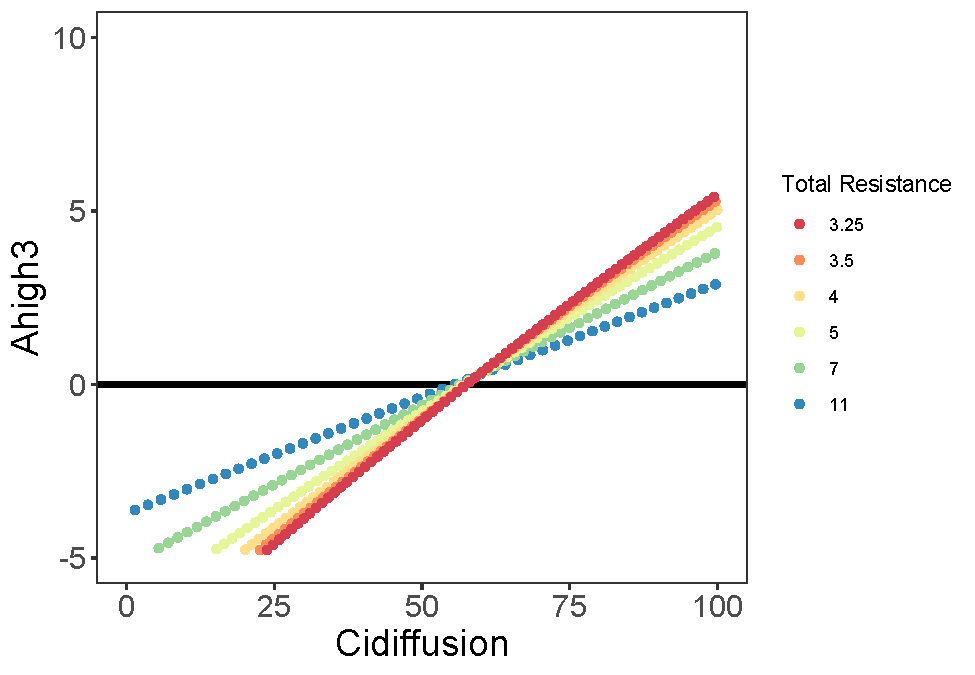
\includegraphics{bookdown_files/figure-latex/difuci-1.pdf}
\caption{\label{fig:difuci}不同 Ci 扩散限制下的差异}
\end{figure}

\begin{Shaded}
\begin{Highlighting}[]
\NormalTok{datahigh <-}\StringTok{ }\NormalTok{data[data}\OperatorTok{$}\NormalTok{resistance }\OperatorTok{==}\StringTok{ "11"}\NormalTok{,]}
\NormalTok{graph <-}\StringTok{ }\KeywordTok{ggplot}\NormalTok{(datahigh, }\KeywordTok{aes}\NormalTok{(}\DataTypeTok{x =}\NormalTok{ Cidiffusion, }\DataTypeTok{y =}\NormalTok{ Ahigh3)) }\OperatorTok{+}
\StringTok{  }\KeywordTok{geom_abline}\NormalTok{(}\DataTypeTok{slope=}\DecValTok{0}\NormalTok{,}\DataTypeTok{intercept=}\DecValTok{0}\NormalTok{,}\DataTypeTok{size=}\FloatTok{1.5}\NormalTok{)}\OperatorTok{+}
\StringTok{  }\KeywordTok{geom_point}\NormalTok{(}\DataTypeTok{colour =} \StringTok{"red"}\NormalTok{)}\OperatorTok{+}
\StringTok{  }\KeywordTok{geom_point}\NormalTok{(}\KeywordTok{aes}\NormalTok{(}\DataTypeTok{x =}\NormalTok{ Cidiffusion, }\DataTypeTok{y =}\NormalTok{ Ahigh2), }\DataTypeTok{colour =} \StringTok{"blue"}\NormalTok{)}\OperatorTok{+}
\StringTok{  }\KeywordTok{geom_point}\NormalTok{(}\KeywordTok{aes}\NormalTok{(}\DataTypeTok{x =}\NormalTok{ Cidiffusion, }\DataTypeTok{y =}\NormalTok{ Ahigh), }\DataTypeTok{colour =} \StringTok{"green"}\NormalTok{)}\OperatorTok{+}
\StringTok{  }\KeywordTok{labs}\NormalTok{(}\DataTypeTok{colour =} \StringTok{'Total Resistance'}\NormalTok{)}\OperatorTok{+}
\StringTok{  }\KeywordTok{scale_colour_brewer}\NormalTok{(}\DataTypeTok{palette =} \StringTok{'Spectral'}\NormalTok{) }\OperatorTok{+}
\StringTok{  }\KeywordTok{theme_bw}\NormalTok{() }\OperatorTok{+}
\StringTok{  }\KeywordTok{scale_x_continuous}\NormalTok{(}\DataTypeTok{limits=}\KeywordTok{c}\NormalTok{(}\DecValTok{0}\NormalTok{,}\DecValTok{100}\NormalTok{))}\OperatorTok{+}
\StringTok{  }\KeywordTok{scale_y_continuous}\NormalTok{(}\DataTypeTok{limits=}\KeywordTok{c}\NormalTok{(}\OperatorTok{-}\FloatTok{2.5}\NormalTok{,}\FloatTok{2.5}\NormalTok{))}\OperatorTok{+}
\StringTok{  }\KeywordTok{theme}\NormalTok{(}
    \DataTypeTok{axis.title =} \KeywordTok{element_text}\NormalTok{(}\DataTypeTok{size =} \DecValTok{18}\NormalTok{),}
    \DataTypeTok{axis.text =} \KeywordTok{element_text}\NormalTok{(}\DataTypeTok{size =} \DecValTok{15}\NormalTok{),}
    \DataTypeTok{legend.position =} \StringTok{'right'}\NormalTok{,}
    \DataTypeTok{panel.grid.major =} \KeywordTok{element_blank}\NormalTok{(),}
    \DataTypeTok{panel.grid.minor =} \KeywordTok{element_blank}\NormalTok{()}
\NormalTok{  )}
\NormalTok{graph}
\end{Highlighting}
\end{Shaded}

\begin{figure}
\centering
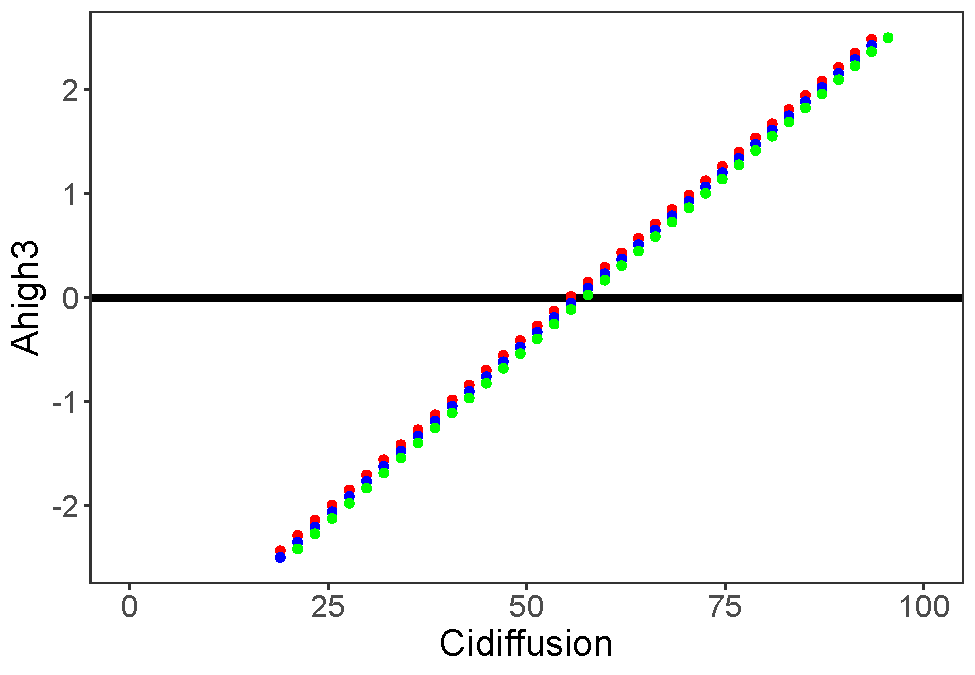
\includegraphics{bookdown_files/figure-latex/difuci11-1.pdf}
\caption{\label{fig:difuci11}不同 Ci 扩散限制下的差异(resistance = 11)}
\end{figure}

\begin{Shaded}
\begin{Highlighting}[]
\NormalTok{data2 <-}\StringTok{ }\KeywordTok{read.csv}\NormalTok{(}\StringTok{"./data/DiffusionLimits.csv"}\NormalTok{)}
\NormalTok{graph <-}\StringTok{ }\KeywordTok{ggplot}\NormalTok{(data2, }\KeywordTok{aes}\NormalTok{(}\DataTypeTok{x =}\NormalTok{ TotalRes, }\DataTypeTok{y =}\NormalTok{ Rates, }\DataTypeTok{colour =}\NormalTok{ Scenario)) }\OperatorTok{+}
\StringTok{  }\KeywordTok{geom_point}\NormalTok{()}\OperatorTok{+}
\StringTok{  }\KeywordTok{scale_colour_brewer}\NormalTok{(}\DataTypeTok{palette =} \StringTok{'Spectral'}\NormalTok{) }\OperatorTok{+}
\StringTok{  }\KeywordTok{theme_bw}\NormalTok{() }\OperatorTok{+}
\StringTok{  }\KeywordTok{theme}\NormalTok{(}
    \DataTypeTok{axis.title =} \KeywordTok{element_text}\NormalTok{(}\DataTypeTok{size =} \DecValTok{18}\NormalTok{),}
    \DataTypeTok{axis.text =} \KeywordTok{element_text}\NormalTok{(}\DataTypeTok{size =} \DecValTok{12}\NormalTok{),}
    \DataTypeTok{panel.grid.major =} \KeywordTok{element_blank}\NormalTok{(),}
    \DataTypeTok{panel.grid.minor =} \KeywordTok{element_blank}\NormalTok{()}
\NormalTok{  )}
\NormalTok{graph}
\end{Highlighting}
\end{Shaded}

\begin{figure}
\centering
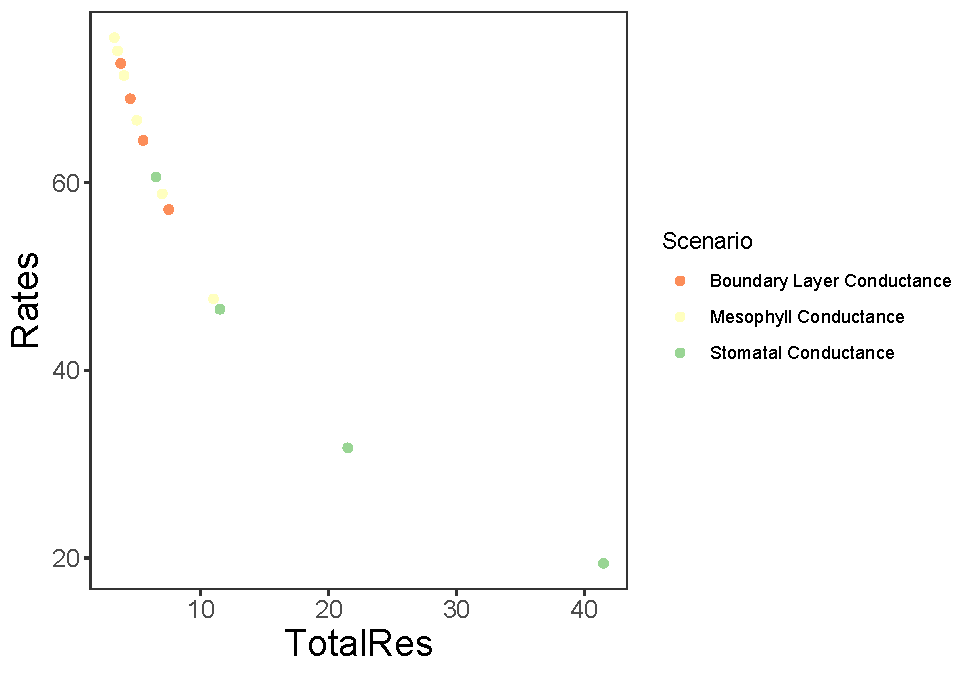
\includegraphics{bookdown_files/figure-latex/tolresis-1.pdf}
\caption{\label{fig:tolresis}不同总导度下的各个导度的速率变化}
\end{figure}

\begin{Shaded}
\begin{Highlighting}[]
\NormalTok{m1 <-}\StringTok{ }\KeywordTok{lm}\NormalTok{(Rates }\OperatorTok{~}\StringTok{ }\KeywordTok{I}\NormalTok{(}\DecValTok{1}\OperatorTok{/}\NormalTok{TotalRes)}\OperatorTok{+}\KeywordTok{I}\NormalTok{((}\DecValTok{1}\OperatorTok{/}\NormalTok{TotalRes)}\OperatorTok{^}\DecValTok{2}\NormalTok{),}\DataTypeTok{data=}\NormalTok{data2)}
\KeywordTok{summary}\NormalTok{(m1)}
\end{Highlighting}
\end{Shaded}

\begin{verbatim}
## 
## Call:
## lm(formula = Rates ~ I(1/TotalRes) + I((1/TotalRes)^2), data = data2)
## 
## Residuals:
##     Min      1Q  Median      3Q     Max 
## -3.3590 -0.9844 -0.1236  0.7706  2.4510 
## 
## Coefficients:
##                   Estimate Std. Error t value Pr(>|t|)    
## (Intercept)         13.042      1.684   7.745 3.18e-06 ***
## I(1/TotalRes)      421.928     22.487  18.763 8.49e-11 ***
## I((1/TotalRes)^2) -737.690     65.500 -11.262 4.46e-08 ***
## ---
## Signif. codes:  0 '***' 0.001 '**' 0.01 '*' 0.05 '.' 0.1 ' ' 1
## 
## Residual standard error: 1.705 on 13 degrees of freedom
## Multiple R-squared:  0.9904, Adjusted R-squared:  0.9889 
## F-statistic: 668.8 on 2 and 13 DF,  p-value: 7.799e-14
\end{verbatim}

\begin{Shaded}
\begin{Highlighting}[]
\NormalTok{ab <-}\StringTok{ }\KeywordTok{predict}\NormalTok{(m1)}
\NormalTok{red <-}\StringTok{ }\DecValTok{1}\OperatorTok{/}\NormalTok{data2}\OperatorTok{$}\NormalTok{TotalRes}
\KeywordTok{plot}\NormalTok{(ab}\OperatorTok{~}\NormalTok{red)}
\end{Highlighting}
\end{Shaded}

\begin{figure}
\centering
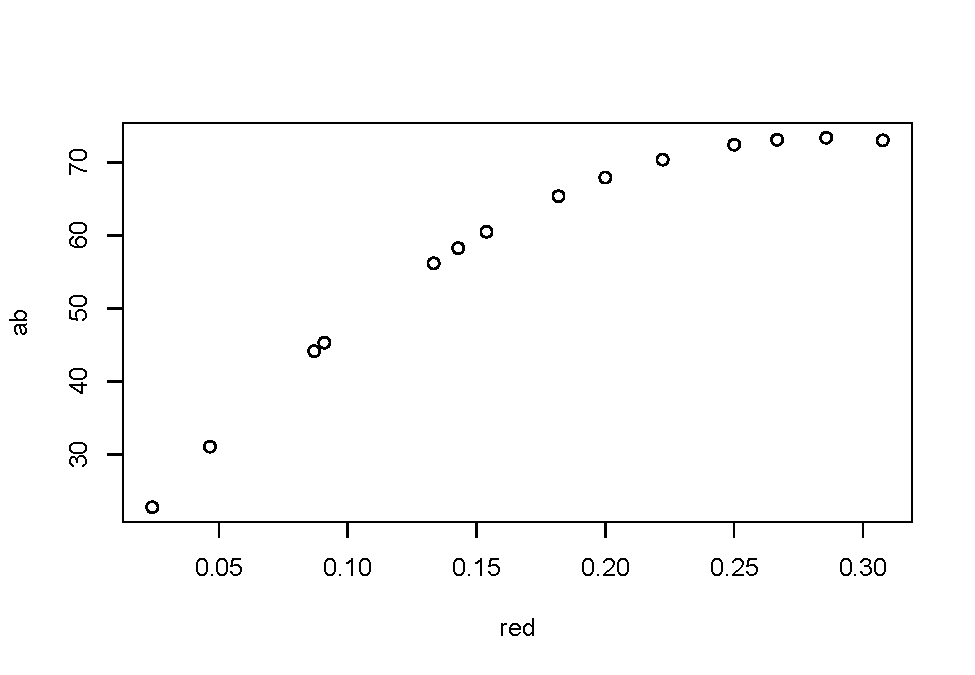
\includegraphics{bookdown_files/figure-latex/tolre-1.pdf}
\caption{\label{fig:tolre}不同阻力下的各个导度的速率变化预测值}
\end{figure}

\hypertarget{compen-estimate}{%
\subsection{补偿点的计算}\label{compen-estimate}}

计算补偿点,代码同前文类似,只是采用了不同导度下的数值:

\begin{Shaded}
\begin{Highlighting}[]
\NormalTok{data <-}\StringTok{ }\KeywordTok{read.csv}\NormalTok{(}\StringTok{"./data/DiffusionLimitsACI2.csv"}\NormalTok{)}
\CommentTok{#Gamma}
\CommentTok{# For Ci-based estimates, only use Ci < 100}
\NormalTok{dataCi <-}\StringTok{ }\NormalTok{data[data}\OperatorTok{$}\NormalTok{Cidiffusion }\OperatorTok{<}\StringTok{ }\DecValTok{100}\NormalTok{, ]}
\NormalTok{dataCi0125 <-}\StringTok{ }\NormalTok{dataCi[dataCi}\OperatorTok{$}\NormalTok{conductance }\OperatorTok{==}\StringTok{ "0.125"}\NormalTok{, ]}
\NormalTok{dataCi025 <-}\StringTok{ }\NormalTok{dataCi[dataCi}\OperatorTok{$}\NormalTok{conductance }\OperatorTok{==}\StringTok{ "0.25"}\NormalTok{, ]}
\NormalTok{dataCi05 <-}\StringTok{ }\NormalTok{dataCi[dataCi}\OperatorTok{$}\NormalTok{conductance }\OperatorTok{==}\StringTok{ "0.5"}\NormalTok{, ]}
\NormalTok{dataCi1 <-}\StringTok{ }\NormalTok{dataCi[dataCi}\OperatorTok{$}\NormalTok{conductance }\OperatorTok{==}\StringTok{ "1"}\NormalTok{, ]}
\NormalTok{dataCi2 <-}\StringTok{ }\NormalTok{dataCi[dataCi}\OperatorTok{$}\NormalTok{conductance }\OperatorTok{==}\StringTok{ "2"}\NormalTok{, ]}
\NormalTok{dataCi4 <-}\StringTok{ }\NormalTok{dataCi[dataCi}\OperatorTok{$}\NormalTok{conductance }\OperatorTok{==}\StringTok{ "4"}\NormalTok{, ]}
\NormalTok{m1 <-}\StringTok{ }\KeywordTok{lm}\NormalTok{(dataCi0125}\OperatorTok{$}\NormalTok{Ahigh }\OperatorTok{~}\StringTok{ }\NormalTok{dataCi0125}\OperatorTok{$}\NormalTok{Cidiffusion)}
\KeywordTok{summary}\NormalTok{(m1)}
\end{Highlighting}
\end{Shaded}

\begin{verbatim}
## 
## Call:
## lm(formula = dataCi0125$Ahigh ~ dataCi0125$Cidiffusion)
## 
## Residuals:
##       Min        1Q    Median        3Q       Max 
## -0.040649 -0.014495  0.005307  0.017054  0.021232 
## 
## Coefficients:
##                          Estimate Std. Error t value Pr(>|t|)    
## (Intercept)            -3.836e+00  4.318e-03  -888.5   <2e-16 ***
## dataCi0125$Cidiffusion  6.665e-02  7.873e-05   846.6   <2e-16 ***
## ---
## Signif. codes:  0 '***' 0.001 '**' 0.01 '*' 0.05 '.' 0.1 ' ' 1
## 
## Residual standard error: 0.01934 on 52 degrees of freedom
## Multiple R-squared:  0.9999, Adjusted R-squared:  0.9999 
## F-statistic: 7.167e+05 on 1 and 52 DF,  p-value: < 2.2e-16
\end{verbatim}

\begin{Shaded}
\begin{Highlighting}[]
\NormalTok{Gamma0125 <-}\StringTok{ }\OperatorTok{-}\NormalTok{m1}\OperatorTok{$}\NormalTok{coefficients[}\DecValTok{1}\NormalTok{] }\OperatorTok{/}\StringTok{ }\NormalTok{m1}\OperatorTok{$}\NormalTok{coefficients[}\DecValTok{2}\NormalTok{]}
\NormalTok{m2 <-}\StringTok{ }\KeywordTok{lm}\NormalTok{(dataCi025}\OperatorTok{$}\NormalTok{Ahigh }\OperatorTok{~}\StringTok{ }\NormalTok{dataCi025}\OperatorTok{$}\NormalTok{Cidiffusion)}
\KeywordTok{summary}\NormalTok{(m2)}
\end{Highlighting}
\end{Shaded}

\begin{verbatim}
## 
## Call:
## lm(formula = dataCi025$Ahigh ~ dataCi025$Cidiffusion)
## 
## Residuals:
##       Min        1Q    Median        3Q       Max 
## -0.070876 -0.025427  0.009071  0.029765  0.036593 
## 
## Coefficients:
##                         Estimate Std. Error t value Pr(>|t|)    
## (Intercept)           -5.2507346  0.0092187  -569.6   <2e-16 ***
## dataCi025$Cidiffusion  0.0904227  0.0001544   585.5   <2e-16 ***
## ---
## Signif. codes:  0 '***' 0.001 '**' 0.01 '*' 0.05 '.' 0.1 ' ' 1
## 
## Residual standard error: 0.03329 on 59 degrees of freedom
## Multiple R-squared:  0.9998, Adjusted R-squared:  0.9998 
## F-statistic: 3.428e+05 on 1 and 59 DF,  p-value: < 2.2e-16
\end{verbatim}

\begin{Shaded}
\begin{Highlighting}[]
\NormalTok{Gamma025 <-}\StringTok{ }\OperatorTok{-}\NormalTok{m2}\OperatorTok{$}\NormalTok{coefficients[}\DecValTok{1}\NormalTok{] }\OperatorTok{/}\StringTok{ }\NormalTok{m2}\OperatorTok{$}\NormalTok{coefficients[}\DecValTok{2}\NormalTok{]}
\NormalTok{m3 <-}\StringTok{ }\KeywordTok{lm}\NormalTok{(dataCi05}\OperatorTok{$}\NormalTok{Ahigh }\OperatorTok{~}\StringTok{ }\NormalTok{dataCi05}\OperatorTok{$}\NormalTok{Cidiffusion)}
\KeywordTok{summary}\NormalTok{(m3)}
\end{Highlighting}
\end{Shaded}

\begin{verbatim}
## 
## Call:
## lm(formula = dataCi05$Ahigh ~ dataCi05$Cidiffusion)
## 
## Residuals:
##      Min       1Q   Median       3Q      Max 
## -0.10435 -0.03583  0.01358  0.04311  0.05340 
## 
## Coefficients:
##                        Estimate Std. Error t value Pr(>|t|)    
## (Intercept)          -6.4051036  0.0150363    -426   <2e-16 ***
## dataCi05$Cidiffusion  0.1097686  0.0002391     459   <2e-16 ***
## ---
## Signif. codes:  0 '***' 0.001 '**' 0.01 '*' 0.05 '.' 0.1 ' ' 1
## 
## Residual standard error: 0.04851 on 65 degrees of freedom
## Multiple R-squared:  0.9997, Adjusted R-squared:  0.9997 
## F-statistic: 2.107e+05 on 1 and 65 DF,  p-value: < 2.2e-16
\end{verbatim}

\begin{Shaded}
\begin{Highlighting}[]
\NormalTok{Gamma05 <-}\StringTok{ }\OperatorTok{-}\NormalTok{m3}\OperatorTok{$}\NormalTok{coefficients[}\DecValTok{1}\NormalTok{] }\OperatorTok{/}\StringTok{ }\NormalTok{m3}\OperatorTok{$}\NormalTok{coefficients[}\DecValTok{2}\NormalTok{]}
\NormalTok{m4 <-}\StringTok{ }\KeywordTok{lm}\NormalTok{(dataCi1}\OperatorTok{$}\NormalTok{Ahigh }\OperatorTok{~}\StringTok{ }\NormalTok{dataCi1}\OperatorTok{$}\NormalTok{Cidiffusion)}
\KeywordTok{summary}\NormalTok{(m4)}
\end{Highlighting}
\end{Shaded}

\begin{verbatim}
## 
## Call:
## lm(formula = dataCi1$Ahigh ~ dataCi1$Cidiffusion)
## 
## Residuals:
##      Min       1Q   Median       3Q      Max 
## -0.13150 -0.04513  0.01709  0.05402  0.06692 
## 
## Coefficients:
##                       Estimate Std. Error t value Pr(>|t|)    
## (Intercept)         -7.1817472  0.0199135  -360.6   <2e-16 ***
## dataCi1$Cidiffusion  0.1227771  0.0003085   398.0   <2e-16 ***
## ---
## Signif. codes:  0 '***' 0.001 '**' 0.01 '*' 0.05 '.' 0.1 ' ' 1
## 
## Residual standard error: 0.06074 on 69 degrees of freedom
## Multiple R-squared:  0.9996, Adjusted R-squared:  0.9996 
## F-statistic: 1.584e+05 on 1 and 69 DF,  p-value: < 2.2e-16
\end{verbatim}

\begin{Shaded}
\begin{Highlighting}[]
\NormalTok{Gamma1 <-}\StringTok{ }\OperatorTok{-}\NormalTok{m4}\OperatorTok{$}\NormalTok{coefficients[}\DecValTok{1}\NormalTok{] }\OperatorTok{/}\StringTok{ }\NormalTok{m4}\OperatorTok{$}\NormalTok{coefficients[}\DecValTok{2}\NormalTok{]}
\NormalTok{m5 <-}\StringTok{ }\KeywordTok{lm}\NormalTok{(dataCi2}\OperatorTok{$}\NormalTok{Ahigh }\OperatorTok{~}\StringTok{ }\NormalTok{dataCi2}\OperatorTok{$}\NormalTok{Cidiffusion)}
\KeywordTok{summary}\NormalTok{(m5)}
\end{Highlighting}
\end{Shaded}

\begin{verbatim}
## 
## Call:
## lm(formula = dataCi2$Ahigh ~ dataCi2$Cidiffusion)
## 
## Residuals:
##      Min       1Q   Median       3Q      Max 
## -0.14803 -0.04874  0.01837  0.05995  0.07511 
## 
## Coefficients:
##                       Estimate Std. Error t value Pr(>|t|)    
## (Intercept)         -7.6427727  0.0230595  -331.4   <2e-16 ***
## dataCi2$Cidiffusion  0.1305083  0.0003538   368.9   <2e-16 ***
## ---
## Signif. codes:  0 '***' 0.001 '**' 0.01 '*' 0.05 '.' 0.1 ' ' 1
## 
## Residual standard error: 0.06815 on 71 degrees of freedom
## Multiple R-squared:  0.9995, Adjusted R-squared:  0.9995 
## F-statistic: 1.361e+05 on 1 and 71 DF,  p-value: < 2.2e-16
\end{verbatim}

\begin{Shaded}
\begin{Highlighting}[]
\NormalTok{Gamma2 <-}\StringTok{ }\OperatorTok{-}\NormalTok{m5}\OperatorTok{$}\NormalTok{coefficients[}\DecValTok{1}\NormalTok{] }\OperatorTok{/}\StringTok{ }\NormalTok{m5}\OperatorTok{$}\NormalTok{coefficients[}\DecValTok{2}\NormalTok{]}
\NormalTok{m6 <-}\StringTok{ }\KeywordTok{lm}\NormalTok{(dataCi4}\OperatorTok{$}\NormalTok{Ahigh }\OperatorTok{~}\StringTok{ }\NormalTok{dataCi4}\OperatorTok{$}\NormalTok{Cidiffusion)}
\KeywordTok{summary}\NormalTok{(m6)}
\end{Highlighting}
\end{Shaded}

\begin{verbatim}
## 
## Call:
## lm(formula = dataCi4$Ahigh ~ dataCi4$Cidiffusion)
## 
## Residuals:
##      Min       1Q   Median       3Q      Max 
## -0.15721 -0.05258  0.01994  0.06470  0.07968 
## 
## Coefficients:
##                       Estimate Std. Error t value Pr(>|t|)    
## (Intercept)         -7.8955772  0.0248634  -317.6   <2e-16 ***
## dataCi4$Cidiffusion  0.1347503  0.0003799   354.7   <2e-16 ***
## ---
## Signif. codes:  0 '***' 0.001 '**' 0.01 '*' 0.05 '.' 0.1 ' ' 1
## 
## Residual standard error: 0.07225 on 72 degrees of freedom
## Multiple R-squared:  0.9994, Adjusted R-squared:  0.9994 
## F-statistic: 1.258e+05 on 1 and 72 DF,  p-value: < 2.2e-16
\end{verbatim}

\begin{Shaded}
\begin{Highlighting}[]
\NormalTok{Gamma4 <-}\StringTok{ }\OperatorTok{-}\NormalTok{m6}\OperatorTok{$}\NormalTok{coefficients[}\DecValTok{1}\NormalTok{] }\OperatorTok{/}\StringTok{ }\NormalTok{m6}\OperatorTok{$}\NormalTok{coefficients[}\DecValTok{2}\NormalTok{]}

\NormalTok{GammaCi <-}\StringTok{ }\KeywordTok{c}\NormalTok{(Gamma0125, Gamma025, Gamma05, Gamma1, Gamma2, Gamma4)}
\end{Highlighting}
\end{Shaded}

\hypertarget{all-fig}{%
\subsection{所有图形代码}\label{all-fig}}

\begin{Shaded}
\begin{Highlighting}[]
\NormalTok{data <-}\StringTok{ }\KeywordTok{read.csv}\NormalTok{(}\StringTok{"./data/PRdata.csv"}\NormalTok{)}
\NormalTok{data}\OperatorTok{$}\NormalTok{Ccfull <-}\StringTok{ }\KeywordTok{as.numeric}\NormalTok{(data}\OperatorTok{$}\NormalTok{Ccfull)}
\NormalTok{data}\OperatorTok{$}\NormalTok{Delay <-}\StringTok{ }\KeywordTok{as.factor}\NormalTok{(data}\OperatorTok{$}\NormalTok{Delay)}
\NormalTok{cols <-}\StringTok{ }\KeywordTok{gg_color_hue}\NormalTok{(}\DecValTok{6}\NormalTok{)}
\NormalTok{Panel_1A <-}
\StringTok{  }\KeywordTok{ggplot}\NormalTok{(data, }\KeywordTok{aes}\NormalTok{(}
    \DataTypeTok{x =}\NormalTok{ Cifull,}
    \DataTypeTok{y =}\NormalTok{ Anet,}
    \DataTypeTok{colour =}\NormalTok{ Delay,}
    \DataTypeTok{linetype =}\NormalTok{ Delay}
\NormalTok{  )) }\OperatorTok{+}
\StringTok{  }\CommentTok{# 零水平参考线}
\StringTok{  }\KeywordTok{geom_abline}\NormalTok{(}\DataTypeTok{slope =} \DecValTok{0}\NormalTok{,}
              \DataTypeTok{intercept =} \DecValTok{0}\NormalTok{,}
              \DataTypeTok{size =} \FloatTok{1.5}\NormalTok{) }\OperatorTok{+}
\StringTok{  }\CommentTok{#ci与A loess 方法的拟合曲线}
\StringTok{  }\KeywordTok{geom_smooth}\NormalTok{(}\DataTypeTok{method =} \StringTok{"loess"}\NormalTok{, }\DataTypeTok{se =} \OtherTok{FALSE}\NormalTok{, }\DataTypeTok{size =} \DecValTok{2}\NormalTok{) }\OperatorTok{+}
\StringTok{  }\KeywordTok{scale_linetype_manual}\NormalTok{(}
    \DataTypeTok{name =} \StringTok{"Delay (s)"}\NormalTok{,}
    \DataTypeTok{labels =} \KeywordTok{c}\NormalTok{(}\StringTok{"0"}\NormalTok{, }\StringTok{"15"}\NormalTok{, }\StringTok{"30"}\NormalTok{, }\StringTok{"60"}\NormalTok{, }\StringTok{"120"}\NormalTok{, }\StringTok{"300"}\NormalTok{),}
    \DataTypeTok{values =} \KeywordTok{c}\NormalTok{(}\StringTok{"solid"}\NormalTok{, }\StringTok{"longdash"}\NormalTok{, }\StringTok{"twodash"}\NormalTok{, }\StringTok{"dotdash"}\NormalTok{, }\StringTok{"dashed"}\NormalTok{, }\StringTok{"dotted"}\NormalTok{)}
\NormalTok{  ) }\OperatorTok{+}
\StringTok{  }\KeywordTok{ggtitle}\NormalTok{(}\KeywordTok{expression}\NormalTok{(}\KeywordTok{paste}\NormalTok{(}
    \KeywordTok{bold}\NormalTok{(}\StringTok{"(a)"}\NormalTok{), }\StringTok{" Modelled Photorespiratory Effect"}
\NormalTok{  ))) }\OperatorTok{+}
\StringTok{  }\KeywordTok{labs}\NormalTok{(}\DataTypeTok{x =} \KeywordTok{expression}\NormalTok{(C[i] }\OperatorTok{~}\StringTok{ "("} \OperatorTok{*}\StringTok{ }\NormalTok{mu }\OperatorTok{*}\StringTok{ }\NormalTok{mol }\OperatorTok{~}\StringTok{ }\NormalTok{mol }\OperatorTok{^}\StringTok{ }\NormalTok{\{}
    \DecValTok{-1}
\NormalTok{  \} }\OperatorTok{*}\StringTok{ ")"}\NormalTok{),}
  \DataTypeTok{y =} \KeywordTok{expression}\NormalTok{(A[net] }\OperatorTok{~}\StringTok{ "("} \OperatorTok{*}\StringTok{ }\NormalTok{mu }\OperatorTok{*}\StringTok{ }\NormalTok{mol }\OperatorTok{~}\StringTok{ }\NormalTok{m }\OperatorTok{^}\StringTok{ }\NormalTok{\{}
    \DecValTok{-2}
\NormalTok{  \} }\OperatorTok{~}\StringTok{ }\NormalTok{s }\OperatorTok{^}\StringTok{ }\NormalTok{\{}
    \DecValTok{-1}
\NormalTok{  \} }\OperatorTok{*}\StringTok{ ")"}\NormalTok{)) }\OperatorTok{+}
\StringTok{  }\KeywordTok{labs}\NormalTok{(}\DataTypeTok{colour =} \StringTok{'Delay (s)'}\NormalTok{) }\OperatorTok{+}
\StringTok{  }\KeywordTok{scale_x_continuous}\NormalTok{(}\DataTypeTok{limits =} \KeywordTok{c}\NormalTok{(}\DecValTok{0}\NormalTok{, }\DecValTok{250}\NormalTok{)) }\OperatorTok{+}
\StringTok{  }\KeywordTok{scale_y_continuous}\NormalTok{(}\DataTypeTok{limits =} \KeywordTok{c}\NormalTok{(}\OperatorTok{-}\DecValTok{5}\NormalTok{, }\DecValTok{20}\NormalTok{)) }\OperatorTok{+}
\StringTok{  }\KeywordTok{scale_colour_manual}\NormalTok{(}
    \DataTypeTok{values =}\NormalTok{ cols,}
    \DataTypeTok{name =} \StringTok{"Delay (s)"}\NormalTok{,}
    \DataTypeTok{labels =} \KeywordTok{c}\NormalTok{(}\StringTok{"0"}\NormalTok{, }\StringTok{"15"}\NormalTok{, }\StringTok{"30"}\NormalTok{, }\StringTok{"60"}\NormalTok{, }\StringTok{"120"}\NormalTok{, }\StringTok{"300"}\NormalTok{)}
\NormalTok{  ) }\OperatorTok{+}
\StringTok{  }\KeywordTok{theme_bw}\NormalTok{() }\OperatorTok{+}
\StringTok{  }\KeywordTok{theme}\NormalTok{(}
    \DataTypeTok{axis.title.x =} \KeywordTok{element_text}\NormalTok{(}\DataTypeTok{size =} \DecValTok{20}\NormalTok{),}
    \DataTypeTok{axis.title.y =} \KeywordTok{element_text}\NormalTok{(}\DataTypeTok{size =} \DecValTok{20}\NormalTok{),}
    \DataTypeTok{axis.line =} \KeywordTok{element_line}\NormalTok{(}\DataTypeTok{size =} \DecValTok{1}\NormalTok{),}
    \DataTypeTok{axis.ticks =} \KeywordTok{element_line}\NormalTok{(}\DataTypeTok{size =} \FloatTok{1.5}\NormalTok{),}
    \DataTypeTok{axis.ticks.length =} \KeywordTok{unit}\NormalTok{(}\FloatTok{1.5}\NormalTok{, }\StringTok{"mm"}\NormalTok{),}
    \DataTypeTok{rect =} \KeywordTok{element_rect}\NormalTok{(}\DataTypeTok{size =} \DecValTok{2}\NormalTok{),}
    \DataTypeTok{axis.text.x =} \KeywordTok{element_text}\NormalTok{(}\DataTypeTok{size =} \DecValTok{14}\NormalTok{, }\DataTypeTok{color =} \StringTok{'black'}\NormalTok{),}
    \DataTypeTok{axis.text.y =}
      \KeywordTok{element_text}\NormalTok{(}
        \DataTypeTok{size =} \DecValTok{14}\NormalTok{,}
        \DataTypeTok{color =} \StringTok{'black'}\NormalTok{,}
        \DataTypeTok{hjust =}\NormalTok{ (}\DecValTok{1}\NormalTok{)}
\NormalTok{      ),}
    \DataTypeTok{legend.position =} \KeywordTok{c}\NormalTok{(}\FloatTok{0.15}\NormalTok{, }\FloatTok{0.75}\NormalTok{),}
    \DataTypeTok{axis.title =} \KeywordTok{element_text}\NormalTok{(}\DataTypeTok{size =} \DecValTok{18}\NormalTok{),}
    \DataTypeTok{axis.text =} \KeywordTok{element_text}\NormalTok{(}\DataTypeTok{size =} \DecValTok{12}\NormalTok{, }\DataTypeTok{color =} \StringTok{"black"}\NormalTok{),}
    \DataTypeTok{panel.grid.major =} \KeywordTok{element_blank}\NormalTok{(),}
    \DataTypeTok{panel.grid.minor =} \KeywordTok{element_blank}\NormalTok{(),}
    \DataTypeTok{legend.text =} \KeywordTok{element_text}\NormalTok{(}\DataTypeTok{size =} \DecValTok{14}\NormalTok{),}
    \DataTypeTok{legend.title =} \KeywordTok{element_text}\NormalTok{(}\DataTypeTok{size =} \DecValTok{14}\NormalTok{)}
\NormalTok{  )}
\NormalTok{Panel_1A}
\end{Highlighting}
\end{Shaded}

\begin{figure}
\centering
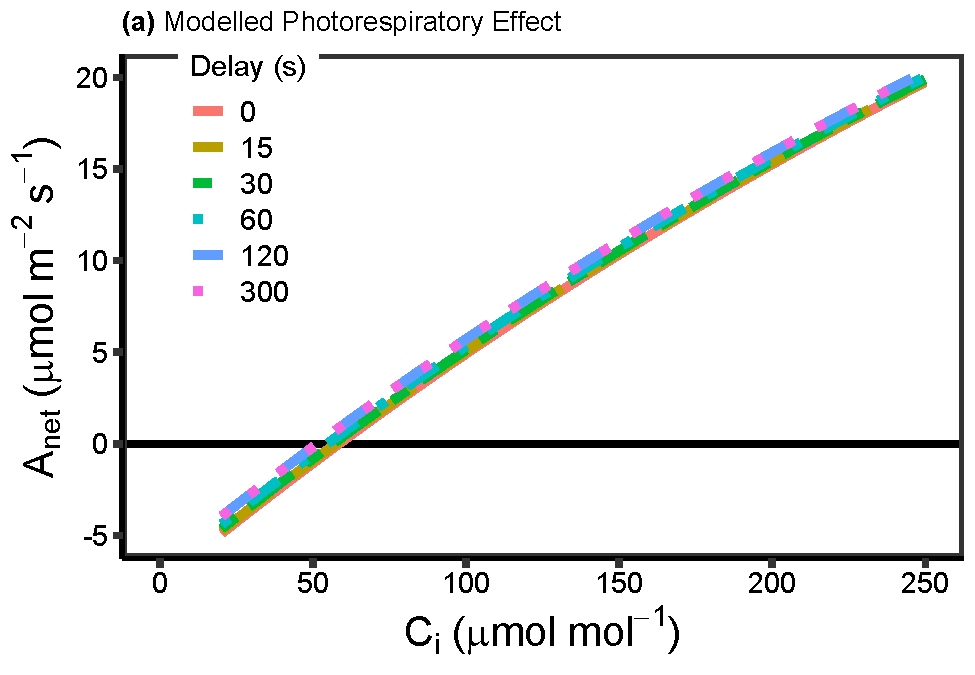
\includegraphics{bookdown_files/figure-latex/prdataplot-1.pdf}
\caption{\label{fig:prdataplot}不同时间滞后性的 Anet VS Ci}
\end{figure}

\begin{Shaded}
\begin{Highlighting}[]
\NormalTok{Panel_1A_inset <-}
\StringTok{  }\KeywordTok{ggplot}\NormalTok{(data, }\KeywordTok{aes}\NormalTok{(}
    \DataTypeTok{x =}\NormalTok{ Cifull,}
    \DataTypeTok{y =}\NormalTok{ Anet,}
    \DataTypeTok{colour =}\NormalTok{ Delay,}
    \DataTypeTok{linetype =}\NormalTok{ Delay}
\NormalTok{  )) }\OperatorTok{+}
\StringTok{  }\KeywordTok{geom_abline}\NormalTok{(}\DataTypeTok{slope =} \DecValTok{0}\NormalTok{,}
              \DataTypeTok{intercept =} \DecValTok{0}\NormalTok{,}
              \DataTypeTok{size =} \FloatTok{1.5}\NormalTok{) }\OperatorTok{+}
\StringTok{  }\KeywordTok{geom_smooth}\NormalTok{(}\DataTypeTok{method =} \StringTok{"loess"}\NormalTok{, }\DataTypeTok{se =} \OtherTok{FALSE}\NormalTok{, }\DataTypeTok{size =} \DecValTok{2}\NormalTok{) }\OperatorTok{+}
\StringTok{  }\KeywordTok{scale_linetype_manual}\NormalTok{(}
    \DataTypeTok{name =} \StringTok{"Delay (s)"}\NormalTok{,}
    \DataTypeTok{labels =} \KeywordTok{c}\NormalTok{(}\StringTok{"0"}\NormalTok{, }\StringTok{"15"}\NormalTok{, }\StringTok{"30"}\NormalTok{, }\StringTok{"60"}\NormalTok{, }\StringTok{"120"}\NormalTok{, }\StringTok{"300"}\NormalTok{),}
    \DataTypeTok{values =} \KeywordTok{c}\NormalTok{(}\StringTok{"solid"}\NormalTok{, }\StringTok{"longdash"}\NormalTok{, }\StringTok{"twodash"}\NormalTok{, }\StringTok{"dotdash"}\NormalTok{, }\StringTok{"dashed"}\NormalTok{, }\StringTok{"dotted"}\NormalTok{)}
\NormalTok{  ) }\OperatorTok{+}
\StringTok{  }\KeywordTok{labs}\NormalTok{(}\DataTypeTok{x =} \KeywordTok{expression}\NormalTok{(C[i] }\OperatorTok{~}\StringTok{ "("} \OperatorTok{*}\StringTok{ }\NormalTok{mu }\OperatorTok{*}\StringTok{ }\NormalTok{mol }\OperatorTok{~}\StringTok{ }\NormalTok{mol }\OperatorTok{^}\StringTok{ }\NormalTok{\{}
    \DecValTok{-1}
\NormalTok{  \} }\OperatorTok{*}\StringTok{ ")"}\NormalTok{),}
  \DataTypeTok{y =} \KeywordTok{expression}\NormalTok{(A[net] }\OperatorTok{~}\StringTok{ "("} \OperatorTok{*}\StringTok{ }\NormalTok{mu }\OperatorTok{*}\StringTok{ }\NormalTok{mol }\OperatorTok{~}\StringTok{ }\NormalTok{m }\OperatorTok{^}\StringTok{ }\NormalTok{\{}
    \DecValTok{-2}
\NormalTok{  \} }\OperatorTok{~}\StringTok{ }\NormalTok{s }\OperatorTok{^}\StringTok{ }\NormalTok{\{}
    \DecValTok{-1}
\NormalTok{  \} }\OperatorTok{*}\StringTok{ ")"}\NormalTok{)) }\OperatorTok{+}
\StringTok{  }\KeywordTok{labs}\NormalTok{(}\DataTypeTok{colour =} \StringTok{'Delay (s)'}\NormalTok{) }\OperatorTok{+}
\StringTok{  }\KeywordTok{scale_x_continuous}\NormalTok{(}\DataTypeTok{limits =} \KeywordTok{c}\NormalTok{(}\DecValTok{45}\NormalTok{, }\DecValTok{65}\NormalTok{)) }\OperatorTok{+}
\StringTok{  }\KeywordTok{scale_y_continuous}\NormalTok{(}\DataTypeTok{limits =} \KeywordTok{c}\NormalTok{(}\OperatorTok{-}\DecValTok{1}\NormalTok{, }\DecValTok{1}\NormalTok{), }\DataTypeTok{breaks =} \KeywordTok{c}\NormalTok{(}\OperatorTok{-}\DecValTok{1}\NormalTok{, }\DecValTok{0}\NormalTok{, }\DecValTok{1}\NormalTok{)) }\OperatorTok{+}
\StringTok{  }\KeywordTok{scale_colour_manual}\NormalTok{(}\DataTypeTok{values =}\NormalTok{ cols) }\OperatorTok{+}
\StringTok{  }\KeywordTok{theme_bw}\NormalTok{() }\OperatorTok{+}
\StringTok{  }\KeywordTok{theme}\NormalTok{(}
    \DataTypeTok{axis.title.x =} \KeywordTok{element_blank}\NormalTok{(),}
    \DataTypeTok{axis.title.y =} \KeywordTok{element_blank}\NormalTok{(),}
    \DataTypeTok{axis.line =} \KeywordTok{element_line}\NormalTok{(}\DataTypeTok{size =} \DecValTok{1}\NormalTok{),}
    \DataTypeTok{axis.ticks =} \KeywordTok{element_line}\NormalTok{(}\DataTypeTok{size =} \FloatTok{1.5}\NormalTok{),}
    \DataTypeTok{axis.ticks.length =} \KeywordTok{unit}\NormalTok{(}\FloatTok{1.5}\NormalTok{, }\StringTok{"mm"}\NormalTok{),}
    \DataTypeTok{rect =} \KeywordTok{element_rect}\NormalTok{(}\DataTypeTok{size =} \DecValTok{2}\NormalTok{),}
    \DataTypeTok{axis.text.x =} \KeywordTok{element_text}\NormalTok{(}\DataTypeTok{size =} \DecValTok{14}\NormalTok{, }\DataTypeTok{color =} \StringTok{'black'}\NormalTok{),}
    \DataTypeTok{axis.text.y =}
      \KeywordTok{element_text}\NormalTok{(}
        \DataTypeTok{size =} \DecValTok{14}\NormalTok{,}
        \DataTypeTok{color =} \StringTok{'black'}\NormalTok{,}
        \DataTypeTok{hjust =}\NormalTok{ (}\DecValTok{1}\NormalTok{)}
\NormalTok{      ),}
    \DataTypeTok{axis.title =} \KeywordTok{element_blank}\NormalTok{(),}
    \DataTypeTok{axis.text =} \KeywordTok{element_text}\NormalTok{(}\DataTypeTok{size =} \DecValTok{12}\NormalTok{, }\DataTypeTok{color =} \StringTok{"black"}\NormalTok{),}
    \DataTypeTok{panel.grid.major =} \KeywordTok{element_blank}\NormalTok{(),}
    \DataTypeTok{panel.grid.minor =} \KeywordTok{element_blank}\NormalTok{(),}
    \DataTypeTok{legend.position =} \StringTok{'none'}\NormalTok{,}
    \DataTypeTok{plot.background =} \KeywordTok{element_blank}\NormalTok{()}
\NormalTok{  )}



\NormalTok{cols <-}\StringTok{ }\KeywordTok{gg_color_hue}\NormalTok{(}\DecValTok{6}\NormalTok{)}

\NormalTok{data <-}\StringTok{ }\KeywordTok{read.csv}\NormalTok{(}\StringTok{"./data/DiffusionLimitsACI2.csv"}\NormalTok{)}
\NormalTok{data}\OperatorTok{$}\NormalTok{resistance <-}\StringTok{ }\KeywordTok{as.factor}\NormalTok{(data}\OperatorTok{$}\NormalTok{resistance)}
\NormalTok{Panel_1Db <-}
\StringTok{  }\KeywordTok{ggplot}\NormalTok{(data,}
         \KeywordTok{aes}\NormalTok{(}
           \DataTypeTok{x =}\NormalTok{ Cidiffusion,}
           \DataTypeTok{y =}\NormalTok{ Ahigh,}
           \DataTypeTok{colour =}\NormalTok{ resistance,}
           \DataTypeTok{linetype =}\NormalTok{ resistance}
\NormalTok{         )) }\OperatorTok{+}
\StringTok{  }\KeywordTok{geom_abline}\NormalTok{(}\DataTypeTok{slope =} \DecValTok{0}\NormalTok{,}
              \DataTypeTok{intercept =} \DecValTok{0}\NormalTok{,}
              \DataTypeTok{size =} \FloatTok{1.5}\NormalTok{) }\OperatorTok{+}
\StringTok{  }\KeywordTok{geom_smooth}\NormalTok{(}\DataTypeTok{method =} \StringTok{"loess"}\NormalTok{, }\DataTypeTok{se =} \OtherTok{FALSE}\NormalTok{, }\DataTypeTok{size =} \DecValTok{2}\NormalTok{) }\OperatorTok{+}
\StringTok{  }\KeywordTok{scale_linetype_manual}\NormalTok{(}
    \DataTypeTok{name =} \StringTok{"Total Resistance"}\NormalTok{,}
    \DataTypeTok{labels =} \KeywordTok{c}\NormalTok{(}\StringTok{"3.25"}\NormalTok{, }\StringTok{"3.5"}\NormalTok{, }\StringTok{"4"}\NormalTok{, }\StringTok{"5"}\NormalTok{, }\StringTok{"7"}\NormalTok{, }\StringTok{"11"}\NormalTok{),}
    \DataTypeTok{values =} \KeywordTok{c}\NormalTok{(}\StringTok{"solid"}\NormalTok{, }\StringTok{"longdash"}\NormalTok{, }\StringTok{"twodash"}\NormalTok{, }\StringTok{"dotdash"}\NormalTok{, }\StringTok{"dashed"}\NormalTok{, }\StringTok{"dotted"}\NormalTok{)}
\NormalTok{  ) }\OperatorTok{+}
\StringTok{  }\KeywordTok{ggtitle}\NormalTok{(}\KeywordTok{expression}\NormalTok{(}\KeywordTok{paste}\NormalTok{(}\KeywordTok{bold}\NormalTok{(}\StringTok{"(d)"}\NormalTok{), }\StringTok{" Modelled Resistance Effect"}\NormalTok{))) }\OperatorTok{+}
\StringTok{  }\KeywordTok{scale_color_manual}\NormalTok{(}
    \DataTypeTok{values =}\NormalTok{ cols,}
    \DataTypeTok{name =} \StringTok{"Total Resistance"}\NormalTok{,}
    \DataTypeTok{labels =} \KeywordTok{c}\NormalTok{(}\StringTok{"3.25"}\NormalTok{, }\StringTok{"3.5"}\NormalTok{, }\StringTok{"4"}\NormalTok{, }\StringTok{"5"}\NormalTok{, }\StringTok{"7"}\NormalTok{, }\StringTok{"11"}\NormalTok{)}
\NormalTok{  ) }\OperatorTok{+}
\StringTok{  }\KeywordTok{theme_bw}\NormalTok{() }\OperatorTok{+}
\StringTok{  }\KeywordTok{labs}\NormalTok{(}\DataTypeTok{x =} \KeywordTok{expression}\NormalTok{(}\KeywordTok{paste}\NormalTok{(C[i] }\OperatorTok{~}\StringTok{ "("} \OperatorTok{*}\StringTok{ }\NormalTok{mu }\OperatorTok{*}\StringTok{ }\NormalTok{mol }\OperatorTok{~}\StringTok{ }\NormalTok{mol }\OperatorTok{^}\StringTok{ }\NormalTok{\{}
    \DecValTok{-1}
\NormalTok{  \} }\OperatorTok{*}\StringTok{ ")"}\NormalTok{)), }\DataTypeTok{y =} \KeywordTok{expression}\NormalTok{(}\KeywordTok{paste}\NormalTok{(A[net] }\OperatorTok{~}\StringTok{ "("} \OperatorTok{*}\StringTok{ }\NormalTok{mu }\OperatorTok{*}\StringTok{ }\NormalTok{mol }\OperatorTok{~}\StringTok{ }\NormalTok{m }\OperatorTok{^}\StringTok{ }\NormalTok{\{}
    \DecValTok{-2}
\NormalTok{  \} }\OperatorTok{~}\StringTok{ }\NormalTok{s }\OperatorTok{^}\StringTok{ }\NormalTok{\{}
    \DecValTok{-1}
\NormalTok{  \} }\OperatorTok{*}\StringTok{ ")"}\NormalTok{))) }\OperatorTok{+}
\StringTok{  }\KeywordTok{scale_x_continuous}\NormalTok{(}\DataTypeTok{limits =} \KeywordTok{c}\NormalTok{(}\DecValTok{0}\NormalTok{, }\DecValTok{250}\NormalTok{)) }\OperatorTok{+}
\StringTok{  }\KeywordTok{scale_y_continuous}\NormalTok{(}\DataTypeTok{limits =} \KeywordTok{c}\NormalTok{(}\OperatorTok{-}\DecValTok{5}\NormalTok{, }\DecValTok{20}\NormalTok{)) }\OperatorTok{+}
\StringTok{  }\KeywordTok{theme}\NormalTok{(}
    \DataTypeTok{axis.title.x =} \KeywordTok{element_text}\NormalTok{(}\DataTypeTok{size =} \DecValTok{20}\NormalTok{),}
    \DataTypeTok{axis.title.y =} \KeywordTok{element_text}\NormalTok{(}\DataTypeTok{size =} \DecValTok{20}\NormalTok{),}
    \DataTypeTok{axis.line =} \KeywordTok{element_line}\NormalTok{(}\DataTypeTok{size =} \DecValTok{1}\NormalTok{),}
    \DataTypeTok{axis.ticks =} \KeywordTok{element_line}\NormalTok{(}\DataTypeTok{size =} \FloatTok{1.5}\NormalTok{),}
    \DataTypeTok{axis.ticks.length =} \KeywordTok{unit}\NormalTok{(}\FloatTok{1.5}\NormalTok{, }\StringTok{"mm"}\NormalTok{),}
    \DataTypeTok{rect =} \KeywordTok{element_rect}\NormalTok{(}\DataTypeTok{size =} \DecValTok{2}\NormalTok{),}
    \DataTypeTok{axis.text.x =} \KeywordTok{element_text}\NormalTok{(}\DataTypeTok{size =} \DecValTok{14}\NormalTok{, }\DataTypeTok{color =} \StringTok{'black'}\NormalTok{),}
    \DataTypeTok{axis.text.y =}
      \KeywordTok{element_text}\NormalTok{(}
        \DataTypeTok{size =} \DecValTok{14}\NormalTok{,}
        \DataTypeTok{color =} \StringTok{'black'}\NormalTok{,}
        \DataTypeTok{hjust =}\NormalTok{ (}\DecValTok{1}\NormalTok{)}
\NormalTok{      ),}
    \DataTypeTok{legend.position =} \KeywordTok{c}\NormalTok{(}\FloatTok{0.22}\NormalTok{, }\FloatTok{0.75}\NormalTok{),}
    \DataTypeTok{axis.title =} \KeywordTok{element_text}\NormalTok{(}\DataTypeTok{size =} \DecValTok{18}\NormalTok{),}
    \DataTypeTok{axis.text =} \KeywordTok{element_text}\NormalTok{(}\DataTypeTok{size =} \DecValTok{12}\NormalTok{, }\DataTypeTok{color =} \StringTok{"black"}\NormalTok{),}
    \DataTypeTok{panel.grid.major =} \KeywordTok{element_blank}\NormalTok{(),}
    \DataTypeTok{panel.grid.minor =} \KeywordTok{element_blank}\NormalTok{(),}
    \DataTypeTok{legend.text =} \KeywordTok{element_text}\NormalTok{(}\DataTypeTok{size =} \DecValTok{14}\NormalTok{),}
    \DataTypeTok{legend.title =} \KeywordTok{element_text}\NormalTok{(}\DataTypeTok{size =} \DecValTok{14}\NormalTok{)}
\NormalTok{  )}
\NormalTok{Panel_1Db}
\end{Highlighting}
\end{Shaded}

\begin{figure}
\centering
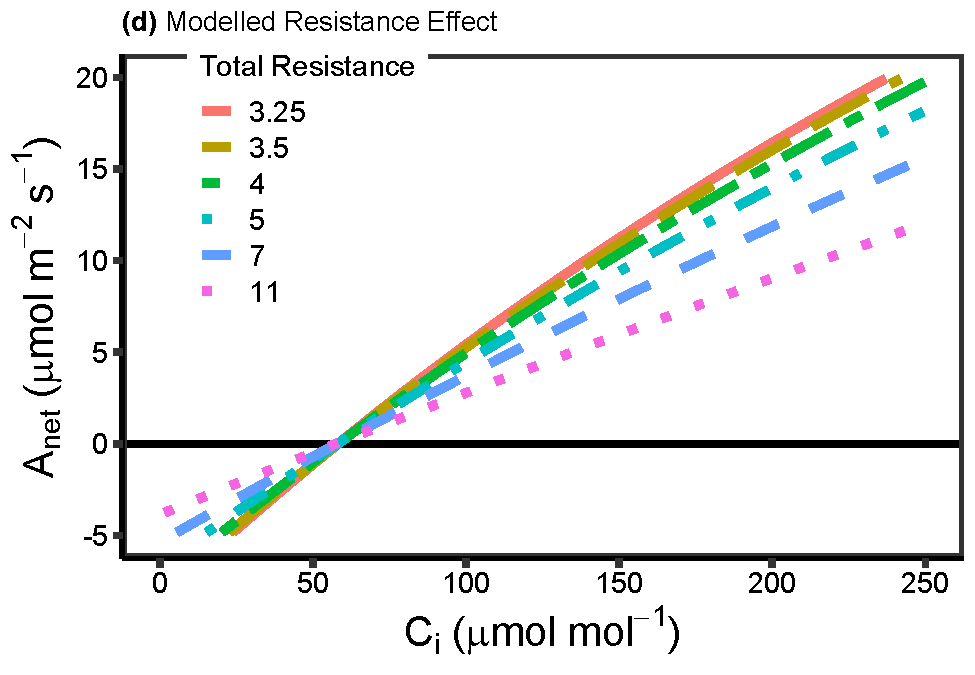
\includegraphics{bookdown_files/figure-latex/resistplot-1.pdf}
\caption{\label{fig:resistplot}不同总阻力下的 Anet VS Ci}
\end{figure}

\begin{Shaded}
\begin{Highlighting}[]
\NormalTok{data <-}\StringTok{ }\KeywordTok{read.csv}\NormalTok{(}\StringTok{"./data/DiffusionLimitsACI2.csv"}\NormalTok{)}
\NormalTok{data}\OperatorTok{$}\NormalTok{resistance <-}\StringTok{ }\KeywordTok{as.factor}\NormalTok{(data}\OperatorTok{$}\NormalTok{resistance)}
\NormalTok{data <-}\StringTok{ }\NormalTok{data[data}\OperatorTok{$}\NormalTok{resistance }\OperatorTok{==}\StringTok{ "11"}\NormalTok{,]}
\NormalTok{resistance <-}\StringTok{ }\KeywordTok{rep}\NormalTok{(data}\OperatorTok{$}\NormalTok{resistance, }\DecValTok{3}\NormalTok{)}
\NormalTok{Cidiffusion <-}\StringTok{ }\KeywordTok{rep}\NormalTok{(data}\OperatorTok{$}\NormalTok{Cidffusion, }\DecValTok{3}\NormalTok{)}
\NormalTok{A <-}\StringTok{ }\KeywordTok{c}\NormalTok{(data}\OperatorTok{$}\NormalTok{Ahigh, data}\OperatorTok{$}\NormalTok{Ahigh2, data}\OperatorTok{$}\NormalTok{Ahigh3)}
\NormalTok{Rate <-}
\StringTok{  }\KeywordTok{c}\NormalTok{(}\KeywordTok{rep}\NormalTok{(}\DecValTok{100}\NormalTok{, }\KeywordTok{length}\NormalTok{(data}\OperatorTok{$}\NormalTok{Ahigh)), }\KeywordTok{rep}\NormalTok{(}\DecValTok{200}\NormalTok{, }\KeywordTok{length}\NormalTok{(data}\OperatorTok{$}\NormalTok{Ahigh2)), }\KeywordTok{rep}\NormalTok{(}\DecValTok{300}\NormalTok{, }\KeywordTok{length}\NormalTok{(data}\OperatorTok{$}\NormalTok{Ahigh3)))}
\NormalTok{data3 <-}\StringTok{ }\KeywordTok{rbind}\NormalTok{(data, data, data)}
\NormalTok{data3}\OperatorTok{$}\NormalTok{A <-}\StringTok{ }\KeywordTok{c}\NormalTok{(data}\OperatorTok{$}\NormalTok{Ahigh, data}\OperatorTok{$}\NormalTok{Ahigh2, data}\OperatorTok{$}\NormalTok{Ahigh3)}
\NormalTok{data3}\OperatorTok{$}\NormalTok{Rate <-}
\StringTok{  }\KeywordTok{as.factor}\NormalTok{(}\KeywordTok{c}\NormalTok{(}\KeywordTok{rep}\NormalTok{(}\DecValTok{100}\NormalTok{, }\KeywordTok{length}\NormalTok{(data}\OperatorTok{$}\NormalTok{Ahigh)), }\KeywordTok{rep}\NormalTok{(}\DecValTok{200}\NormalTok{, }\KeywordTok{length}\NormalTok{(data}\OperatorTok{$}\NormalTok{Ahigh2)), }\KeywordTok{rep}\NormalTok{(}\DecValTok{300}\NormalTok{, }\KeywordTok{length}\NormalTok{(data}\OperatorTok{$}\NormalTok{Ahigh3))))}
\NormalTok{Panel_1Dbinset <-}
\StringTok{  }\KeywordTok{ggplot}\NormalTok{(data3, }\KeywordTok{aes}\NormalTok{(}
    \DataTypeTok{x =}\NormalTok{ Cidiffusion,}
    \DataTypeTok{y =}\NormalTok{ A,}
    \DataTypeTok{colour =}\NormalTok{ Rate,}
    \DataTypeTok{linetype =}\NormalTok{ Rate}
\NormalTok{  )) }\OperatorTok{+}
\StringTok{  }\KeywordTok{geom_abline}\NormalTok{(}\DataTypeTok{slope =} \DecValTok{0}\NormalTok{,}
              \DataTypeTok{intercept =} \DecValTok{0}\NormalTok{,}
              \DataTypeTok{size =} \FloatTok{1.5}\NormalTok{) }\OperatorTok{+}
\StringTok{  }\KeywordTok{geom_smooth}\NormalTok{(}\DataTypeTok{method =} \StringTok{"loess"}\NormalTok{, }\DataTypeTok{se =} \OtherTok{FALSE}\NormalTok{, }\DataTypeTok{size =} \DecValTok{2}\NormalTok{) }\OperatorTok{+}
\StringTok{  }\KeywordTok{scale_linetype_manual}\NormalTok{(}
    \DataTypeTok{name =} \StringTok{"Rate"}\NormalTok{,}
    \DataTypeTok{labels =} \KeywordTok{c}\NormalTok{(}\StringTok{"100"}\NormalTok{, }\StringTok{"200"}\NormalTok{, }\StringTok{"300"}\NormalTok{),}
    \DataTypeTok{values =} \KeywordTok{c}\NormalTok{(}\StringTok{"solid"}\NormalTok{, }\StringTok{"longdash"}\NormalTok{, }\StringTok{"twodash"}\NormalTok{)}
\NormalTok{  ) }\OperatorTok{+}
\StringTok{  }\KeywordTok{scale_color_manual}\NormalTok{(}
    \DataTypeTok{values =}\NormalTok{ cols,}
    \DataTypeTok{name =} \StringTok{"Rate"}\NormalTok{,}
    \DataTypeTok{labels =} \KeywordTok{c}\NormalTok{(}\StringTok{"100"}\NormalTok{, }\StringTok{"200"}\NormalTok{, }\StringTok{"300"}\NormalTok{)}
\NormalTok{  ) }\OperatorTok{+}
\StringTok{  }\KeywordTok{theme_bw}\NormalTok{() }\OperatorTok{+}
\StringTok{  }\KeywordTok{labs}\NormalTok{(}\DataTypeTok{x =} \KeywordTok{expression}\NormalTok{(}\KeywordTok{paste}\NormalTok{(C[i] }\OperatorTok{~}\StringTok{ "("} \OperatorTok{*}\StringTok{ }\NormalTok{mu }\OperatorTok{*}\StringTok{ }\NormalTok{mol }\OperatorTok{~}\StringTok{ }\NormalTok{mol }\OperatorTok{^}\StringTok{ }\NormalTok{\{}
    \DecValTok{-1}
\NormalTok{  \} }\OperatorTok{*}\StringTok{ ")"}\NormalTok{)), }\DataTypeTok{y =} \KeywordTok{expression}\NormalTok{(}\KeywordTok{paste}\NormalTok{(A[net] }\OperatorTok{~}\StringTok{ "("} \OperatorTok{*}\StringTok{ }\NormalTok{mu }\OperatorTok{*}\StringTok{ }\NormalTok{mol }\OperatorTok{~}\StringTok{ }\NormalTok{m }\OperatorTok{^}\StringTok{ }\NormalTok{\{}
    \DecValTok{-2}
\NormalTok{  \} }\OperatorTok{~}\StringTok{ }\NormalTok{s }\OperatorTok{^}\StringTok{ }\NormalTok{\{}
    \DecValTok{-1}
\NormalTok{  \} }\OperatorTok{*}\StringTok{ ")"}\NormalTok{))) }\OperatorTok{+}
\StringTok{  }\KeywordTok{scale_x_continuous}\NormalTok{(}\DataTypeTok{limits =} \KeywordTok{c}\NormalTok{(}\DecValTok{45}\NormalTok{, }\DecValTok{65}\NormalTok{)) }\OperatorTok{+}
\StringTok{  }\KeywordTok{scale_y_continuous}\NormalTok{(}\DataTypeTok{limits =} \KeywordTok{c}\NormalTok{(}\OperatorTok{-}\DecValTok{1}\NormalTok{, }\DecValTok{1}\NormalTok{), }\DataTypeTok{breaks =} \KeywordTok{c}\NormalTok{(}\OperatorTok{-}\DecValTok{1}\NormalTok{, }\DecValTok{0}\NormalTok{, }\DecValTok{1}\NormalTok{)) }\OperatorTok{+}
\StringTok{  }\KeywordTok{theme}\NormalTok{(}
    \DataTypeTok{axis.title.x =} \KeywordTok{element_blank}\NormalTok{(),}
    \DataTypeTok{axis.title.y =} \KeywordTok{element_blank}\NormalTok{(),}
    \DataTypeTok{axis.line =} \KeywordTok{element_line}\NormalTok{(}\DataTypeTok{size =} \DecValTok{1}\NormalTok{),}
    \DataTypeTok{axis.ticks =} \KeywordTok{element_line}\NormalTok{(}\DataTypeTok{size =} \FloatTok{1.5}\NormalTok{),}
    \DataTypeTok{axis.ticks.length =} \KeywordTok{unit}\NormalTok{(}\FloatTok{1.5}\NormalTok{, }\StringTok{"mm"}\NormalTok{),}
    \DataTypeTok{rect =} \KeywordTok{element_rect}\NormalTok{(}\DataTypeTok{size =} \DecValTok{2}\NormalTok{),}
    \DataTypeTok{axis.text.x =} \KeywordTok{element_text}\NormalTok{(}\DataTypeTok{size =} \DecValTok{14}\NormalTok{, }\DataTypeTok{color =} \StringTok{'black'}\NormalTok{),}
    \DataTypeTok{axis.text.y =}
      \KeywordTok{element_text}\NormalTok{(}
        \DataTypeTok{size =} \DecValTok{14}\NormalTok{,}
        \DataTypeTok{color =} \StringTok{'black'}\NormalTok{,}
        \DataTypeTok{hjust =}\NormalTok{ (}\DecValTok{1}\NormalTok{)}
\NormalTok{      ),}
    \DataTypeTok{legend.position =} \KeywordTok{c}\NormalTok{(}\FloatTok{0.22}\NormalTok{, }\FloatTok{0.75}\NormalTok{),}
    \DataTypeTok{axis.title =} \KeywordTok{element_text}\NormalTok{(}\DataTypeTok{size =} \DecValTok{18}\NormalTok{),}
    \DataTypeTok{axis.text =} \KeywordTok{element_text}\NormalTok{(}\DataTypeTok{size =} \DecValTok{12}\NormalTok{, }\DataTypeTok{color =} \StringTok{"black"}\NormalTok{),}
    \DataTypeTok{panel.grid.major =} \KeywordTok{element_blank}\NormalTok{(),}
    \DataTypeTok{panel.grid.minor =} \KeywordTok{element_blank}\NormalTok{(),}
    \DataTypeTok{plot.background =} \KeywordTok{element_blank}\NormalTok{(),}
    \DataTypeTok{legend.text =} \KeywordTok{element_text}\NormalTok{(}\DataTypeTok{size =} \DecValTok{12}\NormalTok{),}
    \DataTypeTok{legend.key =} \KeywordTok{element_blank}\NormalTok{(),}
    \DataTypeTok{legend.title =} \KeywordTok{element_blank}\NormalTok{(),}
    \DataTypeTok{legend.background =} \KeywordTok{element_blank}\NormalTok{()}
\NormalTok{  )}
\NormalTok{Panel_1Dbinset}
\end{Highlighting}
\end{Shaded}

\begin{figure}
\centering
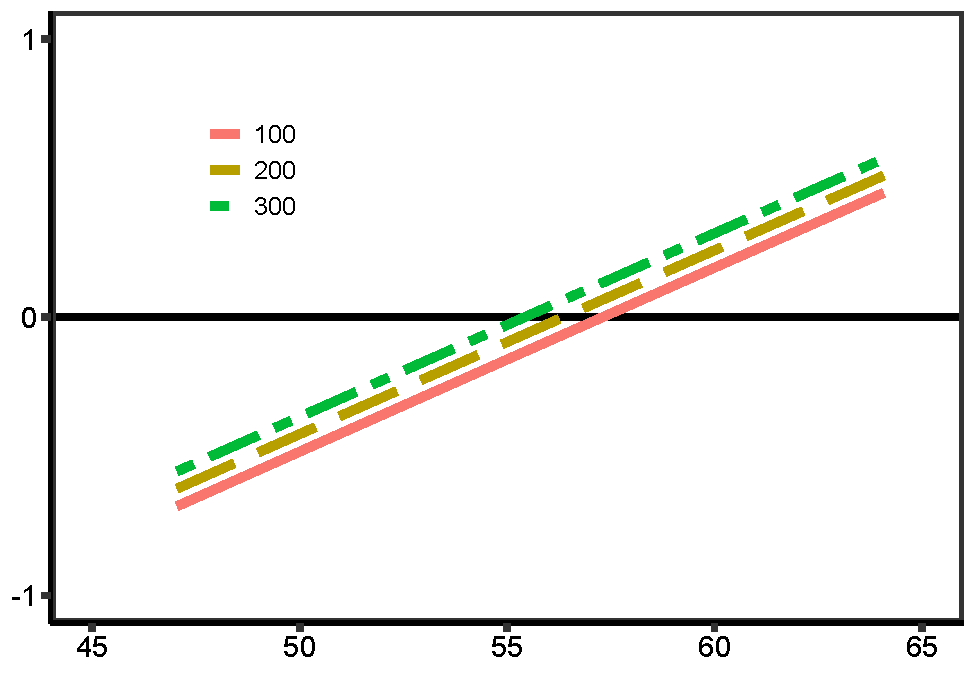
\includegraphics{bookdown_files/figure-latex/high3tplot-1.pdf}
\caption{\label{fig:high3tplot}不同导度下的 A VS Ci}
\end{figure}

\begin{Shaded}
\begin{Highlighting}[]
\NormalTok{data2 <-}\StringTok{ }\KeywordTok{read.csv}\NormalTok{(}\StringTok{"./data/DiffusionLimits.csv"}\NormalTok{)}
\NormalTok{data2}\OperatorTok{$}\NormalTok{Conductance <-}
\StringTok{  }\KeywordTok{revalue}\NormalTok{(}
\NormalTok{    data2}\OperatorTok{$}\NormalTok{Scenario,}
    \KeywordTok{c}\NormalTok{(}
      \StringTok{"Boundary Layer Conductance"}\NormalTok{ =}\StringTok{ "Boundary Layer"}\NormalTok{,}
      \StringTok{"Mesophyll Conductance"}\NormalTok{ =}\StringTok{ "Mesophyll"}\NormalTok{,}
      \StringTok{"Stomatal Conductance"}\NormalTok{ =}\StringTok{ "Stomatal"}
\NormalTok{    )}
\NormalTok{  )}
\NormalTok{cols <-}\StringTok{ }\KeywordTok{gg_color_hue}\NormalTok{(}\DecValTok{3}\NormalTok{)}

\NormalTok{Panel_1E <-}
\StringTok{  }\KeywordTok{ggplot}\NormalTok{(data2, }\KeywordTok{aes}\NormalTok{(}\DataTypeTok{x =}\NormalTok{ TotalRes, }\DataTypeTok{y =}\NormalTok{ Rates, }\DataTypeTok{colour =}\NormalTok{ Conductance)) }\OperatorTok{+}
\StringTok{  }\KeywordTok{geom_point}\NormalTok{(}\DataTypeTok{size =} \DecValTok{4}\NormalTok{) }\OperatorTok{+}
\StringTok{  }\KeywordTok{ggtitle}\NormalTok{(}\KeywordTok{expression}\NormalTok{(}\KeywordTok{paste}\NormalTok{(}\KeywordTok{bold}\NormalTok{(}\StringTok{"(e)"}\NormalTok{), }\StringTok{" Modelled Resistance Effect"}\NormalTok{))) }\OperatorTok{+}
\StringTok{  }\KeywordTok{labs}\NormalTok{(}\DataTypeTok{x =} \KeywordTok{expression}\NormalTok{(}\KeywordTok{paste}\NormalTok{(r[total] }\OperatorTok{*}\StringTok{ " (s"} \OperatorTok{~}\StringTok{ }\NormalTok{m }\OperatorTok{^}\StringTok{ }\NormalTok{\{}
    \DecValTok{2}
\NormalTok{  \} }\OperatorTok{~}\StringTok{ }\NormalTok{mol }\OperatorTok{^}\StringTok{ }\NormalTok{\{}
    \DecValTok{-1}
\NormalTok{  \} }\OperatorTok{*}\StringTok{ ")"}\NormalTok{)), }
  \DataTypeTok{y =} \KeywordTok{expression}\NormalTok{(}\KeywordTok{paste}\NormalTok{(C[c] }\OperatorTok{*}\StringTok{ " Ramp Rate ("} \OperatorTok{*}\StringTok{ }\NormalTok{mu }\OperatorTok{*}\StringTok{ }\NormalTok{mol }\OperatorTok{~}\StringTok{ }\NormalTok{mol }\OperatorTok{^}
\StringTok{                                    }\NormalTok{\{}
                                      \DecValTok{-1}
\NormalTok{                                    \} }\OperatorTok{~}\StringTok{ }\NormalTok{min }\OperatorTok{^}\StringTok{ }\NormalTok{\{}
                                      \DecValTok{-1}
\NormalTok{                                    \} }\OperatorTok{*}\StringTok{ ")"}\NormalTok{))) }\OperatorTok{+}
\StringTok{  }\KeywordTok{scale_x_continuous}\NormalTok{(}\DataTypeTok{limits =} \KeywordTok{c}\NormalTok{(}\DecValTok{0}\NormalTok{, }\DecValTok{50}\NormalTok{)) }\OperatorTok{+}
\StringTok{  }\KeywordTok{scale_y_continuous}\NormalTok{(}\DataTypeTok{limits =} \KeywordTok{c}\NormalTok{(}\DecValTok{0}\NormalTok{, }\DecValTok{80}\NormalTok{)) }\OperatorTok{+}
\StringTok{  }\KeywordTok{scale_color_manual}\NormalTok{(}
    \DataTypeTok{values =}\NormalTok{ cols,}
    \DataTypeTok{name =} \StringTok{"Manipulated Resistance"}\NormalTok{,}
    \DataTypeTok{labels =} \KeywordTok{c}\NormalTok{(}\StringTok{"Boundary Layer"}\NormalTok{, }\StringTok{"Mesophyll"}\NormalTok{, }\StringTok{"Stomatal"}\NormalTok{)}
\NormalTok{  ) }\OperatorTok{+}
\StringTok{  }\KeywordTok{theme_bw}\NormalTok{() }\OperatorTok{+}
\StringTok{  }\KeywordTok{theme}\NormalTok{(}
    \DataTypeTok{axis.title.x =} \KeywordTok{element_text}\NormalTok{(}\DataTypeTok{size =} \DecValTok{20}\NormalTok{),}
    \DataTypeTok{axis.title.y =} \KeywordTok{element_text}\NormalTok{(}\DataTypeTok{size =} \DecValTok{20}\NormalTok{),}
    \DataTypeTok{axis.line =} \KeywordTok{element_line}\NormalTok{(}\DataTypeTok{size =} \DecValTok{1}\NormalTok{),}
    \DataTypeTok{axis.ticks =} \KeywordTok{element_line}\NormalTok{(}\DataTypeTok{size =} \FloatTok{1.5}\NormalTok{),}
    \DataTypeTok{axis.ticks.length =} \KeywordTok{unit}\NormalTok{(}\FloatTok{1.5}\NormalTok{, }\StringTok{"mm"}\NormalTok{),}
    \DataTypeTok{rect =} \KeywordTok{element_rect}\NormalTok{(}\DataTypeTok{size =} \DecValTok{2}\NormalTok{),}
    \DataTypeTok{axis.text.x =} \KeywordTok{element_text}\NormalTok{(}\DataTypeTok{size =} \DecValTok{14}\NormalTok{, }\DataTypeTok{color =} \StringTok{'black'}\NormalTok{),}
    \DataTypeTok{axis.text.y =}
      \KeywordTok{element_text}\NormalTok{(}
        \DataTypeTok{size =} \DecValTok{14}\NormalTok{,}
        \DataTypeTok{color =} \StringTok{'black'}\NormalTok{,}
        \DataTypeTok{hjust =}\NormalTok{ (}\DecValTok{1}\NormalTok{)}
\NormalTok{      ),}
    \DataTypeTok{legend.position =} \KeywordTok{c}\NormalTok{(}\FloatTok{0.70}\NormalTok{, }\FloatTok{0.84}\NormalTok{),}
    \DataTypeTok{axis.title =} \KeywordTok{element_text}\NormalTok{(}\DataTypeTok{size =} \DecValTok{18}\NormalTok{),}
    \DataTypeTok{axis.text =} \KeywordTok{element_text}\NormalTok{(}\DataTypeTok{size =} \DecValTok{12}\NormalTok{, }\DataTypeTok{color =} \StringTok{"black"}\NormalTok{),}
    \DataTypeTok{panel.grid.major =} \KeywordTok{element_blank}\NormalTok{(),}
    \DataTypeTok{panel.grid.minor =} \KeywordTok{element_blank}\NormalTok{(),}
    \DataTypeTok{legend.text =} \KeywordTok{element_text}\NormalTok{(}\DataTypeTok{size =} \DecValTok{14}\NormalTok{),}
    \DataTypeTok{legend.title =} \KeywordTok{element_text}\NormalTok{(}\DataTypeTok{size =} \DecValTok{14}\NormalTok{)}
\NormalTok{  )}
\NormalTok{Panel_1E}
\end{Highlighting}
\end{Shaded}

\begin{figure}
\centering
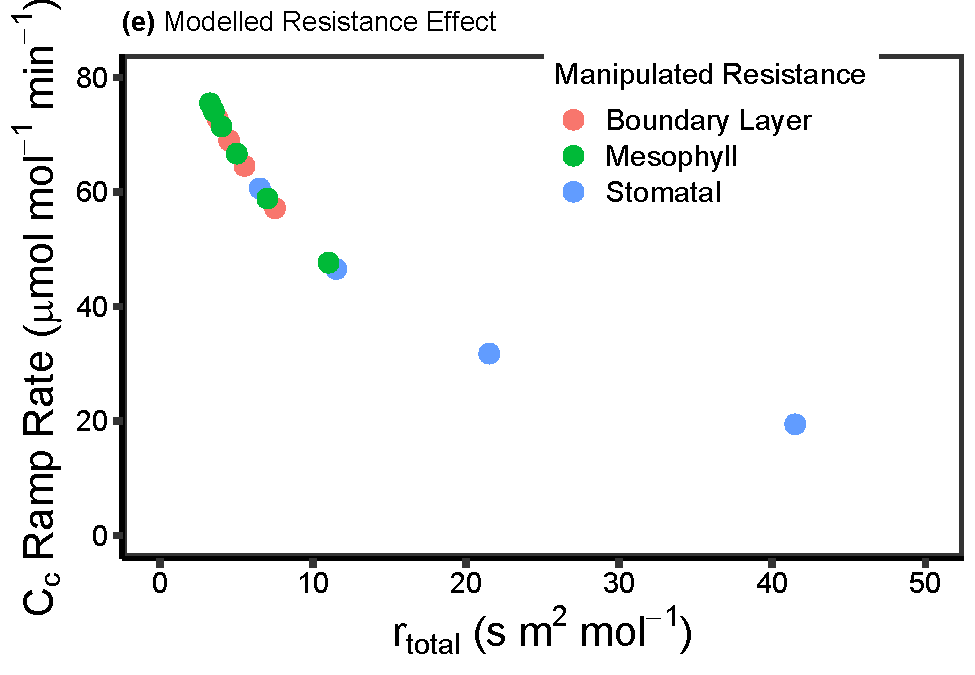
\includegraphics{bookdown_files/figure-latex/toresratetplot-1.pdf}
\caption{\label{fig:toresratetplot}不同总导度下的各个导度的变化}
\end{figure}

\begin{Shaded}
\begin{Highlighting}[]
\NormalTok{data <-}\StringTok{ }\KeywordTok{read.csv}\NormalTok{(}\StringTok{"./data/RASdata.csv"}\NormalTok{)}
\NormalTok{data}\OperatorTok{$}\NormalTok{Ccfull <-}\StringTok{ }\KeywordTok{as.numeric}\NormalTok{(data}\OperatorTok{$}\NormalTok{Ccfull)}
\NormalTok{data}\OperatorTok{$}\NormalTok{Deactivation <-}\StringTok{ }\KeywordTok{as.factor}\NormalTok{(data}\OperatorTok{$}\NormalTok{Deactivation)}
\KeywordTok{print}\NormalTok{(}\KeywordTok{levels}\NormalTok{(data}\OperatorTok{$}\NormalTok{Deactivation))}
\end{Highlighting}
\end{Shaded}

\begin{verbatim}
## [1] "High"   "Low"    "Medium" "None"
\end{verbatim}

\begin{Shaded}
\begin{Highlighting}[]
\NormalTok{data}\OperatorTok{$}\NormalTok{Deactivation <-}
\StringTok{  }\KeywordTok{factor}\NormalTok{(data}\OperatorTok{$}\NormalTok{Deactivation, }\KeywordTok{levels}\NormalTok{(data}\OperatorTok{$}\NormalTok{Deactivation)[}\KeywordTok{c}\NormalTok{(}\DecValTok{4}\NormalTok{, }\DecValTok{2}\NormalTok{, }\DecValTok{3}\NormalTok{, }\DecValTok{1}\NormalTok{)])}
\NormalTok{FigS1 <-}
\StringTok{  }\KeywordTok{ggplot}\NormalTok{(data,}
         \KeywordTok{aes}\NormalTok{(}
           \DataTypeTok{x =}\NormalTok{ Cifull,}
           \DataTypeTok{y =}\NormalTok{ Anet,}
           \DataTypeTok{colour =}\NormalTok{ Deactivation,}
           \DataTypeTok{linetype =}\NormalTok{ Deactivation}
\NormalTok{         )) }\OperatorTok{+}
\StringTok{  }\KeywordTok{geom_smooth}\NormalTok{(}\DataTypeTok{method =} \StringTok{"loess"}\NormalTok{, }\DataTypeTok{se =} \OtherTok{FALSE}\NormalTok{, }\DataTypeTok{size =} \DecValTok{2}\NormalTok{) }\OperatorTok{+}
\StringTok{  }\KeywordTok{scale_linetype_manual}\NormalTok{(}
    \DataTypeTok{name =} \StringTok{"Deactivation"}\NormalTok{,}
    \DataTypeTok{labels =} \KeywordTok{c}\NormalTok{(}\StringTok{"None"}\NormalTok{, }\StringTok{"Low"}\NormalTok{, }\StringTok{"Medium"}\NormalTok{, }\StringTok{"High"}\NormalTok{),}
    \DataTypeTok{values =} \KeywordTok{c}\NormalTok{(}\StringTok{"solid"}\NormalTok{, }\StringTok{"longdash"}\NormalTok{, }\StringTok{"dashed"}\NormalTok{, }\StringTok{"dotted"}\NormalTok{)}
\NormalTok{  ) }\OperatorTok{+}
\StringTok{  }\KeywordTok{labs}\NormalTok{(}\DataTypeTok{x =} \KeywordTok{expression}\NormalTok{(C[i] }\OperatorTok{~}\StringTok{ "("} \OperatorTok{*}\StringTok{ }\NormalTok{mu }\OperatorTok{*}\StringTok{ }\NormalTok{mol }\OperatorTok{~}\StringTok{ }\NormalTok{mol }\OperatorTok{^}\StringTok{ }\NormalTok{\{}
    \DecValTok{-1}
\NormalTok{  \} }\OperatorTok{*}\StringTok{ ")"}\NormalTok{),}
  \DataTypeTok{y =} \KeywordTok{expression}\NormalTok{(A[net] }\OperatorTok{~}\StringTok{ "("} \OperatorTok{*}\StringTok{ }\NormalTok{mu }\OperatorTok{*}\StringTok{ }\NormalTok{mol }\OperatorTok{~}\StringTok{ }\NormalTok{m }\OperatorTok{^}\StringTok{ }\NormalTok{\{}
    \DecValTok{-2}
\NormalTok{  \} }\OperatorTok{~}\StringTok{ }\NormalTok{s }\OperatorTok{^}\StringTok{ }\NormalTok{\{}
    \DecValTok{-1}
\NormalTok{  \} }\OperatorTok{*}\StringTok{ ")"}\NormalTok{)) }\OperatorTok{+}
\StringTok{  }\KeywordTok{labs}\NormalTok{(}\DataTypeTok{colour =} \StringTok{'Deactivation'}\NormalTok{) }\OperatorTok{+}
\StringTok{  }\KeywordTok{scale_x_continuous}\NormalTok{(}\DataTypeTok{limits =} \KeywordTok{c}\NormalTok{(}\DecValTok{25}\NormalTok{, }\DecValTok{100}\NormalTok{),}
                     \DataTypeTok{breaks =} \KeywordTok{c}\NormalTok{(}\DecValTok{25}\NormalTok{, }\DecValTok{40}\NormalTok{, }\DecValTok{55}\NormalTok{, }\DecValTok{70}\NormalTok{, }\DecValTok{85}\NormalTok{, }\DecValTok{100}\NormalTok{)) }\OperatorTok{+}
\StringTok{  }\KeywordTok{scale_y_continuous}\NormalTok{(}\DataTypeTok{limits =} \KeywordTok{c}\NormalTok{(}\OperatorTok{-}\DecValTok{5}\NormalTok{, }\DecValTok{5}\NormalTok{)) }\OperatorTok{+}
\StringTok{  }\KeywordTok{geom_hline}\NormalTok{(}\DataTypeTok{yintercept =} \DecValTok{0}\NormalTok{, }\DataTypeTok{size =} \FloatTok{1.5}\NormalTok{) }\OperatorTok{+}
\StringTok{  }\KeywordTok{theme_bw}\NormalTok{() }\OperatorTok{+}
\StringTok{  }\KeywordTok{theme}\NormalTok{(}
    \DataTypeTok{axis.title.x =} \KeywordTok{element_text}\NormalTok{(}\DataTypeTok{size =} \DecValTok{20}\NormalTok{),}
    \DataTypeTok{axis.title.y =} \KeywordTok{element_text}\NormalTok{(}\DataTypeTok{size =} \DecValTok{20}\NormalTok{),}
    \DataTypeTok{axis.line =} \KeywordTok{element_line}\NormalTok{(}\DataTypeTok{size =} \DecValTok{1}\NormalTok{),}
    \DataTypeTok{axis.ticks =} \KeywordTok{element_line}\NormalTok{(}\DataTypeTok{size =} \FloatTok{1.5}\NormalTok{),}
    \DataTypeTok{axis.ticks.length =} \KeywordTok{unit}\NormalTok{(}\FloatTok{1.5}\NormalTok{, }\StringTok{"mm"}\NormalTok{),}
    \DataTypeTok{rect =} \KeywordTok{element_rect}\NormalTok{(}\DataTypeTok{size =} \DecValTok{2}\NormalTok{),}
    \DataTypeTok{axis.text.x =} \KeywordTok{element_text}\NormalTok{(}\DataTypeTok{size =} \DecValTok{14}\NormalTok{, }\DataTypeTok{color =} \StringTok{'black'}\NormalTok{),}
    \DataTypeTok{axis.text.y =}
      \KeywordTok{element_text}\NormalTok{(}
        \DataTypeTok{size =} \DecValTok{14}\NormalTok{,}
        \DataTypeTok{color =} \StringTok{'black'}\NormalTok{,}
        \DataTypeTok{hjust =}\NormalTok{ (}\DecValTok{1}\NormalTok{)}
\NormalTok{      ),}
    \DataTypeTok{legend.position =} \KeywordTok{c}\NormalTok{(}\FloatTok{0.8}\NormalTok{, }\FloatTok{0.2}\NormalTok{),}
    \DataTypeTok{legend.text =} \KeywordTok{element_text}\NormalTok{(}\DataTypeTok{size =} \DecValTok{16}\NormalTok{),}
    \DataTypeTok{legend.title =} \KeywordTok{element_text}\NormalTok{(}\DataTypeTok{size =} \DecValTok{16}\NormalTok{),}
    \DataTypeTok{panel.grid.major =} \KeywordTok{element_blank}\NormalTok{(),}
    \DataTypeTok{panel.grid.minor =} \KeywordTok{element_blank}\NormalTok{()}
\NormalTok{  )}
\NormalTok{FigS1}
\end{Highlighting}
\end{Shaded}

\begin{figure}
\centering
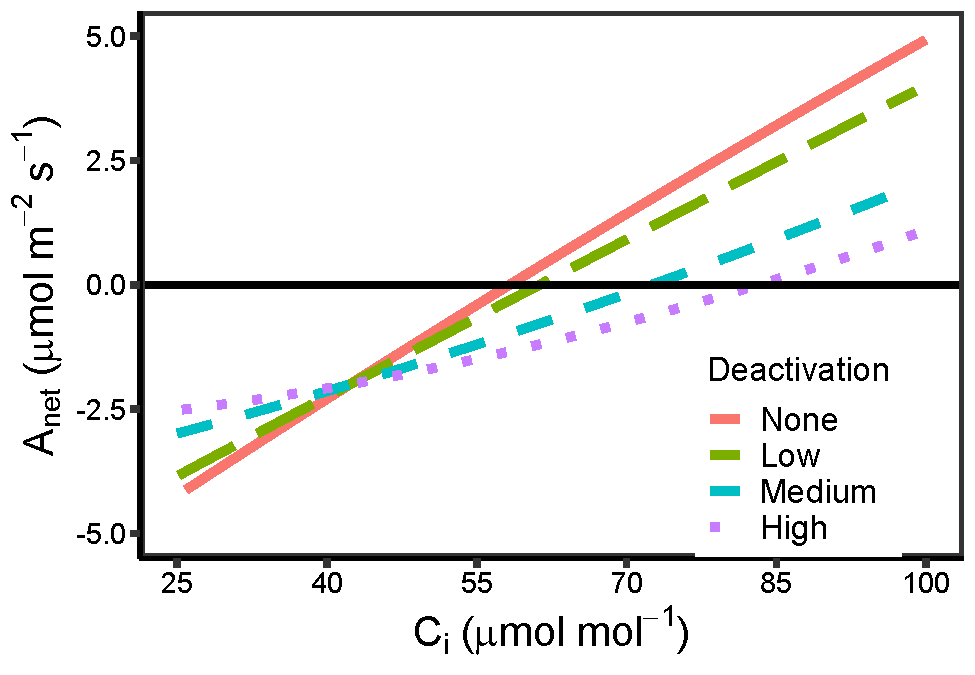
\includegraphics{bookdown_files/figure-latex/deasratetplot-1.pdf}
\caption{\label{fig:deasratetplot}Rubisco不同失活程度下的下 A VS Ci}
\end{figure}

\hypertarget{fluro68}{%
\section{LI-6800 荧光数据分析}\label{fluro68}}

LI-6800 能够直接提供基本的叶绿素荧光参数,其他参数均可通过这些基本的参数进行计算,计算也较简单,在此不赘述,需要注意的是快相荧光部分的数据,因为分析 ojip 数据的模型有很多,很多都需要复杂的计算,在此我们先将其中较为简单的 jip test 数据分析进行介绍。

\hypertarget{jiptest}{%
\subsection{jip test 的实现}\label{jiptest}}

LI-6800 增加了 ojip 曲线测量功能,本功能主要是针对测量数据的 jip test 的实现。

\hypertarget{jiptest_pack}{%
\subsection{\texorpdfstring{\texttt{jiptest} 软件包安装}{jiptest 软件包安装}}\label{jiptest_pack}}

目前 \texttt{jiptest} 暂时放在 github 我的软件仓库内,并没提交 CRAN,因此需要 \texttt{devtools} 的支持,然后才能从 github 安装 \texttt{jiptest}。

\begin{Shaded}
\begin{Highlighting}[]
\KeywordTok{install.packages}\NormalTok{(}\StringTok{"devtools"}\NormalTok{)}
\KeywordTok{library}\NormalTok{(devtools)}
\KeywordTok{install_github}\NormalTok{(}\StringTok{"zhujiedong/jiptest"}\NormalTok{)}
\end{Highlighting}
\end{Shaded}

\hypertarget{readfluor}{%
\subsection{\texorpdfstring{\texttt{read\_files} 及 \texttt{read\_dcfiles} 函数}{read\_files 及 read\_dcfiles 函数}}\label{readfluor}}

\texttt{read\_files} 用于批量读取所有调制光测量数据,方便用于其他的数据分析。\textbf{函数要求所有数据必须是 \texttt{xlsx} 格式,并且所有测量数据都保存在同一文件夹内。},如有其他文件或测量数据则会报错。
\texttt{read\_dcfiles} 用于批量读取所有连续光测量数据,其他与 \texttt{read\_dcfiles} 相同。

函数仅有一个参数,即保存数据文件夹的路径,使用如下:

\begin{Shaded}
\begin{Highlighting}[]
\KeywordTok{library}\NormalTok{(jiptest)}
\NormalTok{jipdata <-}\StringTok{ }\KeywordTok{read_files}\NormalTok{(}\StringTok{"./data/ojip"}\NormalTok{)}
\end{Highlighting}
\end{Shaded}

\begin{table}[t]

\caption{\label{tab:unnamed-chunk-51}jiptest 批量导入数据后的样式}
\centering
\begin{tabular}{rrl}
\toprule
SECS & FLUOR & SOURCE\\
\midrule
2.41e-05 & 887 & INDUCTION-484-20171225-13\_15\_58\\
2.81e-05 & 998 & INDUCTION-484-20171225-13\_15\_58\\
3.19e-05 & 1013 & INDUCTION-484-20171225-13\_15\_58\\
3.60e-05 & 1055 & INDUCTION-484-20171225-13\_15\_58\\
4.01e-05 & 1044 & INDUCTION-484-20171225-13\_15\_58\\
\addlinespace
4.41e-05 & 1205 & INDUCTION-484-20171225-13\_15\_58\\
\bottomrule
\end{tabular}
\end{table}

\begin{Shaded}
\begin{Highlighting}[]
\NormalTok{dcjipdata <-}\StringTok{ }\KeywordTok{read_dcfiles}\NormalTok{(}\StringTok{"./data/ojip"}\NormalTok{)}
\end{Highlighting}
\end{Shaded}

\begin{table}[t]

\caption{\label{tab:unnamed-chunk-52}jiptest DC 数据批量导入数据后的样式}
\centering
\begin{tabular}{rrl}
\toprule
SECS & FLUOR & SOURCE\\
\midrule
2.41e-05 & 154000 & INDUCTION-484-20171225-13\_15\_58\\
2.81e-05 & 157566 & INDUCTION-484-20171225-13\_15\_58\\
3.19e-05 & 161261 & INDUCTION-484-20171225-13\_15\_58\\
3.60e-05 & 165114 & INDUCTION-484-20171225-13\_15\_58\\
4.01e-05 & 169069 & INDUCTION-484-20171225-13\_15\_58\\
\addlinespace
4.41e-05 & 173231 & INDUCTION-484-20171225-13\_15\_58\\
\bottomrule
\end{tabular}
\end{table}

\hypertarget{testfluor}{%
\subsection{\texorpdfstring{\texttt{jip\_test} 及 \texttt{jip\_dctest} 函数}{jip\_test 及 jip\_dctest 函数}}\label{testfluor}}

\texttt{jiptest} 是 jiptest 的核心函数,用于所有数据的 jip test 分析,函数仅包一个参数,测量数据的保存文件夹路径。
\texttt{jip\_dctest} 与 \texttt{jip\_test} 相似,用于连续光测量数据的分析。

\begin{Shaded}
\begin{Highlighting}[]
\NormalTok{jip_results <-}\StringTok{ }\KeywordTok{jip_test}\NormalTok{(}\StringTok{"./data/ojip"}\NormalTok{)}
\end{Highlighting}
\end{Shaded}

\begin{verbatim}
## for the current version, we suggest you use the default settings of
## 
##   the duration (1000 ms or more) in the induction settings of LI-6800
\end{verbatim}

\begin{verbatim}
## New names:
## * `` -> ...1
## * `` -> ...2
## New names:
## * `` -> ...1
## * `` -> ...2
## New names:
## * `` -> ...1
## * `` -> ...2
## New names:
## * `` -> ...1
## * `` -> ...2
\end{verbatim}

\begin{longtable}{lrrrr}
\caption{\label{tab:jipres}jiptest 输出的计算参数}\\
\toprule
parameters & data\_file1 & data\_file2 & data\_file3 & data\_file4\\
\midrule
Fo & 887.000 & 849.000 & 981.000 & 914.000\\
Fm & 4649.520 & 3714.270 & 4225.240 & 3754.270\\
F300 & 2181.400 & 1798.600 & 2067.800 & 2537.200\\
FJ & 2594.300 & 2104.600 & 2456.800 & 2569.000\\
FI & 4443.110 & 3547.110 & 4009.220 & 3556.530\\
\addlinespace
Tfmax & 256.016 & 316.016 & 272.016 & 200.016\\
\bottomrule
\end{longtable}

\begin{Shaded}
\begin{Highlighting}[]
\NormalTok{dcjip_results <-}\StringTok{ }\KeywordTok{jip_dctest}\NormalTok{(}\StringTok{"./data/ojip"}\NormalTok{)}
\end{Highlighting}
\end{Shaded}

\begin{longtable}{lrrrr}
\caption{\label{tab:dcjipres}jiptest DC 数据输出的计算参数}\\
\toprule
parameters & data\_file1 & data\_file2 & data\_file3 & data\_file4\\
\midrule
Fo & 154000.000 & 133191.000 & 156664.000 & 153589.000\\
Fm & 713839.000 & 560610.000 & 647660.000 & 584839.000\\
F300 & 338091.000 & 275476.800 & 322859.200 & 388110.400\\
FJ & 400744.000 & 320245.000 & 376885.000 & 406671.000\\
FI & 681505.000 & 534314.000 & 614590.000 & 552253.000\\
\addlinespace
Tfmax & 276.016 & 300.016 & 288.016 & 212.016\\
\bottomrule
\end{longtable}

计算参数见表 \ref{tab:jipres} 及 \ref{tab:dcjipres},考虑到排版,仅显示部分内容。若需要将数据导出,可以使用相关命令,如:

\begin{Shaded}
\begin{Highlighting}[]
\CommentTok{# export the results of jiptest to a csv file}
\KeywordTok{write.csv}\NormalTok{(jip_results, }\StringTok{"d:/data/jip_resluts.csv"}\NormalTok{)}
\KeywordTok{write.csv}\NormalTok{(dcjip_results, }\StringTok{"d:/data/dcjip_resluts.csv"}\NormalTok{)}
\end{Highlighting}
\end{Shaded}

\hypertarget{plotfluor}{%
\subsection{\texorpdfstring{\texttt{jip\_plot} 及 \texttt{jip\_dcplot} 函数}{jip\_plot 及 jip\_dcplot 函数}}\label{plotfluor}}

\texttt{jip\_plot} 和 \texttt{jip\_dcplot} 基于 \texttt{ggplot2},用于快速预览所有测量结果的 ojip 曲线。函数仅有一个参数,即保存数据文件夹的路径,使用如下:

\begin{Shaded}
\begin{Highlighting}[]
\KeywordTok{jip_plot}\NormalTok{(}\StringTok{"./data/ojip"}\NormalTok{)}
\end{Highlighting}
\end{Shaded}

\begin{figure}
\centering
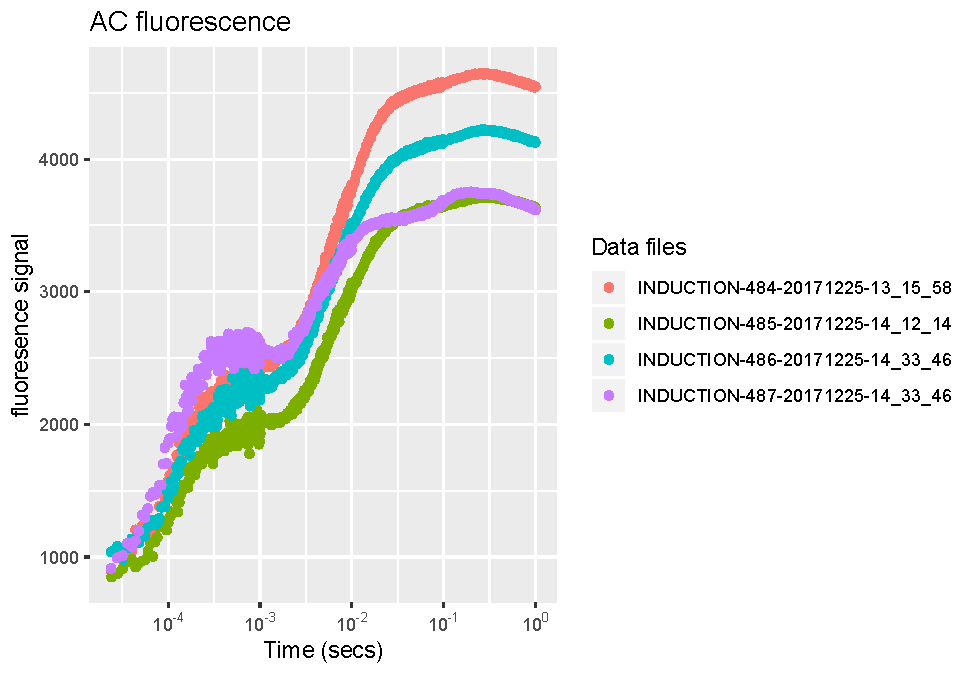
\includegraphics{bookdown_files/figure-latex/acplot-1.pdf}
\caption{\label{fig:acplot}调制式测量的 ojip 曲线的快速预览}
\end{figure}

\begin{Shaded}
\begin{Highlighting}[]
\KeywordTok{jip_dcplot}\NormalTok{(}\StringTok{"./data/ojip"}\NormalTok{)}
\end{Highlighting}
\end{Shaded}

\begin{figure}
\centering
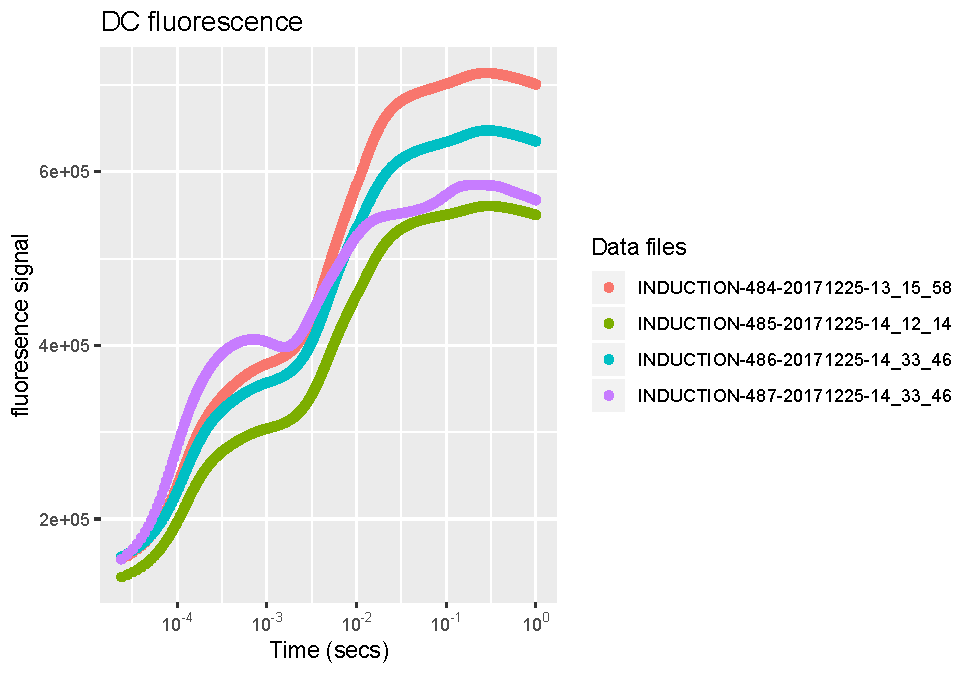
\includegraphics{bookdown_files/figure-latex/dcplot-1.pdf}
\caption{\label{fig:dcplot}连续式测量的 ojip 曲线的快速预览}
\end{figure}

ojip 调制式测量光 ojip 曲线的快速预览如图 \ref{fig:acplot}

ojip 连续式测量光 ojip 曲线的快速预览如图 \ref{fig:dcplot}

\textbf{建议在开始分析数据前,使用如上方式作图查看数据质量,若使用调制光数据测量的荧光信号太弱,数据点太散,则可以使用连续光测量信号进行分析,对于归一化的荧光参数,二者几乎无差别,当然避免陷入被动的最好方式还是最开始测量时注意检查数据质量}

\cleardoublepage

\hypertarget{pca-anylysis}{%
\chapter{大话 PCA}\label{pca-anylysis}}

PCA 作为一个基础的方法,应用领域覆盖很广,涵盖的统计学相关的内容有均值、标准差、协方差, 线性代数中的特征向量及特征值。当然在与光合仪相关的应用方面多数是测量的光合速率、气孔导度等配合植物的其他性状来进行研究,其适用范围,用现在流行的统计学习术语来讲,应属于非监督性学习,即我们并非预测某变量同其预测值的关系,如同我们获得了一系列包含植物光合性状在内的性状,但我们并非将其预测某些结果,如同响应曲线那般,而是用这些形状来分类或者看齐对某目的的重要程度。本章的标题之所以叫大话,是因为这是我结合我自己的理解写的内容,如有错误请谅解,请指出。

另,推荐两个我认为很好的解释 PCA 的链接:

\href{https://blog.bioturing.com/2018/06/14/principal-component-analysis-explained-simply/}{BioTuring's Blog}

\href{http://setosa.io/ev/principal-component-analysis/}{Principal Component Analysis}

\hypertarget{geom-pca}{%
\section{几何解释}\label{geom-pca}}

PCA 通常能够反映我们复杂数据集的一些分布特征,例如典型的 \texttt{iris} 数据集,我们看到了三个鸢尾种的四个性状:花萼的长宽、花瓣的长宽,如果给我们这么一个数据,我们肉眼很难看出他们的特征来,如果作图也很难表达,因为这是一个四维的数据,假设我们只对前两组也就是花萼的长宽作图,先看一下二维的数据情况:

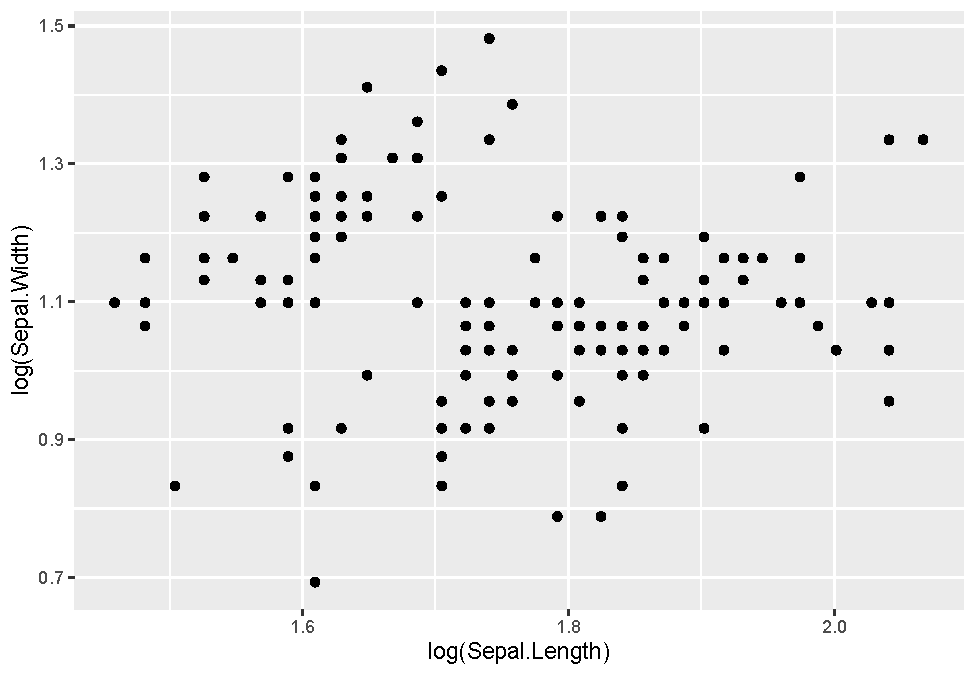
\includegraphics{bookdown_files/figure-latex/2dim-1.pdf}

看上去一言难尽,此时的缺点非常明显,图中的每个点均代表了某个植株的两个性状,这个性状类似于我们说的电子云,杂乱而无规律。这还只是二维数据,如果我们将所有四个轴的数据都显示也就是四维的数据,那么对于我等肉眼凡胎来讲,还是不看为妙。

我在看到上面留的两个网址之前,对主成份分析的疑惑一直没断过,什么是主成份,一直说是主轴旋转,到底是怎么旋转的,我们看一下主成份的 PC1 是怎么来做的:

\begin{figure}
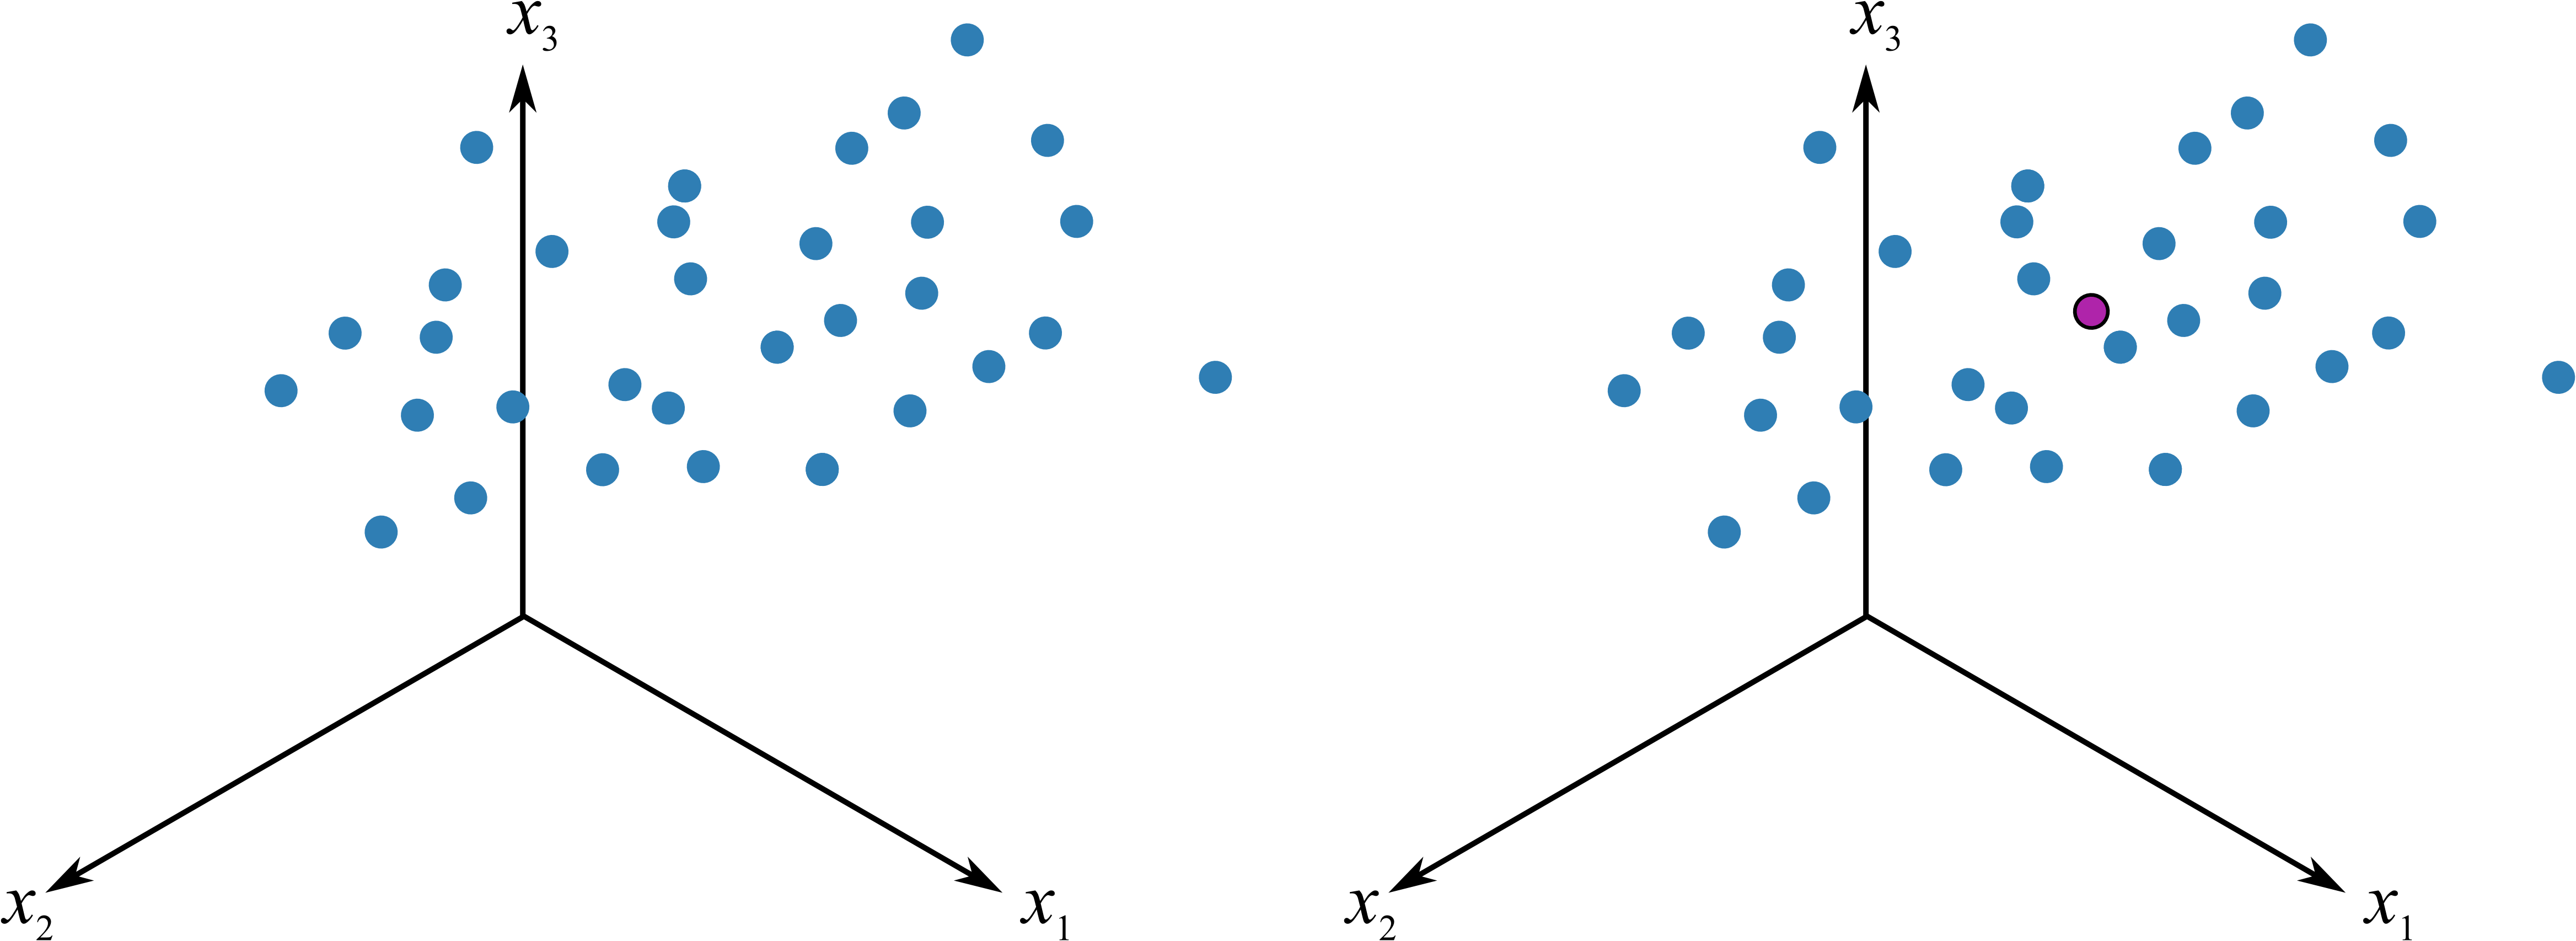
\includegraphics[width=1\linewidth]{images/pc1} \caption{数据的中心化}\label{fig:pccenter}
\end{figure}

如图 \ref{fig:pccenter},假设有三维的数据,可以理解为 iris 数据中前三列的观测值,每个点分别代表了一个植株的前三个性状,PCA 第一步便是中心化,将坐标轴由左边转移到右边的中心点位置作为原点,这就是所谓的平均值中心化的过程,这样就消除了测量时的偏差 \footnote{\url{https://www.mathsisfun.com/definitions/bias.html}},同时一般还要对数据进行缩放,以消除不同单位的影响 \footnote{\url{https://en.wikipedia.org/wiki/Scaling_(geometry)}},
例如有光合速率,有叶片面积的数据,这样能够消除不同单位的影响,通常的缩放例如对数化。

\begin{figure}
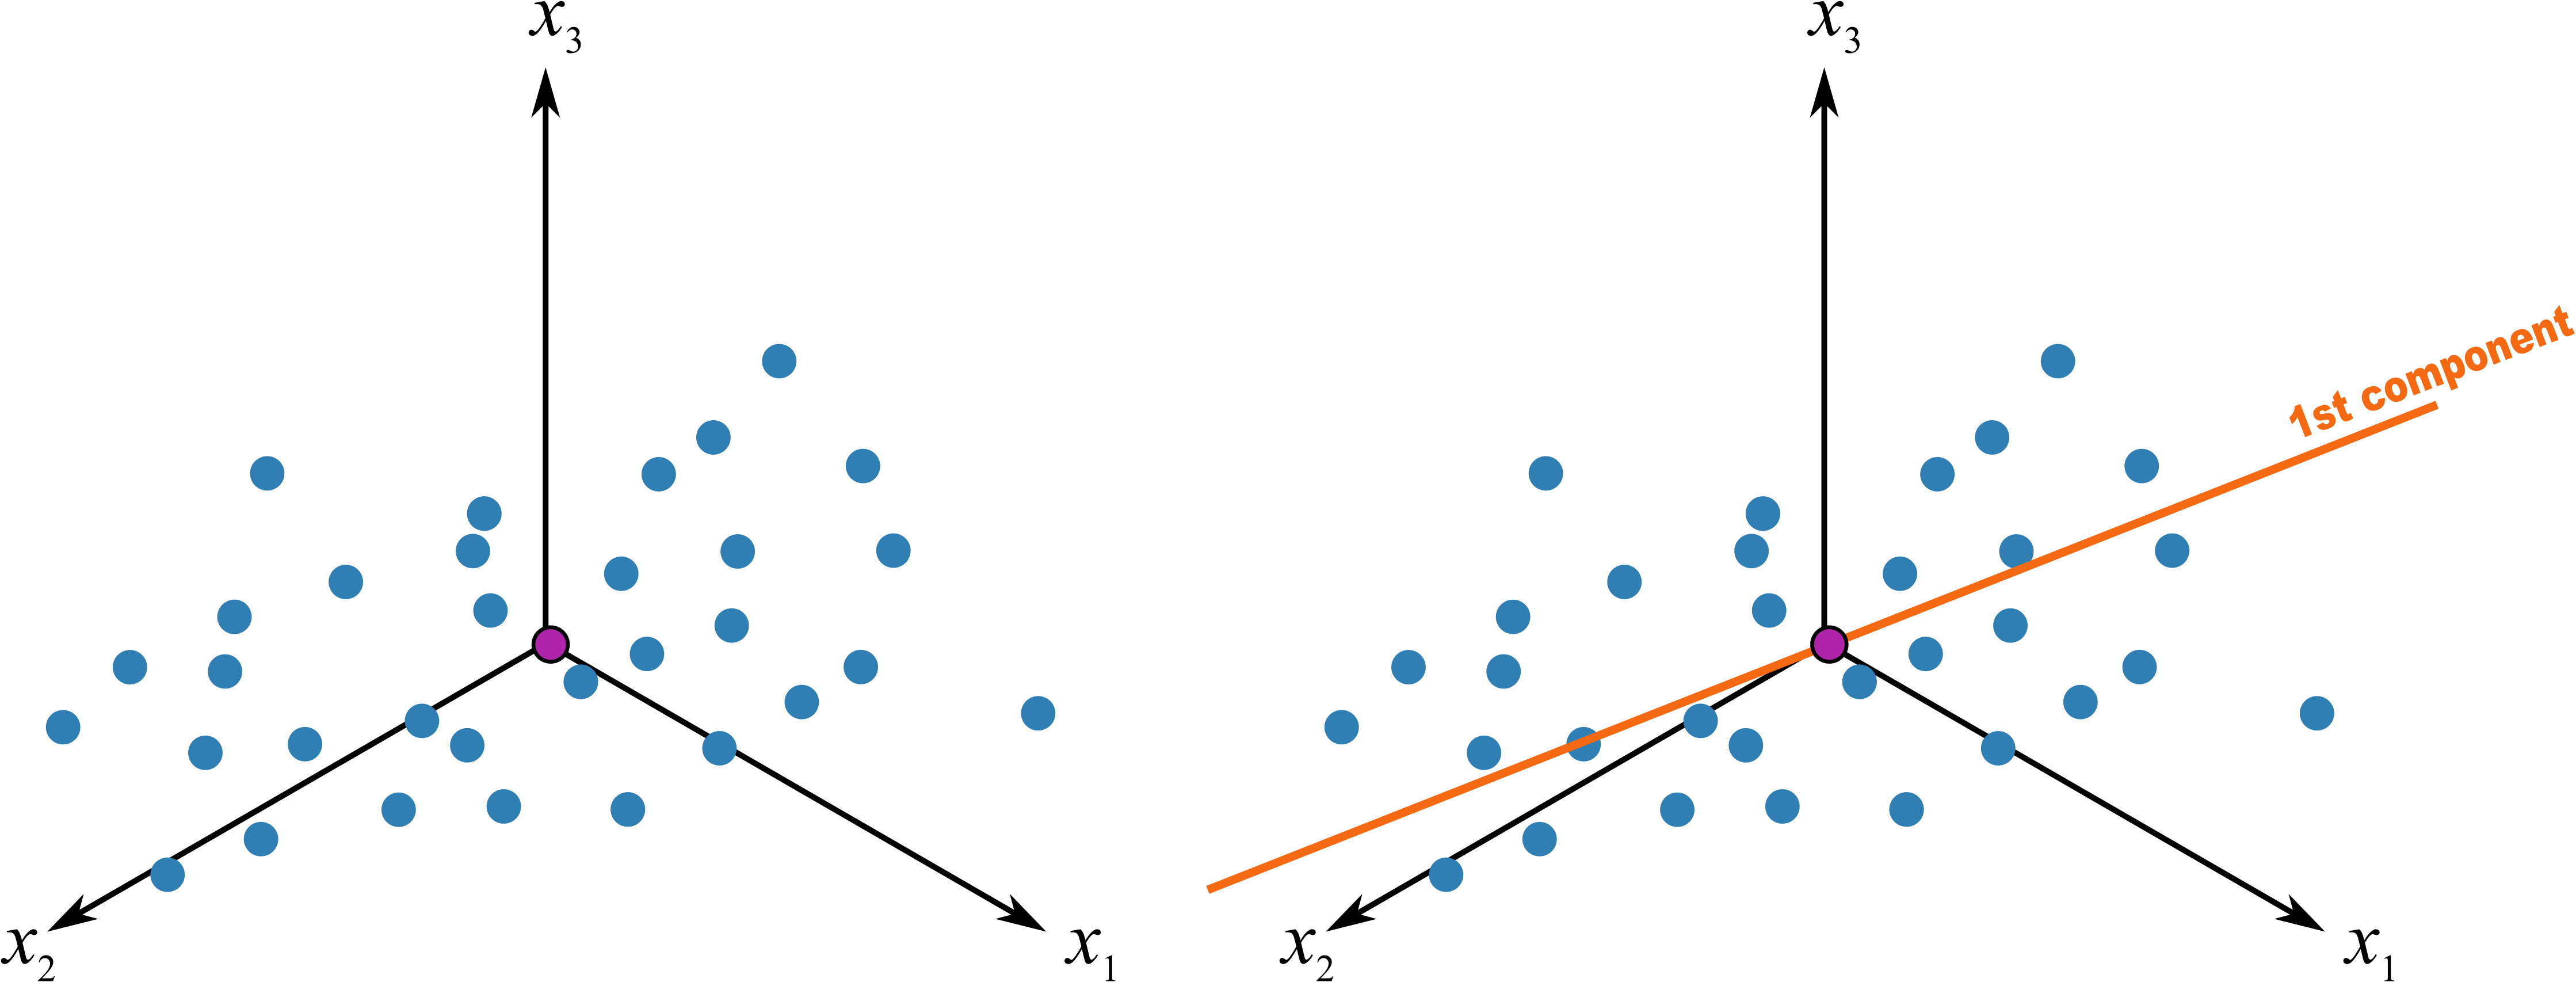
\includegraphics[width=1\linewidth]{images/pc2} \caption{PC1 的诞生}\label{fig:pc2}
\end{figure}

移动坐标系后,因为进行了缩放,所有的数据具有相同的比例。我们这时做一条最佳的拟合线(图 \ref{fig:pc2}),此时发生了两件重要的事情:

\begin{itemize}
\tightlist
\item
  所有的点投影到这条拟合线上,投影后的点之间的距离是最大的,该方向代表了所有变异最大,也就是最大化的区分所有的数据点,因为我们的目的就是要区分数据点之间的差异。如果在读的各位有跟我一样空间想象力有限的,可以根据图 \ref{fig:maxvar} 的极端情况来理解,蓝色线为最佳拟合线,红色的数据点投影到其上的距离之和当然大于投影到蓝色的拟合线上。
\end{itemize}

\begin{figure}
\centering
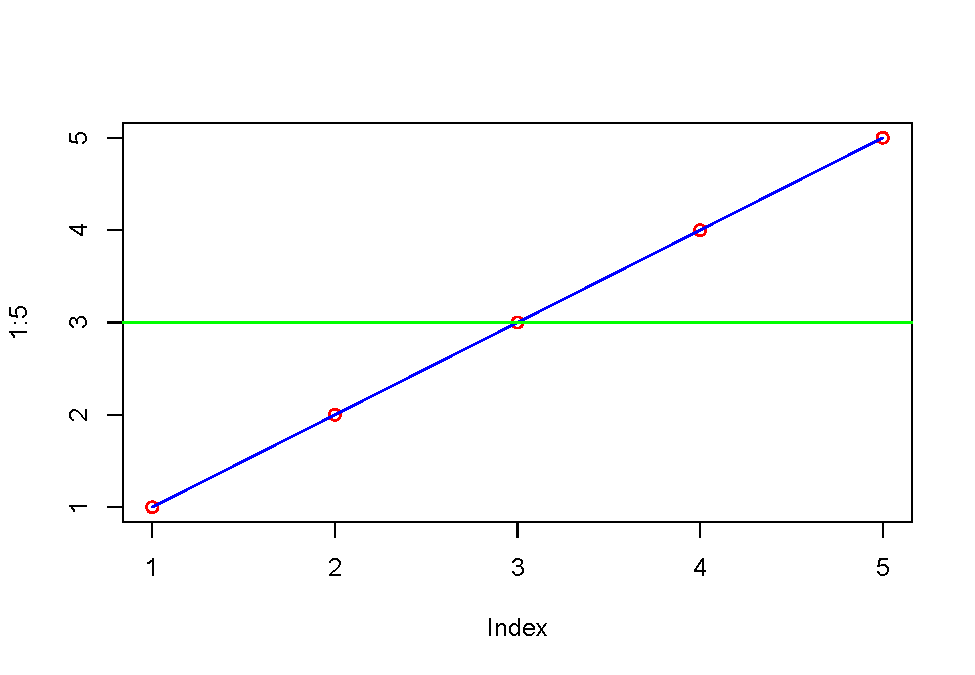
\includegraphics{bookdown_files/figure-latex/maxvar-1.pdf}
\caption{\label{fig:maxvar}变异最大的极端情况}
\end{figure}

\begin{itemize}
\tightlist
\item
  所有点和他们相对应的点之间的距离是最小的(也就是残差最小,最佳拟合当然是残差最小),这保证了这些投影的点和原来的数据点尽可能接近,也就是变化后损失的信息最少。
\end{itemize}

以上变化的最终结果为将变异放到最大而误差降低到最小,我们研究的最终目的无非就是这样。这个最佳拟合的线我们将其称之为 PC1,主成份1。

\begin{figure}
\includegraphics[width=1\linewidth]{images/pc3} \caption{PC2 的诞生}\label{fig:pc3}
\end{figure}

如果我们做一条通过中心点并与 PC1 垂直的线,并不断旋转这条线使其满足:所有投影于其上的点,他们的距离最大,也就是变异最大,这样就做出了第二个主成份,PC2,如图 \ref{fig:pc3}。\textbf{就这样不断的变换,一般情况下,我们可以使用 2\textasciitilde{}3 个主成份来解释绝大部分数据所展示的信息(所有数据都尽可能少的损失信息投影于其上)}。

以上为基本变换,如果我们使用 R 计算 PCA (这里推荐两个包 \texttt{factoextra} 和 \texttt{FactoMineR}),查看其结果:

\begin{Shaded}
\begin{Highlighting}[]
\KeywordTok{library}\NormalTok{(}\StringTok{"FactoMineR"}\NormalTok{)}
\KeywordTok{library}\NormalTok{(}\StringTok{"factoextra"}\NormalTok{)}
\end{Highlighting}
\end{Shaded}

\begin{verbatim}
## Welcome! Related Books: `Practical Guide To Cluster Analysis in R` at https://goo.gl/13EFCZ
\end{verbatim}

\begin{Shaded}
\begin{Highlighting}[]
\NormalTok{ir <-}\StringTok{ }\NormalTok{iris[, }\DecValTok{1}\OperatorTok{:}\DecValTok{4}\NormalTok{]}
\NormalTok{ir_pca <-}\StringTok{ }\KeywordTok{PCA}\NormalTok{(ir, }\DataTypeTok{graph =} \OtherTok{FALSE}\NormalTok{)}

\KeywordTok{fviz_eig}\NormalTok{(ir_pca, }\DataTypeTok{addlabels =} \OtherTok{TRUE}\NormalTok{)}
\end{Highlighting}
\end{Shaded}

\begin{figure}
\centering
\includegraphics{bookdown_files/figure-latex/scree-1.pdf}
\caption{\label{fig:scree}iris 碎石图}
\end{figure}

我们可以看到,前两个成分可以解释数据 95\% 以上的变异,所以我们可以只使用主成份 1 和主成份 2 对我们的结果进行解释。

既然我们使用两个主成份解释整个数据,那么我们怎么把四个性状都放在这个图上呢?这就需要载荷图来展示了,如图 \ref{fig:loadingpca}

\begin{Shaded}
\begin{Highlighting}[]
\KeywordTok{fviz_pca_var}\NormalTok{(ir_pca)}
\end{Highlighting}
\end{Shaded}

\begin{figure}
\centering
\includegraphics{bookdown_files/figure-latex/loadingpca-1.pdf}
\caption{\label{fig:loadingpca}iris 载荷图}
\end{figure}

怎么解释呢,因为原始的数据点相当于在坐标轴上,这几个性状分布的产生类似于原始的数据点在拉拽某个性状,影响强的偏向某一方向,换句话说,\textbf{这些性状决定主成份时有不同的权重,也就是对主成份影响的权重大小。同时他们是有方向的,如果两个性状方向接近,也就是夹角非常小,说明他们有较强的正相关性,例如图中的花瓣的长宽,如果他们互相垂直,那说明他们无相关性,例如图中花萼的长宽,如果夹角非常大,例如他们几乎在一条直线上,说明具有显著的负相关}。其本质还是所有的单位向量(本例有四个性状,各个性状中心化后形成的轴,也就是向量)在现在的这个二维平面的位置。

而如果我想通过这些性状来对鸢尾分类,怎么看呢?那就需要得分图来展示了,如图 \ref{fig:scorepca} ,得分图本质是各个品种的每个观测值在各个轴上的长度,也就是得分,所以其值都是每个物种性状的加权,每个点代表了每个物种的观测值。

\begin{Shaded}
\begin{Highlighting}[]
\KeywordTok{fviz_pca_ind}\NormalTok{(ir_pca, }\DataTypeTok{repel =} \OtherTok{TRUE}\NormalTok{, }\DataTypeTok{col.ind=}\NormalTok{ iris}\OperatorTok{$}\NormalTok{Species)}
\end{Highlighting}
\end{Shaded}

\begin{figure}
\centering
\includegraphics{bookdown_files/figure-latex/scorepca-1.pdf}
\caption{\label{fig:scorepca}iris 得分图}
\end{figure}

我们明显看出来,PC1 方向,三个种的鸢尾分成了两大部分,其中 Setosa 延 PC1 同其他两个明显有区别,另外两个在 PC1 上也有较明显的区别,但二者有一定的重合,延 PC2 方向上,三者差别不大。或者反过来讲也可以,品种的差别对 PC1 影响比较显著,这也和我们的碎石图相匹配。

\hypertarget{alge-pca}{%
\section{线性代数解释}\label{alge-pca}}

\hypertarget{egi-pca}{%
\subsection{特征向量与特征值}\label{egi-pca}}

特征向量和特征值的数学描述为:

\begin{equation}
A \vec{x} = \lambda \vec{x}
\label{eq:eign}
\end{equation}

其中 A 为 n \(\times\) n 的矩阵,\(\vec{x}\) 为 非零 n \(\times\) 1 列向量,\(\lambda\) 是标量,那么 \(\vec{x}\) 为 A 的特征向量,\(\lambda\) 为 A 的特征值。

如果仅从数学描述上看,是十分不适合我这样没基础的人来理解的,但我们可以这么理解:

A 为我们观测值(也即我们生态学上测量的数据)组成的 \(n \times n\) 矩阵,每行的数据代表了一个观测值,例如光合速率是其中的一行,我们有n 个, 那么 \(\vec{x}\) 和 \(\lambda\) 意味着什么呢?再看一眼上面的 \eqref{eq:eign},这是一个等式,而 \(\vec{x}\) 是 n \(\times\) 1 维度,原来的数据是 n \(\times\) n 维度,这就是主轴分析是降维分析的意义了,一个一维的特征向量和特征值与我们多维的观测值之间有一个相等的关系。当然,也有很多人在描述时喜欢用坐标轴旋转或这投影来形容的,如果你觉得这样好理解也没问题,不过我脑袋不擅长想象这种多维的空间。这样描述并不十分准确,只是我觉得便于理解,更正确描述应为我们下面所述的例子 (\citet{Smith2002}) ,但降维的原理即来自此处:

\begin{equation}
finaldata = rowfeaturevector \times rowdataajust
\label{eq:despca}
\end{equation}

finaldata 很好理解,我们用于 PCA 的最终数据,rowfeature vector 则是我们根据协相关矩阵求得的特征向量的转置,最大的特征向量再最上面, rowdataadjust 则为\textbf{原始数据减去标准值}。

因为我手头没有相关的数据,想来想去,我们在 R 里见到最多的与生态学相关的数据也就是 iris,一个关于不同 iris 品种的叶片性状相关的数据,非常生态,我们还是继续使用:

\begin{tabular}{r|r|r|r|l}
\hline
Sepal.Length & Sepal.Width & Petal.Length & Petal.Width & Species\\
\hline
5.1 & 3.5 & 1.4 & 0.2 & setosa\\
\hline
4.9 & 3.0 & 1.4 & 0.2 & setosa\\
\hline
4.7 & 3.2 & 1.3 & 0.2 & setosa\\
\hline
4.6 & 3.1 & 1.5 & 0.2 & setosa\\
\hline
5.0 & 3.6 & 1.4 & 0.2 & setosa\\
\hline
5.4 & 3.9 & 1.7 & 0.4 & setosa\\
\hline
\end{tabular}

数据并不复杂,但是想要得出一些规律性的东西确不那么容易,因为数据量太大了。R 语言里面很多函数可以直接实现 PCA,例如 \ref{geom-pca} 内容。这里按照最原始的方法实现一下,加深对原理的理解:

\hypertarget{man_pca}{%
\subsection{手动实现过程}\label{man_pca}}

\hypertarget{av_val}{%
\subsubsection{均值的计算}\label{av_val}}

\begin{Shaded}
\begin{Highlighting}[]
\NormalTok{iris_mean <-}\StringTok{ }\KeywordTok{apply}\NormalTok{(iris[, }\DecValTok{1}\OperatorTok{:}\DecValTok{4}\NormalTok{], }\DecValTok{2}\NormalTok{, }\ControlFlowTok{function}\NormalTok{(x) x }\OperatorTok{-}\StringTok{ }\KeywordTok{mean}\NormalTok{(x))}
\end{Highlighting}
\end{Shaded}

我只使用了前四列的性状数据,仅仅是方便结果的展示。

\hypertarget{cov_val}{%
\subsubsection{计算协方差矩阵}\label{cov_val}}

\begin{Shaded}
\begin{Highlighting}[]
\NormalTok{iris_cov <-}\StringTok{ }\KeywordTok{cov}\NormalTok{(iris_mean)}
\end{Highlighting}
\end{Shaded}

\hypertarget{eig_val}{%
\subsubsection{计算特征值和特征向量}\label{eig_val}}

\begin{Shaded}
\begin{Highlighting}[]
\NormalTok{iris_eigen <-}\StringTok{ }\KeywordTok{eigen}\NormalTok{(iris_cov)}
\end{Highlighting}
\end{Shaded}

这里就可以看到之前提到的,特征值和特征向量是根据协方差矩阵计算的。我们选取特征值最大的两个,他们的特征值之和已经占所有的特征值之和相当大的比例:

\begin{Shaded}
\begin{Highlighting}[]
\KeywordTok{sum}\NormalTok{(iris_eigen}\OperatorTok{$}\NormalTok{values[}\DecValTok{1}\OperatorTok{:}\DecValTok{2}\NormalTok{])}\OperatorTok{/}\KeywordTok{sum}\NormalTok{(iris_eigen}\OperatorTok{$}\NormalTok{values)}
\end{Highlighting}
\end{Shaded}

\begin{verbatim}
## [1] 0.9776852
\end{verbatim}

也就是说特征值对应的前两项是我们最终降维所需要的,即最终的两个主轴为 \(150 \times 2\) 维矩阵,即我们原来的 \(150 \times 4\) 的矩阵乘以我们选取的前两个特征值对应的 \(4 \times 2\) 组成的矩阵。

实际应用中我们不需要这么做了,因为太浪费时间了,我们直接用函数来得到结果即可。

\hypertarget{prcom}{%
\subsection{\texorpdfstring{\texttt{prcomp} 的实现}{prcomp 的实现}}\label{prcom}}

我们用 \texttt{prcomp} 来简化实现过程,注意,根据 \citet{kemp2003modern},我们把 iris 数据对数化一下,并提取所有物种名字:

\begin{Shaded}
\begin{Highlighting}[]
\KeywordTok{data}\NormalTok{(}\StringTok{"iris"}\NormalTok{)}
\NormalTok{iris_pca <-}\StringTok{ }\KeywordTok{log}\NormalTok{(iris[, }\DecValTok{1}\OperatorTok{:}\DecValTok{4}\NormalTok{])}
\NormalTok{iris_species <-}\StringTok{ }\NormalTok{iris}\OperatorTok{$}\NormalTok{Species}
\end{Highlighting}
\end{Shaded}

需要注意,我们处理时使用特征中心化。即每一维的数据都减去该维的均值。这里的``维''指的就是一个特征(或属性),变换之后每一维的均值都变成了0 (参考 \eqref{eq:despca} )。

\begin{Shaded}
\begin{Highlighting}[]
\NormalTok{value_pca <-}\StringTok{ }\KeywordTok{prcomp}\NormalTok{(iris_pca, }\DataTypeTok{center =} \OtherTok{TRUE}\NormalTok{, }\DataTypeTok{scale. =} \OtherTok{TRUE}\NormalTok{)}
\CommentTok{## 查看结果}
\KeywordTok{summary}\NormalTok{(value_pca)}
\end{Highlighting}
\end{Shaded}

\begin{verbatim}
## Importance of components:
##                           PC1    PC2     PC3     PC4
## Standard deviation     1.7125 0.9524 0.36470 0.16568
## Proportion of Variance 0.7331 0.2268 0.03325 0.00686
## Cumulative Proportion  0.7331 0.9599 0.99314 1.00000
\end{verbatim}

可以看到结果同我们最开始的计算相似,不同的是我们进行了对数化,而且根据 \citet{kemp2003modern}, 这个结果更合适。

\hypertarget{sessioninfo}{%
\chapter{环境与配置}\label{sessioninfo}}

本文的内容所完成的 sessioninfo 如下:

\begin{Shaded}
\begin{Highlighting}[]
\KeywordTok{sessionInfo}\NormalTok{()}
\end{Highlighting}
\end{Shaded}

\begin{verbatim}
## R version 3.6.0 (2019-04-26)
## Platform: x86_64-w64-mingw32/x64 (64-bit)
## Running under: Windows 10 x64 (build 17763)
## 
## Matrix products: default
## 
## locale:
## [1] LC_COLLATE=Chinese (Simplified)_China.936 
## [2] LC_CTYPE=Chinese (Simplified)_China.936   
## [3] LC_MONETARY=Chinese (Simplified)_China.936
## [4] LC_NUMERIC=C                              
## [5] LC_TIME=Chinese (Simplified)_China.936    
## 
## attached base packages:
## [1] stats     graphics  grDevices utils     datasets  methods   base     
## 
## other attached packages:
##  [1] factoextra_1.0.5   FactoMineR_1.41    jiptest_0.1.3     
##  [4] gridExtra_2.3      plyr_1.8.4         racir_1.0.0       
##  [7] nls2_0.2           proto_1.0.0        purrr_0.3.2       
## [10] ggplot2_3.1.1      minpack.lm_1.2-1   plantecophys_1.4-4
## [13] readphoto_0.0.1   
## 
## loaded via a namespace (and not attached):
##  [1] tidyselect_0.2.5     xfun_0.6             lattice_0.20-38     
##  [4] colorspace_1.4-1     htmltools_0.3.6      yaml_2.2.0          
##  [7] rlang_0.3.4          ggpubr_0.2           pillar_1.3.1        
## [10] glue_1.3.1           withr_2.1.2          RColorBrewer_1.1-2  
## [13] readxl_1.3.1         stringr_1.4.0        munsell_0.5.0       
## [16] gtable_0.3.0         cellranger_1.1.0     leaps_3.0           
## [19] evaluate_0.13        labeling_0.3         geepack_1.2-1       
## [22] knitr_1.22           highr_0.8            Rcpp_1.0.1          
## [25] flashClust_1.01-2    scales_1.0.0         scatterplot3d_0.3-41
## [28] png_0.1-7            digest_0.6.18        stringi_1.4.3       
## [31] ggrepel_0.8.0        bookdown_0.9         dplyr_0.8.0.1       
## [34] grid_3.6.0           tools_3.6.0          magrittr_1.5        
## [37] lazyeval_0.2.2       tibble_2.1.1         cluster_2.0.8       
## [40] MESS_0.5.5           crayon_1.3.4         geeM_0.10.1         
## [43] pkgconfig_2.0.2      MASS_7.3-51.4        Matrix_1.2-17       
## [46] assertthat_0.2.1     rmarkdown_1.12       rematch_1.0.1       
## [49] rstudioapi_0.10      R6_2.4.0             compiler_3.6.0
\end{verbatim}

\cleardoublepage

  \bibliography{photoR.bib}

\backmatter
\printindex

\end{document}
